\documentclass[a4paper, 11pt]{report}
\renewcommand{\baselinestretch}{1.5} % report requirement

\usepackage{epsfig}
\usepackage{Bkitcustom}
\usepackage{a4wide}
\usepackage{lscape}

	%\setmargins{1.5in}{1in}{9.8in}{6.3in}

	\hoffset = 0.3in
	%\topmargin = 0in

	%\textheight=9.8in
	%\textwidth=6.3in

	%\renewcommand{\abstractname}{Abstract}

\parindent = 0pt
\parskip = 11pt 

\pagestyle{myheadings}
\markright{Final Year Project \hfill A Rigorous Approach To An ATM System Using B }



\title{A Rigorous Approach To An ATM System Using B}
\author{The University of Teesside \\
	School of Computing and Mathematics \\
	Middlesbrough \\
	TS1 3BA \\
	\\
	\\
	Endre Moen \\
	BSc(Hons) Computer Science \\
\\
\\
\\
\\
\\
Supervisor: Bill Stoddart \\
Second Reader: Steve Dunne}

	%\romanprepages

\begin{document}

\maketitle
 
\begin{abstract}

This report will breifly talk about basic concepts of the B-Method using the 
BToolkit. Basic concepts of number-theory will be introduced to help to
understand the specification, refinement and implemention of an exponential
symmetric cipher. The cipher development will demonstrate the use of 
user-defined library functions to aid in its refinement and implementation. 
A detailed discussion will be devoted to prove the symmetry of
the cipher. In the process, other proof obligations will be investigated.
This will demonstrate use of the BToolProver to discharge both
classical mathematical proofs and logic proofs for which the BToolprover
is intended to deal with.

The second part of the project investigates a formal specification
of an Automated Teller Machine (ATM) system. Different design patterns
will be discussed. The purpose of this chapter is to find a a formal 
model of the ATM system which both allows for global invariants
to be expressed and can be refined into an implementation. The
chapter will start by discussing a airtraffic control system
which has a flaw. This flaw is investigated to draw connections
with problems found in developing the ATM system. A in implementation
is given of the ATM system. If not formally developed, it at least
demonstrates the capability for B to implement this system. Finally
a buffer model of the system is given within a B machine.

\end{abstract}


\section*{ACKNOWLEDGE}

I would like to take this opportunity to thank my supervisor, 
Mr Bill Stoddart, 
who has provided me with remarkable ideas and provided in-depth feedback on 
my ideas and for 
his patient and openness towards discussions at any time, and for sharing
his knowledge of the B-Method with me.

Mr Frank Zeyda provided invaluable help with the cipher development, specification, 
refinement and implementation of the exponential cipher and provided 
ideas on the client-server architecture. He has motivated me though is 
enusiasm for his work.

I would finaly like to thank the technitians at The University of Teesside
School of Computing and Mathematics for helping me to install and update 
the B-licence file.

%%%%%%%%%%%%%%%%%%%%%%%%%%%%%%%%%%%%%%%%%%%%%%%%%%%%%%%%%
%	TABLE OF CONTENTS				%
%%%%%%%%%%%%%%%%%%%%%%%%%%%%%%%%%%%%%%%%%%%%%%%%%%%%%%%%%
\tableofcontents

\chapter{Introduction}

\section{Personal Background}

I had expreience with formal methods prior to this project, and having undertaken 
the {\it formal methods1} and {\it formal methods2} modules I was confident I 
had sufficient knowledge to attempt a project in formal methods. However, this 
project required firm knowledge about the B-Method and some concepts about 
number theory. It examines proving internal consistency proof obligations and 
investigates doing a classical mathematical proof in the BToolkit. It also explores 
the feasibility of modelling a client-server architecture in B for the purpose of 
refining a specification to make use of the BToolkit's library machines for 
communicating over a TCP/IP connection.

I believe the project has provided me with skills in theoretical computer science 
which are applicable in a variety of areas of computer science, and will give me 
a better understanding of software engineering in general. The final year module 
{\it Formal Aspects of Computer Science} has been valuble in teaching the theory 
behind the B-Method. The B-Method is the underlying principle of the BToolkit.

This project attracted me because it allows me to make use of mathematical 
knowledge. I had previously completed an introductory and advanced course in 
calculus during my placement year at The University of Oslo, so I was keen to 
apply some of that knowledge to my final year project. 

This development has two major parts, a cipher and an ATM development. 
I believe this project explores much of the capabilities of the BToolkit.
It investigates the hypotheses proving mechanisms presented by
the autoprover and the BToolprover, and investigates 
the machine structuring mechanisms.

Some of the models discussed are expressed in such a way that
they can easily be refined into other problems like a buffered
reader-writer. At the end of the ATM development we look at the
ATM system as a transaction systems and we see how B can express
the interactions of a transaction system. Something that has
been explored in great detail by the mathematical specifiaction language
CSP.

The project idea for the cipher development was given by Mr Frank Zeyda,
and the idea for the network development came from Mr Bill Stoddart.
The ATM system allows for both of these ideas to be put together.

\section{Example Scenario of the ATM system}

When a user enters an ATM he/she can:
\begin{itemize}
	\item create an account with the bank. The ATM will
		then request for an account to be created and reply to the request
		which, in turn is presented to the user.
	\item deposit money to an account.
	\item withdraw money if there is sufficient funds on the account
	\item query the balance of an account
	\item query the existence of an account
\end{itemize}
For each action, the ATM requests a transaction with the bank,
and the bank replies. The reply is in turn presented to the user

\section{Overall Goals of the Project}

The overall goals of the project were to:
\begin{enumerate}
	\item specify an ATM machine with operations
	\begin{itemize}
		\item request to create accounts
		\item request for a deposit to an account 
		\item request for a withdrawal from an account 
		\item query the existence of an account
		\item query the balance of an account
	\end{itemize}
	\item specify a bank machine which holds data to allow for the 
		ATM functionallity.
	\item define the networking that takes place when a transaction is requested.
	\item implement an {\it ATM} and a {\it Bank} machine
	\item specify, refine and implement an exponential, symmetric cipher 
	\item combine these two developments.
\end{enumerate}

\section{Structure of the Report}

For the novice reader, a brief introduction about the B-Method will be presented.
Introducing basic concepts about the anatomy of a B development, the software 
development life cycle in B, and an introduction to the ideas behind the B-method. 
This section will point to references for further reading. The reader is assumed 
to be familliar with the BToolkit and to have a working knowlege of formal methods. 
It is necessary to have knowledge about Abrial's Generalised Substituation 
Language (GSL) [3]. It should also be noted that this builds on the ideas from 
E. Dijkstra's Guarded Command Language [8]. 

The report will continue to talk about basic concepts of number theory in relation 
to cryptograpy. This will provide the basis for the next section about a cipher 
development. The final section will discuss an ATM system, proposing several 
models with the purpose of refining them into working code. 

\chapter{The B-Method}

\section{Anatomy of a B Development}

The B-Method was invented by J-R Abrial. This project uses the BToolkit 
from specification to code generation. The BToolkit is a development environment 
that uses the B-Method to produce software.

The B-Method is a development methodology that makes use of stepwise 
refinement to produce working code from a specification. The specification
makes use of concepts from set theory to say something abstract about
the behaviour of operations supported by the specifiaction. The B-Method is 
a way of programming by refinement using ideas from set theory. The first step is to
specify what a program or a section of a program is supposed to
do. How it is done is deferred. 
The BToolkit uses Abstract Machine Notation (AMN) which allows for
specification, refinement and implementation, and permits for formal 
verification of the development, so that the internal consistency of
a program can be proven to be correct.

\subsection{Abstract Machines}

An abstact machine is organised by headings, with the most important headings 
being: 
\begin{itemize}
\item {MACHINE} states name of machine and can take parameters. There are 
two typs of parameters, variables that holds a value and variables that
denote sets, these are in capical letters
\item {CONSTRAINTS} place constraints on input parameters from the machine heading
\item {SETS} declare any sets. It may or may not be enumerated
\item {CONSTANTS} introduce constants
\item {PROPERTIS} constrain constants and sets
\item {VARIABLES} introduce variables
\item {INVARIANT} give the variables type, and constraints
\item {INITIALISATION}  initialise the varibles
\item {OPERATIONS} says what functionality the machien can provide. The
operations may take in and out-put parameters. It may restrict these
parametres, and modify variables.
\end{itemize}

\subsection{Refinement}

Refinement is the process of gradualy making the abstract machine specification
into working code. Data refinement involves deciding how the data in a specification
is to be represented in an implementation. The result of refinement
is a combination of specification and implementation, eg a set
may be refined into a sequence. This requires a linking
invariant in the refinement to say that the range of the sequence is
the same as the set from the specificaiton. Refinement introduces
a new range of consistency proof obligations which must be met
to say that a refinement refines a specification or another refinement.

\subsection{Implementation}

A B implementaition is a particular type of refinement which is 
detailed enough to be understood by the computer as instructions.
An implementation has the same refinement relation to its machine or refinement 
as any other refinement, so it will have the same proof obligations.

These steps make up the development life cycle.

For futher reading consult [2] for an easy introduction
or [3] for a detailed describtion. [3] will also give a describtion
of GSL. For details on Guarded Command Language consult [5] and
[12]. Good examples on developments by refinement is found in [4]
with an ATM development called The B Bank (p 115).

\section{The Theory behind the BToolkit}

\subsection{Weakest preconditions}

Weakest preconditions say something about the state space of a 
program before and after execution of an operation. The weakest
precondition for $S$ to establish $Q$ is written $[S]Q$. \newline\newline

\begin{figure}[h]
	\epsfig{file=pic/wpRapport2.eps}
	\caption{illustration of before and after state of program when executing
			an operation}
	\label{wp expression}
\end{figure}

AMN is a sugar-coated syntax for GSL and GSL builds on weakest precondition
semantics described in E. Dijkstra's Guarded Command Language [5]. This
language introduces ideas like {\it skip}. An operation that does nothing,
sequential composition, {\it ;}, $a;b$. $a$ executes then $b$ executes.
Guard, $\rightarrow$, $a \Rightarrow b; \not � a \Rightarrow c$ can
be understood as {\it if a then b else c}. Preconditions, |, 
$a | b$. $b$ can only garantee to execute if $a$ holds.

\section{Abstract Machine Specification and Proof Obligations}

Abstract machines follow some rules to produce consistency proof obligations.
These proof obligations must be met to say that a specification is
internaly consistent to avoid contradictions within a specification.

{\parindent = 12pt \narrower
"Proof of internal consistency of an Abstract Machine specification 
requires demonstration that its context may exist - the formal parameters, 
constants and variables - and that within this context of the machine, 
the initialisation establishes the invariant, and each machine 
operation maintains that invariant." \par} \parindent = 0pt

\rightline{(The B-method and the B-Toolkit, p 6)} 

This is taken from a compendium from the module
{\it Formal Methods2}. A machine specification gives 
rise to proof obligations. It is important to understand how proof obligations
are created to develop a consistent specification. 

\vtop{
MACHINE machine\_name(x) \newline
CONSTRAINTS P \newline
CONSTANTS y \newline
PROPERTIES Q \newline
VARIABLES z \newline
INVARIANT R \newline
INITIALISATION T \newline
OPERATIONS op\_name = PRE L THEN S END; \newline
END \newline 
Gives rise to the following proof obligations\newline
$\exists x.P $ \newline
$P \Rightarrow \exists y.Q $ \newline
$(P \wedge Q) \Rightarrow \exists z.R $\newline
$(P \wedge Q) \Rightarrow [T]R $ \newline
$(P \wedge Q \wedge R \wedge L) \Rightarrow [S]R $ \newline
}

\chapter{Cryptography}

\section{Introduction to Cryptography}

The ATM needs to communicate with the bank. 
This communication should idealy be encrypted with a cipher. The cipher uses the 
RSA encryption mechanism and has the properties that it is 
symmetric and exponential. Let us say that $M$ is any finite 
message and $m \in M$ where $m$ is an instance of a message. 
Then the symmetric property implies:
	$$ encrypt( decrypt( m ) ) = m 	\eqno (1) $$
	$$ decrypt( encrypt( m ) ) = m 	\eqno (2) $$
The cipher also holds the property that it is exponential. 
The encrypt and decrypt functions are defined as:
	$$ encrypt( m ) = m^e\; mod\; n \eqno (3) $$
	$$ decrypt( m ) = m^d\; mod\; n \eqno(4) $$
where $e$, $d$, and $n$ are integers such that 
	$$ e\! \times \!d\; mod\; n\; =\; 1 \eqno(5) $$
 
The RSA cipher is used in a public-key cryptosystem, the diagram illustrates 
how a secure connection can be established.

\begin{figure}
	\begin{center}
	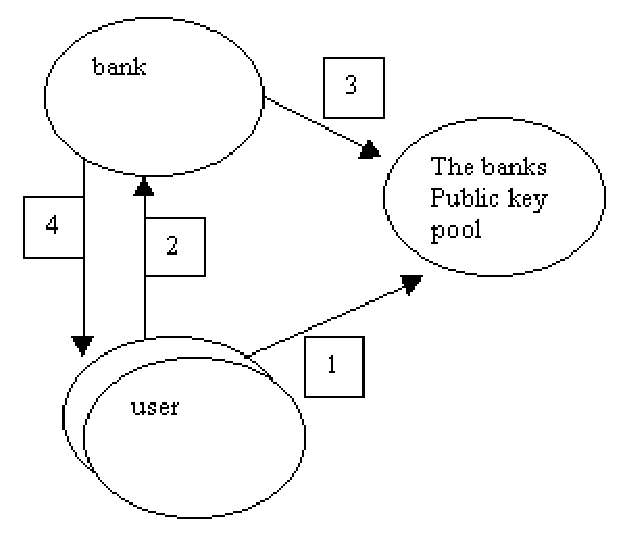
\epsfig{file=pic/cipherRapport.eps}
	\end{center}
	\caption{Key distribution in RSA}
	\label{key distribution}
\end{figure}

\begin{enumerate}
	\item   generate public and private key, send public key to public key 
		directory.
	\item	send a message to the bank saying key available (not encrypted),
		(The user can also send an 'decrypted' message using its
		private key to authenticate that the user is who the user 
		clames he/she is).
	\item	generate public and private key mapped to the particular user. 
		Get users public key and send an encrypted message back using 
		users public key. Then send the public key mapped to the user,
		to the public key pool
	\item	user decrypts message with its private key, and gets the bank's
		public key so it can send encrypted messages to the bank.
\end{enumerate}

In a public key system the keys should be shifted frequently for increased security. 
RSA Inc posts competitions to decipher messages and to current date the best effort 
was made by a team of researchers which managed to break the cipher 
in seven months(!) using a supercomputer. This does not pose as big a threat
as it looks like because the system can be used to agree on a common key
for further use. This key is normaly changed each time a new connection
is established. That means there is very little data for any crypto analysts
to work on deciphering the RSA cipher.

A more important threat to todays internet banking is the future of quantum 
computers. They will be able to solv NP hard problems in polynominal time. The
first quantum-algorithm found is one that can
be used to decrypt just this system.

Remember that changing keys form time to time gives any cryptoanalysts (hackers)
less information and more unreliable 
information as the cryptoanalysts can not know when the cipher key has been changed. 

The RSA cipher is such that deducting the private key from the public is a NP 
hard problem. This means that as the number of digits used for the key are 
increased linearly, the time taken by today's computers increase exponentially,
ciphers with keys of 512 digits are used giving numbers in the range of 
0 .. $ 2^{512} - 1 $ in twos compliment arithmetic.  

\subsection{The class P and NP}

P is the class of algorithms that run in polynomial time. That is, they 
are deterministic.
NP is the class of algorithms that run in exponential time. That is, 
they are non-deterministic. Visualise a binary tree, the more
levels you add to the tree the time taken to visit each level is going
to grow exponentialy.

$ P \subset NP $ as any $P$ problem can be described with a 
decision at each step of one (deterministic choice).

To describe why it is an $NP$ hard problem to deduct the private key from the public 
key we need to understand that it is easy to generate large prime numbers but 
difficult to factor the product of two large prime numbers. We will now introduce 
some new ideas to better understand the RSA public key cryptosystem.
 

\subsection{Modulus}
$a\; mod\; n = b $, $n \ne 0$ has a solution such that $b \in [0, n-1]$.
$b$ is the remainder in integer division $a / n$, and $a = b + k \times n$ for some $k$, 
and $k$ is the product(?) of integer division $a / n$.

%\settabs \+$1$\qquad & three\quad & seventh\cr
%\+$1$&one&first\cr

%\begin{tabbing}
%{hsize = 6in \settabs 2 \columns
%\+Eg 			&$17\; mod\; 12 = 5$ \cr
%\+remainder		&$17 / 5 = 2$ \cr
%\+integer division	&$17 / 5 = 3$ \cr
%We take the lower bound, this can also be written as \newline 
%\+			&$17 / 5 = 3$ \cr
%\+So			&$a = b + k \times n = 2 + 3 \times 5 = 17$ \cr}
%\end{tabbing}

\begin{tabular}{l @{\indent} l}
Eg 		&	\quad$17\; mod\; 12 = 5$ \\
remainder 	&	\quad$17 / 5 = 2$ \\
integer division &  	\quad$17 / 5 = 3$ \\
We take the lower bound, which is written:  
		&	\quad $\lfloor 17 / 5 \rfloor = 3$ \\
So 		&	\quad$a = b + k \times n = 2 + 3 \times 5 = 17$ \\
\end{tabular}

\subsection{Inverse of modulus}
Unlike ordinary arithmetic, modular arithmetic sometimes has inverses. 
We find inverses when solving equations of the form 
$a \times x\; mod\; n = b, n > 0, a \in 0 .. n-1,  x \in 0 .. n-1$
This equation may have $0, 1$ or many solutions, hence inverses.

The greatest common divisor function defined recursively as 
$gcd(a, n) = gcd(n, a\; mod\; n)$ is used to determine the existence of inverses.


\begin{itemize}
\item If $gcd(a, n) = 1$ then, $a \times i\; mod\; n \neq a \times j\; mod\; n, 0 \leq i < j < n$
\item If $gcd(a,n) = 1$ then $a^{-1}$ exists such that $a^{-1} \in [0, n-1]$ and
$a \times a^{-1}\; mod\; n = 1 $
\end{itemize}

Eg. Find the inverse $x$ given the equation $a \times x\; mod\; n = 1$\newline
\indent and $a = 3, n = 7$
\begin{enumerate}
\item $gcd(3, 7) = 1 \Rightarrow$ there exists an inverse.
\item $3 \times i\; mod\; 7 = \{0, 3, 6, 2, 5, 1, 4\}$ where 
		  $i = \{0, 1, 2, 3, 4, 5, 6\}$ \newline
We see that $\{0, 3, 6, 2, 5, 1, 4\}$ is a permutation of $i = \{0, 1, 2, 3, 4, 5, 6\}$. 
This is not true if $gcd(a, n) \ne 1$.

If $a = 3$ and $n = 6$ then $gcd(3, 6) = 3$ and we see that \newline
$3 \times i\; mod\; 6 = \{0, 3, 0, 3, 0, 3\}$ where
	    $i = \{0, 1, 2, 3, 4, 5\}$
does not have an inverse.

By seeing what value $i$ holds when $3 \times i\; mod\; 7 = 1$ we find the inverse $a^{-1}$. 
We see that $i = x = a^{-1} = 5$.
\end{enumerate}

To solve an equation of the form $a \times x\; mod\; n = b$ we need to use what we
know about inverses. The complete set of recidues modulo 10 is: \newline
	$\{0, 1, 2, 3, 4, 5, 6, 7, 8, 9\} = r$. \newline
The reduced set of recidues is $\{1, 3, 7, 9\}$. These elements hold the property that 
they are relatively prime to $n$, in this case $n = 10$. That is, $gcd( r_i, n) = 1$, 
where $i \in [0, n-1]$. Euler's phi function, $\varphi(n)$ gives the cardinality 
of the reduced set of residues. To solve a modular linear equation 
like $35x\; mod\; 50 = 10$ we first find $gcd(35, 50)$:

\begin{table}
	\caption{iteration of {\it extended gcd}}
	\label{gcd1}
	\begin{tabular}{c @{\indent} r r r @{\indent} @{\vrule width 3pt} r r r}
Iteration &  a & b & a/b \qquad & \qquad x' & y' & d \\
\hline 1 & 50 & 35 & 1  \qquad & \qquad  -2 &  3 & 5 \\
2 & 35 & 15 & 2  \qquad & \qquad   1 & -2 & 5 \\
3 & 15 & 5 &  3  \qquad & \qquad   0 &  1 & 5 \\
4 &  5 & 0 & --  \qquad & \qquad   1 & 	0 \\ 
	\end{tabular}
\end{table}


Compute left-hand side of table first, top down. Then use the result to compute
right-hand side of table bottom up. Remember 
	$\lfloor a / b \rfloor$
is integer division taking the lower boundary.

\begin{table}
	\caption{Elaborate explanation of {\it extended gcd}}
	\label{gcd2}
\bigskip
\begin{tabular}{| c | p{2.2in} |}
\hline $gcd(50, 35)$ & 				\leftline{ $i = 4, x' = 1, y' = 0$}
					     	$gcd(5, 0) = 5 \times 1 + 0 \times 0 = 5$ \\
\hline $gcd(35, 50\; mod\; 35) = gcd(35, 15)$ &	\leftline{ $i = 3, x' = 0, y' = 1 - 3 \times 0$}
						$gcd(15, 5) = 15 \times 0 + 5 \times 1 = 5$ \\
\hline $gcd(15, 35\; mod\; 15) = gcd(15, 5)$ &	\leftline{$i = 2, x' = 1, y' = 0 - 2 \times 1$}
						$gcd(35, 15)  = 1 \times 5 - 2 \times 15 = 5$ \\
\hline $gcd(5, 15\; mod\; 5) = gcd(5, 0) = 5$ &	\leftline{$i = 1, x' = -2, y' = -1 - 1 \times (-2)$}
						$gcd(50, 35) = 50 \times -2 + 35 \times 3 = 5$ \\
\hline
	\end{tabular}
\bigskip
\end{table}

We have that $gcd(a, b) = ax' + by' = d$
$x'$ and $y'$ are computed as follows: $x'_i = y'_i + 1, y'_i = 
	x'_i - 1 - \lfloor a_i / b_i \rfloor \times y'_i - 1$
$x'$ and $y'$ are obtained by:\newline
\leftline{$Extended-Euclid(a,\; b)$}
	\leftline{\indent - $if\; b = 0$}
		\leftline{\indent\indent - -$return (a,\; 1,\; 0)$}
	\leftline{\indent - $(d',\; x',\; y') \leftarrow 
			Extended-Euclid(b,\; a\; mod\; b)$}
	\leftline{\indent - $(d,\; x,\; y) \leftarrow d',\; y',\; x' - 
			\lfloor a / b \rfloor \times y'$}
	\leftline{\indent - $return (d, x, y)$}
\begin{itemize}
\item $a \times x\; mod\; n = b$ has $d$ solutions where $d = gcd(a, b)$ or no solutions
\item Let $d = gcd(a, n)$ and suppose $d = a \times x' + n \times y'$ for some integers $x'$ and $y'$. 
If $d | b$ ($d$ divides $b$) then the equation $a \times x\; mod\; n = b$ has one of its solutions $x_0$,
$x_0 = x'(b / d)\; mod\; n$
\end{itemize}
so $x_0 = -2(10/5)\; mod\; 50 = -4\; mod\; 50 = 46 $, 
and the rest of the solutions can be described with  $ x_i = x_0 + i(n / d) $ for 
$i = 1, 2, ..., d-1$

The solutions needs to be in the range $ x_i \in [1, n] $
This gives us:
$x_1 = 6, x_2 = 16, x_3 = 26, x_4 = 36, x_0 = 46 $
This is indeed, d = 5, solutions. \newline
We test the results $x_0$ and $x_1$: \newline
\leftline{\indent $46 \times 35\; mod\; 50 = 1610\; mod\; 50 = 10$}
\leftline{\indent $6 \times 35\; mod\; 50 = 210\; mod\; 50$}

We know from:
\begin{itemize}
\item Euler's theorem states that $n > 1 ,\; p^{\;\varphi(n)} \; mod\; p = 1$
\item Fermat's theorem states that if $p$ is a prime which implies $gcd(a, p) = 1 $
then $a^{p - 1}\; mod\; p = 1$
\end{itemize}


\begin{table}
Finding inverses in modular arithmetic can take very long time.
\caption{modular exponensiation with and without two relative primes}
\label{exponsiation}
\begin{tabular}{l @{\indent}c c c c c c c c c c}
$3^i\; mod\; 7$:	&	1 & 3 & 2 & 6 & 4 & 5 & 1 & 3 & 2 & 6 \\
\hline
i		&	0 & 1 & 2 & 3 & 4 & 5 & 6 & 7 & 8 & 9 \\
$2^i\; mod\; 7$:	&	1 & 2 & 4 & 1 & 2 & 4 & 1 & 2 & 4 & 1 \\
\hline
i		& 	0 & 1 & 2 & 3 & 4 & 5 & 6 & 7 & 8 & 9 \\
\end{tabular}
\newline See how a pattern is created with the value 2.
\end{table}




\chapter{The Cipher Development}

\section{Structure}

The cipher development is composed of two machine specifications, 
{\it Cipher} and {\it Arithmetic}. {\it Arithmetic} 
specifies the exponent ({\it exp}) function ($a^b$), and then it is refined directly 
into an implementation. It is used within the cipher development (introduced in 
the refinement of {\it Cipher}).

{\it Cipher} is very abstract and only says that there exists
operations to decrypt and encrypt a message, and that these
functions together are symmetric. This machine may then be refined into any cipher
like the Caesar shift cipher and the Vigen'ere cipher which make use
of symmetric ciphers and a key, or the RSA cipher which have asymmetric 
ciphers to decrypt and encrypt.
 
This refinement refines the abstract cipher into an exponential cipher by using
the {\it exp} function to define the exact encryption and decryption formulas.
It can be refined into an RSA cipher with small changes to 
the refinement and a little more complications in the proof of its correctness. 
Where we have 
	$$e \times d\; mod\; n-1 = 1 \eqno (1)$$
 in the exponential cipher we would have in 
	$$e \times d=1+k(p-1)(q-1) \eqno (2)$$
in the RSA cipher. $\varphi(n)= (p-1)(q-1)$ where $p$ and $q$ are primes and 
$k= \lfloor a / n \rfloor$ (see section 4.3.1).
(1) states that $e \times d$ must be relative prime to $n$,
and (2) states that $(p-1)(q-1)$ must be relativ prime to $n$.

In the exponential cipher $e$ and $d$ are used to encrypt and decrypt. 
Whiles the RSA makes use of the product of $p$ and $q$ to encrypt
and the prime numbers are used to decrypt. The security of the RSA 
cipher rests on the fact that multiplying two large prime numbers is a one 
way function. It is easy to find the product of two prime numbers but 
difficult (NP hard) to factor a large number to find the two primes. 

The exponential cipher is then implemented. 
Interfaces are used to provide a non-Motif 
execution environment for the two implementations. See chapter 6 for more detail.

\begin{tabular}{c c}
Arithmetic.mch  & Cipher.mch \\
$\downarrow$ & $\downarrow$ \\
& ExponentialCipherRef.ref \\
& $\downarrow$ \\
ArithmeticI.imp & ExponentialCipherI.imp
\end{tabular}


\section{The Arithmetic Machine development}

{\it Arithmetic} functions as a library machine for the
cipher refinement. The need for it may be argued. The ANSII C library
already presents an {\it exp} function. This function is well tested and may prove
to be more efficient than the one specified here. Unfortunately there are
no mechanisms in the BToolkit to import C-library function. This may be 
something the B-Core can extend its toolkit do to in the future. The reason for 
doing it in this project is well justified though, without this constraint. The
development is an exercise in implementing a specification using a 
b-loop construct. Loop constructs in B requires an INVARAINT heading which
is a linking invariant to the refining specificaiton.
It adds a level of difficulty to implementations in B.

The machine introduces a function in the CONSTRAINTS heading
	$$exp \in \nat \times \nat \pfun \nat$$ 
and it is a partial function because exp(0,0) is not defined.
An operation {\it exp\_op} calls this function and returns the value of 
exponentiation, not yet defined.

\vtop{
The specification gives rise to 2 proof obligations: 
\begin{enumerate}
%\item
%$\forall (ff,gg).(ff \in \natone \wedge gg \in \natone \Rightarrow 
%	gcd(ff, gg) = gcd(ff, ff\; mod\; gg))) \wedge \newline
%	\forall ff.(ff \in \natone \Rightarrow gcd(ff, 0) = ff) \wedge \newline
%	gcd(0, 0) = 0 $
\item 
	$\exists prime.(prime \subseteq \nat)$ \newline 
this is trivial. We might prove this by example by saying \newline
	$\{3\} \in prime$ \newline
but unfortunately the BToolProver has no way of deducting that \newline
$\{3\} \in prime \Rightarrow \exists prime.(prime \subseteq \nat)$ \newline
so we have to add the trivial rule: \newline
$\exists p.(p \subseteq \nat)$
\item 
	$\exists exp.(exp \in \nat \times \nat \pfun \nat \wedge \newline
	\forall(aa, bb).(aa \in \nat \wedge bb \in \natone \Rightarrow \newline 
	exp(aa, bb) = exp(aa, bb-1) \times aa \wedge 
	exp(bb, 0) = 1 \wedge exp(0, bb) = 0 ))$ \newline
This is saying that there exists an $exp$ function and that it is defined recursively
as 
	$$exp(aa, bb) = exp(aa, bb-1) \times aa$$
This we know and it is given in the specification.
\end{enumerate}

In general, to prove the existents of a function you can give an example of a 
value for the domain and range of the function.
}

\vtop{
The implementation is given by the b-loop construct: 

\bsetindent
\begin{tabbing}
\bSetTabs
%
%%%%%%%%%%%%%%%%%%%%%%%%%%%%%%%%%%%%%%%%%%  IMPLEMENTATION
%

%%%%%%%%%%%%%%%%%%%%%%%%%%%%%%%%%%%%%%%%%%  OPERATIONS
%
{\bf OPERATIONS} \+ \bbnl

%
%%%%%%%%%%%%%%%%%%%%%%%%%%%%%%%%%%%%%%%%%%  OPERATION exp\_op
%
{\em rr\/} $\longleftarrow$  {\bf { exp\_op}} ( {\em aa\/} , {\em bb\/} ) \bhsp $\defs$ \+ \bnl
 \bOpnWord{IF} \+{\em aa\/} $\neq$ {\em 0\/} $\vee$
{\em bb\/} $\neq$ {\em 0\/} \- \bhsp \bOpnWord{THEN} \+\bnl
\bOpnWord{VAR} \+\bnl
{\em ii\/} , \bnl
{\em kk\/} \-\bnl
\bOpnWord{IN} \+\bnl
{\em ii\/} $:=$  {\em bb\/} \bStatementSemiColon \bnl
{\em kk\/} $:=$  {\em 1\/} \bStatementSemiColon \bnl
\bOpnWord{WHILE} \+\bnl
{\em ii\/} $\neq$ {\em 0\/} \-\bnl
\bOpnWord{DO} \+\bnl
{\em kk\/} $:=$  {\em kk\/} $\times$ {\em aa\/} \bStatementSemiColon \bnl
{\em ii\/} $:=$  {\em ii\/} $-$ {\em 1\/} \-\bnl
\bOpnWord{INVARIANT} \+\bnl
{\em ii\/} $\in$  $\nat$  $\wedge$ \bnl
{\em kk\/} $=$ {\em exp\/}\label{exp}\index{exp}  ( {\em aa\/} , {\em bb\/} $-$ {\em ii\/} )  \-\bnl
\bOpnWord{VARIANT} \+\bnl
{\em ii\/} \-\bnl
\bOpnWord{END}  \bStatementSemiColon \bnl
{\em rr\/} $:=$  {\em kk\/} \-\bnl
\bOpnWord{END}  \-\bnl
\bOpnWord{END}  \-
\end{tabbing}
\bresetindent
%
The invariant states that $ii$ should never be less than 0, and
that the current value of \hbox {$kk = exp(aa, bb-ii)$}. This 
is true as it corresponds to the quantification of {\it exp} given 
in the specification. It is the linking invariant.
}

Execution of {\it Arithmetic}\newline
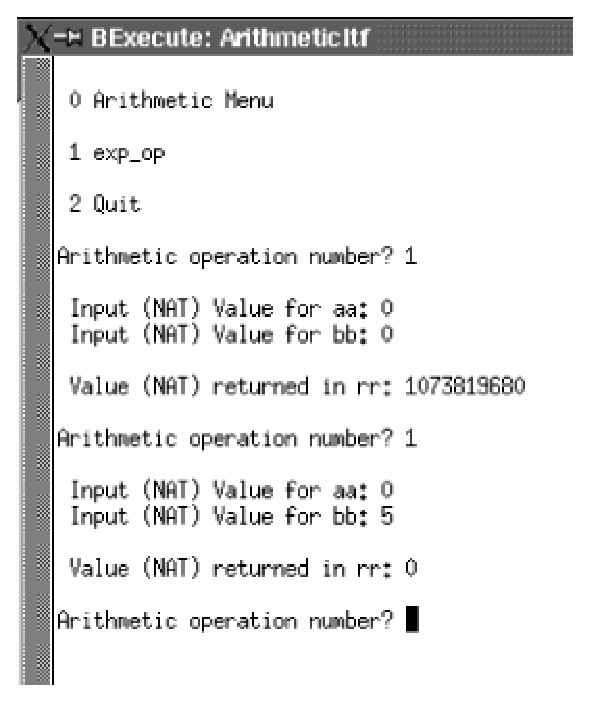
\epsfig{file=pic/Arithmetic_non_motif.eps}

This implementation gives rise to 13 proof obligations. There are 6 proof obligations
which are automatically discharged by the autoprover and can 
therefore be assumed to be trivial. We will have another look at the 
remaining 7 proof obligation and we will see that some of them also are trivial.
There are 11 proof obligations related to the {\it exp\_op} operation, 5 which have
not been discharged by the BToolkit and which we will have a closer look at.
\begin{enumerate}

\item 
	$cst(ArithmeticI\$1) \wedge \newline
	ctx(ArithmeticI\$1) \wedge \newline
	inv(ArithmeticI\$1) \wedge \newline
	asn(ArithmeticI\$1) \wedge \newline
	pre(exp\_op) \Rightarrow \newline
		aa \neq 0 \; \wedge \; \newline
		ii \in NAT \; \wedge \; \newline
		kk \;=\; exp(aa,\; bb-ii) \; \wedge \; \newline
		ii \neq 0 \newline
	\Rightarrow kk \times aa = exp(aa, bb-(ii-1)))$ \newline
This can easily be proven by adding the substitution rule:
$$aa \in \nat \Rightarrow (aa^b) \times aa == aa^{b+1}$$
This proof can be found in appendix A1, Proofs for Arithmetic.imp. 
Notice that the user defined theory introduces variable $aa$ but uses 
a joker, $b$ aswell in the rewrite rule. There is a significant difference 
between these two symboles because $b$ can be anything.

\item 
	... $\wedge\; pre(exp\_op) \Rightarrow \newline
		aa \neq 0 \Rightarrow \newline
	1 \;=\; exp(aa, bb-bb)$ \newline
This is is defined in the specification of $exp$. So 
a user defined theory $aa \in \natone \Rightarrow 1 = exp(aa, 0)$ is added.

\item 
	... $\wedge\; pre(exp\_op) \Rightarrow \newline
		bb \neq 0 \; \wedge \; \newline
		ii \in \nat \; \wedge \; \newline
		kk \;=\; exp(aa,\; bb-ii) \; \wedge \; \newline
		ii \neq 0 \Rightarrow \newline
	kk \times aa \;=\; exp(aa, bb-(ii-1)) $\newline
It can be proven with what we already know and by using the user defined theory
$(aa^b) \times aa == aa^{b+1}$, where $aa \in \nat$. 

\item
	... $\wedge\; pre(exp\_op) \Rightarrow \newline
		bb \neq 0 \Rightarrow \newline
	1 = exp(aa,\; bb-bb)$ \newline
This proof obligation can not be proven. It looks
like we can use the user theory $aa \in \natone \Rightarrow 1 = exp(aa, 0)$,
but we can not because that does not cover the case where $aa = 0$,
and we can not change this because we can not violate the property
that $exp(0, 0)$ does not exist.
If $aa \neq 0$ then we can say \newline
 $ bb \in \natone \Rightarrow exp(aa, bb-bb) = 1 $ \newline
but if $aa = 0$ then we must say
 $ bb \in \natone \Rightarrow exp(aa, bb-bb) = 0 $ \newline
\item
	... $\wedge\; pre(exp\_op) \Rightarrow \newline
		aa = 0 \wedge \newline
		bb = 0 \wedge  \newline
	rrZ = exp(aa,\; bb)$ \newline
This can neither be proven. There is no value for $exp(0,0)$, but the
BToolkit insists that there must be some value for it.

\end{enumerate}

There are 2 proof obligations related to the context of the implementation.
These are the same as for {\it Arithmetic} and have been discussed
above.

\section{Proof of the Exponential Cipher Refinement}

The final cipher development is the result of many other
specifications that have failed or have been dead ends because
they have not resulted in the right proof obligation.
For example in the first attempt of specifying a cipher machine, {\it encrypt\_op}
and {\it decrypt\_op} was defined inside the operations clause and functions
encrypt and decrypt where defined in the invariant:
%%%%%%%%%%%%%%%%%%%%%%%%%%%%%%%%%%%%%%%%%%  CipherB.mch.tex
%
\bsetindent
\begin{tabbing}
\bSetTabs
%
%%%%%%%%%%%%%%%%%%%%%%%%%%%%%%%%%%%%%%%%%%  MACHINE
%
\bbnl
{\bf MACHINE} \bhsp\+{\em CipherB\/} ( {\em ee\/} , {\em dd\/} , {\em nn\/} )  \-\label{CipherB}\index{CipherB}
%
%%%%%%%%%%%%%%%%%%%%%%%%%%%%%%%%%%%%%%%%%%  CONSTRAINTS
%
\bbnl
{\bf CONSTRAINTS} \+ \bbnl
{\em ee\/} $\in$  $\nat$  $\wedge$ \bnl
{\em dd\/} $\in$  $\nat$  $\wedge$ \bnl
{\em nn\/} $\in$  $\nat\bsub{1}$  $\wedge$ \bnl
{\em ee\/} $\times$ {\em dd\/} \ {\sf mod}\ {\em nn\/} $-$ {\em 1\/} $=$ {\em 1\/} \-
%
%%%%%%%%%%%%%%%%%%%%%%%%%%%%%%%%%%%%%%%%%%  VARIABLES
%
\bbnl
{\bf VARIABLES} \+ \bbnl
{\em encrypt\/}\label{encrypt}\index{encrypt}  , {\em decrypt\/}\label{decrypt}\index{decrypt}  \-
%
%%%%%%%%%%%%%%%%%%%%%%%%%%%%%%%%%%%%%%%%%%  INVARIANT
%
\bbnl
{\bf INVARIANT} \+ \bbnl
{\em encrypt\/} $\in$  $\nat$  $\fun$  $\nat$  $\wedge$ \bnl
{\em decrypt\/} $\in$  $\nat$  $\fun$  $\nat$  $\wedge$ \bnl
$\forall$ {\em mm\/} . ( {\em mm\/} $\in$ {\em 0\/} $\upto$ {\em nn\/} $-$ {\em 1\/} $\Rightarrow$
{\em encrypt\/} ( {\em decrypt\/} ( {\em mm\/} )  )  $=$ {\em mm\/} ) $\wedge$ \bnl
$\forall$ {\em mm\/} . ( {\em mm\/} $\in$ {\em 0\/} $\upto$ {\em nn\/} $-$ {\em 1\/} $\Rightarrow$
{\em decrypt\/} ( {\em encrypt\/} ( {\em mm\/} )  )  $=$ {\em mm\/} ) \-
%
%%%%%%%%%%%%%%%%%%%%%%%%%%%%%%%%%%%%%%%%%%  OPERATIONS
%
\bnl\bnl
{\bf OPERATIONS} \+ \bbnl

%
%%%%%%%%%%%%%%%%%%%%%%%%%%%%%%%%%%%%%%%%%%  OPERATION encrypt\_op
%
{\em rr\/} $\longleftarrow$  {\bf { encrypt\_op}} ( {\em mm\/} ) \bhsp $\defs$ \+ \bnl
 \bOpnWord{PRE} \+\bnl
{\em mm\/} $\in$ {\em 0\/} $\upto$ {\em nn\/} $-$ {\em 1\/} \-\bnl
\bOpnWord{THEN} \+\bnl
{\em rr\/} $:=$  {\em encrypt\/} ( {\em mm\/} )  \-\bnl
\bOpnWord{END}  \-\- \bbnl

%
%%%%%%%%%%%%%%%%%%%%%%%%%%%%%%%%%%%%%%%%%%  END
%
\bbnl
{\bf END} 
\end{tabbing}
\bresetindent

This generates proof obligation
$$(P \wedge Q \wedge R \wedge L) \Rightarrow [S]R $$
for the operation {\it encrypt\_op}. With this development we wishe to prove
the $encrypt(decrypt(mm)) = mm$. That is, the cipher is symmetric.

The first proof obligation of the internal consistency of a 
machine is generated by \newline
$\exists x.P $ \newline %number these lines!!!
and it says if P are the constraints on the parameter of the machine, then
there should be some values of the parameter $x$ that meet this constraints.
{\it Cipher} has constraints: \newline
CONSTRAINTS \newline
\indent	$ee \in \nat \wedge$ \newline
\indent	$dd \in \nat \wedge$ \newline
\indent	$nn \in \natone \wedge$ \newline
\indent	$ee \times dd\; mod\; nn-1 = 1$ \newline
and the proof obligation generated says 
$$\exists(ee,dd,nn).(ee\in \nat \wedge dd\in \nat \wedge nn \in \natone 
	\wedge ee \times dd\; mod\; nn-1 = 1)$$
This can be proven by example given:
$$ee=5,dd=5,nn=5 \Rightarrow (ee\in \nat \wedge dd \in \nat \wedge nn \in \natone
	 \wedge ee \times dd\; mod\; nn-1 = 1)$$

If we look at the proof obligation for PROPERTIES \newline
$P \Rightarrow \exists y.Q $ \newline
It says that there are constants y that meet the PROPERTIES clause
Q provided they meet the constraints P. This gives the proof obligation we are
looking for.

In the final cipher specification, functions {\it encrypt} and {\it decrypt} 
are defined under the CONSTANTS clause and then the operations 
{\it encrypt\_op} and {\it decrypt\_op} simply returns the result of calling 
these fuctions. This generates proof obligation {\it encrypt(decrypt(mm)) = mm}.
It is a common way of defining operations in B, and has also been
applied in the arithmetic machine to define exp. It results in  
proof obligation\newline
$P \Rightarrow \exists y.Q $ \newline
and is an easier proof than $\exists x.P $ 

The exponential cipher was introduced in last section. Here we will provide a 
proof of its correctness. It is worth noticing that {\it binhyp} is a way of
introduing variables that only appares on the rigth hand of a substitution rule.

Choose $n$, $e$, $d$ so that $n$ is prime, $gcd(n, e) = 1$, and $e \times d\; mod\; 
		\varphi(n) = 1$ 
$$ E(m) = m^e\; mod\; n, m \in [0, n-1] $$
$$ D(m) = m^d\; mod\; n $$ 
Then we must show that $D(E(m)) = m$ \newline
After applying the DED (deduction) rule we have the following expression in
the BToolkit\newline
$\exists(encrypt,decrypt).(encrypt \in \nat \fun \nat \wedge decrypt 
\in \nat \fun \nat \wedge \forall mm.(mm : 0..nn-1 \Rightarrow 
	encrypt(decrypt(mm)) = mm) \wedge
\forall .mm.(mm \in 0..nn-1 \Rightarrow decrypt(encrypt(mm) = mm))$ \newline
Then we apply a rewrite rule to substitute {\it encrypt(mm)} and {\it decrypt(mm)}
with their respectiv functions. So one rewrite rule say: \newline
$binhyp(n \in \natone) \wedge \newline 
binhyp(e \in \nat) \Rightarrow \newline 
encrypt(x) == exp(x, e)\; mod\; n$ 

\begin{tabular}{p{2.2in} p{2.2in}}
So $ D(E(m))$ &	$= (m^e\; mod\; n)^d\; mod\; n$ \\
&		$= (m^e)^d\; mod\; n$ \\
&		$= m^{e \times d}\; mod\; n$ \\
\multicolumn{2}{p{4in}}{
from $e \times d\; mod\; \varphi(n) = 1$ we know that 
	$e \times d = K \times \varphi(n) +1$ for some $K$
from the definition of modulus. \newline
The BToolUserheory.5 states: \newline
$e \in \nat \newline
d \in \nat \newline
binhyp(n \in \natone) \newline
e \times d\; mod\; n-1 = 1 \newline
k \in \natone \newline
\Rightarrow \newline
e \times d == k \times (n-1)+1$} \\
&		$= m^{k \times \varphi(n) + 1}\; mod\; n $ \\
&		$= m^{k \times \varphi(n)} \times m\; mod\; n $ \\
&		$= (m^{k \times \varphi(n)}\; mod\; n) \times m\; mod\; n $ \\
&		$= ((m^{\varphi(n)}\; mod\; n)^k) \times m\; mod\; n $ \\
\multicolumn{2}{l}{
Eulers theorem states that $a^{\varphi(n)}\; mod\; n = 1$} \\
&		$= 1^k \times m\; mod\; n $ \\
&		$= m\; mod\; n$ \\
$m \in [0,n-1] \Rightarrow m\; mod\; n = m $ \\
\end{tabular}

The complete proof print can be found in 
Appendix A1, Proofs for ExponentialCipherRef.ref, together with
all the added rewrite rules and the order in which they have been applied. 
Note that the second part of the symmetry proof has been galantly skiped over
by adding a simple substitution rule. This is because the proof file became 
so big that the BToolkit was not able to generate a marked up latex file from it
as can be seen from the picture.

\epsfig{file=pic/no_proof_print_cipher.eps}

\subsection{Some Issues About the BToolUserTheories and the exponential cipher proof}

In the Appendix A1, Proofs for ExponentialCipherRef.ref, 
BToolUserTheory.5 is defined as:
$$e \in \nat \wedge d \in \nat \wedge binhyp(n \in \natone) \wedge k \in \natone 
	\Rightarrow e \times d == k \times (n-1)+1$$
The variable $k$ is introduced with very little restriction. There
is a particular $k$ we are looking for but we do not care
what value it holds as it has no influence on the proof, and 
$k$ is defined as $k= \lfloor a / n \rfloor$. We can not
say $\exists k.(k \in \natone)$ bacause there is a particular $k$.
The way of introduceing $k$ in this rule is not very formal.

Because $k$ is not added to the hypotesis of the 'cipher proof',
we have to add BToolUserTheory.6 which state $k \in \natone$
and BToolUserTheory.8 which is a consequence of the prevoius rule,
$k \in \natone \Rightarrow k \in \nat$. Had $k$ been
added to the hypotesis, at least the last rule would have been
'explored' by the hypotesis environment. Is there a way of adding variables to the
hypotesis of a proof?

BToolUserTheory11 is long-winded but very nessesery to complete the proof,
$$n \in \natone \Rightarrow a \times b\; mod\; n == 
	a \times \;mod\; n \times b\; mod\; n\; mod\; n$$

There should be a way of expressing BToolUserTheory17 more precise. 
It uses a joker $mm$ to substitute
$mm\; mod\; nn = m$. It would be more precise to state: \newline
$$n \in \natone \wedge a \in 0..n-1 \Rightarrow a\; mod\; n == a$$ but there
are no facts about $mm$(!) in the hypothesis so the rule does not 'fire' .

BToolUserTheory18 is there because we have not shown that there exists
function {\it encrypt} and {\it decrypt}. This bit of the proof is a shortcut and 
not formal. The proof consists of two parts,
\begin{enumerate}
\item prove {\it encrypt(decrypt(mm)) = mm }
\item prove {\it decrypt(encrypt(mm)) = mm}
\end{enumerate}
Obiously, these two parts involve the same steps to be proven. For the
reasons described at the end of last sections it has been added
to make the proof shorter.

\section{Benefits of Completing Proof Obligations}

The purpose of completing proof obligations is to say that the
specification models something and is consistent. In proving the
consistency the specifier might discover errors in the specification.
One such flaw that arose in {\it Cipher} is described here.
The PROPERTIES heading initially said: \newline
$ \forall mm.(mm \in \nat \Rightarrow D(E(m)) = m\; \wedge \; E(D(m)) = m) $\newline
this is too strong and should say:\newline
$ \forall mm.(mm \in 0..nn-1 \Rightarrow D(E(m)) = m\; \wedge \; E(D(m)) = m) $\newline
This shows that completing a proof can either make you change the specification
because it is not correct or you find that it does not specify what you
intend it to specify.

\chapter{The ATM Development}

\section{Structure}

This chapter will discuss ideas of how to specify networking in B. It will review 
some awkward restrictions implied by the BToolkit which are too strong.
It will discuss the problems it has resulted in, 
how it has been dealt with, how some models
generalise to other problems found in computer science. 
Finally a discussion is offered as to why
the client-server architecture is not suited for implementation in B.

The reasons for attempting to model something as uncertain as network
communication are many. This development searches to find a model
that both allows the specifier to state some global invariants about
a client-server transaction system and at the same time provide opportunities
to refine the model. Finding a model which both allows for a global invariant
to be proven and which can be refined into working code would be a step forward in
modelling transaction systems in B.

One of the challenges when specifying network communication is that 
the specification can become too abstract as a result of the uncertainty caused
by the network layer or in an attempt in stating some global invariants about
the system. What happens to the the customer's balance if the ATM crashes
just before the customer gets his or her money? What happens with the customer's
balance if the network goes down just after a customer has deposited money? 
There should be invariants in the development to say something about this,
and in particular that "no money is lost over the network layer". 
How can this be achived in B, and can such a specification be implemented?

\section{What the Application Should do}

The attempts to specifying an ATM system has one common component, the 
{\it Bank} provides functionality to create an account,
withdraw and deposit money, query if an account exists, and query the balance
of an account. These operations are basic and they are only there to illustrate 
the network communication. In a more realistic system, access restrictions
would be imposed on the query balance, withdrawal, and deposit operations. 
There would be operations; log on and log off and an operation to delete accounts 
amongst others.


In developments where the ATM has been specified seperately, the specification has 
been very simple. The ATM should idealy only present information to its user.

\section{First Approach}

The first step was to learn about how to construct specifications. In [1] there is 
an airspace specification which makes use of some of the structuring mechanisms 
provided by the BToolkit with the two most important; SEES and INCLUDES.

There was a subtle error in this development that gave a clue to 
a major obstacle which required a different mind set when developing
the ATM system. From previous experience of Java programming, B can be viewed
in some way similar to an object oriented system. Each machine specification
can be viewed as an object, and a machine including another machine
can be seen as an object instantiating another object.
Of course that is almost as far as the similarity goes. 
The B INCLUDES construct demands exclusive access and INCLUDES is used 
in specification. Java is merely a programming language.

The airtraffic development discussed in [1] introduces machines:
{\it Aircraft} which holds a set of aircrafts, {\it Controller} 
relates a controller to
an aircraft, {\it Airspace} defines flight regions like city, 
military and airport zones and provides operation to move aircrafts
between zones. Finally {\it ATCSystem} defines the operation 
{\it hand\_over\_aircraft} needed when an aircraft changes zone. The aircraft 
must be handed over to a new controller and the two zones the 
aircraft flights from and to must be updated.

{\it ATCSystem} promotes an operation from {\it Controller} which
it does not extend but makes use of in {\it hand\_over\_aircraft}. First of all
this is an error, second it can not be solved by extending {\it Controller}. 
If the machine
had extended {\it Controller}, there would be a circular structure where
{\it ATCSystem} includes/extends {\it Airspace} and {\it Controller},
( {\it ATCSystem} $\rightarrow$ ({\it Airspace, Controller})) and {\it Airspace} 
includes {\it Controller},
({\it Airspace} $\rightarrow$ {\it Controller}). Hence there would be two
'instances' of {\it Controller} in {\it ATCSystem} because INCLUDES is defined as:

{\parindent = 12pt \narrower
"INCLUDES: exclusive access; sets and constants of the included machine are
visible in the including; variables of the included machine are visible
in the invariant...;operations of the included can be used in the 
operations of the including;..."\newline
"Extends: as for INCLUDES, ...".
If the operations is to be used in the extending machine they
must be promoted." \par} \parindent = 0pt
	\rightline{([1], p 39)} 

The other constructs like SEES and USES are defined to take shared access
but do not allow operations to be called. \newline \newline

The solution to the problem is to move the call to 
operation {\it add\_aircraft} from {\it Airspace} to {\it ATCSystem}, which will 
both add a new aircraft to a new airspace and assign the aircraft to a new controller.
Then the INCLUDES link between 
{\it Airspace} and {\it Controller} can be broken. A new INCLUDES link between 
{\it ATCSystem} and {\it Controller} must be made. Therefore in {\it ATCSystem} 
we have to redefine both operation {\it add\_aircraft} from {\it Airspace} machine
and {\it transfer\_aircraft} from the {\it Controller} machine. 
The modified specification can be found in Appendix B, the original specification
can be found in [1] (p 44). \newline \newline

\begin{figure}[hbpt]
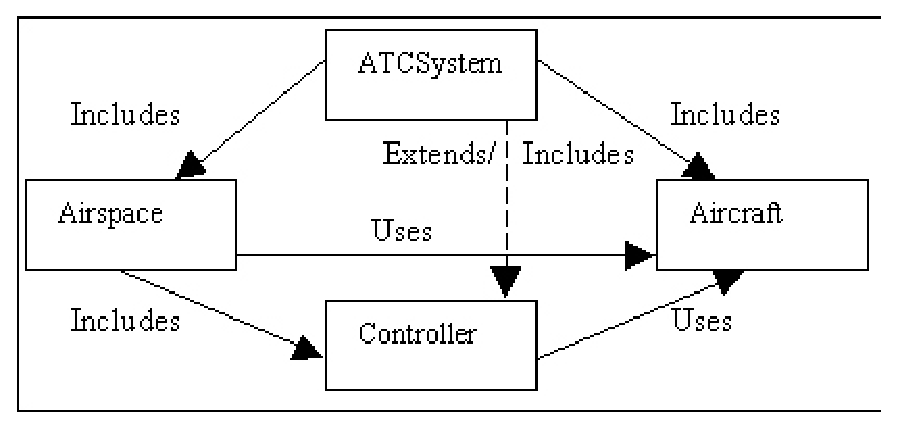
\epsfig{file=pic/atc1.eps}
\caption{Aircraft control system from [1]}
\label{atc1}
\end{figure}


\begin{figure}[hbpt]
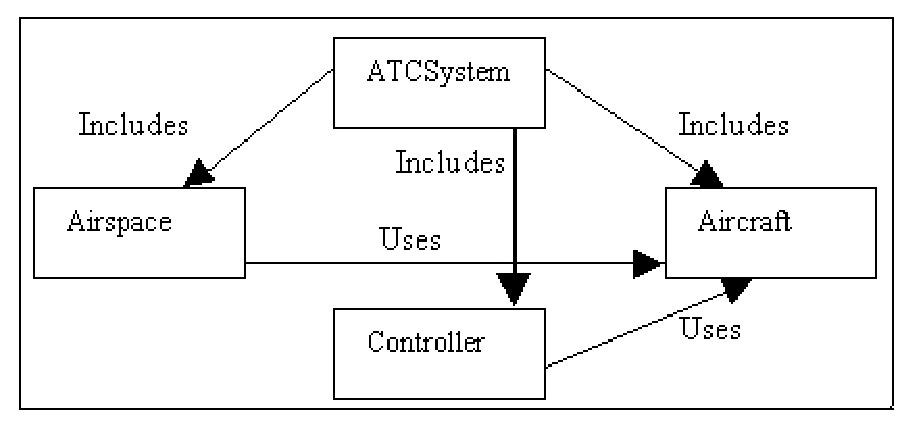
\epsfig{file=pic/atc2.eps}
\caption{modified system}
\end{figure}

\section{A Client-Server Protocol}

The initial attempt was made with a client and server machine and a protocol
specification to connect them. The first issues were to resolve how does
the {\it ATM} machine send messages to the server, and where does the event;
receiving messages happen? Does it happen in {\it ATM} and {\it Bank} or in 
a global protocol machine?

The first problem encountered was that of including machines to allow 
a two way communication. The first specification resulted in a circular
include construct just like that found in the airtraffic control system
\newline\newline

\begin{figure}[h]
	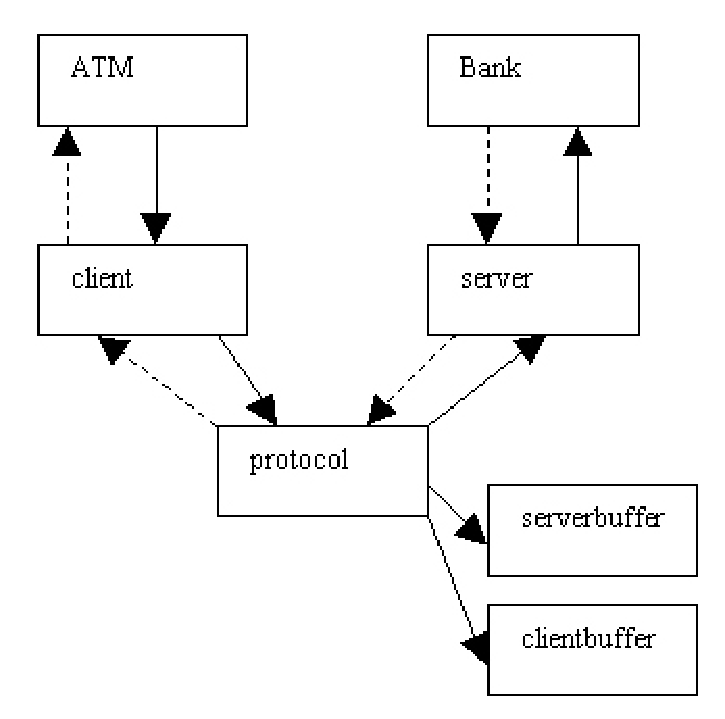
\epsfig{file=pic/protocol.eps}
	\caption{Protocol model for establishing communication, 
		all the arrows denote INCLUDES}
	\label{protocola}
\end{figure}
 
When a user logs on to the ATM it needs to send messages to bank.
So the message must go through the client. The client calls operations on
the protocol machine. First the client request a connection with the server, then
it may request data which the server will forward to the bank, so the server 
must again call operations on the bank.

So far the message has only gone one way. If the bank is to reply to the
message, it must see operations on the server, hence include/extend server.
The server must call operations on protocol and so forth. This is not
allowed, so this approach can only model one-way communication. It is
unfortunate bacause the model has a good prospect of being refined
and global invarinats may be stated in the protocol machine. 

Throughout, these machines are defined as follows:
\begin{itemize}
\item {\it ATM} and {\it Bank} specifies the business logic for the ATM development
\item {\it Client} and {\it Server} establish and maintain a connection. It can
also be extended to preserve session ids for each user loggin on to the ATM.
The {\it Server} can also be extended to allow a "protocol" call mechanism to
the {\it Bank} operations as discussed in section 5.6, Networked Bank
\item The {\it Protocol} has a system view. It holds two buffers,
{\it clientbuffer} and {\it serverbuffer}. These buffers model data
travelling on the network.
\end{itemize}

The next sections discusses different approaches to solving this problem and
making the communication two-way.

Appendix C.1.1 shows how a connection between the server and client
can be established. This builds on the realtime communication protocol
from [1] (p. 135).

Appendix C.1.2 Shows how the communication protocol can be extended to
allow the {\it ATM} and the {\it Bank} to communicate. 

\begin{figure}[h]
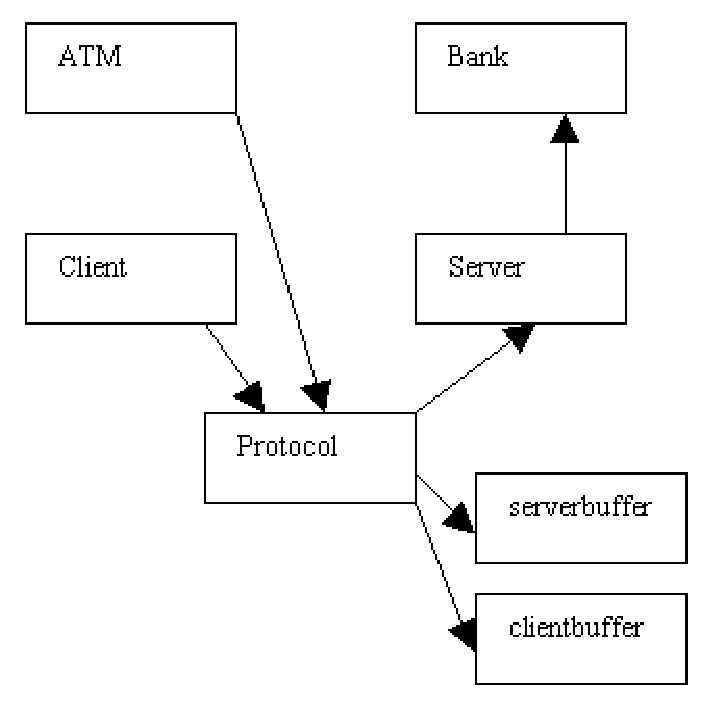
\epsfig{file=pic/protocol2.eps}
\caption{A new model with extensions to the ATM system}
\label{protocola}
\end{figure}

{\it Server} INCLUDES {\it Bank} and {\it ATM} INCLUDES {\it Protocol}.
Both {\it Protocol} and {\it ATM} can be animated to show system functionality.

There is a problem with this approach in that each operation in
{\it Bank} and {\it ATM} must be dupplicated in {\it Protocol} and
in {\it Server}, and
if the {\it ATM} requests an operation from {\it Bank}, it is going
to get the reply via a return value from the opertion in {\it Bank} when
more realisticly it should be stored in a buffer.

Two important answers to consider are:
\begin{enumerate}
	\item How do we refine the development into an implementation? 
	\item Can {\it Protocol} be implemented, and what functionality would it have?
\end{enumerate}

\section{Receiver, Sender and Readers-Writers Problem}

This development has a {\it SecureNetwork} machine which holds data
in a buffer, and two other machines, {\it Receiver} and {\it Sender}, which 
communicate with each other by calling operations {\it receive} and {\it send} on 
{\it SecureNetwork}. These two machines may be refined into an ATM system, and 
the implementation can make use of the {\it SocketServer} and {\it SocketClient} 
library machines. See Appendix C.2
\newline\newline

\begin{figure}[h]
\epsfig{file=pic/secureNetwork.eps}
\caption{secure Network model}
\label{secure network}
\end{figure}


This models the interaction between a client and a server with a buffer held
by {\it SecureNetwork}. 
It can provide the basis for an ATM system that allows for refinement of
the {\it ATM} and {\it Bank} into two seperate implementations.
Can this model refine a buffer specification where both
the {\it ATM} and the {\it Bank} is specified in the same machine?
A solution to this has been added to the last section of this
chapter and the resulting problems will be discussed.

{\it SecureNetwork} holds a sequence of messages. When anyone
sends a message, it is added to the end of the message sequence and
when someone calls {\it receive} they are given the first message in
the sequence.

To distinguish the recipient of a message from other recipients, the
{\it SecureNetwork} may be refined such that the message consists of
a head and a tail. The head identifies to whom
the message is intended for, and the tail consists of the data. The
data must be stored in such a way that anyone can enquire the
heading of a message without "popping" it of the fifo (first in, first out)
sequence. See the data link layer of the OSI model [10] (p 43).
This is the same strategy applied in the LAN (Local Area Network) protocol.
So this model may be extended by making the receiver the {\it Bank}
and by making the sender the {\it ATM}. 

This model may also be seen as modelling the buffered readers-writers problem
like the ones found in database systems or operating systems. Then
the two operations {\it receive} and {\it send} in {\it SecureNetwork}
should be refined into semafores.

The first approach to this model was made with use of
preconditions instead of guards. The operations in SecureNetwork would
then look something like this:

\quad  mm $\leftarrow$ receive = \newline
\quad \quad	PRE 	\newline
\quad \quad \qquad		$card(msg) > 0 $ \newline
\quad \quad	THEN \newline
\quad \quad \quad 	mm := first(msg) \newline
\quad	END 

For a {\it receiver} specification to make use of this operation it would
first have to enquire the {\it SecureNetwork} if it had received any messages
or it would have to be notified by the {\it sender} that it had sent a message.
The first approach is tedious, having to call two operations to receive
a message. The second approach requires a lot of work from the sender
and in addition the sender may not know all the receivers, just as
a datafield in C may not know who is pointing at it, consequently the problem of 
garbage collection.
		
A fictitious model (with fictitious I mean a model with cicular includes constructs)
was made where the {\it Sender} would include {\it SecureNetwork} and {\it Receiver}.
{\it Receiver} included {\it SecureNetwork} and whenever {\it Sender} 
wrote to the buffer in {\it SecureNetwork} it would set a flag 
in {\it Receiver} to say that it had written to the buffer.

\section{Networked Bank}

This is an attempt on only a specificating the server. It builds on the idea
that there is not much to say about the operations of ATM as ATMs only
receive and send data to the server and therefore does not maintain any
data. So hence a specification of the client would mostly use non-deterministic
substitution ($:\in$) to say something about the return value. This is a
diversion on the route to find a model that both satisfies global invariants
and can be refiend. The purpose is to produce two executable B implementations.

The {\it networkedBank} provides an interface for calling the 
operations on the {\it Bank}. Each operation in {\it Bank} is specified 
in {\it NetworkedBank} such that it can be called from any {\it ATM} 
using a protocol. When {\it ATM} calls an operation on {\it NetworkedBank}
it sends a number. This number is stored in a sequence,
{\it creq} for call-request, and each number in {\it creq} is 
associated with an operation  in {\it Bank}. Another sequence {\it ff} holds the 
parameter value(s) to be passed to the operation in {\it Bank}. 

\bsetindent
\begin{tabbing}
\bSetTabs
%
%%%%%%%%%%%%%%%%%%%%%%%%%%%%%%%%%%%%%%%%%%  MACHINE
%
{\bf MACHINE} \bhsp\+{\em NetworkedBank\/} \-\label{NetworkedBank}\index{NetworkedBank}
%
%%%%%%%%%%%%%%%%%%%%%%%%%%%%%%%%%%%%%%%%%%  SEES
%
\bbnl
{\bf SEES} \bhsp{\em Bool\_TYPE\/}\label{Bool_TYPE}\index{Bool_TYPE}
%
%%%%%%%%%%%%%%%%%%%%%%%%%%%%%%%%%%%%%%%%%%  INCLUDES
%
\bbnl
{\bf INCLUDES} \bhsp{\em Bank\/}\label{Bank}\index{Bank}
%
%%%%%%%%%%%%%%%%%%%%%%%%%%%%%%%%%%%%%%%%%%  VARIABLES
%
\bbnl
{\bf VARIABLES} \+ \bbnl
{\em ff\/}\label{ff}\index{ff}  , {\em creq\/}\label{creq}\index{creq}  \-
%
%%%%%%%%%%%%%%%%%%%%%%%%%%%%%%%%%%%%%%%%%%  INVARIANT
%
\bbnl
{\bf INVARIANT} \+ \bbnl
{\em ff\/} $\in$  {\sf seq}$\;$(  $\nat$  )  $\wedge$ \bnl
{\em creq\/} $\in$  {\sf seq}$\;$(  $\nat$  )  $\wedge$ \bnl
{\sf size}$\;$( {\em ff\/} )  $\leq$ {\em maxParams\/} \bnl
... \-
%
%%%%%%%%%%%%%%%%%%%%%%%%%%%%%%%%%%%%%%%%%%  END
%
\bbnl
{\bf END} 
\end{tabbing}
\bresetindent
% 

\begin{figure}[h]
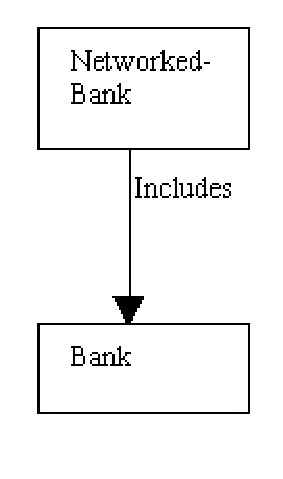
\epsfig{file=pic/networkedBank.eps}
\caption{Wraped bank model}
\label{networked bank}
\end{figure}

Then there is an operation, {\it check\_clientreq}, which takes the last value in 
{\it creq} and compares it with the numbers associated with operations 
in {\it Bank}. If a match is found, the operation is called. The parameter 
values are taken from the {\it ff} sequence. 
{\it check\_clientreq} does not check if the in-parameters from {\it ff} are correctly 
associated with the right operation calls.
It is assumed to be correctly associated with the{\it ATM\_x} operation
(x are operations like {\it create\_account} 
{\it deposit} and any other operation found in {\it Bank} and which 
has been 'promoted' to {\it NetworkedBank}). {\it NetworkedBank}
pushes in-parameter(s) onto {\it ff}, 
and {\it check\_clientreq} pops each element off {\it ff}. Though, this 
is not a proof obligation from the machine, the specification should have 
been expressed in a way to state that each parameter is
correctly associated with an operation call on {\it Bank} even if the
parameters are of the correct type. This is a weakness. 
How may the specification constraine this?
Doing the type checking in {\it check\_clientreq} would be useless
as many of the operations in {\it Bank} take the same type. Hence checking for
type does not guarantee an operation call with the right parameter(s). Also
type checking in {\it NetworkedBank} will generate proof obligation
in any machine which makes use of its operation ({\it ATM)}
without sufficient knowledge to discharge them in thouse machines.

%%%%%%%%%%%%%%%%%%%%%%%%%%%%%%%%%%%%%%%%%%  NetworkedBank.mch.tex
%
\bsetindent
\begin{tabbing}
\bSetTabs
%
%%%%%%%%%%%%%%%%%%%%%%%%%%%%%%%%%%%%%%%%%%  OPERATION check\_clientreq
%
{\em num\/} , {\em ok\/} , {\em op\/} $\longleftarrow$  {\bf { check\_clientreq}}  \bhsp $\defs$ \+ \bnl
 \bOpnWord{IF} \+ {\sf card}$\;$( {\em creq\/} )  $>$ {\em 0\/} \- \bhsp \bOpnWord{THEN} \+\bnl
\bOpnWord{VAR} \+{\em aa\/} , {\em bb\/} \- \bhsp \bOpnWord{IN} \+\bnl
\bOpnWord{IF} \+ {\sf last}$\;$( {\em creq\/} )  $=$ {\em 1\/} \- \bhsp \bOpnWord{THEN} \+\bnl
{\em creq\/} $:=$   {\sf front}$\;$( {\em creq\/} )  \bparallel \bnl
{\em num\/} , {\em ok\/} $\longleftarrow$ {\em create\_account\/}\label{create_account}\index{create_account}  \bparallel \bnl
{\em op\/} $:=$  {\em 1\/} \-\bnl
\bOpnWord{ELSE} \+ \bOpnWord{IF} \+ {\sf last}$\;$( {\em creq\/} )  $=$ {\em 2\/} \- \bhsp \bOpnWord{THEN} \+\bnl
{\em creq\/} $:=$   {\sf front}$\;$( {\em creq\/} )  \bparallel \bnl
{\em aa\/} $:=$  {\em ff\/} (  {\sf card}$\;$( {\em ff\/} )  $-$ {\em 1\/} )  \bparallel \bnl
{\em bb\/} $:=$  {\em ff\/} (  {\sf card}$\;$( {\em ff\/} )  )  \bparallel \bnl
{\em ff\/} $:=$  {\em ff\/} $\uparrow$  {\sf card}$\;$( {\em ff\/} )  $-$ {\em 2\/} \bparallel \bnl
{\em ok\/} , {\em num\/} $\longleftarrow$ {\em deposit\/}\label{deposit}\index{deposit}  ( {\em aa\/} , {\em bb\/} )  \bparallel \bnl
{\em op\/} $:=$  {\em 2\/} \-\bnl
...

\end{tabbing}
\bresetindent
%
%
%\end{tabbing}
\bresetindent
%

The return values are passed back through the 
chain of communication created when the {\it ATM} calls an operation. 
This allows for a two-way communication at the same time as creating 
a top-down include-construct. 

In order to prove the correctness of the specification, the operations in one of
{\it Bank}'s precondition has been changed to a guard. 

create\_account = \newline
\qquad	PRE accountNumber $\neq$ ACCOUNTS THEN \newline
...

has been changed to \newline
create\_account = \newline
\qquad	IF accountNumber /= ACCOUNTS THEN \newline
...

The reason for mentioning this is that a similar change would have to be made 
on the operations {\it withdraw}, {\it isaccount}, and
{\it getbalance} to completely remove all unproved proof obligations in 
{\it NetworkedBank}.
Alternatively this type checking could be forwarded to {\it NetworkedBank}, which
again would be generating proof obligations in ATM. An {\it ATM} machine should
not know about all the types and variables in {\it Bank} and consequently 
there are no possibility of proving it withing {\it ATM}.

\subsection{parallel operations, relational image and sequence concatenation}

In the {\it ATM\_x} operations where in-parameters are required
they must be stored somehow.
In {\it ATM\_deposit} the following was first given: \newline
... \newline
$ff := ff(a) \leftarrow acc$ \bparallel  \newline
$ff := ff(b) \leftarrow amount$ \bparallel \newline
and $ff$ is a sequence. This is legal if $a \neq b$, put does not parse in B.
This is too strong, but we know that  \newline
$ff(a) := x $ \newline
$ff(b) := y $ \newline
is equivelant to  \newline
$ff$ := $ff$ $
	<\kern-.65em\raisebox{.275ex}{$\scriptscriptstyle +$}\;$ 
		\{$a$ $\mapsto$ $x$, $b$ $\mapsto$ $x$\}  \newline
This does the same as the parallel substitution and is allowed in B. 
It can be used as long as the relational override preserves the sequence constraint
that $dom(ff) = 1..size(ff)$ but what if $a = size(ff) + 1$ and
$b = size(ff) + 2$ ?


The only rule in the BToolkit that applies to this expression is
InSequenceX.20 \newline
$binhyp(f \in seq(S)) \wedge \newline
dom(g) \subset dom(f) \wedge \newline
ran(g) \subset S$  \newline
$\Rightarrow$ \newline
$f$ 
	$<\kern-.65em\raisebox{.275ex}{$\scriptscriptstyle +$}\;$ 
		$g$ $\in$ $seq(S)$ 

Applying this rule to
$ff$ 
	$<\kern-.65em\raisebox{.275ex}{$\scriptscriptstyle +$}\;$ 
		\{$a$ $\mapsto$ $x$, $b$ $\mapsto$ $y$\} $\in$ $seq(ff)$ \newline
where $a$ = $card(ff)+1$ and $b$ = $card(ff)+2$ gives \newline
$H$ $\vdash$ $ff$ 
	$<\kern-.65em\raisebox{.275ex}{$\scriptscriptstyle +$}\;$ 
		\{$card(ff)+1$ $\mapsto$ $x$, $card(ff)+2$ $\mapsto$ $y$\} $\in$	 
		$seq(\nat)$ \newline
	\qquad -- $H$ $\vdash$ $ff \in seq(\nat)$ \newline
	\qquad -- $H$ $\vdash$ $dom$(\{$card(ff)+1$ $\mapsto$ $x$, $card(ff)+2$ $\mapsto$ $y$\}) 
			$\in$ $seq(\nat)$ \newline
...\newline
It can not bee proven that \newline
$dom$(\{$card(ff)+1$ $\mapsto$ $x$, $card(ff)+2$ $\mapsto$ $y$\}) 
			$\in$ $seq(\nat)$ \newline
The proof rule InSequenceX.20 is true, but too strong for this
proof obligation as the hypotheses \newline
	$dom(g) \subset dom(f)$ \newline
is false for this relational override
and it does not allow a sequence to grow. \newline

\vtop{
Definition of relational over-ride:\newline
{\parindent = 12pt \narrower 
"if $R_0 \in s \rel T$ and $R_1 \in s \rel T$ are two relations between
$s$ and $t$, then the relational over-ride $R_0$ 
	$<\kern-.65em\raisebox{.275ex}{$\scriptscriptstyle +$}\;$ 
					 $R_1$ is the relation $R_0$
with certain relationships replaced by those in $R_1$. This amounts to
the relation $R_1$ together with any reminding relationships that $R_0$ has which are
outside the {\bf domain of $R_1$}." \par} \parindent = 0pt
	\rightline{([2], p 79)}
}

Therefore $ff := ff $
	$<\kern-.65em\raisebox{.275ex}{$\scriptscriptstyle +$}\;$ 
		$ \{card(ff)+1 \mapsto acc, card(ff)+2 \mapsto amount\}$ \newline
should prove, and the proof obligation  \newline
$card(ff)+1 \in 1..size(ff)$ should not be needed. 

The same thing can be said much simpler though, \newline
$ff$ $:=$ $ff$ $\catt$  $\char91$ $x$, $y$ $\char93$   \newline
and expresses the same thing and there exists a rule about sequence
concatinationthat the autoprover can fire.

The attempt on the proof has 
generated from operation {\it ATM\_deposit} in {\it NetworkedBank}.

\section{An Implementation of the ATM System}

The {\it ATM} talks with the server side by a protocol where
each operation is referred to by a number just like the networked bank
devlopment.
The protocol is such that if the operation
requires parametres, then they are sent after the operation-number,
The ordering of the parametres being sent is important.

On the server side there are two layers. The {\it ATM}
talks to {\it ServeBank}. {\it ServeBank} is a layer that handles communication
with the client. When a request is received, it is sent to an operation
in {\it Bank}. The {\it ServeBank} knows about the protocol and hence
it knows which operation to call on {\it Bank},
and {\it Bank} holds the business logic. It completes the operation
and returns a result. {\it ServeBank} sends the result back
to the client. There is always a response to a request. The 
specification and implementation can be found in Appendix C.4.

This layering structure is both neat and very much forced on
by the BToolkit. Think what would happen if the {\it Bank} machine
both handelled requests from the client and executed the business logic.
Then the request-operation would have to call other operations {\it within 
the same machine}.
\newline\newline

\epsfig{file=pic/exeAtmSystem.eps}

The {\it listenForUser} operation in {\it ServeBank} is not specficied
at all. It states {\it skip}. The implementation of {\it listenForUser}
is very much similar to {\it check\_clientreq} in {\it NetworkedBank}
but is not expressed such that it is suited for refinement of this 
implementation. The
specification does not store parameters in a buffer, and
more importantly; the implementation uses an indefinite loop 
to check for client requests. How can this be expressed in a B specification,
and how can it be expressed in the BToolkit? Formally the
loop construct is wrong, but there is nothing wrong with having it
in the implementation. When the client is shut down, so does the
server. The termination of the server is dependent on the client.

The encryption mechanisms used in {\it ServeBank}'s {\it create\_account}
has not been specified. In the implementation
the {\it create\_account} operation encrypts the account
number before sending it back to the ATM which decrypts it. The normal 
procedure in a public-key crypto system is that the public key is sent
when a connection is established but since B does not allow for 
run-time 'instantiation' of machines. The keys have been presented in the
{\it Globals} machine. It is there only to demonstate linking the
two developments.

The implementation gave a suprising amount of proof obligation, 1287
proof obligations for {\it ATMI} when {\it ATM} only had one! It must
be said that some of the proof obligations are of the form: ... $\Rightarrow$
"n" $\in$ STRING, and is trivial.
\newline\newline

\epsfig{file=pic/1287po.eps}

\section{A Buffer Model}

This specification models the ATM system, and says something about transactions.
It is refered to as a model rather than a specification as it has no 
prospect of being refined into an implementation.
A transaction finds place when a customer deposits or withdraws money. A 
transaction must be done in such a way that no money is lost. (See Appendix C.5)

When a transaction takes place, the amount to withdraw or deposit is
stored at the {\it ATM} in the set {\it ATMData}. When the request has 
gone through the network and {\bf correctly} entered the {\it Bank} and
the {\it Bank} has updated {\it accountbalance}, the transaction id is added to
{\it confirm\_withdraw/deposit}. This is a set which is intented to tell 
the ATM that a transaction has been completed. It is a handshake. The model
has four sets which hold information about account balances; {\it ATMData},
{\it networkData}, {\it accountBalance} and {\it totalBalance}. {\it networkData}
is unreliable and may disappere at any time. {\it ATMData} holds data
about a transaction until the transaction is found in the 
{\it confirm\_deposit/withdraw} set. {\it totalBalance} is a model-answere
set. It always knows what is in the system. It is there so the model
can say if money is lost over the network. This is
given by the invariant: \newline
	$\forall (aa).(aa \in accountNumber \Rightarrow
		totalBalance(aa) = accountBalance(aa) + ATMData(aa) ) $

The buffer model defines actions that must take place when a customer keys into
an ATM and wishes to deposit or withdraw money. It describes a 
one-to-one connection between the ATM and the bank. 
This prevents the model from having to include session ids to 
distinguish customers and their (account $\mapsto$ transaction) relationship. 
It is still possible to have many transactions, but it will require 
many {\it BankSystem}-models.

The buffer model assumes that the {\it ATM} is
reliable even though this might not be. What if the electricity
goes just after a customer has entered money in the ATM for deposit? 
 
In an implementation, the {\it request\_deposit} operation will be {\bf started}
by the {\it ATM}. The model assumes that the {\it ATM} knows about all 
account numbers, but in an implementation it is highly likely that the 
{\it ATM} will have to request a query to check that the account number entered 
matches an acount number in the {\it Bank}. In a refinement, the query
should check that a given PIN (Personal Identification Number) matches the
account number for which a transaction has been requested. This model 
does not care about identifying that the customer is who he/she says he/she is. 
To do this we would have to have an $accountNumber \rightarrow pinid$ 
relationship aswell. It is important that the {\it ATM} 
does not store any information related to the balance of customers.

Another illustration is that the model does not care how data verification messages
are communicated between the {\it ATM} and the {\it Bank}, and between the {\it ATM}
and the customer, is given by the {\it ATM\_withdraw} operation. The operation
chooses a $zz$ such that $zz \in \nat$ and $zz \leq accountBalance(yy)$,
how does the ATM get that information and
what happens to those $zz$ where $zz > accountBalance(yy)$?
Will the customer be informed that it has requested to overdraw the limit of the
balance? The model does not care about this. It can be refined later. 
The check that amount to
withdraw is less than or equal to balance can also
be placed at {\it request\_withdraw} but this would not allow customers to 
make mistakes. 

The final question of this development is to find out if the model
can be refined into two specifications. The {\it ATM} and the {\it Bank}
and still presever a global invaraints. 

The model can also be slightly altered to say something about
a buffered-reader and a buffered-writer found in
typical operating systems.

\section{Bringing it all together}

The {\it Protocol} development has shown that it is possible to state
global invaraints about an ATM system. The development does not
easily allow for two way communication, and it is not well suited for refinement.
What happens with the {\it Protocol} machine in a possible implementation.
The model does not say anything about where data is stored before
and after transmission on the network, unlike the last development discussed.

The secure network development has shown that there exists
a design pattern in B that will accurately specify the reading and writing
to a common buffer by two seperate machines. Unfortunatly there is no
way anything global can be stated about this system. Try and
add a {\it Global} machine that both sees the {\it ATM} and the {\it Bank}.
Such a development can be found on the floppy disk. It is development
{\it 7\_newBuffer}. It was started in great hope that
it would refine the Buffer model using the design pattern from the
sender-receiver model, but does not jet analyse.

The {\it networkedBank} development has shown that any server-side
development needs a wraper layer ontop of the business logic, and
it has done it with a protocol for calling operations on the {\it Bank}

The implementation of the ATM system has made use of the idea of {\it networkedBank}.
It  shows that client-server programs are difficult to fully prove
as the {\it ATM} implementation generates more than 1200 proof obligations.
and {\it ServeBank} is poorly specified, but there is reason to believe that
the implementation {\it ServeBankI} generates more than 2000 (!) proof obligations. 
When attempting to generete proof obligations for this implementation, the
BToolkit went on for three hours making use of more than 500 MB of memory,
before it finally crashed Red hat Linux. In contrast, generating proof obligations
for the ATM implementation took about 120 MB of memory and took the toolkit about
one hour.\newline\newline

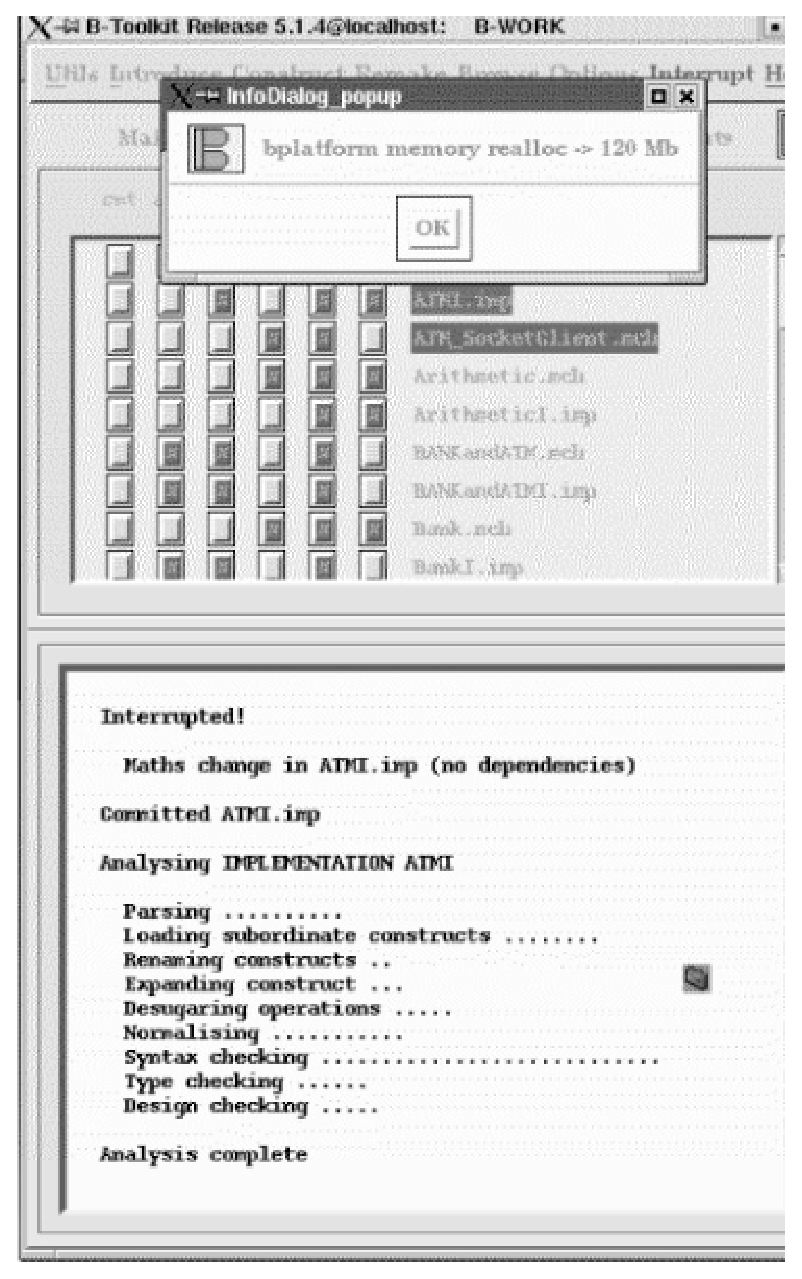
\epsfig{file=pic/memalloc120MB.eps}
	
An attempt to refine this system into an implementation should 
make the buffer model a starting point. This model should then
be re-specified using either the Protocol structure or
the sender-receiver structure.

This chapter has discussed a range of models and specifications which either allows
the specifier to state some global invariants about the system, 
eg the buffer specification and the protocol development,
and it has provided a model that allows for future refinements, ei the 
{\it SecureNetwork} development. But it has not been able to find a model that allows 
for both of these two functionalities at the same time. The {\it SecureNetwork}
specification does not give a global view of communication. Neither
the protocol development nor the buffer specification can easily be
refined into an {\it ATM} and a {\it Bank} machine.

\section{An attempt on Refining the Buffer specification}

Provided on the floppy disk, as mentioned in last section, is an attempt on 
specifying the ATM system with {\it ATM}, {\it Bank}, {\it BankSystem} and a 
{\it Globals} machine. This model avoids the problem of INCLUDES by letting {\it ATM} 
and {\it Bank} see {\it Globals}. {\it Globals} states the invariant that 
no money is lost over the network layer. Hence it must hold the set {\it totalBalance}. 
{\it ATM} and {\it Bank} attempt to update {\it totalBalance} but is not allowed
as variables of machines can only be modiefied by operations of that machine,
which is obvosly needed to generated consistency proof obligations.

\chapter{Using the B-Toolkit}

\section{Executing Implementations; Creating Interfaces}

An implementation may be executed by adding an interface of
the machine specification. For this project non-motif interfaces have been choosen. 
This option can be made by choosing Options - interface - non-motif. Then the 
interface is created by choosing Introduce - new - Interfaec of 
Implemented Machine and choosing the specification. The development must be converted 
to C code, compiled and linked. This is done in the generators environment. The code 
is executed in the translators environment.

The interface has this format: \newline
INTERFACE \quad    Arithmetic \newline
OPERATIONS \newline
\quad  exp\_op \newline
$<$ list of operations $>$ \newline
END

For the implementation of the ATM system it is nessesary to set
the option -DTEST\_FLAG under Options - Translateors\\Compilors menu,
and choose the C Compilor/Flags line.

\chapter{Conclusion}

\section{Topics Covered by this Project}

This project has covered three major topics.
\begin{itemize}
	\item Number theory and cryptology
	\item Formal proofs applied to the BToolkit
	\item The B-Method and in particular an investigation into models using
		machine composing constructs.
\end{itemize}
In that order.

\section{What to have in Mind when Writing a Specification}

Writing specifications is very different to programming. Writing specifications
require you to think carefully about what you are specifying. During this project
I have found that I repetedly keept changing specifications to better
model what I intend it to specify. When I program, I find myself often 
mindlessly hacking away at a problem because of some bug. 
When writing specifications you have to think "What do I want to say? 
Do these invariants express this in the best possible way?".
Very often there is no yes-no answer to this. I have used tools to help 
you obtain an answer though. This is the animator functionality in the BToolkit 
and most importantly the provers environment.

When writing specifications two things should be in mind
\begin{itemize}
	\item What functionality shall it present?
	\item What invariants need it preserve?
\end{itemize}

These two do not nessesarily conjoin. Maybe the invariant can
be expressed but not proven or the invaraint cannot be expressed at a level.
Finding the right place to state an invariant is well illustrated in
the airtraffic control system discussed in [1], where {\it ATCSystem}
expresses the invariant "all aircraft in a given airspace are 
controlled by the controller assigned to that airspace", expressed by \newline
$\forall(acft, as).(acft \in aircraft \wedge as \in airspaces \wedge
		acft \in occupied_by(as) \Rightarrow
			acft \in controls(assigned(as)) )$\newline
in {\it ATCSystem} because neither {\it Aircraft} nor {\it Controller}
has sufficient knowledge to express this.

\section{Why is B a Difficult Language to Learn?}

Firstly, anyone using B should have a firm knowledge of set theory and 
formal methods. Secondly, the the B syntax is not easily understood
coming from a classical programming background. The B syntax has many 
small oddities. Eg. "-0 is not element in $\nat$ and will give you a
parse error, but it surely is defined
as 0. The BToolkit also gives poor feedback on errors, eg. to show special 
rules of B is:
operation: \newline
\quad  status $\Leftarrow$ ATM\_create\_account = \newline
\indent	$creq := creq \leftarrow 1 $\newline
It parses and analysises fine

\quad  status $\Leftarrow$ ATM\_create\_account = \newline
\indent	$creq$ $:=$ $creq$ $\leftarrow$ $1$ \bparallel \newline
\indent	$status := TRUE$ \newline
does not. It should be modified to:\newline
\quad  status $\Leftarrow$ ATM\_create\_account = \newline
\indent	BEGIN
\indent\indent	$creq$ $:=$ $creq$ $\leftarrow$ $1$ \bparallel
\indent\indent	status := TRUE
\indent	END

\section{Final thoughts}

This project has shown refinement of algorithms into code, proof
of classical mathematics and logic in the BToolkit and that a development
can be formaly proven. In the ATM development different patterns
to express global invariants have been investigated.
With the aditional goal of still allowing for refinement.

From the ATM development I would not recommend the B-Method for specifying
and implementing transaction and concurrency systems. If we
look at the components of the ATM system, we have two distinct systems,
the ATM and the bank. They communicate, but in an implemention,
where would we be able constrain that no money is lost over the network layer?
There are other formalisems that have delved into this area, one is CSP.

I would say that the B-Method is suited for algorithm refinement, and
for applications which manage and manipulate large amounts of data. 
The effort it takes to develop applications in B should make you carefully
decide if the system is so safety-critical that it should use
formal methods to verify its correctness. In some industries, formal methods
is mandatory, like in the development of key-cards.

\chapter*{References}

The following papers have been consulted during the project:

\begin{itemize}

\item {[1]}\quad K. Lano, H. Haughton \quad
Specification in B An Introduction using the B Toolkit, Imperial College Press,1996.
ISBN: 1-86094-008-0

\item {[2]}\quad S. Schneider \quad
the b-method an introduction, Palgrave, 2001. ISBN: 0-333-79284-X

\item {[3]}\quad J-R Abrial \quad
the b-book, assigning programs to meanings, Cambridge University Press, 1996.
ISBN: 0-521-49619-5

\item {[4]}\quad E. Sekerinski, K. Sere \quad
program development by refinement case studies using the B method, Springer, 1999.
ISBN: 1852330538

\item {[5]}\quad E. Dijkstra \quad
A disipline of Programming, Prentice Hall 1976,
ISBN:

\item {[6]}\quad J. Seberry, J. Pieprzyk \quad
Cryptography an introdution to computer security, Prentice Hall, 1989.
ISBN: 0-7248-0274-6

\item {[7]}\quad T. H. Corman, C. E Leiserson, R. L Rivest \quad
Introduction to Algorithms, The MIT Press, 1999. 
ISBN: 0-262-53091-0

\item {[8]}\quad F. Zeyda \quad
Investigation of the B Method, Diploma arbeit, University of Teesside, 2002

\item {[9]}\quad S. Schneider \quad
Concurrent and Rea-time Systems the CSP approach, Wiley, 1999

\item {[10]}\quad B. Forouzan \quad
Date Communications and Networking, McGraw-Hill, 1998.
ISBN: 0-07-282294-5

\item {[11]}\quad Silberschatz, Galvin \quad
Operating System Concepts, Addison Wesley, 1997.
ISBN: 0-201-59113-8

\item {[12]}\quad S. Dunne \quad
A Theory of Generalised Substitutaions. In Springer, editor,
{\it ZB2002: Formal Specification and Develoment in Z and B}, Lecture
Notes in Computer Science 2272, 2002

\item {[13]}\quad B-Core(UK) \quad
B-Toolkit User's Manual. Technical report, 1997

\end{itemize}

\appendix
\chapter{Cipher Development}

%%%%%%%%%%%%%%%%%%%%%%%%%%%%%%%%%%%%%%%%%%  Arithmetic.mch.tex
%
\bsetindent
\begin{tabbing}
\bSetTabs
%
%%%%%%%%%%%%%%%%%%%%%%%%%%%%%%%%%%%%%%%%%%  MACHINE
%
\bbnl
{\bf MACHINE} \bhsp\+{\em Arithmetic\/} \-\label{Arithmetic}\index{Arithmetic}
%
%%%%%%%%%%%%%%%%%%%%%%%%%%%%%%%%%%%%%%%%%%  CONSTANTS
%
\bbnl
{\bf CONSTANTS} \+ \bbnl
{\em prime\/}\label{prime}\index{prime}  , {\em exp\/}\label{exp}\index{exp}  \-
%
%%%%%%%%%%%%%%%%%%%%%%%%%%%%%%%%%%%%%%%%%%  PROPERTIES
%
\bbnl
{\bf PROPERTIES} \+ \bbnl
{\em exp\/} $\in$  $\nat$  $\times$  $\nat$  $\pfun$  $\nat$  $\wedge$ \bnl
$\forall$ ( {\em aa\/} , {\em bb\/} ) . ( {\em aa\/} $\in$  $\nat$  $\wedge$
{\em bb\/} $\in$  $\nat\bsub{1}$  $\Rightarrow$
{\em exp\/} ( {\em aa\/} , {\em bb\/} )  $=$ {\em exp\/} ( {\em aa\/} , {\em bb\/} $-$ {\em 1\/} )  $\times$ {\em aa\/} $\wedge$ \bnl
{\em exp\/} ( {\em aa\/} , {\em 1\/} )  $=$ {\em aa\/} $\wedge$ \bnl
{\em exp\/} ( {\em bb\/} , {\em 0\/} )  $=$ {\em 1\/} $\wedge$ \bnl
{\em exp\/} ( {\em 0\/} , {\em bb\/} )  $=$ {\em 0\/} ) $\wedge$ \bnl
{\em prime\/} $\subseteq$  $\nat$  \-
%
%%%%%%%%%%%%%%%%%%%%%%%%%%%%%%%%%%%%%%%%%%  OPERATIONS
%
\bnl\bnl
{\bf OPERATIONS} \+ \bbnl

%
%%%%%%%%%%%%%%%%%%%%%%%%%%%%%%%%%%%%%%%%%%  OPERATION exp\_op
%
{\em rr\/} $\longleftarrow$  {\bf { exp\_op}} ( {\em aa\/} , {\em bb\/} ) \bhsp $\defs$ \+ \bnl
 \bOpnWord{PRE} \+\bnl
{\em aa\/} $\in$  $\nat$  $\wedge$ \bnl
{\em bb\/} $\in$  $\nat$  \-\bnl
\bOpnWord{THEN} \+\bnl
{\em rr\/} $:=$  {\em exp\/} ( {\em aa\/} , {\em bb\/} )  \-\bnl
\bOpnWord{END}  \-\- \bbnl

%
%%%%%%%%%%%%%%%%%%%%%%%%%%%%%%%%%%%%%%%%%%  END
%
\bbnl
{\bf END} 
\end{tabbing}
\bresetindent

%%%%%%%%%%%%%%%%%%%%%%%%%%%%%%%%%%%%%%%%%%  ArithmeticI.imp.tex
%
\bsetindent
\begin{tabbing}
\bSetTabs
%
%%%%%%%%%%%%%%%%%%%%%%%%%%%%%%%%%%%%%%%%%%  IMPLEMENTATION
%
\bbnl
{\bf IMPLEMENTATION} \bhsp\+{\em ArithmeticI\/} \-\label{ArithmeticI}\index{ArithmeticI}
%
%%%%%%%%%%%%%%%%%%%%%%%%%%%%%%%%%%%%%%%%%%  REFINES
%
\bbnl
{\bf REFINES} \+ \bbnl
{\em Arithmetic\/}\label{Arithmetic}\index{Arithmetic}  \-
%
%%%%%%%%%%%%%%%%%%%%%%%%%%%%%%%%%%%%%%%%%%  OPERATIONS
%
\bnl\bnl
{\bf OPERATIONS} \+ \bbnl

%
%%%%%%%%%%%%%%%%%%%%%%%%%%%%%%%%%%%%%%%%%%  OPERATION exp\_op
%
{\em rr\/} $\longleftarrow$  {\bf { exp\_op}} ( {\em aa\/} , {\em bb\/} ) \bhsp $\defs$ \+ \bnl
 \bOpnWord{IF} \+{\em aa\/} $\neq$ {\em 0\/} $\vee$
{\em bb\/} $\neq$ {\em 0\/} \- \bhsp \bOpnWord{THEN} \+\bnl
\bOpnWord{VAR} \+\bnl
{\em ii\/} , \bnl
{\em kk\/} \-\bnl
\bOpnWord{IN} \+\bnl
{\em ii\/} $:=$  {\em bb\/} \bStatementSemiColon \bnl
{\em kk\/} $:=$  {\em 1\/} \bStatementSemiColon \bnl
\bOpnWord{WHILE} \+\bnl
{\em ii\/} $\neq$ {\em 0\/} \-\bnl
\bOpnWord{DO} \+\bnl
{\em kk\/} $:=$  {\em kk\/} $\times$ {\em aa\/} \bStatementSemiColon \bnl
{\em ii\/} $:=$  {\em ii\/} $-$ {\em 1\/} \-\bnl
\bOpnWord{INVARIANT} \+\bnl
{\em ii\/} $\in$  $\nat$  $\wedge$ \bnl
{\em kk\/} $=$ {\em exp\/}\label{exp}\index{exp}  ( {\em aa\/} , {\em bb\/} $-$ {\em ii\/} )  \-\bnl
\bOpnWord{VARIANT} \+\bnl
{\em ii\/} \-\bnl
\bOpnWord{END}  \bStatementSemiColon \bnl
{\em rr\/} $:=$  {\em kk\/} \-\bnl
\bOpnWord{END}  \-\bnl
\bOpnWord{END}  \-
\end{tabbing}
\bresetindent
%
%%%%%%%%%%%%%%%%%%%%%%%%% Clause cross-references
%
\bxrefhead{Cross-references}
\bxrefline{{\em exp}}{{\em Arithmetic}}{{\sc constants}}{\bbpageref{exp}}
\vspace{-4.5ex}\bsetindent
\begin{tabbing}
\bSetTabs
\+\> \-
%
%%%%%%%%%%%%%%%%%%%%%%%%%%%%%%%%%%%%%%%%%%  END
%
\bbnl
{\bf END} 
\end{tabbing}
\bresetindent
%
%%%%%%%%%%%%%%%%%%%%%%%%% Construct cross-references for ArithmeticI
%
\bxrefhead{Cross-references for ArithmeticI}
\bxrefline{{\em Arithmetic}}{}{{\sc machine}}{\bbpageref{Arithmetic}}
\bxrefline{{\em exp}}{{\em Arithmetic}}{{\sc constants}}{\bbpageref{exp}}
\vskip 3.5ex

%%%%%%%%%%%%%%%%%%%%%%%%%%%%%%%%%%%%%%%%%%  Cipher.mch.tex
%
\bsetindent
\begin{tabbing}
\bSetTabs
%
%%%%%%%%%%%%%%%%%%%%%%%%%%%%%%%%%%%%%%%%%%  MACHINE
%
\bbnl
{\bf MACHINE} \bhsp\+{\em Cipher\/} ( {\em ee\/} , {\em dd\/} , {\em nn\/} )  \-\label{Cipher}\index{Cipher}
%
%%%%%%%%%%%%%%%%%%%%%%%%%%%%%%%%%%%%%%%%%%  CONSTRAINTS
%
\bbnl
{\bf CONSTRAINTS} \+ \bbnl
{\em ee\/} $\in$  $\nat$  $\wedge$ \bnl
{\em dd\/} $\in$  $\nat$  $\wedge$ \bnl
{\em nn\/} $\in$  $\nat\bsub{1}$  $\wedge$ \bnl
{\em ee\/} $\times$ {\em dd\/} \ {\sf mod}\  ( {\em nn\/} $-$ {\em 1\/} )  $=$ {\em 1\/} \-
%
%%%%%%%%%%%%%%%%%%%%%%%%%%%%%%%%%%%%%%%%%%  SEES
%
\bbnl
{\bf SEES} \+ \bbnl
{\em Arithmetic\/}\label{Arithmetic}\index{Arithmetic}  \-
%
%%%%%%%%%%%%%%%%%%%%%%%%%%%%%%%%%%%%%%%%%%  CONSTANTS
%
\bbnl
{\bf CONSTANTS} \+ \bbnl
{\em encrypt\/}\label{encrypt}\index{encrypt}  , {\em decrypt\/}\label{decrypt}\index{decrypt}  \-
%
%%%%%%%%%%%%%%%%%%%%%%%%%%%%%%%%%%%%%%%%%%  PROPERTIES
%
\bbnl
{\bf PROPERTIES} \+ \bbnl
{\em encrypt\/} $\in$  $\nat$  $\fun$  $\nat$  $\wedge$ \bnl
{\em decrypt\/} $\in$  $\nat$  $\fun$  $\nat$  $\wedge$ \bnl
$\forall$ {\em mm\/} . ( {\em mm\/} $\in$ {\em 0\/} $\upto$ {\em nn\/} $-$ {\em 1\/} $\Rightarrow$
{\em encrypt\/} ( {\em decrypt\/} ( {\em mm\/} )  )  $=$ {\em mm\/} ) $\wedge$ \bnl
$\forall$ {\em mm\/} . ( {\em mm\/} $\in$ {\em 0\/} $\upto$ {\em nn\/} $-$ {\em 1\/} $\Rightarrow$
{\em decrypt\/} ( {\em encrypt\/} ( {\em mm\/} )  )  $=$ {\em mm\/} ) \-
%
%%%%%%%%%%%%%%%%%%%%%%%%%%%%%%%%%%%%%%%%%%  OPERATIONS
%
\bnl\bnl
{\bf OPERATIONS} \+ \bbnl

%
%%%%%%%%%%%%%%%%%%%%%%%%%%%%%%%%%%%%%%%%%%  OPERATION encrypt\_op
%
{\em rr\/} $\longleftarrow$  {\bf { encrypt\_op}} ( {\em mm\/} ) \bhsp $\defs$ \+ \bnl
 \bOpnWord{PRE} \+\bnl
{\em mm\/} $\in$ {\em 0\/} $\upto$ {\em nn\/} $-$ {\em 1\/} \-\bnl
\bOpnWord{THEN} \+\bnl
{\em rr\/} $:=$  {\em encrypt\/} ( {\em mm\/} )  \-\bnl
\bOpnWord{END}  \- \bOperationSemiColon \bbnl
%
%%%%%%%%%%%%%%%%%%%%%%%%%%%%%%%%%%%%%%%%%%  OPERATION decrypt\_op
%
{\em rr\/} $\longleftarrow$  {\bf { decrypt\_op}} ( {\em mm\/} ) \bhsp $\defs$ \+ \bnl
 \bOpnWord{PRE} \+\bnl
{\em mm\/} $\in$ {\em 0\/} $\upto$ {\em nn\/} $-$ {\em 1\/} \-\bnl
\bOpnWord{THEN} \+\bnl
{\em rr\/} $:=$  {\em decrypt\/} ( {\em mm\/} )  \-\bnl
\bOpnWord{END}  \-\- \bbnl

%
%%%%%%%%%%%%%%%%%%%%%%%%%%%%%%%%%%%%%%%%%%  END
%
\bbnl
{\bf END} 
\end{tabbing}
\bresetindent
%
%%%%%%%%%%%%%%%%%%%%%%%%% Construct cross-references for Cipher
%
\bxrefhead{Cross-references for Cipher}
\bxrefline{{\em Arithmetic}}{}{{\sc machine}}{\bbpageref{Arithmetic}}
\vskip 3.5ex

%%%%%%%%%%%%%%%%%%%%%%%%%%%%%%%%%%%%%%%%%%  ExponentialCipherRef.ref.tex
%
\bsetindent
\begin{tabbing}
\bSetTabs
%
%%%%%%%%%%%%%%%%%%%%%%%%%%%%%%%%%%%%%%%%%%  REFINEMENT
%
\bbnl
{\bf REFINEMENT} \bhsp\+{\em ExponentialCipherRef\/} \-\label{ExponentialCipherRef}\index{ExponentialCipherRef}
%
%%%%%%%%%%%%%%%%%%%%%%%%%%%%%%%%%%%%%%%%%%  REFINES
%
\bbnl
{\bf REFINES} \+ \bbnl
{\em Cipher\/}\label{Cipher}\index{Cipher}  \-
%
%%%%%%%%%%%%%%%%%%%%%%%%%%%%%%%%%%%%%%%%%%  SEES
%
\bbnl
{\bf SEES} \+ \bbnl
{\em Arithmetic\/}\label{Arithmetic}\index{Arithmetic}  \-
%
%%%%%%%%%%%%%%%%%%%%%%%%%%%%%%%%%%%%%%%%%%  OPERATIONS
%
\bnl\bnl
{\bf OPERATIONS} \+ \bbnl

%
%%%%%%%%%%%%%%%%%%%%%%%%%%%%%%%%%%%%%%%%%%  OPERATION encrypt\_op
%
{\em rr\/} $\longleftarrow$  {\bf { encrypt\_op}} ( {\em mm\/} ) \bhsp $\defs$ \+ \bnl
{\em rr\/} $:=$  {\em exp\/}\label{exp}\index{exp}  ( {\em mm\/} , {\em ee\/} )  \ {\sf mod}\ {\em nn\/} \- \bOperationSemiColon 
\end{tabbing}
\bresetindent
%
%%%%%%%%%%%%%%%%%%%%%%%%% Clause cross-references
%
\bxrefhead{Cross-references}
\bxrefline{{\em exp}}{{\em Arithmetic}}{{\sc constants}}{\bbpageref{exp}}
\vspace{-4.5ex}\bsetindent
\begin{tabbing}
\bSetTabs
\+\>
%
%%%%%%%%%%%%%%%%%%%%%%%%%%%%%%%%%%%%%%%%%%  OPERATION decrypt\_op
%
{\em rr\/} $\longleftarrow$  {\bf { decrypt\_op}} ( {\em mm\/} ) \bhsp $\defs$ \+ \bnl
{\em rr\/} $:=$  {\em exp\/}\label{exp}\index{exp}  ( {\em mm\/} , {\em dd\/} )  \ {\sf mod}\ {\em nn\/} \-
\end{tabbing}
\bresetindent
%
%%%%%%%%%%%%%%%%%%%%%%%%% Clause cross-references
%
\bxrefhead{Cross-references}
\bxrefline{{\em exp}}{{\em Arithmetic}}{{\sc constants}}{\bbpageref{exp}}
\vspace{-4.5ex}\bsetindent
\begin{tabbing}
\bSetTabs
\+\> \-
%
%%%%%%%%%%%%%%%%%%%%%%%%%%%%%%%%%%%%%%%%%%  END
%
\bbnl
{\bf END} 
\end{tabbing}
\bresetindent
%
%%%%%%%%%%%%%%%%%%%%%%%%% Construct cross-references for ExponentialCipherRef
%
\bxrefhead{Cross-references for ExponentialCipherRef}
\bxrefline{{\em Arithmetic}}{}{{\sc machine}}{\bbpageref{Arithmetic}}
\bxrefline{{\em Cipher}}{}{{\sc machine}}{\bbpageref{Cipher}}
\bxrefline{{\em exp}}{{\em Arithmetic}}{{\sc constants}}{\bbpageref{exp}}
\vskip 3.5ex

%%%%%%%%%%%%%%%%%%%%%%%%%%%%%%%%%%%%%%%%%%  ExponentialCipherI.imp.tex
%
\bsetindent
\begin{tabbing}
\bSetTabs
%
%%%%%%%%%%%%%%%%%%%%%%%%%%%%%%%%%%%%%%%%%%  IMPLEMENTATION
%
\bbnl
{\bf IMPLEMENTATION} \bhsp\+{\em ExponentialCipherI\/} \-\label{ExponentialCipherI}\index{ExponentialCipherI}
%
%%%%%%%%%%%%%%%%%%%%%%%%%%%%%%%%%%%%%%%%%%  REFINES
%
\bbnl
{\bf REFINES} \+ \bbnl
{\em ExponentialCipherRef\/}\label{ExponentialCipherRef}\index{ExponentialCipherRef}  \-
%
%%%%%%%%%%%%%%%%%%%%%%%%%%%%%%%%%%%%%%%%%%  IMPORTS
%
\bbnl
{\bf IMPORTS} \+ \bbnl
{\em Arithmetic\/}\label{Arithmetic}\index{Arithmetic}  \-
%
%%%%%%%%%%%%%%%%%%%%%%%%%%%%%%%%%%%%%%%%%%  OPERATIONS
%
\bnl\bnl
{\bf OPERATIONS} \+ \bbnl

%
%%%%%%%%%%%%%%%%%%%%%%%%%%%%%%%%%%%%%%%%%%  OPERATION encrypt\_op
%
{\em rr\/} $\longleftarrow$  {\bf { encrypt\_op}} ( {\em mm\/} ) \bhsp $\defs$ \+ \bnl
 \bOpnWord{VAR} \+{\em tmp\/} \- \bhsp \bOpnWord{IN} \+\bnl
{\em tmp\/} $\longleftarrow$ {\em exp\_op\/}\label{exp_op}\index{exp_op}  ( {\em mm\/} , {\em ee\/} )  \bStatementSemiColon \bnl
{\em rr\/} $:=$  {\em tmp\/} \ {\sf mod}\ {\em nn\/} \-\bnl
\bOpnWord{END}  \- \bOperationSemiColon 
\end{tabbing}
\bresetindent
%
%%%%%%%%%%%%%%%%%%%%%%%%% Clause cross-references
%
\bxrefhead{Cross-references}
\bxrefline{{\em exp\_op}}{{\em Arithmetic}}{{\sc operations}}{\bbpageref{exp_op}}
\vspace{-4.5ex}\bsetindent
\begin{tabbing}
\bSetTabs
\+\>
%
%%%%%%%%%%%%%%%%%%%%%%%%%%%%%%%%%%%%%%%%%%  OPERATION decrypt\_op
%
{\em rr\/} $\longleftarrow$  {\bf { decrypt\_op}} ( {\em mm\/} ) \bhsp $\defs$ \+ \bnl
 \bOpnWord{VAR} \+{\em tmp\/} \- \bhsp \bOpnWord{IN} \+\bnl
{\em tmp\/} $\longleftarrow$ {\em exp\_op\/}\label{exp_op}\index{exp_op}  ( {\em mm\/} , {\em dd\/} )  \bStatementSemiColon \bnl
{\em rr\/} $:=$  {\em tmp\/} \ {\sf mod}\ {\em nn\/} \-\bnl
\bOpnWord{END}  \-
\end{tabbing}
\bresetindent
%
%%%%%%%%%%%%%%%%%%%%%%%%% Clause cross-references
%
\bxrefhead{Cross-references}
\bxrefline{{\em exp\_op}}{{\em Arithmetic}}{{\sc operations}}{\bbpageref{exp_op}}
\vspace{-4.5ex}\bsetindent
\begin{tabbing}
\bSetTabs
\+\> \-
%
%%%%%%%%%%%%%%%%%%%%%%%%%%%%%%%%%%%%%%%%%%  END
%
\bbnl
{\bf END} 
\end{tabbing}
\bresetindent
%
%%%%%%%%%%%%%%%%%%%%%%%%% Construct cross-references for ExponentialCipherI
%
\bxrefhead{Cross-references for ExponentialCipherI}
\bxrefline{{\em Arithmetic}}{}{{\sc machine}}{\bbpageref{Arithmetic}}
\bxrefline{{\em ExponentialCipherRef}}{}{{\sc refinement}}{\bbpageref{ExponentialCipherRef}}
\bxrefline{{\em exp\_op}}{{\em Arithmetic}}{{\sc operations}}{\bbpageref{exp_op}}
\vskip 3.5ex

\section{Proof Prints}
%%%%%%%%%%%%%%%
%%%%%%%%%%%%%%%%%%%%  Arithmetic.mch.prf.0
%%%%%%%%%%%%%%%
\begin{center}
{\large {\bf Proofs (Level 0) for Arithmetic.mch}}
\end{center}
%%%%%%%%%%%%%%%
%%%%%%%%%%%%%%%%%%%%  Context.1
%%%%%%%%%%%%%%%
\rule{\textwidth}{.1ex} \bnl
\underline{{\em Context.1\/}} \bbnl
\bproofline{1}{{\em cst\/} ( {\em Arithmetic\/} ) }{{\sf HYP}}
\bproofline{2}{ \bhsp $\exists$ {\em prime\/} . ( {\em prime\/} $\subseteq$  $\nat$  )}{{\sf BToolUsersTheory.1}}
\bproofline{3}{{\em QED\/}}{{\sf DED}}
\rule{\textwidth}{.1ex} \bnl
{\bf Laws (Level 0) for Arithmetic.mch } \bbnl
\underline{{\sf BToolUsersTheory.1}} \bbnl
  $\exists$  $p$  . (  $p$  $\subseteq$  $\nat$  )

%%%%%%%%%%%%%%%
%%%%%%%%%%%%%%%%%%%%  ArithmeticI.imp.prf.1
%%%%%%%%%%%%%%%
\begin{center}
{\large {\bf Proofs (Level 1) for ArithmeticI.imp}}
\end{center}
%%%%%%%%%%%%%%%
%%%%%%%%%%%%%%%%%%%%  exp\_op.2
%%%%%%%%%%%%%%%
\rule{\textwidth}{.1ex} \bnl
\underline{{\em exp\_op.2\/}} \bbnl
\bproofline{1}{{\em cst\/} ( {\em ArithmeticI\/} $\bsub{1}$ ) }{{\sf HYP}}
\bproofline{2}{{\em ctx\/} ( {\em ArithmeticI\/} $\bsub{1}$ ) }{{\sf HYP}}
\bproofline{3}{{\em inv\/} ( {\em ArithmeticI\/} $\bsub{1}$ ) }{{\sf HYP}}
\bproofline{4}{{\em asn\/} ( {\em ArithmeticI\/} $\bsub{1}$ ) }{{\sf HYP}}
\bproofline{5}{{\em pre\/} ( {\em exp\_op\/} ) }{{\sf HYP}}
\bproofline{6}{ \bhsp{\em aa\/} $\in$  $\nat$ }{{\sf 5}, {\sf HypExp.1}}
\bproofline{7}{ \bhsp $\neg$  ( {\em aa\/} $=$ {\em 0\/} ) }{{\sf HYP}}
\bproofline{8}{ \bhsp{\em ii\/} $\in$  $\nat$ }{{\sf HYP}}
\bproofline{9}{ \bhsp{\em kk\/} $=$ {\em exp\/} ( {\em aa\/} , {\em bb\/} $-$ {\em ii\/} ) }{{\sf HYP}}
\bproofline{10}{ \bhsp $\neg$  ( {\em ii\/} $=$ {\em 0\/} ) }{{\sf HYP}}
\bproofline{11}{ \bhsp{\em exp\/} ( {\em aa\/} , {\em bb\/} $-$ {\em ii\/} $+$ {\em 1\/} )  $=$ {\em exp\/} ( {\em aa\/} , {\em bb\/} $-$ {\em ii\/} $+$ {\em 1\/} ) }{{\sf EQL}}
\bproofline{12}{ \bhsp{\em exp\/} ( {\em aa\/} , {\em bb\/} $-$ {\em ii\/} $+$ {\em 1\/} )  $=$ {\em exp\/} ( {\em aa\/} , {\em bb\/} $-$  ( {\em ii\/} $-$ {\em 1\/} )  ) }{{\sf 11}, {\sf Law.1}}
\bproofline{13}{ \bhsp{\em exp\/} ( {\em aa\/} , {\em bb\/} $-$ {\em ii\/} )  $\times$ {\em aa\/} $=$ {\em exp\/} ( {\em aa\/} , {\em bb\/} $-$  ( {\em ii\/} $-$ {\em 1\/} )  ) }{{\sf 6}, {\sf 12}, {\sf BToolUsersTheory.1}}
\bproofline{14}{ \bhsp{\em kk\/} $\times$ {\em aa\/} $=$ {\em exp\/} ( {\em aa\/} , {\em bb\/} $-$  ( {\em ii\/} $-$ {\em 1\/} )  ) }{{\sf 13}, {\sf 9}}
\bproofline{15}{{\em QED\/}}{{\sf DED}}
%%%%%%%%%%%%%%%
%%%%%%%%%%%%%%%%%%%%  exp\_op.5
%%%%%%%%%%%%%%%
\rule{\textwidth}{.1ex} \bnl
\underline{{\em exp\_op.5\/}} \bbnl
\bproofline{1}{{\em cst\/} ( {\em ArithmeticI\/} $\bsub{1}$ ) }{{\sf HYP}}
\bproofline{2}{{\em ctx\/} ( {\em ArithmeticI\/} $\bsub{1}$ ) }{{\sf HYP}}
\bproofline{3}{{\em inv\/} ( {\em ArithmeticI\/} $\bsub{1}$ ) }{{\sf HYP}}
\bproofline{4}{{\em asn\/} ( {\em ArithmeticI\/} $\bsub{1}$ ) }{{\sf HYP}}
\bproofline{5}{{\em pre\/} ( {\em exp\_op\/} ) }{{\sf HYP}}
\bproofline{6}{ \bhsp{\em bb\/} $\in$  $\nat$ }{{\sf 5}, {\sf HypExp.2}}
\bproofline{7}{ \bhsp{\em aa\/} $\in$  $\nat$ }{{\sf 5}, {\sf HypExp.1}}
\bproofline{8}{ \bhsp $\neg$  ( {\em aa\/} $=$ {\em 0\/} ) }{{\sf HYP}}
\bproofline{9}{ \bhsp{\em aa\/} $\in$  $\nat\bsub{1}$ }{{\sf 8}, {\sf 7}, {\sf Law.2}}
\bproofline{10}{ \bhsp{\em exp\/} ( {\em aa\/} , {\em 0\/} )  $=$ {\em exp\/} ( {\em aa\/} , {\em 0\/} ) }{{\sf EQL}}
\bproofline{11}{ \bhsp{\em exp\/} ( {\em aa\/} , {\em 0\/} )  $=$ {\em exp\/} ( {\em aa\/} , {\em bb\/} $-$ {\em bb\/} ) }{{\sf 6}, {\sf 10}, {\sf Law.3}}
\bproofline{12}{ \bhsp{\em 1\/} $=$ {\em exp\/} ( {\em aa\/} , {\em bb\/} $-$ {\em bb\/} ) }{{\sf 9}, {\sf 11}, {\sf BToolUsersTheory.2}}
\bproofline{13}{{\em QED\/}}{{\sf DED}}
%%%%%%%%%%%%%%%
%%%%%%%%%%%%%%%%%%%%  exp\_op.7
%%%%%%%%%%%%%%%
\rule{\textwidth}{.1ex} \bnl
\underline{{\em exp\_op.7\/}} \bbnl
\bproofline{1}{{\em cst\/} ( {\em ArithmeticI\/} $\bsub{1}$ ) }{{\sf HYP}}
\bproofline{2}{{\em ctx\/} ( {\em ArithmeticI\/} $\bsub{1}$ ) }{{\sf HYP}}
\bproofline{3}{{\em inv\/} ( {\em ArithmeticI\/} $\bsub{1}$ ) }{{\sf HYP}}
\bproofline{4}{{\em asn\/} ( {\em ArithmeticI\/} $\bsub{1}$ ) }{{\sf HYP}}
\bproofline{5}{{\em pre\/} ( {\em exp\_op\/} ) }{{\sf HYP}}
\bproofline{6}{ \bhsp{\em aa\/} $\in$  $\nat$ }{{\sf 5}, {\sf HypExp.1}}
\bproofline{7}{ \bhsp $\neg$  ( {\em bb\/} $=$ {\em 0\/} ) }{{\sf HYP}}
\bproofline{8}{ \bhsp{\em ii\/} $\in$  $\nat$ }{{\sf HYP}}
\bproofline{9}{ \bhsp{\em kk\/} $=$ {\em exp\/} ( {\em aa\/} , {\em bb\/} $-$ {\em ii\/} ) }{{\sf HYP}}
\bproofline{10}{ \bhsp $\neg$  ( {\em ii\/} $=$ {\em 0\/} ) }{{\sf HYP}}
\bproofline{11}{ \bhsp{\em exp\/} ( {\em aa\/} , {\em bb\/} $-$ {\em ii\/} $+$ {\em 1\/} )  $=$ {\em exp\/} ( {\em aa\/} , {\em bb\/} $-$ {\em ii\/} $+$ {\em 1\/} ) }{{\sf EQL}}
\bproofline{12}{ \bhsp{\em exp\/} ( {\em aa\/} , {\em bb\/} $-$ {\em ii\/} $+$ {\em 1\/} )  $=$ {\em exp\/} ( {\em aa\/} , {\em bb\/} $-$  ( {\em ii\/} $-$ {\em 1\/} )  ) }{{\sf 11}, {\sf Law.1}}
\bproofline{13}{ \bhsp{\em exp\/} ( {\em aa\/} , {\em bb\/} $-$ {\em ii\/} )  $\times$ {\em aa\/} $=$ {\em exp\/} ( {\em aa\/} , {\em bb\/} $-$  ( {\em ii\/} $-$ {\em 1\/} )  ) }{{\sf 6}, {\sf 12}, {\sf BToolUsersTheory.1}}
\bproofline{14}{ \bhsp{\em kk\/} $\times$ {\em aa\/} $=$ {\em exp\/} ( {\em aa\/} , {\em bb\/} $-$  ( {\em ii\/} $-$ {\em 1\/} )  ) }{{\sf 13}, {\sf 9}}
\bproofline{15}{{\em QED\/}}{{\sf DED}}
\rule{\textwidth}{.1ex} \bnl
{\bf Laws (Level 1) for ArithmeticI.imp } \bbnl
\underline{{\sf HypExp.1}} \bbnl
 {\em pre\/} ( {\em exp\_op\/} ) \bnl
$\Rightarrow$ \bnl
 {\em aa\/} $\in$  $\nat$ \bbnl
\underline{{\sf HypExp.2}} \bbnl
 {\em pre\/} ( {\em exp\_op\/} ) \bnl
$\Rightarrow$ \bnl
 {\em bb\/} $\in$  $\nat$ \bbnl
\underline{{\sf BToolUsersTheory.1}} \bbnl
 {\em aa\/} $\in$  $\nat$ \bnl
$\Rightarrow$ \bnl
 {\em exp\/} ( {\em aa\/} ,  $b$  )  $\times$ {\em aa\/} $\;\;\defs\;\;$ {\em exp\/} ( {\em aa\/} ,  $b$  $+$ {\em 1\/} ) \bbnl
\underline{{\sf BToolUsersTheory.2}} \bbnl
 {\em aa\/} $\in$  $\nat\bsub{1}$ \bnl
$\Rightarrow$ \bnl
 {\em 1\/} $\;\;\defs\;\;$ {\em exp\/} ( {\em aa\/} , {\em 0\/} ) \bbnl
\underline{{\sf Law.1} ({\sf RewriteAlgebra2X.8})} \bbnl
  $c$  $\in$ {\em 0\/} $\upto$ {\em 2147483647\/}\bnl
$\Rightarrow$ \bnl
  $a$  $-$  (  $b$  $-$  $c$  )  $\;\;\defs\;\;$  $a$  $-$  $b$  $+$  $c$ \bbnl
\underline{{\sf Law.2} ({\sf FwdInNat1X.17})} \bbnl
  $\neg$  (  $n$  $=$ {\em 0\/} )  $\wedge$
$n$  $\in$  $\nat$ \bnl
$\Rightarrow$ \bnl
  $n$  $\in$  $\nat\bsub{1}$ \bbnl
\underline{{\sf Law.3} ({\sf RewriteNat0X.2})} \bbnl
  $a$  $\in$  $\nat$ \bnl
$\Rightarrow$ \bnl
  $a$  $-$  $a$  $\;\;\defs\;\;$ {\em 0\/}

%%%%%%%%%%%%%%%
%%%%%%%%%%%%%%%%%%%%  Cipher.mch.prf.0
%%%%%%%%%%%%%%%
\begin{center}
{\large {\bf Proofs (Level 0) for Cipher.mch}}
\end{center}
%%%%%%%%%%%%%%%
%%%%%%%%%%%%%%%%%%%%  Constraints.1
%%%%%%%%%%%%%%%
\rule{\textwidth}{.1ex} \bnl
\underline{{\em Constraints.1\/}} \bbnl
\bproofline{1}{{\em 1\/} $=$ {\em 1\/}}{{\sf EQL}}
\bproofline{2}{{\em 1\/} $-$ {\em 0\/} $=$ {\em 1\/}}{{\sf 1}, {\sf ARI}}
\bproofline{3}{{\em 1\/} $-$ {\em 0\/} $\times$ {\em 2\/} $=$ {\em 1\/}}{{\sf 2}, {\sf ARI}}
\bproofline{4}{{\em 1\/} $-$ {\em 1\/}  / {\em 2\/} $\times$ {\em 2\/} $=$ {\em 1\/}}{{\sf 3}, {\sf ARI}}
\bproofline{5}{{\em 1\/} \ {\sf mod}\ {\em 2\/} $=$ {\em 1\/}}{{\sf 4}, {\sf Law.1}}
\bproofline{6}{{\em 1\/} $\times$ {\em 1\/} \ {\sf mod}\ {\em 2\/} $=$ {\em 1\/}}{{\sf 5}, {\sf ARI}}
\bproofline{7}{ $\char91$ {\em ee\/} $:=$ {\em 1\/} $\char93$  ( {\em ee\/} $\times$ {\em 1\/} \ {\sf mod}\ {\em 2\/} $=$ {\em 1\/} ) }{{\sf 6}, {\sf SUB}}
\bproofline{8}{ $\exists$ {\em ee\/} . ( {\em ee\/} $\in$  $\nat$  $\wedge$
{\em ee\/} $\times$ {\em 1\/} \ {\sf mod}\ {\em 2\/} $=$ {\em 1\/} )}{{\sf 7}, {\sf Law.2}}
\bproofline{9}{ $\exists$ {\em ee\/} .  $\char91$ {\em dd\/} $:=$ {\em 1\/} $\char93$  ( {\em ee\/} $\in$  $\nat$  $\wedge$
{\em ee\/} $\times$ {\em dd\/} \ {\sf mod}\ {\em 2\/} $=$ {\em 1\/} ) }{{\sf 8}, {\sf SUB}}
\bproofline{10}{ $\exists$ {\em dd\/} , {\em ee\/} . ( \bnl
& \bhsp  \bhsp {\em dd\/} $\in$  $\nat$  $\wedge$ \bnl
& \bhsp  \bhsp {\em ee\/} $\in$  $\nat$  $\wedge$ \bnl
& \bhsp  \bhsp {\em ee\/} $\times$ {\em dd\/} \ {\sf mod}\ {\em 2\/} $=$ {\em 1\/} ) }{{\sf 9}, {\sf Law.3}}
\bproofline{11}{ $\exists$ {\em dd\/} , {\em ee\/} . ( \bnl
& \bhsp  \bhsp {\em dd\/} $\in$  $\nat$  $\wedge$ \bnl
& \bhsp  \bhsp {\em ee\/} $\in$  $\nat$  $\wedge$ \bnl
& \bhsp  \bhsp {\em ee\/} $\times$ {\em dd\/} \ {\sf mod}\  ( {\em 3\/} $-$ {\em 1\/} )  $=$ {\em 1\/} ) }{{\sf 10}, {\sf ARI}}
\bproofline{12}{ $\exists$ {\em dd\/} , {\em ee\/} . ( \bnl
& \bhsp  $\char91$ {\em nn\/} $:=$  {\em 3\/} $\char93$  ( \bnl
& \bhsp  \bhsp {\em dd\/} $\in$  $\nat$  $\wedge$ \bnl
& \bhsp  \bhsp {\em ee\/} $\in$  $\nat$  $\wedge$ \bnl
& \bhsp  \bhsp {\em ee\/} $\times$ {\em dd\/} \ {\sf mod}\  ( {\em nn\/} $-$ {\em 1\/} )  $=$ {\em 1\/} ) }{{\sf 11}, {\sf SUB}}
\bproofline{13}{ $\exists$ {\em dd\/} , {\em nn\/} , {\em ee\/} . ( \bnl
& \bhsp  \bhsp {\em dd\/} $\in$  $\nat$  $\wedge$ \bnl
& \bhsp  \bhsp {\em ee\/} $\in$  $\nat$  $\wedge$ \bnl
& \bhsp  \bhsp {\em nn\/} $\in$  $\nat\bsub{1}$  $\wedge$ \bnl
& \bhsp  \bhsp {\em ee\/} $\times$ {\em dd\/} \ {\sf mod}\  ( {\em nn\/} $-$ {\em 1\/} )  $=$ {\em 1\/} ) }{{\sf 12}, {\sf BToolUsersTheory.1}}
\rule{\textwidth}{.1ex} \bnl
{\bf Laws (Level 0) for Cipher.mch } \bbnl
\underline{{\sf BToolUsersTheory.1}} \bbnl
  {\sf bsearch}$\;$(  (  $a$  $\in$  $\nat\bsub{1}$  )  ,  $b$  ,  $c$  )  $\wedge$
{\sf bsearch}$\;$(  $a$  ,  $A$  ,  $B$  )  $\wedge$
$\exists$  $B$  .  $\char91$  $a$  $:=$ {\em 3\/} $\char93$  $c$ \bnl
$\Rightarrow$ \bnl
  $\exists$  $A$  .  $b$ \bbnl
\underline{{\sf Law.1} ({\sf RewritePredicate0X.1})} \bbnl
  $a$  $\in$ {\em 0\/} $\upto$ {\em 2147483647\/} $\wedge$
$b$  $\in$ {\em 0\/} $\upto$ {\em 2147483647\/} $\wedge$
$b$  $>$ {\em 0\/}\bnl
$\Rightarrow$ \bnl
  $a$  \ {\sf mod}\  $b$  $\;\;\defs\;\;$  $a$  $-$  $a$   /  $b$  $\times$  $b$ \bbnl
\underline{{\sf Law.2} ({\sf Exist1X.15})} \bbnl
  {\sf bsearch}$\;$(  (  $a$  $\in$  $\nat$  )  ,  $b$  ,  $c$  )  $\wedge$
$\char91$  $a$  $:=$ {\em 1\/} $\char93$  $c$ \bnl
$\Rightarrow$ \bnl
  $\exists$  $a$  .  $b$ \bbnl
\underline{{\sf Law.3} ({\sf Exist1X.16})} \bbnl
  {\sf bsearch}$\;$(  (  $a$  $\in$  $\nat$  )  ,  $b$  ,  $c$  )  $\wedge$
{\sf bsearch}$\;$(  $a$  ,  $A$  ,  $B$  )  $\wedge$
$\exists$  $B$  .  $\char91$  $a$  $:=$ {\em 1\/} $\char93$  $c$ \bnl
$\Rightarrow$ \bnl
  $\exists$  $A$  .  $b$

%%%%%%%%%%%%%%%
%%%%%%%%%%%%%%%%%%%%  ExponentialCipherRef.ref.prf.0
%%%%%%%%%%%%%%%
\begin{center}
{\large {\bf Proofs (Level 0) for ExponentialCipherRef.ref}}
\end{center}
%%%%%%%%%%%%%%%
%%%%%%%%%%%%%%%%%%%%  Context.1
%%%%%%%%%%%%%%%
\rule{\textwidth}{.1ex} \bnl
\underline{{\em Context.1\/}} \bbnl
\bproofline{1}{{\em cst\/} ( {\em ExponentialCipherRef\/} $\bsub{1}$ ) }{{\sf HYP}}
\bproofline{2}{ \bhsp{\em nn\/} $\in$  $\nat\bsub{1}$ }{{\sf 1}, {\sf HypExp.9}}
\bproofline{3}{ \bhsp{\em ee\/} $\in$  $\nat$ }{{\sf 1}, {\sf HypExp.8}}
\bproofline{4}{ \bhsp{\em dd\/} $\in$  $\nat$ }{{\sf 1}, {\sf HypExp.7}}
\bproofline{5}{ \bhsp{\em ee\/} $\times$ {\em dd\/} \ {\sf mod}\  ( {\em nn\/} $-$ {\em 1\/} )  $=$ {\em 1\/}}{{\sf 1}, {\sf HypExp.6}}
\bproofline{6}{ \bhsp{\em nn\/} $\in$  $\nat$ }{{\sf 2}, {\sf Law.1}}
\bproofline{7}{ \bhsp{\em ctx\/} ( {\em Arithmetic\/} ) }{{\sf HYP}}
\bproofline{8}{ \bhsp $k$  $\in$  $\nat\bsub{1}$ }{{\sf BToolUsersTheory.6}}
\bproofline{9}{ \bhsp $k$  $\in$  $\nat$ }{{\sf 8}, {\sf BToolUsersTheory.8}}
\bproofline{10}{ \bhsp{\em 1\/} $\in$  $\nat$ }{{\sf Law.2}}
\bproofline{11}{ \bhsp{\em 1\/} $\leq$ {\em nn\/}}{{\sf 2}, {\sf Law.3}}
\bproofline{12}{ \bhsp{\em nn\/} $-$ {\em 1\/} $\in$  $\nat$ }{{\sf 6}, {\sf 10}, {\sf 11}, {\sf Law.4}}
\bproofline{13}{ \bhsp $k$  $\times$  ( {\em nn\/} $-$ {\em 1\/} )  $\in$  $\nat$ }{{\sf 9}, {\sf 12}, {\sf Law.5}}
\bproofline{14}{ \bhsp{\em 0\/} $<$ {\em 1\/}}{{\sf ARI}}
\bproofline{15}{ \bhsp{\em 1\/} $\in$  $\nat\bsub{1}$ }{{\sf 10}, {\sf 14}, {\sf Law.6}}
\bproofline{16}{ \bhsp $\exists$ {\em encrypt\/} , {\em decrypt\/} . ( \bnl
& \bhsp  \bhsp {\em encrypt\/} $\in$  $\nat$  $\fun$  $\nat$  $\wedge$ \bnl
& \bhsp  \bhsp {\em decrypt\/} $\in$  $\nat$  $\fun$  $\nat$  $\wedge$ \bnl
& \bhsp  \bhsp  $\forall$ {\em mm\/} . ( {\em mm\/} $\in$ {\em 0\/} $\upto$ {\em nn\/} $-$ {\em 1\/} $\Rightarrow$
{\em decrypt\/} ( {\em encrypt\/} ( {\em mm\/} )  )  $=$ {\em mm\/} ) ) }{{\sf BToolUsersTheory.18}}
\bproofline{17}{ \bhsp $\exists$ {\em encrypt\/} , {\em decrypt\/} . ( \bnl
& \bhsp  \bhsp {\em encrypt\/} $\in$  $\nat$  $\fun$  $\nat$  $\wedge$ \bnl
& \bhsp  \bhsp {\em decrypt\/} $\in$  $\nat$  $\fun$  $\nat$  $\wedge$ \bnl
& \bhsp  \bhsp {\em true\/} $\wedge$ \bnl
& \bhsp  \bhsp  $\forall$ {\em mm\/} . ( {\em mm\/} $\in$ {\em 0\/} $\upto$ {\em nn\/} $-$ {\em 1\/} $\Rightarrow$
{\em decrypt\/} ( {\em encrypt\/} ( {\em mm\/} )  )  $=$ {\em mm\/} ) ) }{{\sf 16}, {\sf Law.7}}
\bproofline{18}{ \bhsp $\exists$ {\em encrypt\/} , {\em decrypt\/} . ( \bnl
& \bhsp  \bhsp {\em encrypt\/} $\in$  $\nat$  $\fun$  $\nat$  $\wedge$ \bnl
& \bhsp  \bhsp {\em decrypt\/} $\in$  $\nat$  $\fun$  $\nat$  $\wedge$ \bnl
& \bhsp  \bhsp  $\forall$ {\em mm\/} . {\em true\/} $\wedge$ \bnl
& \bhsp  \bhsp  $\forall$ {\em mm\/} . ( {\em mm\/} $\in$ {\em 0\/} $\upto$ {\em nn\/} $-$ {\em 1\/} $\Rightarrow$
{\em decrypt\/} ( {\em encrypt\/} ( {\em mm\/} )  )  $=$ {\em mm\/} ) ) }{{\sf 17}, {\sf Law.8}}
\bproofline{19}{ \bhsp $\exists$ {\em encrypt\/} , {\em decrypt\/} . ( \bnl
& \bhsp  \bhsp {\em encrypt\/} $\in$  $\nat$  $\fun$  $\nat$  $\wedge$ \bnl
& \bhsp  \bhsp {\em decrypt\/} $\in$  $\nat$  $\fun$  $\nat$  $\wedge$ \bnl
& \bhsp  \bhsp  $\forall$ {\em mm\/} . ( {\em mm\/} $\in$ {\em 0\/} $\upto$ {\em nn\/} $-$ {\em 1\/} $\Rightarrow$
{\em true\/} ) $\wedge$ \bnl
& \bhsp  \bhsp  $\forall$ {\em mm\/} . ( {\em mm\/} $\in$ {\em 0\/} $\upto$ {\em nn\/} $-$ {\em 1\/} $\Rightarrow$
{\em decrypt\/} ( {\em encrypt\/} ( {\em mm\/} )  )  $=$ {\em mm\/} ) ) }{{\sf 18}, {\sf Law.9}}
\bproofline{20}{ \bhsp $\exists$ {\em encrypt\/} , {\em decrypt\/} . ( \bnl
& \bhsp  \bhsp {\em encrypt\/} $\in$  $\nat$  $\fun$  $\nat$  $\wedge$ \bnl
& \bhsp  \bhsp {\em decrypt\/} $\in$  $\nat$  $\fun$  $\nat$  $\wedge$ \bnl
& \bhsp  \bhsp  $\forall$ {\em mm\/} . ( {\em mm\/} $\in$ {\em 0\/} $\upto$ {\em nn\/} $-$ {\em 1\/} $\Rightarrow$
{\em mm\/} $=$ {\em mm\/} ) $\wedge$ \bnl
& \bhsp  \bhsp  $\forall$ {\em mm\/} . ( {\em mm\/} $\in$ {\em 0\/} $\upto$ {\em nn\/} $-$ {\em 1\/} $\Rightarrow$
{\em decrypt\/} ( {\em encrypt\/} ( {\em mm\/} )  )  $=$ {\em mm\/} ) ) }{{\sf 19}, {\sf Law.10}}
\bproofline{21}{ \bhsp $\exists$ {\em encrypt\/} , {\em decrypt\/} . ( \bnl
& \bhsp  \bhsp {\em encrypt\/} $\in$  $\nat$  $\fun$  $\nat$  $\wedge$ \bnl
& \bhsp  \bhsp {\em decrypt\/} $\in$  $\nat$  $\fun$  $\nat$  $\wedge$ \bnl
& \bhsp  \bhsp  $\forall$ {\em mm\/} . ( {\em mm\/} $\in$ {\em 0\/} $\upto$ {\em nn\/} $-$ {\em 1\/} $\Rightarrow$
{\em mm\/} \ {\sf mod}\ {\em nn\/} $=$ {\em mm\/} ) $\wedge$ \bnl
& \bhsp  \bhsp  $\forall$ {\em mm\/} . ( {\em mm\/} $\in$ {\em 0\/} $\upto$ {\em nn\/} $-$ {\em 1\/} $\Rightarrow$
{\em decrypt\/} ( {\em encrypt\/} ( {\em mm\/} )  )  $=$ {\em mm\/} ) ) }{{\sf 2}, {\sf 20}, {\sf BToolUsersTheory.17}}
\bproofline{22}{ \bhsp $\exists$ {\em encrypt\/} , {\em decrypt\/} . ( \bnl
& \bhsp  \bhsp {\em encrypt\/} $\in$  $\nat$  $\fun$  $\nat$  $\wedge$ \bnl
& \bhsp  \bhsp {\em decrypt\/} $\in$  $\nat$  $\fun$  $\nat$  $\wedge$ \bnl
& \bhsp  \bhsp  $\forall$ {\em mm\/} . ( {\em mm\/} $\in$ {\em 0\/} $\upto$ {\em nn\/} $-$ {\em 1\/} $\Rightarrow$
{\em 1\/} $\times$ {\em mm\/} \ {\sf mod}\ {\em nn\/} $=$ {\em mm\/} ) $\wedge$ \bnl
& \bhsp  \bhsp  $\forall$ {\em mm\/} . ( {\em mm\/} $\in$ {\em 0\/} $\upto$ {\em nn\/} $-$ {\em 1\/} $\Rightarrow$
{\em decrypt\/} ( {\em encrypt\/} ( {\em mm\/} )  )  $=$ {\em mm\/} ) ) }{{\sf 21}, {\sf Law.11}}
\bproofline{23}{ \bhsp $\exists$ {\em encrypt\/} , {\em decrypt\/} . ( \bnl
& \bhsp  \bhsp {\em encrypt\/} $\in$  $\nat$  $\fun$  $\nat$  $\wedge$ \bnl
& \bhsp  \bhsp {\em decrypt\/} $\in$  $\nat$  $\fun$  $\nat$  $\wedge$ \bnl
& \bhsp  \bhsp  $\forall$ {\em mm\/} . ( {\em mm\/} $\in$ {\em 0\/} $\upto$ {\em nn\/} $-$ {\em 1\/} $\Rightarrow$
{\em 1\/} \ {\sf mod}\ {\em nn\/} $\times$ {\em mm\/} \ {\sf mod}\ {\em nn\/} $=$ {\em mm\/} ) $\wedge$ \bnl
& \bhsp  \bhsp  $\forall$ {\em mm\/} . ( {\em mm\/} $\in$ {\em 0\/} $\upto$ {\em nn\/} $-$ {\em 1\/} $\Rightarrow$
{\em decrypt\/} ( {\em encrypt\/} ( {\em mm\/} )  )  $=$ {\em mm\/} ) ) }{{\sf 2}, {\sf 15}, {\sf 22}, {\sf BToolUsersTheory.14}}
\bproofline{24}{ \bhsp $\exists$ {\em encrypt\/} , {\em decrypt\/} . ( \bnl
& \bhsp  \bhsp {\em encrypt\/} $\in$  $\nat$  $\fun$  $\nat$  $\wedge$ \bnl
& \bhsp  \bhsp {\em decrypt\/} $\in$  $\nat$  $\fun$  $\nat$  $\wedge$ \bnl
& \bhsp  \bhsp  $\forall$ {\em mm\/} . ( {\em mm\/} $\in$ {\em 0\/} $\upto$ {\em nn\/} $-$ {\em 1\/} $\Rightarrow$
{\em 1\/} \ {\sf mod}\ {\em nn\/} $\times$ {\em mm\/} \ {\sf mod}\ {\em nn\/} \ {\sf mod}\ {\em nn\/} $=$ {\em mm\/} ) $\wedge$ \bnl
& \bhsp  \bhsp  $\forall$ {\em mm\/} . ( {\em mm\/} $\in$ {\em 0\/} $\upto$ {\em nn\/} $-$ {\em 1\/} $\Rightarrow$
{\em decrypt\/} ( {\em encrypt\/} ( {\em mm\/} )  )  $=$ {\em mm\/} ) ) }{{\sf 2}, {\sf 23}, {\sf BToolUsersTheory.16}}
\bproofline{25}{ \bhsp $\exists$ {\em encrypt\/} , {\em decrypt\/} . ( \bnl
& \bhsp  \bhsp {\em encrypt\/} $\in$  $\nat$  $\fun$  $\nat$  $\wedge$ \bnl
& \bhsp  \bhsp {\em decrypt\/} $\in$  $\nat$  $\fun$  $\nat$  $\wedge$ \bnl
& \bhsp  \bhsp  $\forall$ {\em mm\/} . ( {\em mm\/} $\in$ {\em 0\/} $\upto$ {\em nn\/} $-$ {\em 1\/} $\Rightarrow$
{\em exp\/} ( {\em 1\/} ,  $k$  )  \ {\sf mod}\ {\em nn\/} $\times$ {\em mm\/} \ {\sf mod}\ {\em nn\/} \ {\sf mod}\ {\em nn\/} $=$ {\em mm\/} ) $\wedge$ \bnl
& \bhsp  \bhsp  $\forall$ {\em mm\/} . ( {\em mm\/} $\in$ {\em 0\/} $\upto$ {\em nn\/} $-$ {\em 1\/} $\Rightarrow$
{\em decrypt\/} ( {\em encrypt\/} ( {\em mm\/} )  )  $=$ {\em mm\/} ) ) }{{\sf 8}, {\sf 24}, {\sf BToolUsersTheory.15}}
\bproofline{26}{ \bhsp $\exists$ {\em encrypt\/} , {\em decrypt\/} . ( \bnl
& \bhsp  \bhsp {\em encrypt\/} $\in$  $\nat$  $\fun$  $\nat$  $\wedge$ \bnl
& \bhsp  \bhsp {\em decrypt\/} $\in$  $\nat$  $\fun$  $\nat$  $\wedge$ \bnl
& \bhsp  \bhsp  $\forall$ {\em mm\/} . ( {\em mm\/} $\in$ {\em 0\/} $\upto$ {\em nn\/} $-$ {\em 1\/} $\Rightarrow$
{\em exp\/} ( {\em exp\/} ( {\em mm\/} , {\em nn\/} $-$ {\em 1\/} )  \ {\sf mod}\ {\em nn\/} ,  $k$  )  \ {\sf mod}\ {\em nn\/} $\times$ {\em mm\/} \ {\sf mod}\ {\em nn\/} \ {\sf mod}\ {\em nn\/} $=$ {\em mm\/} ) $\wedge$ \bnl
& \bhsp  \bhsp  $\forall$ {\em mm\/} . ( {\em mm\/} $\in$ {\em 0\/} $\upto$ {\em nn\/} $-$ {\em 1\/} $\Rightarrow$
{\em decrypt\/} ( {\em encrypt\/} ( {\em mm\/} )  )  $=$ {\em mm\/} ) ) }{{\sf 2}, {\sf 25}, {\sf BToolUsersTheory.13}}
\bproofline{27}{ \bhsp $\exists$ {\em encrypt\/} , {\em decrypt\/} . ( \bnl
& \bhsp  \bhsp {\em encrypt\/} $\in$  $\nat$  $\fun$  $\nat$  $\wedge$ \bnl
& \bhsp  \bhsp {\em decrypt\/} $\in$  $\nat$  $\fun$  $\nat$  $\wedge$ \bnl
& \bhsp  \bhsp  $\forall$ {\em mm\/} . ( {\em mm\/} $\in$ {\em 0\/} $\upto$ {\em nn\/} $-$ {\em 1\/} $\Rightarrow$
{\em exp\/} ( {\em exp\/} ( {\em mm\/} , {\em nn\/} $-$ {\em 1\/} )  ,  $k$  )  \ {\sf mod}\ {\em nn\/} $\times$ {\em mm\/} \ {\sf mod}\ {\em nn\/} \ {\sf mod}\ {\em nn\/} $=$ {\em mm\/} ) $\wedge$ \bnl
& \bhsp  \bhsp  $\forall$ {\em mm\/} . ( {\em mm\/} $\in$ {\em 0\/} $\upto$ {\em nn\/} $-$ {\em 1\/} $\Rightarrow$
{\em decrypt\/} ( {\em encrypt\/} ( {\em mm\/} )  )  $=$ {\em mm\/} ) ) }{{\sf 12}, {\sf 9}, {\sf 2}, {\sf 26}, {\sf BToolUsersTheory.12}}
\bproofline{28}{ \bhsp $\exists$ {\em encrypt\/} , {\em decrypt\/} . ( \bnl
& \bhsp  \bhsp {\em encrypt\/} $\in$  $\nat$  $\fun$  $\nat$  $\wedge$ \bnl
& \bhsp  \bhsp {\em decrypt\/} $\in$  $\nat$  $\fun$  $\nat$  $\wedge$ \bnl
& \bhsp  \bhsp  $\forall$ {\em mm\/} . ( {\em mm\/} $\in$ {\em 0\/} $\upto$ {\em nn\/} $-$ {\em 1\/} $\Rightarrow$
{\em exp\/} ( {\em exp\/} ( {\em mm\/} , {\em nn\/} $-$ {\em 1\/} )  ,  $k$  )  $\times$ {\em mm\/} \ {\sf mod}\ {\em nn\/} $=$ {\em mm\/} ) $\wedge$ \bnl
& \bhsp  \bhsp  $\forall$ {\em mm\/} . ( {\em mm\/} $\in$ {\em 0\/} $\upto$ {\em nn\/} $-$ {\em 1\/} $\Rightarrow$
{\em decrypt\/} ( {\em encrypt\/} ( {\em mm\/} )  )  $=$ {\em mm\/} ) ) }{{\sf 2}, {\sf 27}, {\sf BToolUsersTheory.11}}
\bproofline{29}{ \bhsp $\exists$ {\em encrypt\/} , {\em decrypt\/} . ( \bnl
& \bhsp  \bhsp {\em encrypt\/} $\in$  $\nat$  $\fun$  $\nat$  $\wedge$ \bnl
& \bhsp  \bhsp {\em decrypt\/} $\in$  $\nat$  $\fun$  $\nat$  $\wedge$ \bnl
& \bhsp  \bhsp  $\forall$ {\em mm\/} . ( {\em mm\/} $\in$ {\em 0\/} $\upto$ {\em nn\/} $-$ {\em 1\/} $\Rightarrow$
{\em exp\/} ( {\em mm\/} ,  ( {\em nn\/} $-$ {\em 1\/} )  $\times$  $k$  )  $\times$ {\em mm\/} \ {\sf mod}\ {\em nn\/} $=$ {\em mm\/} ) $\wedge$ \bnl
& \bhsp  \bhsp  $\forall$ {\em mm\/} . ( {\em mm\/} $\in$ {\em 0\/} $\upto$ {\em nn\/} $-$ {\em 1\/} $\Rightarrow$
{\em decrypt\/} ( {\em encrypt\/} ( {\em mm\/} )  )  $=$ {\em mm\/} ) ) }{{\sf 12}, {\sf 9}, {\sf 28}, {\sf BToolUsersTheory.10}}
\bproofline{30}{ \bhsp $\exists$ {\em encrypt\/} , {\em decrypt\/} . ( \bnl
& \bhsp  \bhsp {\em encrypt\/} $\in$  $\nat$  $\fun$  $\nat$  $\wedge$ \bnl
& \bhsp  \bhsp {\em decrypt\/} $\in$  $\nat$  $\fun$  $\nat$  $\wedge$ \bnl
& \bhsp  \bhsp  $\forall$ {\em mm\/} . ( {\em mm\/} $\in$ {\em 0\/} $\upto$ {\em nn\/} $-$ {\em 1\/} $\Rightarrow$
{\em exp\/} ( {\em mm\/} ,  $k$  $\times$  ( {\em nn\/} $-$ {\em 1\/} )  )  $\times$ {\em mm\/} \ {\sf mod}\ {\em nn\/} $=$ {\em mm\/} ) $\wedge$ \bnl
& \bhsp  \bhsp  $\forall$ {\em mm\/} . ( {\em mm\/} $\in$ {\em 0\/} $\upto$ {\em nn\/} $-$ {\em 1\/} $\Rightarrow$
{\em decrypt\/} ( {\em encrypt\/} ( {\em mm\/} )  )  $=$ {\em mm\/} ) ) }{{\sf 9}, {\sf 12}, {\sf 29}, {\sf BToolUsersTheory.9}}
\bproofline{31}{ \bhsp $\exists$ {\em encrypt\/} , {\em decrypt\/} . ( \bnl
& \bhsp  \bhsp {\em encrypt\/} $\in$  $\nat$  $\fun$  $\nat$  $\wedge$ \bnl
& \bhsp  \bhsp {\em decrypt\/} $\in$  $\nat$  $\fun$  $\nat$  $\wedge$ \bnl
& \bhsp  \bhsp  $\forall$ {\em mm\/} . ( {\em mm\/} $\in$ {\em 0\/} $\upto$ {\em nn\/} $-$ {\em 1\/} $\Rightarrow$
{\em exp\/} ( {\em mm\/} ,  $k$  $\times$  ( {\em nn\/} $-$ {\em 1\/} )  $+$ {\em 1\/} )  \ {\sf mod}\ {\em nn\/} $=$ {\em mm\/} ) $\wedge$ \bnl
& \bhsp  \bhsp  $\forall$ {\em mm\/} . ( {\em mm\/} $\in$ {\em 0\/} $\upto$ {\em nn\/} $-$ {\em 1\/} $\Rightarrow$
{\em decrypt\/} ( {\em encrypt\/} ( {\em mm\/} )  )  $=$ {\em mm\/} ) ) }{{\sf 13}, {\sf 30}, {\sf BToolUsersTheory.7}}
\bproofline{32}{ \bhsp $\exists$ {\em encrypt\/} , {\em decrypt\/} . ( \bnl
& \bhsp  \bhsp {\em encrypt\/} $\in$  $\nat$  $\fun$  $\nat$  $\wedge$ \bnl
& \bhsp  \bhsp {\em decrypt\/} $\in$  $\nat$  $\fun$  $\nat$  $\wedge$ \bnl
& \bhsp  \bhsp  $\forall$ {\em mm\/} . ( {\em mm\/} $\in$ {\em 0\/} $\upto$ {\em nn\/} $-$ {\em 1\/} $\Rightarrow$
{\em exp\/} ( {\em mm\/} , {\em dd\/} $\times$ {\em ee\/} )  \ {\sf mod}\ {\em nn\/} $=$ {\em mm\/} ) $\wedge$ \bnl
& \bhsp  \bhsp  $\forall$ {\em mm\/} . ( {\em mm\/} $\in$ {\em 0\/} $\upto$ {\em nn\/} $-$ {\em 1\/} $\Rightarrow$
{\em decrypt\/} ( {\em encrypt\/} ( {\em mm\/} )  )  $=$ {\em mm\/} ) ) }{{\sf 4}, {\sf 3}, {\sf 2}, {\sf 5}, {\sf 8}, {\sf 31}, {\sf BToolUsersTheory.5}}
\bproofline{33}{ \bhsp $\exists$ {\em encrypt\/} , {\em decrypt\/} . ( \bnl
& \bhsp  \bhsp {\em encrypt\/} $\in$  $\nat$  $\fun$  $\nat$  $\wedge$ \bnl
& \bhsp  \bhsp {\em decrypt\/} $\in$  $\nat$  $\fun$  $\nat$  $\wedge$ \bnl
& \bhsp  \bhsp  $\forall$ {\em mm\/} . ( {\em mm\/} $\in$ {\em 0\/} $\upto$ {\em nn\/} $-$ {\em 1\/} $\Rightarrow$
{\em exp\/} ( {\em exp\/} ( {\em mm\/} , {\em dd\/} )  , {\em ee\/} )  \ {\sf mod}\ {\em nn\/} $=$ {\em mm\/} ) $\wedge$ \bnl
& \bhsp  \bhsp  $\forall$ {\em mm\/} . ( {\em mm\/} $\in$ {\em 0\/} $\upto$ {\em nn\/} $-$ {\em 1\/} $\Rightarrow$
{\em decrypt\/} ( {\em encrypt\/} ( {\em mm\/} )  )  $=$ {\em mm\/} ) ) }{{\sf 4}, {\sf 3}, {\sf 32}, {\sf BToolUsersTheory.4}}
\bproofline{34}{ \bhsp $\exists$ {\em encrypt\/} , {\em decrypt\/} . ( \bnl
& \bhsp  \bhsp {\em encrypt\/} $\in$  $\nat$  $\fun$  $\nat$  $\wedge$ \bnl
& \bhsp  \bhsp {\em decrypt\/} $\in$  $\nat$  $\fun$  $\nat$  $\wedge$ \bnl
& \bhsp  \bhsp  $\forall$ {\em mm\/} . ( {\em mm\/} $\in$ {\em 0\/} $\upto$ {\em nn\/} $-$ {\em 1\/} $\Rightarrow$
{\em exp\/} ( {\em exp\/} ( {\em mm\/} , {\em dd\/} )  \ {\sf mod}\ {\em nn\/} , {\em ee\/} )  \ {\sf mod}\ {\em nn\/} $=$ {\em mm\/} ) $\wedge$ \bnl
& \bhsp  \bhsp  $\forall$ {\em mm\/} . ( {\em mm\/} $\in$ {\em 0\/} $\upto$ {\em nn\/} $-$ {\em 1\/} $\Rightarrow$
{\em decrypt\/} ( {\em encrypt\/} ( {\em mm\/} )  )  $=$ {\em mm\/} ) ) }{{\sf 3}, {\sf 2}, {\sf 33}, {\sf BToolUsersTheory.3}}
\bproofline{35}{ \bhsp $\exists$ {\em encrypt\/} , {\em decrypt\/} . ( \bnl
& \bhsp  \bhsp {\em encrypt\/} $\in$  $\nat$  $\fun$  $\nat$  $\wedge$ \bnl
& \bhsp  \bhsp {\em decrypt\/} $\in$  $\nat$  $\fun$  $\nat$  $\wedge$ \bnl
& \bhsp  \bhsp  $\forall$ {\em mm\/} . ( {\em mm\/} $\in$ {\em 0\/} $\upto$ {\em nn\/} $-$ {\em 1\/} $\Rightarrow$
{\em encrypt\/} ( {\em exp\/} ( {\em mm\/} , {\em dd\/} )  \ {\sf mod}\ {\em nn\/} )  $=$ {\em mm\/} ) $\wedge$ \bnl
& \bhsp  \bhsp  $\forall$ {\em mm\/} . ( {\em mm\/} $\in$ {\em 0\/} $\upto$ {\em nn\/} $-$ {\em 1\/} $\Rightarrow$
{\em decrypt\/} ( {\em encrypt\/} ( {\em mm\/} )  )  $=$ {\em mm\/} ) ) }{{\sf 2}, {\sf 3}, {\sf 34}, {\sf BToolUsersTheory.1}}
\bproofline{36}{ \bhsp $\exists$ {\em encrypt\/} , {\em decrypt\/} . ( \bnl
& \bhsp  \bhsp {\em encrypt\/} $\in$  $\nat$  $\fun$  $\nat$  $\wedge$ \bnl
& \bhsp  \bhsp {\em decrypt\/} $\in$  $\nat$  $\fun$  $\nat$  $\wedge$ \bnl
& \bhsp  \bhsp  $\forall$ {\em mm\/} . ( {\em mm\/} $\in$ {\em 0\/} $\upto$ {\em nn\/} $-$ {\em 1\/} $\Rightarrow$
{\em encrypt\/} ( {\em decrypt\/} ( {\em mm\/} )  )  $=$ {\em mm\/} ) $\wedge$ \bnl
& \bhsp  \bhsp  $\forall$ {\em mm\/} . ( {\em mm\/} $\in$ {\em 0\/} $\upto$ {\em nn\/} $-$ {\em 1\/} $\Rightarrow$
{\em decrypt\/} ( {\em encrypt\/} ( {\em mm\/} )  )  $=$ {\em mm\/} ) ) }{{\sf 2}, {\sf 4}, {\sf 35}, {\sf BToolUsersTheory.2}}
\bproofline{37}{{\em QED\/}}{{\sf DED}}
\rule{\textwidth}{.1ex} \bnl
{\bf Laws (Level 0) for ExponentialCipherRef.ref } \bbnl
\underline{{\sf HypExp.9}} \bbnl
 {\em cst\/} ( {\em ExponentialCipherRef\/} $\bsub{1}$ ) \bnl
$\Rightarrow$ \bnl
 {\em nn\/} $\in$  $\nat\bsub{1}$ \bbnl
\underline{{\sf HypExp.8}} \bbnl
 {\em cst\/} ( {\em ExponentialCipherRef\/} $\bsub{1}$ ) \bnl
$\Rightarrow$ \bnl
 {\em ee\/} $\in$  $\nat$ \bbnl
\underline{{\sf HypExp.7}} \bbnl
 {\em cst\/} ( {\em ExponentialCipherRef\/} $\bsub{1}$ ) \bnl
$\Rightarrow$ \bnl
 {\em dd\/} $\in$  $\nat$ \bbnl
\underline{{\sf HypExp.6}} \bbnl
 {\em cst\/} ( {\em ExponentialCipherRef\/} $\bsub{1}$ ) \bnl
$\Rightarrow$ \bnl
 {\em ee\/} $\times$ {\em dd\/} \ {\sf mod}\  ( {\em nn\/} $-$ {\em 1\/} )  $=$ {\em 1\/}\bbnl
\underline{{\sf BToolUsersTheory.6}} \bbnl
  $k$  $\in$  $\nat\bsub{1}$ \bbnl
\underline{{\sf BToolUsersTheory.8}} \bbnl
  $k$  $\in$  $\nat\bsub{1}$ \bnl
$\Rightarrow$ \bnl
  $k$  $\in$  $\nat$ \bbnl
\underline{{\sf BToolUsersTheory.18}} \bbnl
  $\exists$ ( {\em encrypt\/} , {\em decrypt\/} ) . ( {\em encrypt\/} $\in$  $\nat$  $\fun$  $\nat$  $\wedge$
{\em decrypt\/} $\in$  $\nat$  $\fun$  $\nat$  $\wedge$
$\forall$ {\em mm\/} . ( {\em mm\/} $\in$ {\em 0\/} $\upto$ {\em nn\/} $-$ {\em 1\/} $\Rightarrow$
{\em decrypt\/} ( {\em encrypt\/} ( {\em mm\/} )  )  $=$ {\em mm\/} ) )\bbnl
\underline{{\sf BToolUsersTheory.17}} \bbnl
  $n$  $\in$  $\nat\bsub{1}$ \bnl
$\Rightarrow$ \bnl
 {\em mm\/} \ {\sf mod}\  $n$  $\;\;\defs\;\;$ {\em mm\/}\bbnl
\underline{{\sf BToolUsersTheory.14}} \bbnl
  $n$  $\in$  $\nat\bsub{1}$  $\wedge$
$a$  $\in$  $\nat\bsub{1}$ \bnl
$\Rightarrow$ \bnl
  $a$  \ {\sf mod}\  $n$  $\times$  $b$  \ {\sf mod}\  $n$  $\;\;\defs\;\;$  $a$  $\times$  $b$  \ {\sf mod}\  $n$ \bbnl
\underline{{\sf BToolUsersTheory.16}} \bbnl
  $n$  $\in$  $\nat\bsub{1}$ \bnl
$\Rightarrow$ \bnl
  $a$  \ {\sf mod}\  $n$  \ {\sf mod}\  $n$  $\;\;\defs\;\;$  $a$  \ {\sf mod}\  $n$ \bbnl
\underline{{\sf BToolUsersTheory.15}} \bbnl
  $a$  $\in$  $\nat\bsub{1}$ \bnl
$\Rightarrow$ \bnl
 {\em exp\/} ( {\em 1\/} ,  $a$  )  $\;\;\defs\;\;$ {\em 1\/}\bbnl
\underline{{\sf BToolUsersTheory.13}} \bbnl
  $n$  $\in$  $\nat\bsub{1}$ \bnl
$\Rightarrow$ \bnl
 {\em exp\/} (  $a$  ,  $n$  $-$ {\em 1\/} )  \ {\sf mod}\  $n$  $\;\;\defs\;\;$ {\em 1\/}\bbnl
\underline{{\sf BToolUsersTheory.12}} \bbnl
  $b$  $\in$  $\nat$  $\wedge$
$c$  $\in$  $\nat$  $\wedge$
$n$  $\in$  $\nat\bsub{1}$ \bnl
$\Rightarrow$ \bnl
 {\em exp\/} ( {\em exp\/} (  $a$  ,  $b$  )  ,  $c$  )  \ {\sf mod}\  $n$  $\;\;\defs\;\;$ {\em exp\/} ( {\em exp\/} (  $a$  ,  $b$  )  \ {\sf mod}\  $n$  ,  $c$  )  \ {\sf mod}\  $n$ \bbnl
\underline{{\sf BToolUsersTheory.11}} \bbnl
  $n$  $\in$  $\nat\bsub{1}$ \bnl
$\Rightarrow$ \bnl
  $a$  $\times$  $b$  \ {\sf mod}\  $n$  $\;\;\defs\;\;$  $a$  \ {\sf mod}\  $n$  $\times$  $b$  \ {\sf mod}\  $n$  \ {\sf mod}\  $n$ \bbnl
\underline{{\sf BToolUsersTheory.10}} \bbnl
  $b$  $\in$  $\nat$  $\wedge$
$c$  $\in$  $\nat$ \bnl
$\Rightarrow$ \bnl
 {\em exp\/} (  $a$  ,  $b$  $\times$  $c$  )  $\;\;\defs\;\;$ {\em exp\/} ( {\em exp\/} (  $a$  ,  $b$  )  ,  $c$  ) \bbnl
\underline{{\sf BToolUsersTheory.9}} \bbnl
  $a$  $\in$  $\nat$  $\wedge$
$b$  $\in$  $\nat$ \bnl
$\Rightarrow$ \bnl
  $a$  $\times$  $b$  $\;\;\defs\;\;$  $b$  $\times$  $a$ \bbnl
\underline{{\sf BToolUsersTheory.7}} \bbnl
  $b$  $\in$  $\nat$ \bnl
$\Rightarrow$ \bnl
 {\em exp\/} (  $a$  ,  $b$  $+$ {\em 1\/} )  $\;\;\defs\;\;$ {\em exp\/} (  $a$  ,  $b$  )  $\times$  $a$ \bbnl
\underline{{\sf BToolUsersTheory.5}} \bbnl
  $e$  $\in$  $\nat$  $\wedge$
$d$  $\in$  $\nat$  $\wedge$
$n$  $\in$  $\nat\bsub{1}$  $\wedge$
$d$  $\times$  $e$  \ {\sf mod}\  (  $n$  $-$ {\em 1\/} )  $=$ {\em 1\/} $\wedge$
$k$  $\in$  $\nat\bsub{1}$ \bnl
$\Rightarrow$ \bnl
  $e$  $\times$  $d$  $\;\;\defs\;\;$  $k$  $\times$  (  $n$  $-$ {\em 1\/} )  $+$ {\em 1\/}\bbnl
\underline{{\sf BToolUsersTheory.4}} \bbnl
  $b$  $\in$  $\nat$  $\wedge$
$c$  $\in$  $\nat$ \bnl
$\Rightarrow$ \bnl
 {\em exp\/} ( {\em exp\/} (  $a$  ,  $b$  )  ,  $c$  )  $\;\;\defs\;\;$ {\em exp\/} (  $a$  ,  $b$  $\times$  $c$  ) \bbnl
\underline{{\sf BToolUsersTheory.3}} \bbnl
  $b$  $\in$  $\nat$  $\wedge$
$n$  $\in$  $\nat\bsub{1}$ \bnl
$\Rightarrow$ \bnl
 {\em exp\/} (  $a$  \ {\sf mod}\  $n$  ,  $b$  )  \ {\sf mod}\  $n$  $\;\;\defs\;\;$ {\em exp\/} (  $a$  ,  $b$  )  \ {\sf mod}\  $n$ \bbnl
\underline{{\sf BToolUsersTheory.1}} \bbnl
  $n$  $\in$  $\nat\bsub{1}$  $\wedge$
$e$  $\in$  $\nat$ \bnl
$\Rightarrow$ \bnl
 {\em encrypt\/} (  $x$  )  $\;\;\defs\;\;$ {\em exp\/} (  $x$  ,  $e$  )  \ {\sf mod}\  $n$ \bbnl
\underline{{\sf BToolUsersTheory.2}} \bbnl
  $n$  $\in$  $\nat\bsub{1}$  $\wedge$
{\em dd\/} $\in$  $\nat$ \bnl
$\Rightarrow$ \bnl
 {\em decrypt\/} (  $x$  )  $\;\;\defs\;\;$ {\em exp\/} (  $x$  , {\em dd\/} )  \ {\sf mod}\  $n$ \bbnl
\underline{{\sf Law.1} ({\sf FwdInNat1X.19})} \bbnl
  $n$  $\in$  $\nat\bsub{1}$ \bnl
$\Rightarrow$ \bnl
  $n$  $\in$  $\nat$ \bbnl
\underline{{\sf Law.2} ({\sf InNatX.25})} \bbnl
  $n$  $\in$ {\em 0\/} $\upto$ {\em 2147483647\/}\bnl
$\Rightarrow$ \bnl
  $n$  $\in$  $\nat$ \bbnl
\underline{{\sf Law.3} ({\sf LessThanOrEqualX.74})} \bbnl
  $x$  $\in$  $\nat\bsub{1}$ \bnl
$\Rightarrow$ \bnl
 {\em 1\/} $\leq$  $x$ \bbnl
\underline{{\sf Law.4} ({\sf InNatX.20})} \bbnl
  $n$  $\in$  $\nat$  $\wedge$
$p$  $\in$  $\nat$  $\wedge$
$p$  $\leq$  $n$ \bnl
$\Rightarrow$ \bnl
  $n$  $-$  $p$  $\in$  $\nat$ \bbnl
\underline{{\sf Law.5} ({\sf InNatX.23})} \bbnl
  $n$  $\in$  $\nat$  $\wedge$
$p$  $\in$  $\nat$ \bnl
$\Rightarrow$ \bnl
  $n$  $\times$  $p$  $\in$  $\nat$ \bbnl
\underline{{\sf Law.6} ({\sf InNatX.10})} \bbnl
  $n$  $\in$  $\nat$  $\wedge$
{\em 0\/} $<$  $n$ \bnl
$\Rightarrow$ \bnl
  $n$  $\in$  $\nat\bsub{1}$ \bbnl
\underline{{\sf Law.7} ({\sf RewriteNonHypLogic2X.3})} \bbnl
  (  $a$  $\wedge$
{\em true\/} )  $\;\;\defs\;\;$  $a$ \bbnl
\underline{{\sf Law.8} ({\sf RewriteToFalseOrTrueX.14})} \bbnl
  $\forall$  $a$  . {\em true\/} $\;\;\defs\;\;$ {\em true\/}\bbnl
\underline{{\sf Law.9} ({\sf RewriteToFalseOrTrueX.15})} \bbnl
  (  $a$  $\Rightarrow$
{\em true\/} )  $\;\;\defs\;\;$ {\em true\/}\bbnl
\underline{{\sf Law.10} ({\sf RewritePredicate1X.9})} \bbnl
  $a$  $=$  $a$  $\;\;\defs\;\;$ {\em true\/}\bbnl
\underline{{\sf Law.11} ({\sf RewriteNat0X.6})} \bbnl
 {\em 1\/} $\times$  $n$  $\;\;\defs\;\;$  $n$

\chapter{Airtraffic Control System}
\section{New Airtraffic Control System}
%%%%%%%%%%%%%%%%%%%%%%%%%%%%%%%%%%%%%%%%%%  Aircraft.mch.tex
%
\bsetindent
\begin{tabbing}
\bSetTabs
%
%%%%%%%%%%%%%%%%%%%%%%%%%%%%%%%%%%%%%%%%%%  MACHINE
%
\bbnl
{\bf MACHINE} \bhsp\+{\em Aircraft\/} ( {\em maxaircraft\/} )  \-\label{Aircraft}\index{Aircraft}
%
%%%%%%%%%%%%%%%%%%%%%%%%%%%%%%%%%%%%%%%%%%  SETS
%
\bbnl
{\bf SETS} \+ \bbnl
{\em AIRCRAFT\/}\label{AIRCRAFT}\index{AIRCRAFT}  \bStatementSemiColon {\em STRINGS\/}\label{STRINGS}\index{STRINGS}  \-
%
%%%%%%%%%%%%%%%%%%%%%%%%%%%%%%%%%%%%%%%%%%  PROPERTIES
%
\bbnl
{\bf PROPERTIES} \+ \bbnl
 {\sf card}$\;$( {\em AIRCRAFT\/} )  $=$ {\em maxaircraft\/} \-
%
%%%%%%%%%%%%%%%%%%%%%%%%%%%%%%%%%%%%%%%%%%  VARIABLES
%
\bbnl
{\bf VARIABLES} \+ \bbnl
{\em aircraft\/}\label{aircraft}\index{aircraft}  , {\em flight\_id\/}\label{flight_id}\index{flight_id}  \-
%
%%%%%%%%%%%%%%%%%%%%%%%%%%%%%%%%%%%%%%%%%%  INVARIANT
%
\bbnl
{\bf INVARIANT} \+ \bbnl
{\em maxaircraft\/} $\in$  $\nat\bsub{1}$  $\wedge$ \bnl
{\em aircraft\/} $\subseteq$ {\em AIRCRAFT\/} $\wedge$ \bnl
{\em flight\_id\/} $\in$ {\em aircraft\/} $\fun$ {\em STRINGS\/} \-
%
%%%%%%%%%%%%%%%%%%%%%%%%%%%%%%%%%%%%%%%%%%  INITIALISATION
%
\bbnl
{\bf INITIALISATION} \+ \bbnl
{\em aircraft\/} , {\em flight\_id\/} $:=$   $\emptyset$  ,  $\emptyset$  \-
%
%%%%%%%%%%%%%%%%%%%%%%%%%%%%%%%%%%%%%%%%%%  OPERATIONS
%
\bnl\bnl
{\bf OPERATIONS} \+ \bbnl

%
%%%%%%%%%%%%%%%%%%%%%%%%%%%%%%%%%%%%%%%%%%  OPERATION create\_aircraft
%
{\em aa\/} $\longleftarrow$  {\bf { create\_aircraft}} ( {\em fid\/} ) \bhsp $\defs$ \+ \bnl
 \bOpnWord{PRE} \+\bnl
{\em fid\/} $\in$ {\em STRINGS\/} $\wedge$ \bnl
{\em aircraft\/} $\neq$ {\em AIRCRAFT\/} \-\bnl
\bOpnWord{THEN} \+\bnl
\bOpnWord{ANY} \+{\em oo\/} \-\bnl
\bOpnWord{WHERE} \+{\em oo\/} $\in$ {\em AIRCRAFT\/} $-$ {\em aircraft\/} \-\bnl
\bOpnWord{THEN} \+\bnl
{\em aa\/} $:=$  {\em oo\/} \bparallel \bnl
{\em aircraft\/} $:=$  {\em aircraft\/} $\cup$  \{ \+{\em oo\/} \- \}  \bparallel \bnl
{\em flight\_id\/} ( {\em oo\/} )  $:=$  {\em fid\/} \-\bnl
\bOpnWord{END}  \-\bnl
\bOpnWord{END}  \- \bOperationSemiColon \bbnl
%
%%%%%%%%%%%%%%%%%%%%%%%%%%%%%%%%%%%%%%%%%%  OPERATION id\_of
%
{\em fid\/} $\longleftarrow$  {\bf { id\_of}} ( {\em aa\/} ) \bhsp $\defs$ \+ \bnl
 \bOpnWord{PRE} \+\bnl
{\em aa\/} $\in$ {\em aircraft\/} \-\bnl
\bOpnWord{THEN} \+\bnl
{\em fid\/} $:=$  {\em flight\_id\/} ( {\em aa\/} )  \-\bnl
\bOpnWord{END}  \-\- \bbnl

%
%%%%%%%%%%%%%%%%%%%%%%%%%%%%%%%%%%%%%%%%%%  END
%
\bbnl
{\bf END} 
\end{tabbing}
\bresetindent

%%%%%%%%%%%%%%%%%%%%%%%%%%%%%%%%%%%%%%%%%%  Airspace.mch.tex
%
\bsetindent
\begin{tabbing}
\bSetTabs
%
%%%%%%%%%%%%%%%%%%%%%%%%%%%%%%%%%%%%%%%%%%  MACHINE
%
\bbnl
{\bf MACHINE} \bhsp\+{\em Airspace\/} ( {\em maxairspace\/} )  \-\label{Airspace}\index{Airspace}
%
%%%%%%%%%%%%%%%%%%%%%%%%%%%%%%%%%%%%%%%%%%  USES
%
\bbnl
{\bf USES} \+ \bbnl
{\em Aircraft\/}\label{Aircraft}\index{Aircraft}  , {\em Controller\/}\label{Controller}\index{Controller}  \-
%
%%%%%%%%%%%%%%%%%%%%%%%%%%%%%%%%%%%%%%%%%%  SETS
%
\bbnl
{\bf SETS} \+ \bbnl
{\em AIRSPACE\/}\label{AIRSPACE}\index{AIRSPACE}  \-
%
%%%%%%%%%%%%%%%%%%%%%%%%%%%%%%%%%%%%%%%%%%  PROPERTIES
%
\bbnl
{\bf PROPERTIES} \+ \bbnl
 {\sf card}$\;$( {\em AIRSPACE\/} )  $=$ {\em maxairspace\/} \-
%
%%%%%%%%%%%%%%%%%%%%%%%%%%%%%%%%%%%%%%%%%%  VARIABLES
%
\bbnl
{\bf VARIABLES} \+ \bbnl
{\em airspaces\/}\label{airspaces}\index{airspaces}  , {\em maxholding\/}\label{maxholding}\index{maxholding}  , {\em occupied\_by\/}\label{occupied_by}\index{occupied_by}  , {\em assigned\/}\label{assigned}\index{assigned}  , \bnl
{\em airport\_zones\/}\label{airport_zones}\index{airport_zones}  , {\em military\_zones\/}\label{military_zones}\index{military_zones}  , {\em city\_regions\/}\label{city_regions}\index{city_regions}  \-
%
%%%%%%%%%%%%%%%%%%%%%%%%%%%%%%%%%%%%%%%%%%  INVARIANT
%
\bbnl
{\bf INVARIANT} \+ \bbnl
{\em airspaces\/} $\subseteq$ {\em AIRSPACE\/} $\wedge$ \bnl
{\em airport\_zones\/} $\subseteq$ {\em airspaces\/} $\wedge$ \bnl
{\em military\_zones\/} $\subseteq$ {\em airspaces\/} $\wedge$ \bnl
{\em city\_regions\/} $\subseteq$ {\em airspaces\/} $\wedge$ \bnl
{\em airport\_zones\/} $\cup$ {\em military\_zones\/} $\cup$ {\em city\_regions\/} $=$ {\em airspaces\/} $\wedge$ \bnl
{\em airport\_zones\/} $\cap$ {\em military\_zones\/} $=$  $\emptyset$  $\wedge$ \bnl
{\em airport\_zones\/} $\cap$ {\em city\_regions\/} $=$  $\emptyset$  $\wedge$ \bnl
{\em military\_zones\/} $\cap$ {\em city\_regions\/} $=$  $\emptyset$  $\wedge$ \bnl
{\em maxholding\/} $\in$ {\em airspaces\/} $\fun$  $\nat$  $\wedge$ \bnl
{\em occupied\_by\/} $\in$ {\em airspaces\/} $\fun$  $\finset$ ( {\em aircraft\/}\label{aircraft}\index{aircraft}  ) $\wedge$ \bnl
{\em assigned\/} $\in$ {\em airspaces\/} $\inj$ {\em controllers\/}\label{controllers}\index{controllers}  $\wedge$ \bnl
$\forall$ ( {\em as1\/} , {\em as2\/} ) . ( {\em as1\/} $\in$ {\em airspaces\/} $\wedge$
{\em as2\/} $\in$ {\em airspaces\/} $\wedge$ \bnl
{\em as1\/} $\neq$ {\em as2\/} $\Rightarrow$ \bnl
{\em occupied\_by\/} ( {\em as1\/} )  $\cap$ {\em occupied\_by\/} ( {\em as2\/} )  $=$  $\emptyset$  ) $\wedge$ \bnl
$\forall$ {\em as\/} . ( {\em as\/} $\in$ {\em airspaces\/} $\Rightarrow$
{\sf card}$\;$( {\em occupied\_by\/} ( {\em as\/} )  )  $\leq$ {\em maxholding\/} ( {\em as\/} )  )
\end{tabbing}
\bresetindent
%
%%%%%%%%%%%%%%%%%%%%%%%%% Clause cross-references
%
\bxrefhead{Cross-references}
\bxrefline{{\em aircraft}}{{\em Aircraft}}{{\sc variables}}{\bbpageref{aircraft}}
\bxrefline{{\em controllers}}{{\em Controller}}{{\sc variables}}{\bbpageref{controllers}}
\vspace{-4.5ex}\bsetindent
\begin{tabbing}
\bSetTabs
\+\> \-
%
%%%%%%%%%%%%%%%%%%%%%%%%%%%%%%%%%%%%%%%%%%  INITIALISATION
%
\bbnl
{\bf INITIALISATION} \+ \bbnl
{\em airspaces\/} $:=$   $\emptyset$  \bparallel {\em maxholding\/} $:=$   $\emptyset$  \bparallel {\em occupied\_by\/} $:=$   $\emptyset$  \bparallel \bnl
{\em assigned\/} $:=$   $\emptyset$  \bparallel {\em city\_regions\/} $:=$   $\emptyset$  \bparallel {\em military\_zones\/} $:=$   $\emptyset$  \bparallel \bnl
{\em airport\_zones\/} $:=$   $\emptyset$  \-
%
%%%%%%%%%%%%%%%%%%%%%%%%%%%%%%%%%%%%%%%%%%  OPERATIONS
%
\bnl\bnl
{\bf OPERATIONS} \+ \bbnl

%
%%%%%%%%%%%%%%%%%%%%%%%%%%%%%%%%%%%%%%%%%%  OPERATION create\_airspace
%
{\em as\/} $\longleftarrow$  {\bf { create\_airspace}} ( {\em maxacft\/} , {\em cont\/} ) \bhsp $\defs$ \+ \bnl
 \bOpnWord{PRE} \+\bnl
{\em maxacft\/} $\in$  $\nat$  $\wedge$ \bnl
{\em cont\/} $\in$ {\em controllers\/}\label{controllers}\index{controllers}  $\wedge$ \bnl
{\em airspaces\/} $\neq$ {\em AIRSPACE\/} \-\bnl
\bOpnWord{THEN} \+\bnl
\bOpnWord{ANY} \+{\em oo\/} \-\bnl
\bOpnWord{WHERE} \+{\em oo\/} $\in$ {\em AIRSPACE\/} $-$ {\em airspaces\/} \-\bnl
\bOpnWord{THEN} \+\bnl
{\em as\/} $:=$  {\em oo\/} \bparallel \bnl
{\em maxholding\/} ( {\em oo\/} )  $:=$  {\em maxacft\/} \bparallel \bnl
{\em occupied\_by\/} ( {\em oo\/} )  $:=$   $\emptyset$  \bparallel \bnl
{\em assigned\/} ( {\em oo\/} )  $:=$  {\em cont\/} \bparallel \bnl
{\em airspaces\/} $:=$  {\em airspaces\/} $\cup$  \{ \+{\em oo\/} \- \}  \bparallel \bnl
{\em airport\_zones\/} $:=$  {\em airport\_zones\/} $\cup$  \{ \+{\em oo\/} \- \}  \-\bnl
\bOpnWord{END}  \-\bnl
\bOpnWord{END}  \- \bOperationSemiColon 
\end{tabbing}
\bresetindent
%
%%%%%%%%%%%%%%%%%%%%%%%%% Clause cross-references
%
\bxrefhead{Cross-references}
\bxrefline{{\em controllers}}{{\em Controller}}{{\sc variables}}{\bbpageref{controllers}}
\vspace{-4.5ex}\bsetindent
\begin{tabbing}
\bSetTabs
\+\>
%
%%%%%%%%%%%%%%%%%%%%%%%%%%%%%%%%%%%%%%%%%%  OPERATION do\_aircraft\_arrives
%
{\bf { do\_aircraft\_arrives}} ( {\em as\/} , {\em acft\/} ) \bhsp $\defs$ \+ \bnl
 \bOpnWord{PRE} \+\bnl
{\em acft\/} $\in$ {\em aircraft\/}\label{aircraft}\index{aircraft}  $\wedge$ \bnl
{\em as\/} $\in$ {\em airspaces\/} $\wedge$ \bnl
{\em acft\/} $\not\in$  {\sf union}$\;$(  {\sf ran}$\;$( {\em occupied\_by\/} )  )  $\wedge$ \bnl
{\em acft\/} $\not\in$  {\sf union}$\;$(  {\sf ran}$\;$( {\em controls\/}\label{controls}\index{controls}  )  )  $\wedge$ \bnl
{\sf card}$\;$( {\em occupied\_by\/} ( {\em as\/} )  )  $<$ {\em maxholding\/} ( {\em as\/} )  \-\bnl
\bOpnWord{THEN} \+\bnl
{\em occupied\_by\/} ( {\em as\/} )  $:=$  {\em occupied\_by\/} ( {\em as\/} )  $\cap$  \{ \+{\em acft\/} \- \}  \-\bnl
\bOpnWord{END}  \- \bOperationSemiColon 
\end{tabbing}
\bresetindent
%
%%%%%%%%%%%%%%%%%%%%%%%%% Clause cross-references
%
\bxrefhead{Cross-references}
\bxrefline{{\em aircraft}}{{\em Aircraft}}{{\sc variables}}{\bbpageref{aircraft}}
\bxrefline{{\em controls}}{{\em Controller}}{{\sc variables}}{\bbpageref{controls}}
\vspace{-4.5ex}\bsetindent
\begin{tabbing}
\bSetTabs
\+\>
%
%%%%%%%%%%%%%%%%%%%%%%%%%%%%%%%%%%%%%%%%%%  OPERATION transfer\_aircraft
%
{\bf { transfer\_aircraft}} ( {\em as1\/} , {\em as2\/} , {\em acft\/} ) \bhsp $\defs$ \+ \bnl
 \bOpnWord{PRE} \+\bnl
{\em as1\/} $\in$ {\em airspaces\/} $\wedge$
{\em as2\/} $\in$ {\em airspaces\/} $\wedge$
{\em acft\/} $\in$ {\em aircraft\/}\label{aircraft}\index{aircraft}  $\wedge$ \bnl
{\em as1\/} $\neq$ {\em as2\/} $\wedge$ \bnl
{\em acft\/} $\in$ {\em occupied\_by\/} ( {\em as1\/} )  \-\bnl
\bOpnWord{THEN} \+\bnl
{\em occupied\_by\/} $:=$  {\em occupied\_by\/} $\raisebox{.300ex}{$\scriptscriptstyle +$}\kern-.65em>$  \{ \+{\em as1\/} $\mapsto$ {\em occupied\_by\/} ( {\em as1\/} )  $-$  \{ \+{\em acft\/} \- \}  , \bnl
{\em as2\/} $\mapsto$  ( {\em occupied\_by\/} ( {\em as2\/} )  $\cup$  \{ \+{\em acft\/} \- \}  )  \- \}  \-\bnl
\bOpnWord{END}  \-
\end{tabbing}
\bresetindent
%
%%%%%%%%%%%%%%%%%%%%%%%%% Clause cross-references
%
\bxrefhead{Cross-references}
\bxrefline{{\em aircraft}}{{\em Aircraft}}{{\sc variables}}{\bbpageref{aircraft}}
\vspace{-4.5ex}\bsetindent
\begin{tabbing}
\bSetTabs
\+\> \-
%
%%%%%%%%%%%%%%%%%%%%%%%%%%%%%%%%%%%%%%%%%%  END
%
\bbnl
{\bf END} 
\end{tabbing}
\bresetindent
%
%%%%%%%%%%%%%%%%%%%%%%%%% Construct cross-references for Airspace
%
\bxrefhead{Cross-references for Airspace}
\bxrefline{{\em aircraft}}{{\em Aircraft}}{{\sc variables}}{\bbpageref{aircraft}}
\bxrefline{{\em Aircraft}}{}{{\sc machine}}{\bbpageref{Aircraft}}
\bxrefline{{\em Controller}}{}{{\sc machine}}{\bbpageref{Controller}}
\bxrefline{{\em controllers}}{{\em Controller}}{{\sc variables}}{\bbpageref{controllers}}
\bxrefline{{\em controls}}{{\em Controller}}{{\sc variables}}{\bbpageref{controls}}
\vskip 3.5ex

%%%%%%%%%%%%%%%%%%%%%%%%%%%%%%%%%%%%%%%%%%  Controller.mch.tex
%
\bsetindent
\begin{tabbing}
\bSetTabs
%
%%%%%%%%%%%%%%%%%%%%%%%%%%%%%%%%%%%%%%%%%%  MACHINE
%
\bbnl
{\bf MACHINE} \bhsp\+{\em Controller\/} ( {\em maxcontroller\/} )  \-\label{Controller}\index{Controller}
%
%%%%%%%%%%%%%%%%%%%%%%%%%%%%%%%%%%%%%%%%%%  USES
%
\bbnl
{\bf USES} \+ \bbnl
{\em Aircraft\/}\label{Aircraft}\index{Aircraft}  \-
%
%%%%%%%%%%%%%%%%%%%%%%%%%%%%%%%%%%%%%%%%%%  SETS
%
\bbnl
{\bf SETS} \+ \bbnl
{\em CONTROLLER\/}\label{CONTROLLER}\index{CONTROLLER}  \-
%
%%%%%%%%%%%%%%%%%%%%%%%%%%%%%%%%%%%%%%%%%%  PROPERTIES
%
\bbnl
{\bf PROPERTIES} \+ \bbnl
 {\sf card}$\;$( {\em CONTROLLER\/} )  $=$ {\em maxcontroller\/} \-
%
%%%%%%%%%%%%%%%%%%%%%%%%%%%%%%%%%%%%%%%%%%  VARIABLES
%
\bbnl
{\bf VARIABLES} \+ \bbnl
{\em controllers\/}\label{controllers}\index{controllers}  , {\em controls\/}\label{controls}\index{controls}  \-
%
%%%%%%%%%%%%%%%%%%%%%%%%%%%%%%%%%%%%%%%%%%  INVARIANT
%
\bbnl
{\bf INVARIANT} \+ \bbnl
{\em controllers\/} $\subseteq$ {\em CONTROLLER\/} $\wedge$ \bnl
{\em controls\/} $\in$ {\em controllers\/} $\fun$  $\finset$ ( {\em aircraft\/}\label{aircraft}\index{aircraft}  ) $\wedge$ \bnl
$\forall$ ( {\em cc1\/} , {\em cc2\/} ) . ( {\em cc1\/} $\in$ {\em controllers\/} $\wedge$ \bnl
{\em cc2\/} $\in$ {\em controllers\/} $\wedge$
{\em cc1\/} $\neq$ {\em cc2\/} $\Rightarrow$ \bnl
{\em controls\/} ( {\em cc1\/} )  $\cap$ {\em controls\/} ( {\em cc2\/} )  $=$  $\emptyset$  )
\end{tabbing}
\bresetindent
%
%%%%%%%%%%%%%%%%%%%%%%%%% Clause cross-references
%
\bxrefhead{Cross-references}
\bxrefline{{\em aircraft}}{{\em Aircraft}}{{\sc variables}}{\bbpageref{aircraft}}
\vspace{-4.5ex}\bsetindent
\begin{tabbing}
\bSetTabs
\+\> \-
%
%%%%%%%%%%%%%%%%%%%%%%%%%%%%%%%%%%%%%%%%%%  INITIALISATION
%
\bbnl
{\bf INITIALISATION} \+ \bbnl
{\em controllers\/} $:=$   $\emptyset$  \bparallel {\em controls\/} $:=$   $\emptyset$  \-
%
%%%%%%%%%%%%%%%%%%%%%%%%%%%%%%%%%%%%%%%%%%  OPERATIONS
%
\bnl\bnl
{\bf OPERATIONS} \+ \bbnl

%
%%%%%%%%%%%%%%%%%%%%%%%%%%%%%%%%%%%%%%%%%%  OPERATION create\_controller
%
{\em cc\/} $\longleftarrow$  {\bf { create\_controller}}  \bhsp $\defs$ \+ \bnl
 \bOpnWord{PRE} \+\bnl
{\em controllers\/} $\neq$ {\em CONTROLLER\/} \-\bnl
\bOpnWord{THEN} \+\bnl
\bOpnWord{ANY} \+{\em oo\/} \-\bnl
\bOpnWord{WHERE} \+\bnl
{\em oo\/} $\in$ {\em CONTROLLER\/} $-$ {\em controllers\/} \-\bnl
\bOpnWord{THEN} \+\bnl
{\em controllers\/} $:=$  {\em controllers\/} $\cup$  \{ \+{\em oo\/} \- \}  \bparallel \bnl
{\em cc\/} $:=$  {\em oo\/} \bparallel \bnl
{\em controls\/} ( {\em oo\/} )  $:=$   $\emptyset$  \-\bnl
\bOpnWord{END}  \-\bnl
\bOpnWord{END}  \- \bOperationSemiColon \bbnl
%
%%%%%%%%%%%%%%%%%%%%%%%%%%%%%%%%%%%%%%%%%%  OPERATION hand\_over
%
{\bf { hand\_over}} ( {\em cc1\/} , {\em cc2\/} , {\em acft\/} ) \bhsp $\defs$ \+ \bnl
 \bOpnWord{PRE} \+\bnl
{\em cc1\/} $\in$ {\em controllers\/} $\wedge$
{\em cc2\/} $\in$ {\em controllers\/} $\wedge$ \bnl
{\em cc1\/} $\neq$ {\em cc2\/} $\wedge$ \bnl
{\em acft\/} $\in$ {\em aircraft\/}\label{aircraft}\index{aircraft}  $\wedge$ \bnl
{\em acft\/} $\in$ {\em controls\/} ( {\em cc1\/} )  \-\bnl
\bOpnWord{THEN} \+\bnl
{\em controls\/} $:=$  {\em controls\/} $<\kern-.65em\raisebox{.275ex}{$\scriptscriptstyle +$}\;$  \{ \+{\em cc1\/} $\mapsto$ {\em controls\/} ( {\em cc1\/} )  $-$  \{ \+{\em acft\/} \- \}  , \bnl
{\em cc2\/} $\mapsto$  ( {\em controls\/} ( {\em cc2\/} )  $\cup$  \{ \+{\em acft\/} \- \}  )  \- \}  \-\bnl
\bOpnWord{END}  \- \bOperationSemiColon 
\end{tabbing}
\bresetindent
%
%%%%%%%%%%%%%%%%%%%%%%%%% Clause cross-references
%
\bxrefhead{Cross-references}
\bxrefline{{\em aircraft}}{{\em Aircraft}}{{\sc variables}}{\bbpageref{aircraft}}
\vspace{-4.5ex}\bsetindent
\begin{tabbing}
\bSetTabs
\+\>
%
%%%%%%%%%%%%%%%%%%%%%%%%%%%%%%%%%%%%%%%%%%  OPERATION add\_aircraft
%
{\bf { add\_aircraft}} ( {\em cc\/} , {\em acft\/} ) \bhsp $\defs$ \+ \bnl
 \bOpnWord{PRE} \+\bnl
{\em cc\/} $\in$ {\em controllers\/} $\wedge$ \bnl
{\em acft\/} $\in$ {\em aircraft\/}\label{aircraft}\index{aircraft}  $\wedge$ \bnl
$\neg$  ( {\em acft\/} $\in$  {\sf union}$\;$(  {\sf ran}$\;$( {\em controls\/} )  )  )  \-\bnl
\bOpnWord{THEN} \+\bnl
{\em controls\/} ( {\em cc\/} )  $:=$  {\em controls\/} ( {\em cc\/} )  $\cap$  \{ \+{\em acft\/} \- \}  \-\bnl
\bOpnWord{END}  \-
\end{tabbing}
\bresetindent
%
%%%%%%%%%%%%%%%%%%%%%%%%% Clause cross-references
%
\bxrefhead{Cross-references}
\bxrefline{{\em aircraft}}{{\em Aircraft}}{{\sc variables}}{\bbpageref{aircraft}}
\vspace{-4.5ex}\bsetindent
\begin{tabbing}
\bSetTabs
\+\> \-
%
%%%%%%%%%%%%%%%%%%%%%%%%%%%%%%%%%%%%%%%%%%  END
%
\bbnl
{\bf END} 
\end{tabbing}
\bresetindent
%
%%%%%%%%%%%%%%%%%%%%%%%%% Construct cross-references for Controller
%
\bxrefhead{Cross-references for Controller}
\bxrefline{{\em aircraft}}{{\em Aircraft}}{{\sc variables}}{\bbpageref{aircraft}}
\bxrefline{{\em Aircraft}}{}{{\sc machine}}{\bbpageref{Aircraft}}
\vskip 3.5ex

%%%%%%%%%%%%%%%%%%%%%%%%%%%%%%%%%%%%%%%%%%  ATCSystem.mch.tex
%
\bsetindent
\begin{tabbing}
\bSetTabs
%
%%%%%%%%%%%%%%%%%%%%%%%%%%%%%%%%%%%%%%%%%%  MACHINE
%
\bbnl
{\bf MACHINE} \bhsp\+{\em ATCSystem\/} ( {\em maxairspace\/} , {\em maxaircraft\/} )  \-\label{ATCSystem}\index{ATCSystem}
%
%%%%%%%%%%%%%%%%%%%%%%%%%%%%%%%%%%%%%%%%%%  EXTENDS
%
\bbnl
{\bf EXTENDS} \+ \bbnl
{\em Aircraft\/}\label{Aircraft}\index{Aircraft}  ( {\em maxaircraft\/} )  \-
%
%%%%%%%%%%%%%%%%%%%%%%%%%%%%%%%%%%%%%%%%%%  INCLUDES
%
\bbnl
{\bf INCLUDES} \+ \bbnl
{\em Airspace\/}\label{Airspace}\index{Airspace}  ( {\em maxairspace\/} )  , {\em Controller\/}\label{Controller}\index{Controller}  ( {\em maxairspace\/} $\times$ {\em 2\/} )  \-
%
%%%%%%%%%%%%%%%%%%%%%%%%%%%%%%%%%%%%%%%%%%  PROMOTES
%
\bbnl
{\bf PROMOTES} \+ \bbnl
{\em create\_controller\/}\label{create_controller}\index{create_controller}  , {\em create\_airspace\/}\label{create_airspace}\index{create_airspace}  \-
%
%%%%%%%%%%%%%%%%%%%%%%%%%%%%%%%%%%%%%%%%%%  INVARIANT
%
\bbnl
{\bf INVARIANT} \+ \bbnl
 $\forall$ ( {\em acft\/} , {\em as\/} ) . ( {\em acft\/} $\in$ {\em aircraft\/}\label{aircraft}\index{aircraft}  $\wedge$
{\em as\/} $\in$ {\em airspaces\/}\label{airspaces}\index{airspaces}  $\wedge$ \bnl
{\em acft\/} $\in$ {\em occupied\_by\/}\label{occupied_by}\index{occupied_by}  ( {\em as\/} )  $\Rightarrow$ \bnl
{\em acft\/} $\in$ {\em controls\/}\label{controls}\index{controls}  ( {\em assigned\/}\label{assigned}\index{assigned}  ( {\em as\/} )  )  )
\end{tabbing}
\bresetindent
%
%%%%%%%%%%%%%%%%%%%%%%%%% Clause cross-references
%
\bxrefhead{Cross-references}
\bxrefline{{\em aircraft}}{{\em Aircraft}}{{\sc variables}}{\bbpageref{aircraft}}
\bxrefline{{\em airspaces}}{{\em Airspace}}{{\sc variables}}{\bbpageref{airspaces}}
\bxrefline{{\em assigned}}{{\em Airspace}}{{\sc variables}}{\bbpageref{assigned}}
\bxrefline{{\em controls}}{{\em Controller}}{{\sc variables}}{\bbpageref{controls}}
\bxrefline{{\em occupied\_by}}{{\em Airspace}}{{\sc variables}}{\bbpageref{occupied_by}}
\vspace{-4.5ex}\bsetindent
\begin{tabbing}
\bSetTabs
\+\> \-
%
%%%%%%%%%%%%%%%%%%%%%%%%%%%%%%%%%%%%%%%%%%  OPERATIONS
%
\bnl\bnl
{\bf OPERATIONS} \+ \bbnl

%
%%%%%%%%%%%%%%%%%%%%%%%%%%%%%%%%%%%%%%%%%%  OPERATION hand\_over\_aircraft
%
{\bf { hand\_over\_aircraft}} ( {\em as1\_\/} , {\em as2\_\/} , {\em acft\_\/} ) \bhsp $\defs$ \+ \bnl
 \bOpnWord{PRE} \+\bnl
{\em as1\_\/} $\in$ {\em airspaces\/}\label{airspaces}\index{airspaces}  $\wedge$
{\em as2\_\/} $\in$ {\em airspaces\/}\label{airspaces}\index{airspaces}  $\wedge$ \bnl
{\em acft\_\/} $\in$ {\em aircraft\/}\label{aircraft}\index{aircraft}  $\wedge$ \bnl
{\em as1\_\/} $\neq$ {\em as2\_\/} $\wedge$ \bnl
{\em acft\_\/} $\in$ {\em occupied\_by\/}\label{occupied_by}\index{occupied_by}  ( {\em as1\_\/} )  $\wedge$ \bnl
{\sf card}$\;$( {\em occupied\_by\/}\label{occupied_by}\index{occupied_by}  ( {\em as2\_\/} )  )  $<$ {\em maxholding\/}\label{maxholding}\index{maxholding}  ( {\em as2\_\/} )  \-\bnl
\bOpnWord{THEN} \+\bnl
{\em hand\_over\/}\label{hand_over}\index{hand_over}  ( {\em assigned\/}\label{assigned}\index{assigned}  ( {\em as1\_\/} )  , {\em assigned\/}\label{assigned}\index{assigned}  ( {\em as2\_\/} )  , {\em acft\_\/} )  \bparallel \bnl
{\em transfer\_aircraft\/}\label{transfer_aircraft}\index{transfer_aircraft}  ( {\em as1\_\/} , {\em as2\_\/} , {\em acft\_\/} )  \-\bnl
\bOpnWord{END}  \- \bOperationSemiColon 
\end{tabbing}
\bresetindent
%
%%%%%%%%%%%%%%%%%%%%%%%%% Clause cross-references
%
\bxrefhead{Cross-references}
\bxrefline{{\em aircraft}}{{\em Aircraft}}{{\sc variables}}{\bbpageref{aircraft}}
\bxrefline{{\em airspaces}}{{\em Airspace}}{{\sc variables}}{\bbpageref{airspaces}}
\bxrefline{{\em assigned}}{{\em Airspace}}{{\sc variables}}{\bbpageref{assigned}}
\bxrefline{{\em hand\_over}}{{\em Controller}}{{\sc operations}}{\bbpageref{hand_over}}
\bxrefline{{\em maxholding}}{{\em Airspace}}{{\sc variables}}{\bbpageref{maxholding}}
\bxrefline{{\em occupied\_by}}{{\em Airspace}}{{\sc variables}}{\bbpageref{occupied_by}}
\bxrefline{{\em transfer\_aircraft}}{{\em Airspace}}{{\sc operations}}{\bbpageref{transfer_aircraft}}
\vspace{-4.5ex}\bsetindent
\begin{tabbing}
\bSetTabs
\+\>
%
%%%%%%%%%%%%%%%%%%%%%%%%%%%%%%%%%%%%%%%%%%  OPERATION aircraft\_arrives
%
{\bf { aircraft\_arrives}} ( {\em as\/} , {\em acft\/} ) \bhsp $\defs$ \+ \bnl
 \bOpnWord{PRE} \+\bnl
{\em acft\/} $\in$ {\em aircraft\/}\label{aircraft}\index{aircraft}  $\wedge$ \bnl
{\em as\/} $\in$ {\em airspaces\/}\label{airspaces}\index{airspaces}  $\wedge$ \bnl
{\em acft\/} $\not\in$  {\sf union}$\;$(  {\sf ran}$\;$( {\em occupied\_by\/}\label{occupied_by}\index{occupied_by}  )  )  $\wedge$ \bnl
{\em acft\/} $\not\in$  {\sf union}$\;$(  {\sf ran}$\;$( {\em controls\/}\label{controls}\index{controls}  )  )  $\wedge$ \bnl
{\sf card}$\;$( {\em occupied\_by\/}\label{occupied_by}\index{occupied_by}  ( {\em as\/} )  )  $<$ {\em maxholding\/}\label{maxholding}\index{maxholding}  ( {\em as\/} )  \-\bnl
\bOpnWord{THEN} \+\bnl
{\em do\_aircraft\_arrives\/}\label{do_aircraft_arrives}\index{do_aircraft_arrives}  ( {\em as\/} , {\em acft\/} )  \bparallel \bnl
{\em add\_aircraft\/}\label{add_aircraft}\index{add_aircraft}  ( {\em assigned\/}\label{assigned}\index{assigned}  ( {\em as\/} )  , {\em acft\/} )  \-\bnl
\bOpnWord{END}  \-
\end{tabbing}
\bresetindent
%
%%%%%%%%%%%%%%%%%%%%%%%%% Clause cross-references
%
\bxrefhead{Cross-references}
\bxrefline{{\em add\_aircraft}}{{\em Controller}}{{\sc operations}}{\bbpageref{add_aircraft}}
\bxrefline{{\em aircraft}}{{\em Aircraft}}{{\sc variables}}{\bbpageref{aircraft}}
\bxrefline{{\em airspaces}}{{\em Airspace}}{{\sc variables}}{\bbpageref{airspaces}}
\bxrefline{{\em assigned}}{{\em Airspace}}{{\sc variables}}{\bbpageref{assigned}}
\bxrefline{{\em controls}}{{\em Controller}}{{\sc variables}}{\bbpageref{controls}}
\bxrefline{{\em do\_aircraft\_arrives}}{{\em Airspace}}{{\sc operations}}{\bbpageref{do_aircraft_arrives}}
\bxrefline{{\em maxholding}}{{\em Airspace}}{{\sc variables}}{\bbpageref{maxholding}}
\bxrefline{{\em occupied\_by}}{{\em Airspace}}{{\sc variables}}{\bbpageref{occupied_by}}
\vspace{-4.5ex}\bsetindent
\begin{tabbing}
\bSetTabs
\+\> \-
%
%%%%%%%%%%%%%%%%%%%%%%%%%%%%%%%%%%%%%%%%%%  END
%
\bbnl
{\bf END} 
\end{tabbing}
\bresetindent
%
%%%%%%%%%%%%%%%%%%%%%%%%% Construct cross-references for ATCSystem
%
\bxrefhead{Cross-references for ATCSystem}
\bxrefline{{\em add\_aircraft}}{{\em Controller}}{{\sc operations}}{\bbpageref{add_aircraft}}
\bxrefline{{\em aircraft}}{{\em Aircraft}}{{\sc variables}}{\bbpageref{aircraft}}
\bxrefline{{\em Aircraft}}{}{{\sc machine}}{\bbpageref{Aircraft}}
\bxrefline{{\em Airspace}}{}{{\sc machine}}{\bbpageref{Airspace}}
\bxrefline{{\em airspaces}}{{\em Airspace}}{{\sc variables}}{\bbpageref{airspaces}}
\bxrefline{{\em assigned}}{{\em Airspace}}{{\sc variables}}{\bbpageref{assigned}}
\bxrefline{{\em Controller}}{}{{\sc machine}}{\bbpageref{Controller}}
\bxrefline{{\em controls}}{{\em Controller}}{{\sc variables}}{\bbpageref{controls}}
\bxrefline{{\em create\_airspace}}{{\em Airspace}}{{\sc operations}}{\bbpageref{create_airspace}}
\bxrefline{{\em create\_controller}}{{\em Controller}}{{\sc operations}}{\bbpageref{create_controller}}
\bxrefline{{\em do\_aircraft\_arrives}}{{\em Airspace}}{{\sc operations}}{\bbpageref{do_aircraft_arrives}}
\bxrefline{{\em hand\_over}}{{\em Controller}}{{\sc operations}}{\bbpageref{hand_over}}
\bxrefline{{\em maxholding}}{{\em Airspace}}{{\sc variables}}{\bbpageref{maxholding}}
\bxrefline{{\em occupied\_by}}{{\em Airspace}}{{\sc variables}}{\bbpageref{occupied_by}}
\bxrefline{{\em transfer\_aircraft}}{{\em Airspace}}{{\sc operations}}{\bbpageref{transfer_aircraft}}
\vskip 3.5ex

\chapter{ATM Development}
\section{A Client-Server Protocol}
\subsection{Communication Protocol} 
%%%%%%%%%%%%%%%%%%%%%%%%%%%%%%%%%%%%%%%%%%  Protocol.mch.tex
%
\bsetindent
\begin{tabbing}
\bSetTabs
%
%%%%%%%%%%%%%%%%%%%%%%%%%%%%%%%%%%%%%%%%%%  MACHINE
%
\bbnl
{\bf MACHINE} \bhsp\+{\em Protocol\/} \-\label{Protocol}\index{Protocol}
%
%%%%%%%%%%%%%%%%%%%%%%%%%%%%%%%%%%%%%%%%%%  SEES
%
\bbnl
{\bf SEES} \+ \bbnl
{\em Bool\_TYPE\/}\label{Bool_TYPE}\index{Bool_TYPE}  , {\em CommsDefs\/}\label{CommsDefs}\index{CommsDefs}  \-
%
%%%%%%%%%%%%%%%%%%%%%%%%%%%%%%%%%%%%%%%%%%  INCLUDES
%
\bbnl
{\bf INCLUDES} \+ \bbnl
{\em Client\/}\label{Client}\index{Client}  , {\em Server\/}\label{Server}\index{Server}  , \bnl
{\em client\/} . {\em Buffer\/}\label{Buffer}\index{Buffer}  ( {\em MESSAGES\/}\label{MESSAGES}\index{MESSAGES}  , {\em buffsize\/}\label{buffsize}\index{buffsize}  )  , \bnl
{\em server\/} . {\em Buffer\/}\label{Buffer}\index{Buffer}  ( {\em MESSAGES\/}\label{MESSAGES}\index{MESSAGES}  , {\em buffsize\/}\label{buffsize}\index{buffsize}  )  \-
%
%%%%%%%%%%%%%%%%%%%%%%%%%%%%%%%%%%%%%%%%%%  VARIABLES
%
\bbnl
{\bf VARIABLES} \+ \bbnl
{\em p\_state\/}\label{p_state}\index{p_state}  , {\em report\/}\label{report}\index{report}  \-
%
%%%%%%%%%%%%%%%%%%%%%%%%%%%%%%%%%%%%%%%%%%  INVARIANT
%
\bbnl
{\bf INVARIANT} \+ \bbnl
{\em p\_state\/} $\in$ {\em STATE\/}\label{STATE}\index{STATE}  $\wedge$ \bnl
{\em report\/} $\in$ {\em BOOL\/}\label{BOOL}\index{BOOL}
\end{tabbing}
\bresetindent
%
%%%%%%%%%%%%%%%%%%%%%%%%% Clause cross-references
%
\bxrefhead{Cross-references}
\bxrefline{{\em BOOL}}{{\em Bool\_TYPE}}{{\sc sets}}{\bbpageref{BOOL}}
\bxrefline{{\em STATE}}{{\em CommsDefs}}{{\sc sets}}{\bbpageref{STATE}}
\vspace{-4.5ex}\bsetindent
\begin{tabbing}
\bSetTabs
\+\> \-
%
%%%%%%%%%%%%%%%%%%%%%%%%%%%%%%%%%%%%%%%%%%  INITIALISATION
%
\bbnl
{\bf INITIALISATION} \+ \bbnl
{\em p\_state\/} , {\em report\/} $:=$  {\em idle\/} , {\em FALSE\/} \-
%
%%%%%%%%%%%%%%%%%%%%%%%%%%%%%%%%%%%%%%%%%%  OPERATIONS
%
\bnl\bnl
{\bf OPERATIONS} \+ \bbnl

%
%%%%%%%%%%%%%%%%%%%%%%%%%%%%%%%%%%%%%%%%%%  OPERATION pinit
%
{\bf { pinit}}  \bhsp $\defs$ \+ \bnl
 \bOpnWord{BEGIN} \+\bnl
{\em p\_state\/} $:=$  {\em idle\/} \bparallel \bnl
{\em client\/} . {\em binit\/}\label{binit}\index{binit}  \bparallel \bnl
{\em server\/} . {\em binit\/}\label{binit}\index{binit}  \-\bnl
\bOpnWord{END}  \- \bOperationSemiColon 
\end{tabbing}
\bresetindent
%
%%%%%%%%%%%%%%%%%%%%%%%%% Clause cross-references
%
\bxrefhead{Cross-references}
\bxrefline{{\em binit}}{{\em Buffer}}{{\sc operations}}{\bbpageref{binit}}
\vspace{-4.5ex}\bsetindent
\begin{tabbing}
\bSetTabs
\+\>
%
%%%%%%%%%%%%%%%%%%%%%%%%%%%%%%%%%%%%%%%%%%  OPERATION pcon\_request
%
{\em ok\_protocol\/} , {\em ok\_client\/} , {\em ok\_buffer\/} $\longleftarrow$  {\bf { pcon\_request}}  \bhsp $\defs$ \+ \bnl
 \bOpnWord{IF} \+{\em p\_state\/} $=$ {\em idle\/} \- \bhsp \bOpnWord{THEN} \+\bnl
{\em p\_state\/} $:=$  {\em conpending\/} \bparallel \bnl
{\em ok\_protocol\/} $:=$  {\em TRUE\/} \bparallel \bnl
{\em ok\_client\/} $\longleftarrow$ {\em client\_con\_request\/}\label{client_con_request}\index{client_con_request}  \bparallel \bnl
{\em ok\_buffer\/} $\longleftarrow$ {\em client\/} . {\em add\/}\label{add}\index{add}  ( {\em con\/} )  \-\bnl
\bOpnWord{ELSE} \+{\em ok\_protocol\/} $:=$  {\em FALSE\/} \-\bnl
\bOpnWord{END}  \- \bOperationSemiColon 
\end{tabbing}
\bresetindent
%
%%%%%%%%%%%%%%%%%%%%%%%%% Clause cross-references
%
\bxrefhead{Cross-references}
\bxrefline{{\em add}}{{\em Buffer}}{{\sc operations}}{\bbpageref{add}}
\bxrefline{{\em client\_con\_request}}{{\em Client}}{{\sc operations}}{\bbpageref{client_con_request}}
\vspace{-4.5ex}\bsetindent
\begin{tabbing}
\bSetTabs
\+\>
%
%%%%%%%%%%%%%%%%%%%%%%%%%%%%%%%%%%%%%%%%%%  OPERATION pcon\_in
%
{\em ok\_protocol\/} , {\em ok\_server\/} , {\em ok\_buffer\/} $\longleftarrow$  {\bf { pcon\_in}}  \bhsp $\defs$ \+ \bnl
 \bOpnWord{IF} \+{\em p\_state\/} $=$ {\em conpending\/} \- \bhsp \bOpnWord{THEN} \+\bnl
{\em p\_state\/} $:=$  {\em conrequest\/} \bparallel \bnl
{\em ok\_protocol\/} $:=$  {\em TRUE\/} \bparallel \bnl
{\em ok\_server\/} $\longleftarrow$ {\em conin\/}\label{conin}\index{conin}  \bparallel \bnl
{\em ok\_buffer\/} $\longleftarrow$ {\em client\/} . {\em remove\/}\label{remove}\index{remove}  \-\bnl
\bOpnWord{ELSE} \+{\em ok\_protocol\/} $:=$  {\em FALSE\/} \-\bnl
\bOpnWord{END}  \- \bOperationSemiColon 
\end{tabbing}
\bresetindent
%
%%%%%%%%%%%%%%%%%%%%%%%%% Clause cross-references
%
\bxrefhead{Cross-references}
\bxrefline{{\em conin}}{{\em Server}}{{\sc operations}}{\bbpageref{conin}}
\bxrefline{{\em remove}}{{\em Buffer}}{{\sc operations}}{\bbpageref{remove}}
\vspace{-4.5ex}\bsetindent
\begin{tabbing}
\bSetTabs
\+\>
%
%%%%%%%%%%%%%%%%%%%%%%%%%%%%%%%%%%%%%%%%%%  OPERATION pcon\_report
%
{\em ok\_protocol\/} , {\em ok\_server\/} , {\em ok\_buffer\/} $\longleftarrow$  {\bf { pcon\_report}}  \bhsp $\defs$ \+ \bnl
 \bOpnWord{IF} \+{\em p\_state\/} $=$ {\em conrequest\/} \- \bhsp \bOpnWord{THEN} \+\bnl
{\em p\_state\/} $:=$  {\em have\_report\/} \bparallel \bnl
{\em report\/} $\longleftarrow$ {\em server\_con\_report\/}\label{server_con_report}\index{server_con_report}  \bparallel \bnl
{\em ok\_protocol\/} $:=$  {\em report\/} \bparallel \bnl
{\em ok\_server\/} $:=$  {\em report\/} \bparallel \bnl
\bOpnWord{IF} \+{\em report\/} $=$ {\em TRUE\/} \- \bhsp \bOpnWord{THEN} \+\bnl
{\em ok\_buffer\/} $\longleftarrow$ {\em server\/} . {\em add\/}\label{add}\index{add}  ( {\em true\/} )  \-\bnl
\bOpnWord{ELSE} \+{\em ok\_buffer\/} $\longleftarrow$ {\em server\/} . {\em add\/}\label{add}\index{add}  ( {\em false\/} )  \-\bnl
\bOpnWord{END}  \-\bnl
\bOpnWord{ELSE} \+{\em ok\_protocol\/} $:=$  {\em FALSE\/} \-\bnl
\bOpnWord{END}  \- \bOperationSemiColon 
\end{tabbing}
\bresetindent
%
%%%%%%%%%%%%%%%%%%%%%%%%% Clause cross-references
%
\bxrefhead{Cross-references}
\bxrefline{{\em add}}{{\em Buffer}}{{\sc operations}}{\bbpageref{add}}
\bxrefline{{\em server\_con\_report}}{{\em Server}}{{\sc operations}}{\bbpageref{server_con_report}}
\vspace{-4.5ex}\bsetindent
\begin{tabbing}
\bSetTabs
\+\>
%
%%%%%%%%%%%%%%%%%%%%%%%%%%%%%%%%%%%%%%%%%%  OPERATION pcon\_give\_report
%
{\em ok\_protocol\/} , {\em ok\_client\/} , {\em ok\_buffer\/} $\longleftarrow$  {\bf { pcon\_give\_report}}  \bhsp $\defs$ \+ \bnl
 \bOpnWord{BEGIN} \+\bnl
{\em ok\_client\/} $\longleftarrow$ {\em client\_con\_report\/}\label{client_con_report}\index{client_con_report}  ( {\em report\/} )  \bparallel \bnl
\bOpnWord{IF} \+{\em p\_state\/} $=$ {\em have\_report\/} \- \bhsp \bOpnWord{THEN} \+\bnl
\bOpnWord{IF} \+{\em report\/} $=$ {\em TRUE\/} \- \bhsp \bOpnWord{THEN} \+\bnl
{\em p\_state\/} $:=$  {\em connected\/} \-\bnl
\bOpnWord{ELSE} \+\bnl
{\em sinit\/}\label{sinit}\index{sinit}  \bparallel \bnl
{\em p\_state\/} $:=$  {\em idle\/} \-\bnl
\bOpnWord{END}  \bparallel \bnl
{\em ok\_protocol\/} $:=$  {\em TRUE\/} \bparallel \bnl
{\em ok\_buffer\/} $\longleftarrow$ {\em server\/} . {\em remove\/}\label{remove}\index{remove}  \-\bnl
\bOpnWord{ELSE} \+{\em ok\_protocol\/} $:=$  {\em FALSE\/} \-\bnl
\bOpnWord{END}  \-\bnl
\bOpnWord{END}  \- \bOperationSemiColon 
\end{tabbing}
\bresetindent
%
%%%%%%%%%%%%%%%%%%%%%%%%% Clause cross-references
%
\bxrefhead{Cross-references}
\bxrefline{{\em client\_con\_report}}{{\em Client}}{{\sc operations}}{\bbpageref{client_con_report}}
\bxrefline{{\em remove}}{{\em Buffer}}{{\sc operations}}{\bbpageref{remove}}
\bxrefline{{\em sinit}}{{\em Server}}{{\sc operations}}{\bbpageref{sinit}}
\vspace{-4.5ex}\bsetindent
\begin{tabbing}
\bSetTabs
\+\>
%
%%%%%%%%%%%%%%%%%%%%%%%%%%%%%%%%%%%%%%%%%%  OPERATION prot\_state
%
{\em ps\/} $\longleftarrow$  {\bf { prot\_state}}  \bhsp $\defs$ \+ \bnl
{\em ps\/} $:=$  {\em p\_state\/} \-\- \bbnl

%
%%%%%%%%%%%%%%%%%%%%%%%%%%%%%%%%%%%%%%%%%%  END
%
\bbnl
{\bf END} 
\end{tabbing}
\bresetindent
%
%%%%%%%%%%%%%%%%%%%%%%%%% Construct cross-references for Protocol
%
\bxrefhead{Cross-references for Protocol}
\bxrefline{{\em add}}{{\em Buffer}}{{\sc operations}}{\bbpageref{add}}
\bxrefline{{\em binit}}{{\em Buffer}}{{\sc operations}}{\bbpageref{binit}}
\bxrefline{{\em BOOL}}{{\em Bool\_TYPE}}{{\sc sets}}{\bbpageref{BOOL}}
\bxrefline{{\em Bool\_TYPE}}{}{{\sc machine}}{\bbpageref{Bool_TYPE}}
\bxrefline{{\em Buffer}}{}{{\sc machine}}{\bbpageref{Buffer}}
\bxrefline{{\em buffsize}}{{\em CommsDefs}}{{\sc constants}}{\bbpageref{buffsize}}
\bxrefline{{\em Client}}{}{{\sc machine}}{\bbpageref{Client}}
\bxrefline{{\em client\_con\_report}}{{\em Client}}{{\sc operations}}{\bbpageref{client_con_report}}
\bxrefline{{\em client\_con\_request}}{{\em Client}}{{\sc operations}}{\bbpageref{client_con_request}}
\bxrefline{{\em CommsDefs}}{}{{\sc machine}}{\bbpageref{CommsDefs}}
\bxrefline{{\em conin}}{{\em Server}}{{\sc operations}}{\bbpageref{conin}}
\bxrefline{{\em MESSAGES}}{{\em CommsDefs}}{{\sc sets}}{\bbpageref{MESSAGES}}
\bxrefline{{\em remove}}{{\em Buffer}}{{\sc operations}}{\bbpageref{remove}}
\bxrefline{{\em Server}}{}{{\sc machine}}{\bbpageref{Server}}
\bxrefline{{\em server\_con\_report}}{{\em Server}}{{\sc operations}}{\bbpageref{server_con_report}}
\bxrefline{{\em sinit}}{{\em Server}}{{\sc operations}}{\bbpageref{sinit}}
\bxrefline{{\em STATE}}{{\em CommsDefs}}{{\sc sets}}{\bbpageref{STATE}}
\vskip 3.5ex

%%%%%%%%%%%%%%%%%%%%%%%%%%%%%%%%%%%%%%%%%%  Server.mch.tex
%
\bsetindent
\begin{tabbing}
\bSetTabs
%
%%%%%%%%%%%%%%%%%%%%%%%%%%%%%%%%%%%%%%%%%%  MACHINE
%
\bbnl
{\bf MACHINE} \bhsp\+{\em Server\/} \-\label{Server}\index{Server}
%
%%%%%%%%%%%%%%%%%%%%%%%%%%%%%%%%%%%%%%%%%%  SEES
%
\bbnl
{\bf SEES} \+ \bbnl
{\em Bool\_TYPE\/}\label{Bool_TYPE}\index{Bool_TYPE}  , {\em CommsDefs\/}\label{CommsDefs}\index{CommsDefs}  \-
%
%%%%%%%%%%%%%%%%%%%%%%%%%%%%%%%%%%%%%%%%%%  VARIABLES
%
\bbnl
{\bf VARIABLES} \+ \bbnl
{\em sstate\/}\label{sstate}\index{sstate}  \-
%
%%%%%%%%%%%%%%%%%%%%%%%%%%%%%%%%%%%%%%%%%%  INVARIANT
%
\bbnl
{\bf INVARIANT} \+ \bbnl
{\em sstate\/} $\in$ {\em STATE\/}\label{STATE}\index{STATE}
\end{tabbing}
\bresetindent
%
%%%%%%%%%%%%%%%%%%%%%%%%% Clause cross-references
%
\bxrefhead{Cross-references}
\bxrefline{{\em STATE}}{{\em CommsDefs}}{{\sc sets}}{\bbpageref{STATE}}
\vspace{-4.5ex}\bsetindent
\begin{tabbing}
\bSetTabs
\+\> \-
%
%%%%%%%%%%%%%%%%%%%%%%%%%%%%%%%%%%%%%%%%%%  INITIALISATION
%
\bbnl
{\bf INITIALISATION} \+ \bbnl
{\em sstate\/} $:=$  {\em idle\/} \-
%
%%%%%%%%%%%%%%%%%%%%%%%%%%%%%%%%%%%%%%%%%%  OPERATIONS
%
\bnl\bnl
{\bf OPERATIONS} \+ \bbnl

%
%%%%%%%%%%%%%%%%%%%%%%%%%%%%%%%%%%%%%%%%%%  OPERATION sinit
%
{\bf { sinit}}  \bhsp $\defs$ \+ \bnl
{\em sstate\/} $:=$  {\em idle\/} \- \bOperationSemiColon \bbnl
%
%%%%%%%%%%%%%%%%%%%%%%%%%%%%%%%%%%%%%%%%%%  OPERATION conin
%
{\em ok\/} $\longleftarrow$  {\bf { conin}}  \bhsp $\defs$ \+ \bnl
 \bOpnWord{IF} \+{\em sstate\/} $=$ {\em idle\/} \- \bhsp \bOpnWord{THEN} \+\bnl
{\em sstate\/} $:=$  {\em conrequest\/} \bparallel \bnl
{\em ok\/} $:=$  {\em TRUE\/} \-\bnl
\bOpnWord{ELSE} \+{\em ok\/} $:=$  {\em FALSE\/} \-\bnl
\bOpnWord{END}  \- \bOperationSemiColon \bbnl
%
%%%%%%%%%%%%%%%%%%%%%%%%%%%%%%%%%%%%%%%%%%  OPERATION server\_con\_report
%
{\em msg\/} $\longleftarrow$  {\bf { server\_con\_report}}  \bhsp $\defs$ \+ \bnl
 \bOpnWord{IF} \+{\em sstate\/} $=$ {\em conrequest\/} \- \bhsp \bOpnWord{THEN} \+\bnl
\bOpnWord{ANY} \+{\em pp\/} \-\bnl
\bOpnWord{WHERE} \+{\em pp\/} $\in$ {\em BOOL\/}\label{BOOL}\index{BOOL}  \- \bhsp \bOpnWord{THEN} \+\bnl
\bOpnWord{IF} \+{\em pp\/} $=$ {\em TRUE\/} \- \bhsp \bOpnWord{THEN} \+\bnl
{\em sstate\/} $:=$  {\em connected\/} \bparallel \bnl
{\em msg\/} $:=$  {\em TRUE\/} \-\bnl
\bOpnWord{ELSE} \+\bnl
{\em sstate\/} $:=$  {\em idle\/} \bparallel \bnl
{\em msg\/} $:=$  {\em FALSE\/} \-\bnl
\bOpnWord{END}  \-\bnl
\bOpnWord{END}  \-\bnl
\bOpnWord{END}  \-
\end{tabbing}
\bresetindent
%
%%%%%%%%%%%%%%%%%%%%%%%%% Clause cross-references
%
\bxrefhead{Cross-references}
\bxrefline{{\em BOOL}}{{\em Bool\_TYPE}}{{\sc sets}}{\bbpageref{BOOL}}
\vspace{-4.5ex}\bsetindent
\begin{tabbing}
\bSetTabs
\+\> \-
%
%%%%%%%%%%%%%%%%%%%%%%%%%%%%%%%%%%%%%%%%%%  END
%
\bbnl
{\bf END} 
\end{tabbing}
\bresetindent
%
%%%%%%%%%%%%%%%%%%%%%%%%% Construct cross-references for Server
%
\bxrefhead{Cross-references for Server}
\bxrefline{{\em BOOL}}{{\em Bool\_TYPE}}{{\sc sets}}{\bbpageref{BOOL}}
\bxrefline{{\em Bool\_TYPE}}{}{{\sc machine}}{\bbpageref{Bool_TYPE}}
\bxrefline{{\em CommsDefs}}{}{{\sc machine}}{\bbpageref{CommsDefs}}
\bxrefline{{\em STATE}}{{\em CommsDefs}}{{\sc sets}}{\bbpageref{STATE}}
\vskip 3.5ex

%%%%%%%%%%%%%%%%%%%%%%%%%%%%%%%%%%%%%%%%%%  Client.mch.tex
%
\bsetindent
\begin{tabbing}
\bSetTabs
%
%%%%%%%%%%%%%%%%%%%%%%%%%%%%%%%%%%%%%%%%%%  MACHINE
%
\bbnl
{\bf MACHINE} \bhsp\+{\em Client\/} \-\label{Client}\index{Client}
%
%%%%%%%%%%%%%%%%%%%%%%%%%%%%%%%%%%%%%%%%%%  SEES
%
\bbnl
{\bf SEES} \+ \bbnl
{\em Bool\_TYPE\/}\label{Bool_TYPE}\index{Bool_TYPE}  , {\em CommsDefs\/}\label{CommsDefs}\index{CommsDefs}  \-
%
%%%%%%%%%%%%%%%%%%%%%%%%%%%%%%%%%%%%%%%%%%  VARIABLES
%
\bbnl
{\bf VARIABLES} \+ \bbnl
{\em clientstate\/}\label{clientstate}\index{clientstate}  \-
%
%%%%%%%%%%%%%%%%%%%%%%%%%%%%%%%%%%%%%%%%%%  INVARIANT
%
\bbnl
{\bf INVARIANT} \+ \bbnl
{\em clientstate\/} $\in$ {\em STATE\/}\label{STATE}\index{STATE}
\end{tabbing}
\bresetindent
%
%%%%%%%%%%%%%%%%%%%%%%%%% Clause cross-references
%
\bxrefhead{Cross-references}
\bxrefline{{\em STATE}}{{\em CommsDefs}}{{\sc sets}}{\bbpageref{STATE}}
\vspace{-4.5ex}\bsetindent
\begin{tabbing}
\bSetTabs
\+\> \-
%
%%%%%%%%%%%%%%%%%%%%%%%%%%%%%%%%%%%%%%%%%%  INITIALISATION
%
\bbnl
{\bf INITIALISATION} \+ \bbnl
{\em clientstate\/} $:=$  {\em idle\/} \-
%
%%%%%%%%%%%%%%%%%%%%%%%%%%%%%%%%%%%%%%%%%%  OPERATIONS
%
\bnl\bnl
{\bf OPERATIONS} \+ \bbnl

%
%%%%%%%%%%%%%%%%%%%%%%%%%%%%%%%%%%%%%%%%%%  OPERATION cinit
%
{\bf { cinit}}  \bhsp $\defs$ \+ \bnl
{\em clientstate\/} $:=$  {\em idle\/} \- \bOperationSemiColon \bbnl
%
%%%%%%%%%%%%%%%%%%%%%%%%%%%%%%%%%%%%%%%%%%  OPERATION client\_con\_request
%
{\em ok\/} $\longleftarrow$  {\bf { client\_con\_request}}  \bhsp $\defs$ \+ \bnl
 \bOpnWord{IF} \+{\em clientstate\/} $=$ {\em idle\/} \- \bhsp \bOpnWord{THEN} \+\bnl
{\em clientstate\/} $:=$  {\em conpending\/} \bparallel \bnl
{\em ok\/} $:=$  {\em TRUE\/} \-\bnl
\bOpnWord{ELSE} \+{\em ok\/} $:=$  {\em FALSE\/} \-\bnl
\bOpnWord{END}  \- \bOperationSemiColon \bbnl
%
%%%%%%%%%%%%%%%%%%%%%%%%%%%%%%%%%%%%%%%%%%  OPERATION client\_con\_report
%
{\em ok\/} $\longleftarrow$  {\bf { client\_con\_report}} ( {\em response\/} $\in$ {\em BOOL\/}\label{BOOL}\index{BOOL}  ) \bhsp $\defs$ \+ \bnl
 \bOpnWord{IF} \+{\em clientstate\/} $=$ {\em conpending\/} \- \bhsp \bOpnWord{THEN} \+\bnl
\bOpnWord{IF} \+{\em response\/} $=$ {\em TRUE\/} \- \bhsp \bOpnWord{THEN} \+\bnl
{\em clientstate\/} $:=$  {\em connected\/} \-\bnl
\bOpnWord{ELSE} \+{\em clientstate\/} $:=$  {\em idle\/} \-\bnl
\bOpnWord{END}  \bparallel \bnl
{\em ok\/} $:=$  {\em TRUE\/} \-\bnl
\bOpnWord{ELSE} \+{\em ok\/} $:=$  {\em FALSE\/} \-\bnl
\bOpnWord{END}  \-
\end{tabbing}
\bresetindent
%
%%%%%%%%%%%%%%%%%%%%%%%%% Clause cross-references
%
\bxrefhead{Cross-references}
\bxrefline{{\em BOOL}}{{\em Bool\_TYPE}}{{\sc sets}}{\bbpageref{BOOL}}
\vspace{-4.5ex}\bsetindent
\begin{tabbing}
\bSetTabs
\+\> \-
%
%%%%%%%%%%%%%%%%%%%%%%%%%%%%%%%%%%%%%%%%%%  END
%
\bbnl
{\bf END} 
\end{tabbing}
\bresetindent
%
%%%%%%%%%%%%%%%%%%%%%%%%% Construct cross-references for Client
%
\bxrefhead{Cross-references for Client}
\bxrefline{{\em BOOL}}{{\em Bool\_TYPE}}{{\sc sets}}{\bbpageref{BOOL}}
\bxrefline{{\em Bool\_TYPE}}{}{{\sc machine}}{\bbpageref{Bool_TYPE}}
\bxrefline{{\em CommsDefs}}{}{{\sc machine}}{\bbpageref{CommsDefs}}
\bxrefline{{\em STATE}}{{\em CommsDefs}}{{\sc sets}}{\bbpageref{STATE}}
\vskip 3.5ex

%%%%%%%%%%%%%%%%%%%%%%%%%%%%%%%%%%%%%%%%%%  Buffer.mch.tex
%
\bsetindent
\begin{tabbing}
\bSetTabs
%
%%%%%%%%%%%%%%%%%%%%%%%%%%%%%%%%%%%%%%%%%%  MACHINE
%
\bbnl
{\bf MACHINE} \bhsp\+{\em Buffer\/} ( {\em ITEM\/} , {\em maxsize\/} )  \-\label{Buffer}\index{Buffer}
%
%%%%%%%%%%%%%%%%%%%%%%%%%%%%%%%%%%%%%%%%%%  SEES
%
\bbnl
{\bf SEES} \+ \bbnl
{\em Bool\_TYPE\/}\label{Bool_TYPE}\index{Bool_TYPE}  \-
%
%%%%%%%%%%%%%%%%%%%%%%%%%%%%%%%%%%%%%%%%%%  VARIABLES
%
\bbnl
{\bf VARIABLES} \+ \bbnl
{\em contents\/}\label{contents}\index{contents}  \-
%
%%%%%%%%%%%%%%%%%%%%%%%%%%%%%%%%%%%%%%%%%%  INVARIANT
%
\bbnl
{\bf INVARIANT} \+ \bbnl
{\em contents\/} $\in$  {\sf seq}$\;$( {\em ITEM\/} )  $\wedge$ \bnl
{\sf size}$\;$( {\em contents\/} )  $\leq$ {\em maxsize\/} \-
%
%%%%%%%%%%%%%%%%%%%%%%%%%%%%%%%%%%%%%%%%%%  INITIALISATION
%
\bbnl
{\bf INITIALISATION} \+ \bbnl
{\em contents\/} $:=$   $\char91$ $\char93$  \-
%
%%%%%%%%%%%%%%%%%%%%%%%%%%%%%%%%%%%%%%%%%%  OPERATIONS
%
\bnl\bnl
{\bf OPERATIONS} \+ \bbnl

%
%%%%%%%%%%%%%%%%%%%%%%%%%%%%%%%%%%%%%%%%%%  OPERATION binit
%
{\bf { binit}}  \bhsp $\defs$ \+ \bnl
 \bOpnWord{BEGIN} \+\bnl
{\em contents\/} $:=$   $\char91$ $\char93$  \-\bnl
\bOpnWord{END}  \- \bOperationSemiColon \bbnl
%
%%%%%%%%%%%%%%%%%%%%%%%%%%%%%%%%%%%%%%%%%%  OPERATION add
%
{\em ok\/} $\longleftarrow$  {\bf { add}} ( {\em ee\/} ) \bhsp $\defs$ \+ \bnl
 \bOpnWord{PRE} \+\bnl
{\em ee\/} $\in$ {\em ITEM\/} \-\bnl
\bOpnWord{THEN} \+\bnl
\bOpnWord{IF} \+ {\sf size}$\;$( {\em contents\/} )  $<$ {\em maxsize\/} \-\bnl
\bOpnWord{THEN} \+\bnl
{\em contents\/} $:=$  {\em contents\/} $\leftarrow$ {\em ee\/} \bparallel \bnl
{\em ok\/} $:=$  {\em TRUE\/} \-\bnl
\bOpnWord{ELSE} \+\bnl
{\em ok\/} $:=$  {\em FALSE\/} \-\bnl
\bOpnWord{END}  \-\bnl
\bOpnWord{END}  \- \bOperationSemiColon \bbnl
%
%%%%%%%%%%%%%%%%%%%%%%%%%%%%%%%%%%%%%%%%%%  OPERATION initial
%
{\em ok\/} , {\em oo\/} $\longleftarrow$  {\bf { initial}}  \bhsp $\defs$ \+ \bnl
 \bOpnWord{IF} \+{\em contents\/} $\neq$  $\char91$ $\char93$  \-\bnl
\bOpnWord{THEN} \+\bnl
{\em oo\/} $:=$   {\sf first}$\;$( {\em contents\/} )  \bparallel \bnl
{\em ok\/} $:=$  {\em TRUE\/} \-\bnl
\bOpnWord{ELSE} \+\bnl
{\em oo\/} $:\in$ {\em ITEM\/} \bparallel \bnl
{\em ok\/} $:=$  {\em FALSE\/} \-\bnl
\bOpnWord{END}  \- \bOperationSemiColon \bbnl
%
%%%%%%%%%%%%%%%%%%%%%%%%%%%%%%%%%%%%%%%%%%  OPERATION remove
%
{\em ok\/} $\longleftarrow$  {\bf { remove}}  \bhsp $\defs$ \+ \bnl
 \bOpnWord{IF} \+{\em contents\/} $\neq$  $\char91$ $\char93$  \-\bnl
\bOpnWord{THEN} \+\bnl
{\em contents\/} $:=$   {\sf tail}$\;$( {\em contents\/} )  \bparallel \bnl
{\em ok\/} $:=$  {\em TRUE\/} \-\bnl
\bOpnWord{ELSE} \+\bnl
{\em ok\/} $:=$  {\em FALSE\/} \-\bnl
\bOpnWord{END}  \-\- \bbnl

%
%%%%%%%%%%%%%%%%%%%%%%%%%%%%%%%%%%%%%%%%%%  END
%
\bbnl
{\bf END} 
\end{tabbing}
\bresetindent
%
%%%%%%%%%%%%%%%%%%%%%%%%% Construct cross-references for Buffer
%
\bxrefhead{Cross-references for Buffer}
\bxrefline{{\em Bool\_TYPE}}{}{{\sc machine}}{\bbpageref{Bool_TYPE}}
\vskip 3.5ex

%%%%%%%%%%%%%%%%%%%%%%%%%%%%%%%%%%%%%%%%%%  CommsDefs.mch.tex
%
\bsetindent
\begin{tabbing}
\bSetTabs
%
%%%%%%%%%%%%%%%%%%%%%%%%%%%%%%%%%%%%%%%%%%  MACHINE
%
\bbnl
{\bf MACHINE} \bhsp\+{\em CommsDefs\/} \-\label{CommsDefs}\index{CommsDefs}
%
%%%%%%%%%%%%%%%%%%%%%%%%%%%%%%%%%%%%%%%%%%  SETS
%
\bbnl
{\bf SETS} \+ \bbnl
{\em STATE\/}\label{STATE}\index{STATE}  $=$  \{ \+{\em idle\/} , {\em conpending\/} , {\em conrequest\/} , {\em have\_report\/} , {\em connected\/} \- \}  \bStatementSemiColon \bnl
{\em MESSAGES\/}\label{MESSAGES}\index{MESSAGES}  $=$  \{ \+{\em con\/} , {\em true\/} , {\em false\/} \- \}  \-
%
%%%%%%%%%%%%%%%%%%%%%%%%%%%%%%%%%%%%%%%%%%  CONSTANTS
%
\bbnl
{\bf CONSTANTS} \+ \bbnl
{\em buffsize\/}\label{buffsize}\index{buffsize}  \-
%
%%%%%%%%%%%%%%%%%%%%%%%%%%%%%%%%%%%%%%%%%%  PROPERTIES
%
\bbnl
{\bf PROPERTIES} \+ \bbnl
{\em buffsize\/} $=$ {\em 100\/} \-
%
%%%%%%%%%%%%%%%%%%%%%%%%%%%%%%%%%%%%%%%%%%  END
%
\bbnl
{\bf END} 
\end{tabbing}
\bresetindent

\subsection{Extension of the Protocol}
%%%%%%%%%%%%%%%%%%%%%%%%%%%%%%%%%%%%%%%%%%  Protocol.mch.tex
%
\bsetindent
\begin{tabbing}
\bSetTabs
%
%%%%%%%%%%%%%%%%%%%%%%%%%%%%%%%%%%%%%%%%%%  MACHINE
%
\bbnl
{\bf MACHINE} \+ \bbnl
{\em Protocol\/} \-\label{Protocol}\index{Protocol}
%
%%%%%%%%%%%%%%%%%%%%%%%%%%%%%%%%%%%%%%%%%%  SEES
%
\bbnl
{\bf SEES} \+ \bbnl
{\em Bool\_TYPE\/}\label{Bool_TYPE}\index{Bool_TYPE}  , {\em CommsDefs\/}\label{CommsDefs}\index{CommsDefs}  , {\em Globals\/}\label{Globals}\index{Globals}  \-
%
%%%%%%%%%%%%%%%%%%%%%%%%%%%%%%%%%%%%%%%%%%  INCLUDES
%
\bbnl
{\bf INCLUDES} \+ \bbnl
{\em Client\/}\label{Client}\index{Client}  , {\em Server\/}\label{Server}\index{Server}  , \bnl
{\em client\/} . {\em Buffer\/}\label{Buffer}\index{Buffer}  ( {\em MESSAGES\/}\label{MESSAGES}\index{MESSAGES}  , {\em buffsize\/}\label{buffsize}\index{buffsize}  )  , \bnl
{\em server\/} . {\em Buffer\/}\label{Buffer}\index{Buffer}  ( {\em MESSAGES\/}\label{MESSAGES}\index{MESSAGES}  , {\em buffsize\/}\label{buffsize}\index{buffsize}  )  \-
%
%%%%%%%%%%%%%%%%%%%%%%%%%%%%%%%%%%%%%%%%%%  VARIABLES
%
\bbnl
{\bf VARIABLES} \+ \bbnl
{\em p\_state\/}\label{p_state}\index{p_state}  , {\em report\/}\label{report}\index{report}  \-
%
%%%%%%%%%%%%%%%%%%%%%%%%%%%%%%%%%%%%%%%%%%  INVARIANT
%
\bbnl
{\bf INVARIANT} \+ \bbnl
{\em p\_state\/} $\in$ {\em STATE\/}\label{STATE}\index{STATE}  $\wedge$ \bnl
{\em report\/} $\in$ {\em BOOL\/}\label{BOOL}\index{BOOL}
\end{tabbing}
\bresetindent
%
%%%%%%%%%%%%%%%%%%%%%%%%% Clause cross-references
%
\bxrefhead{Cross-references}
\bxrefline{{\em BOOL}}{{\em Bool\_TYPE}}{{\sc sets}}{\bbpageref{BOOL}}
\bxrefline{{\em STATE}}{{\em CommsDefs}}{{\sc sets}}{\bbpageref{STATE}}
\vspace{-4.5ex}\bsetindent
\begin{tabbing}
\bSetTabs
\+\> \-
%
%%%%%%%%%%%%%%%%%%%%%%%%%%%%%%%%%%%%%%%%%%  INITIALISATION
%
\bbnl
{\bf INITIALISATION} \+ \bbnl
{\em p\_state\/} , {\em report\/} $:=$  {\em idle\/} , {\em FALSE\/} \-
%
%%%%%%%%%%%%%%%%%%%%%%%%%%%%%%%%%%%%%%%%%%  OPERATIONS
%
\bnl\bnl
{\bf OPERATIONS} \+ \bbnl

%
%%%%%%%%%%%%%%%%%%%%%%%%%%%%%%%%%%%%%%%%%%  OPERATION pinit
%
{\bf { pinit}}  \bhsp $\defs$ \+ \bnl
 \bOpnWord{BEGIN} \+\bnl
{\em p\_state\/} $:=$  {\em idle\/} \bparallel \bnl
{\em client\/} . {\em binit\/}\label{binit}\index{binit}  \bparallel \bnl
{\em server\/} . {\em binit\/}\label{binit}\index{binit}  \-\bnl
\bOpnWord{END}  \- \bOperationSemiColon 
\end{tabbing}
\bresetindent
%
%%%%%%%%%%%%%%%%%%%%%%%%% Clause cross-references
%
\bxrefhead{Cross-references}
\bxrefline{{\em binit}}{{\em Buffer}}{{\sc operations}}{\bbpageref{binit}}
\vspace{-4.5ex}\bsetindent
\begin{tabbing}
\bSetTabs
\+\>
%
%%%%%%%%%%%%%%%%%%%%%%%%%%%%%%%%%%%%%%%%%%  OPERATION pcon\_request
%
{\em ok\_protocol\/} , {\em ok\_client\/} , {\em ok\_buffer\/} $\longleftarrow$  {\bf { pcon\_request}}  \bhsp $\defs$ \+ \bnl
 \bOpnWord{IF} \+{\em p\_state\/} $=$ {\em idle\/} \- \bhsp \bOpnWord{THEN} \+\bnl
{\em p\_state\/} $:=$  {\em conpending\/} \bparallel \bnl
{\em ok\_protocol\/} $:=$  {\em TRUE\/} \bparallel \bnl
{\em ok\_client\/} $\longleftarrow$ {\em client\_con\_request\/}\label{client_con_request}\index{client_con_request}  \bparallel \bnl
{\em ok\_buffer\/} $\longleftarrow$ {\em client\/} . {\em add\/}\label{add}\index{add}  ( {\em con\/} )  \-\bnl
\bOpnWord{ELSE} \+{\em ok\_protocol\/} $:=$  {\em FALSE\/} \-\bnl
\bOpnWord{END}  \- \bOperationSemiColon 
\end{tabbing}
\bresetindent
%
%%%%%%%%%%%%%%%%%%%%%%%%% Clause cross-references
%
\bxrefhead{Cross-references}
\bxrefline{{\em add}}{{\em Buffer}}{{\sc operations}}{\bbpageref{add}}
\bxrefline{{\em client\_con\_request}}{{\em Client}}{{\sc operations}}{\bbpageref{client_con_request}}
\vspace{-4.5ex}\bsetindent
\begin{tabbing}
\bSetTabs
\+\>
%
%%%%%%%%%%%%%%%%%%%%%%%%%%%%%%%%%%%%%%%%%%  OPERATION pcon\_in
%
{\em ok\_protocol\/} , {\em ok\_server\/} , {\em ok\_buffer\/} $\longleftarrow$  {\bf { pcon\_in}}  \bhsp $\defs$ \+ \bnl
 \bOpnWord{IF} \+{\em p\_state\/} $=$ {\em conpending\/} \- \bhsp \bOpnWord{THEN} \+\bnl
{\em p\_state\/} $:=$  {\em conrequest\/} \bparallel \bnl
{\em ok\_protocol\/} $:=$  {\em TRUE\/} \bparallel \bnl
{\em ok\_server\/} $\longleftarrow$ {\em conin\/}\label{conin}\index{conin}  \bparallel \bnl
{\em ok\_buffer\/} $\longleftarrow$ {\em client\/} . {\em remove\/}\label{remove}\index{remove}  \-\bnl
\bOpnWord{ELSE} \+{\em ok\_protocol\/} $:=$  {\em FALSE\/} \-\bnl
\bOpnWord{END}  \- \bOperationSemiColon 
\end{tabbing}
\bresetindent
%
%%%%%%%%%%%%%%%%%%%%%%%%% Clause cross-references
%
\bxrefhead{Cross-references}
\bxrefline{{\em conin}}{{\em Server}}{{\sc operations}}{\bbpageref{conin}}
\bxrefline{{\em remove}}{{\em Buffer}}{{\sc operations}}{\bbpageref{remove}}
\vspace{-4.5ex}\bsetindent
\begin{tabbing}
\bSetTabs
\+\>
%
%%%%%%%%%%%%%%%%%%%%%%%%%%%%%%%%%%%%%%%%%%  OPERATION pcon\_report
%
{\em ok\_protocol\/} , {\em ok\_server\/} , {\em ok\_buffer\/} $\longleftarrow$  {\bf { pcon\_report}}  \bhsp $\defs$ \+ \bnl
 \bOpnWord{IF} \+{\em p\_state\/} $=$ {\em conrequest\/} \- \bhsp \bOpnWord{THEN} \+\bnl
{\em p\_state\/} $:=$  {\em have\_report\/} \bparallel \bnl
{\em report\/} $\longleftarrow$ {\em server\_con\_report\/}\label{server_con_report}\index{server_con_report}  \bparallel \bnl
{\em ok\_protocol\/} $:=$  {\em report\/} \bparallel \bnl
{\em ok\_server\/} $:=$  {\em report\/} \bparallel \bnl
\bOpnWord{IF} \+{\em report\/} $=$ {\em TRUE\/} \- \bhsp \bOpnWord{THEN} \+\bnl
{\em ok\_buffer\/} $\longleftarrow$ {\em server\/} . {\em add\/}\label{add}\index{add}  ( {\em true\/} )  \-\bnl
\bOpnWord{ELSE} \+{\em ok\_buffer\/} $\longleftarrow$ {\em server\/} . {\em add\/}\label{add}\index{add}  ( {\em false\/} )  \-\bnl
\bOpnWord{END}  \-\bnl
\bOpnWord{ELSE} \+{\em ok\_protocol\/} $:=$  {\em FALSE\/} \-\bnl
\bOpnWord{END}  \- \bOperationSemiColon 
\end{tabbing}
\bresetindent
%
%%%%%%%%%%%%%%%%%%%%%%%%% Clause cross-references
%
\bxrefhead{Cross-references}
\bxrefline{{\em add}}{{\em Buffer}}{{\sc operations}}{\bbpageref{add}}
\bxrefline{{\em server\_con\_report}}{{\em Server}}{{\sc operations}}{\bbpageref{server_con_report}}
\vspace{-4.5ex}\bsetindent
\begin{tabbing}
\bSetTabs
\+\>
%
%%%%%%%%%%%%%%%%%%%%%%%%%%%%%%%%%%%%%%%%%%  OPERATION pcon\_give\_report
%
{\em ok\_protocol\/} , {\em ok\_client\/} , {\em ok\_buffer\/} $\longleftarrow$  {\bf { pcon\_give\_report}}  \bhsp $\defs$ \+ \bnl
 \bOpnWord{BEGIN} \+\bnl
{\em ok\_client\/} $\longleftarrow$ {\em client\_con\_report\/}\label{client_con_report}\index{client_con_report}  ( {\em report\/} )  \bparallel \bnl
\bOpnWord{IF} \+{\em p\_state\/} $=$ {\em have\_report\/} \- \bhsp \bOpnWord{THEN} \+\bnl
\bOpnWord{IF} \+{\em report\/} $=$ {\em TRUE\/} \- \bhsp \bOpnWord{THEN} \+\bnl
{\em p\_state\/} $:=$  {\em connected\/} \-\bnl
\bOpnWord{ELSE} \+\bnl
{\em sinit\/}\label{sinit}\index{sinit}  \bparallel \bnl
{\em p\_state\/} $:=$  {\em idle\/} \-\bnl
\bOpnWord{END}  \bparallel \bnl
{\em ok\_protocol\/} $:=$  {\em TRUE\/} \bparallel \bnl
{\em ok\_buffer\/} $\longleftarrow$ {\em server\/} . {\em remove\/}\label{remove}\index{remove}  \-\bnl
\bOpnWord{ELSE} \+{\em ok\_protocol\/} $:=$  {\em FALSE\/} \-\bnl
\bOpnWord{END}  \-\bnl
\bOpnWord{END}  \- \bOperationSemiColon 
\end{tabbing}
\bresetindent
%
%%%%%%%%%%%%%%%%%%%%%%%%% Clause cross-references
%
\bxrefhead{Cross-references}
\bxrefline{{\em client\_con\_report}}{{\em Client}}{{\sc operations}}{\bbpageref{client_con_report}}
\bxrefline{{\em remove}}{{\em Buffer}}{{\sc operations}}{\bbpageref{remove}}
\bxrefline{{\em sinit}}{{\em Server}}{{\sc operations}}{\bbpageref{sinit}}
\vspace{-4.5ex}\bsetindent
\begin{tabbing}
\bSetTabs
\+\>
%
%%%%%%%%%%%%%%%%%%%%%%%%%%%%%%%%%%%%%%%%%%  OPERATION prot\_state
%
{\em ps\/} $\longleftarrow$  {\bf { prot\_state}}  \bhsp $\defs$ \+ \bnl
{\em ps\/} $:=$  {\em p\_state\/} \- \bOperationSemiColon \bbnl
%
%%%%%%%%%%%%%%%%%%%%%%%%%%%%%%%%%%%%%%%%%%  OPERATION pcreate\_acc
%
{\em aa\/} $\longleftarrow$  {\bf { pcreate\_acc}}  \bhsp $\defs$ \+ \bnl
 \bOpnWord{PRE} \+\bnl
{\em p\_state\/} $=$ {\em connected\/} \-\bnl
\bOpnWord{THEN} \+\bnl
{\em aa\/} $\longleftarrow$ {\em screate\_acc\/}\label{screate_acc}\index{screate_acc}  \-\bnl
\bOpnWord{END}  \- \bOperationSemiColon 
\end{tabbing}
\bresetindent
%
%%%%%%%%%%%%%%%%%%%%%%%%% Clause cross-references
%
\bxrefhead{Cross-references}
\bxrefline{{\em screate\_acc}}{{\em Server}}{{\sc operations}}{\bbpageref{screate_acc}}
\vspace{-4.5ex}\bsetindent
\begin{tabbing}
\bSetTabs
\+\>
%
%%%%%%%%%%%%%%%%%%%%%%%%%%%%%%%%%%%%%%%%%%  OPERATION pdeposit
%
{\em new\/} $\longleftarrow$  {\bf { pdeposit}} ( {\em acc\/} $\in$  $\nat$  $\wedge$
{\em amount\/} $\in$  $\nat$  ) \bhsp $\defs$ \+ \bnl
 \bOpnWord{PRE} \+\bnl
{\em p\_state\/} $=$ {\em connected\/} \-\bnl
\bOpnWord{THEN} \+\bnl
{\em new\/} $\longleftarrow$ {\em sdeposit\/}\label{sdeposit}\index{sdeposit}  ( {\em acc\/} , {\em amount\/} )  \-\bnl
\bOpnWord{END}  \- \bOperationSemiColon 
\end{tabbing}
\bresetindent
%
%%%%%%%%%%%%%%%%%%%%%%%%% Clause cross-references
%
\bxrefhead{Cross-references}
\bxrefline{{\em sdeposit}}{{\em Server}}{{\sc operations}}{\bbpageref{sdeposit}}
\vspace{-4.5ex}\bsetindent
\begin{tabbing}
\bSetTabs
\+\>
%
%%%%%%%%%%%%%%%%%%%%%%%%%%%%%%%%%%%%%%%%%%  OPERATION pwithdraw
%
{\em ans\/} $\longleftarrow$  {\bf { pwithdraw}} ( {\em acc\/} $\in$  $\nat\bsub{1}$  $\wedge$
{\em amount\/} $\in$  $\nat\bsub{1}$  ) \bhsp $\defs$ \+ \bnl
 \bOpnWord{PRE} \+\bnl
{\em p\_state\/} $=$ {\em connected\/} \-\bnl
\bOpnWord{THEN} \+\bnl
{\em ans\/} $\longleftarrow$ {\em swithdraw\/}\label{swithdraw}\index{swithdraw}  ( {\em acc\/} , {\em amount\/} )  \-\bnl
\bOpnWord{END}  \- \bOperationSemiColon 
\end{tabbing}
\bresetindent
%
%%%%%%%%%%%%%%%%%%%%%%%%% Clause cross-references
%
\bxrefhead{Cross-references}
\bxrefline{{\em swithdraw}}{{\em Server}}{{\sc operations}}{\bbpageref{swithdraw}}
\vspace{-4.5ex}\bsetindent
\begin{tabbing}
\bSetTabs
\+\>
%
%%%%%%%%%%%%%%%%%%%%%%%%%%%%%%%%%%%%%%%%%%  OPERATION pisaccount
%
{\em rr\/} $\longleftarrow$  {\bf { pisaccount}} ( {\em acc\/} $\in$  $\nat$  ) \bhsp $\defs$ \+ \bnl
 \bOpnWord{PRE} \+\bnl
{\em p\_state\/} $=$ {\em connected\/} \-\bnl
\bOpnWord{THEN} \+\bnl
{\em rr\/} $\longleftarrow$ {\em sisaccount\/}\label{sisaccount}\index{sisaccount}  ( {\em acc\/} )  \-\bnl
\bOpnWord{END}  \- \bOperationSemiColon 
\end{tabbing}
\bresetindent
%
%%%%%%%%%%%%%%%%%%%%%%%%% Clause cross-references
%
\bxrefhead{Cross-references}
\bxrefline{{\em sisaccount}}{{\em Server}}{{\sc operations}}{\bbpageref{sisaccount}}
\vspace{-4.5ex}\bsetindent
\begin{tabbing}
\bSetTabs
\+\>
%
%%%%%%%%%%%%%%%%%%%%%%%%%%%%%%%%%%%%%%%%%%  OPERATION query\_pstate
%
{\em rr\/} $\longleftarrow$  {\bf { query\_pstate}}  \bhsp $\defs$ \bhsp \+{\em rr\/} $:=$  {\em p\_state\/} \-\- \bbnl

%
%%%%%%%%%%%%%%%%%%%%%%%%%%%%%%%%%%%%%%%%%%  END
%
\bbnl
{\bf END} 
\end{tabbing}
\bresetindent
%
%%%%%%%%%%%%%%%%%%%%%%%%% Construct cross-references for Protocol
%
\bxrefhead{Cross-references for Protocol}
\bxrefline{{\em add}}{{\em Buffer}}{{\sc operations}}{\bbpageref{add}}
\bxrefline{{\em binit}}{{\em Buffer}}{{\sc operations}}{\bbpageref{binit}}
\bxrefline{{\em BOOL}}{{\em Bool\_TYPE}}{{\sc sets}}{\bbpageref{BOOL}}
\bxrefline{{\em Bool\_TYPE}}{}{{\sc machine}}{\bbpageref{Bool_TYPE}}
\bxrefline{{\em Buffer}}{}{{\sc machine}}{\bbpageref{Buffer}}
\bxrefline{{\em buffsize}}{{\em CommsDefs}}{{\sc constants}}{\bbpageref{buffsize}}
\bxrefline{{\em Client}}{}{{\sc machine}}{\bbpageref{Client}}
\bxrefline{{\em client\_con\_report}}{{\em Client}}{{\sc operations}}{\bbpageref{client_con_report}}
\bxrefline{{\em client\_con\_request}}{{\em Client}}{{\sc operations}}{\bbpageref{client_con_request}}
\bxrefline{{\em CommsDefs}}{}{{\sc machine}}{\bbpageref{CommsDefs}}
\bxrefline{{\em conin}}{{\em Server}}{{\sc operations}}{\bbpageref{conin}}
\bxrefline{{\em Globals}}{}{{\sc machine}}{\bbpageref{Globals}}
\bxrefline{{\em MESSAGES}}{{\em CommsDefs}}{{\sc sets}}{\bbpageref{MESSAGES}}
\bxrefline{{\em remove}}{{\em Buffer}}{{\sc operations}}{\bbpageref{remove}}
\bxrefline{{\em screate\_acc}}{{\em Server}}{{\sc operations}}{\bbpageref{screate_acc}}
\bxrefline{{\em sdeposit}}{{\em Server}}{{\sc operations}}{\bbpageref{sdeposit}}
\bxrefline{{\em Server}}{}{{\sc machine}}{\bbpageref{Server}}
\bxrefline{{\em server\_con\_report}}{{\em Server}}{{\sc operations}}{\bbpageref{server_con_report}}
\bxrefline{{\em sinit}}{{\em Server}}{{\sc operations}}{\bbpageref{sinit}}
\bxrefline{{\em sisaccount}}{{\em Server}}{{\sc operations}}{\bbpageref{sisaccount}}
\bxrefline{{\em STATE}}{{\em CommsDefs}}{{\sc sets}}{\bbpageref{STATE}}
\bxrefline{{\em swithdraw}}{{\em Server}}{{\sc operations}}{\bbpageref{swithdraw}}
\vskip 3.5ex

%%%%%%%%%%%%%%%%%%%%%%%%%%%%%%%%%%%%%%%%%%  Server.mch.tex
%
\bsetindent
\begin{tabbing}
\bSetTabs
%
%%%%%%%%%%%%%%%%%%%%%%%%%%%%%%%%%%%%%%%%%%  MACHINE
%
\bbnl
{\bf MACHINE} \+ \bbnl
{\em Server\/} \-\label{Server}\index{Server}
%
%%%%%%%%%%%%%%%%%%%%%%%%%%%%%%%%%%%%%%%%%%  SEES
%
\bbnl
{\bf SEES} \+ \bbnl
{\em Bool\_TYPE\/}\label{Bool_TYPE}\index{Bool_TYPE}  , {\em CommsDefs\/}\label{CommsDefs}\index{CommsDefs}  , {\em Globals\/}\label{Globals}\index{Globals}  \-
%
%%%%%%%%%%%%%%%%%%%%%%%%%%%%%%%%%%%%%%%%%%  INCLUDES
%
\bbnl
{\bf INCLUDES} \+ \bbnl
{\em Bank\/}\label{Bank}\index{Bank}  ( {\em 10\/} )  \-
%
%%%%%%%%%%%%%%%%%%%%%%%%%%%%%%%%%%%%%%%%%%  VARIABLES
%
\bbnl
{\bf VARIABLES} \+ \bbnl
{\em sstate\/}\label{sstate}\index{sstate}  \-
%
%%%%%%%%%%%%%%%%%%%%%%%%%%%%%%%%%%%%%%%%%%  INVARIANT
%
\bbnl
{\bf INVARIANT} \+ \bbnl
{\em sstate\/} $\in$ {\em STATE\/}\label{STATE}\index{STATE}
\end{tabbing}
\bresetindent
%
%%%%%%%%%%%%%%%%%%%%%%%%% Clause cross-references
%
\bxrefhead{Cross-references}
\bxrefline{{\em STATE}}{{\em CommsDefs}}{{\sc sets}}{\bbpageref{STATE}}
\vspace{-4.5ex}\bsetindent
\begin{tabbing}
\bSetTabs
\+\> \-
%
%%%%%%%%%%%%%%%%%%%%%%%%%%%%%%%%%%%%%%%%%%  INITIALISATION
%
\bbnl
{\bf INITIALISATION} \+ \bbnl
{\em sstate\/} $:=$  {\em idle\/} \-
%
%%%%%%%%%%%%%%%%%%%%%%%%%%%%%%%%%%%%%%%%%%  OPERATIONS
%
\bnl\bnl
{\bf OPERATIONS} \+ \bbnl

%
%%%%%%%%%%%%%%%%%%%%%%%%%%%%%%%%%%%%%%%%%%  OPERATION sinit
%
{\bf { sinit}}  \bhsp $\defs$ \+ \bnl
{\em sstate\/} $:=$  {\em idle\/} \- \bOperationSemiColon \bbnl
%
%%%%%%%%%%%%%%%%%%%%%%%%%%%%%%%%%%%%%%%%%%  OPERATION conin
%
{\em ok\/} $\longleftarrow$  {\bf { conin}}  \bhsp $\defs$ \+ \bnl
 \bOpnWord{IF} \+{\em sstate\/} $=$ {\em idle\/} \- \bhsp \bOpnWord{THEN} \+\bnl
{\em sstate\/} $:=$  {\em conrequest\/} \bparallel \bnl
{\em ok\/} $:=$  {\em TRUE\/} \-\bnl
\bOpnWord{ELSE} \+{\em ok\/} $:=$  {\em FALSE\/} \-\bnl
\bOpnWord{END}  \- \bOperationSemiColon \bbnl
%
%%%%%%%%%%%%%%%%%%%%%%%%%%%%%%%%%%%%%%%%%%  OPERATION server\_con\_report
%
{\em msg\/} $\longleftarrow$  {\bf { server\_con\_report}}  \bhsp $\defs$ \+ \bnl
 \bOpnWord{IF} \+{\em sstate\/} $=$ {\em conrequest\/} \- \bhsp \bOpnWord{THEN} \+\bnl
\bOpnWord{ANY} \+{\em pp\/} \-\bnl
\bOpnWord{WHERE} \+{\em pp\/} $\in$ {\em BOOL\/}\label{BOOL}\index{BOOL}  \- \bhsp \bOpnWord{THEN} \+\bnl
\bOpnWord{IF} \+{\em pp\/} $=$ {\em TRUE\/} \- \bhsp \bOpnWord{THEN} \+\bnl
{\em sstate\/} $:=$  {\em connected\/} \bparallel \bnl
{\em msg\/} $:=$  {\em TRUE\/} \-\bnl
\bOpnWord{ELSE} \+\bnl
{\em sstate\/} $:=$  {\em idle\/} \bparallel \bnl
{\em msg\/} $:=$  {\em FALSE\/} \-\bnl
\bOpnWord{END}  \-\bnl
\bOpnWord{END}  \-\bnl
\bOpnWord{END}  \- \bOperationSemiColon 
\end{tabbing}
\bresetindent
%
%%%%%%%%%%%%%%%%%%%%%%%%% Clause cross-references
%
\bxrefhead{Cross-references}
\bxrefline{{\em BOOL}}{{\em Bool\_TYPE}}{{\sc sets}}{\bbpageref{BOOL}}
\vspace{-4.5ex}\bsetindent
\begin{tabbing}
\bSetTabs
\+\>
%
%%%%%%%%%%%%%%%%%%%%%%%%%%%%%%%%%%%%%%%%%%  OPERATION screate\_acc
%
{\em ans\/} $\longleftarrow$  {\bf { screate\_acc}}  \bhsp $\defs$ \+ \bnl
 \bOpnWord{PRE} \+\bnl
{\em sstate\/} $=$ {\em connected\/} \-\bnl
\bOpnWord{THEN} \+\bnl
{\em ans\/} $\longleftarrow$ {\em create\_acc\/}\label{create_acc}\index{create_acc}  \-\bnl
\bOpnWord{END}  \- \bOperationSemiColon 
\end{tabbing}
\bresetindent
%
%%%%%%%%%%%%%%%%%%%%%%%%% Clause cross-references
%
\bxrefhead{Cross-references}
\bxrefline{{\em create\_acc}}{{\em Bank}}{{\sc operations}}{\bbpageref{create_acc}}
\vspace{-4.5ex}\bsetindent
\begin{tabbing}
\bSetTabs
\+\>
%
%%%%%%%%%%%%%%%%%%%%%%%%%%%%%%%%%%%%%%%%%%  OPERATION sdeposit
%
{\em new\/} $\longleftarrow$  {\bf { sdeposit}} ( {\em acc\/} $\in$  $\nat$  $\wedge$
{\em amount\/} $\in$  $\nat$  ) \bhsp $\defs$ \+ \bnl
 \bOpnWord{PRE} \+\bnl
{\em sstate\/} $=$ {\em connected\/} \-\bnl
\bOpnWord{THEN} \+\bnl
{\em new\/} $\longleftarrow$ {\em deposit\/}\label{deposit}\index{deposit}  ( {\em acc\/} , {\em amount\/} )  \-\bnl
\bOpnWord{END}  \- \bOperationSemiColon 
\end{tabbing}
\bresetindent
%
%%%%%%%%%%%%%%%%%%%%%%%%% Clause cross-references
%
\bxrefhead{Cross-references}
\bxrefline{{\em deposit}}{{\em Bank}}{{\sc operations}}{\bbpageref{deposit}}
\vspace{-4.5ex}\bsetindent
\begin{tabbing}
\bSetTabs
\+\>
%
%%%%%%%%%%%%%%%%%%%%%%%%%%%%%%%%%%%%%%%%%%  OPERATION swithdraw
%
{\em ans\/} $\longleftarrow$  {\bf { swithdraw}} ( {\em acc\/} , {\em amount\/} ) \bhsp $\defs$ \+ \bnl
 \bOpnWord{PRE} \+\bnl
{\em acc\/} $\in$  $\nat$  $\wedge$
{\em amount\/} $\in$  $\nat$  $\wedge$ \bnl
{\em sstate\/} $=$ {\em connected\/} \-\bnl
\bOpnWord{THEN} \+\bnl
{\em ans\/} $\longleftarrow$ {\em withdraw\/}\label{withdraw}\index{withdraw}  ( {\em acc\/} , {\em amount\/} )  \-\bnl
\bOpnWord{END}  \- \bOperationSemiColon 
\end{tabbing}
\bresetindent
%
%%%%%%%%%%%%%%%%%%%%%%%%% Clause cross-references
%
\bxrefhead{Cross-references}
\bxrefline{{\em withdraw}}{{\em Bank}}{{\sc operations}}{\bbpageref{withdraw}}
\vspace{-4.5ex}\bsetindent
\begin{tabbing}
\bSetTabs
\+\>
%
%%%%%%%%%%%%%%%%%%%%%%%%%%%%%%%%%%%%%%%%%%  OPERATION sisaccount
%
{\em rr\/} $\longleftarrow$  {\bf { sisaccount}} ( {\em acc\/} $\in$  $\nat$  ) \bhsp $\defs$ \+ \bnl
 \bOpnWord{PRE} \+\bnl
{\em sstate\/} $=$ {\em connected\/} \-\bnl
\bOpnWord{THEN} \+\bnl
{\em rr\/} $\longleftarrow$ {\em isaccount\/}\label{isaccount}\index{isaccount}  ( {\em acc\/} )  \-\bnl
\bOpnWord{END}  \-
\end{tabbing}
\bresetindent
%
%%%%%%%%%%%%%%%%%%%%%%%%% Clause cross-references
%
\bxrefhead{Cross-references}
\bxrefline{{\em isaccount}}{{\em Bank}}{{\sc operations}}{\bbpageref{isaccount}}
\vspace{-4.5ex}\bsetindent
\begin{tabbing}
\bSetTabs
\+\> \-
%
%%%%%%%%%%%%%%%%%%%%%%%%%%%%%%%%%%%%%%%%%%  END
%
\bbnl
{\bf END} 
\end{tabbing}
\bresetindent
%
%%%%%%%%%%%%%%%%%%%%%%%%% Construct cross-references for Server
%
\bxrefhead{Cross-references for Server}
\bxrefline{{\em Bank}}{}{{\sc machine}}{\bbpageref{Bank}}
\bxrefline{{\em BOOL}}{{\em Bool\_TYPE}}{{\sc sets}}{\bbpageref{BOOL}}
\bxrefline{{\em Bool\_TYPE}}{}{{\sc machine}}{\bbpageref{Bool_TYPE}}
\bxrefline{{\em CommsDefs}}{}{{\sc machine}}{\bbpageref{CommsDefs}}
\bxrefline{{\em create\_acc}}{{\em Bank}}{{\sc operations}}{\bbpageref{create_acc}}
\bxrefline{{\em deposit}}{{\em Bank}}{{\sc operations}}{\bbpageref{deposit}}
\bxrefline{{\em Globals}}{}{{\sc machine}}{\bbpageref{Globals}}
\bxrefline{{\em isaccount}}{{\em Bank}}{{\sc operations}}{\bbpageref{isaccount}}
\bxrefline{{\em STATE}}{{\em CommsDefs}}{{\sc sets}}{\bbpageref{STATE}}
\bxrefline{{\em withdraw}}{{\em Bank}}{{\sc operations}}{\bbpageref{withdraw}}
\vskip 3.5ex

%%%%%%%%%%%%%%%%%%%%%%%%%%%%%%%%%%%%%%%%%%  Client.mch.tex
%
\bsetindent
\begin{tabbing}
\bSetTabs
%
%%%%%%%%%%%%%%%%%%%%%%%%%%%%%%%%%%%%%%%%%%  MACHINE
%
\bbnl
{\bf MACHINE} \+ \bbnl
{\em Client\/} \-\label{Client}\index{Client}
%
%%%%%%%%%%%%%%%%%%%%%%%%%%%%%%%%%%%%%%%%%%  SEES
%
\bbnl
{\bf SEES} \+ \bbnl
{\em Bool\_TYPE\/}\label{Bool_TYPE}\index{Bool_TYPE}  , {\em CommsDefs\/}\label{CommsDefs}\index{CommsDefs}  \-
%
%%%%%%%%%%%%%%%%%%%%%%%%%%%%%%%%%%%%%%%%%%  VARIABLES
%
\bbnl
{\bf VARIABLES} \+ \bbnl
{\em clientstate\/}\label{clientstate}\index{clientstate}  \-
%
%%%%%%%%%%%%%%%%%%%%%%%%%%%%%%%%%%%%%%%%%%  INVARIANT
%
\bbnl
{\bf INVARIANT} \+ \bbnl
{\em clientstate\/} $\in$ {\em STATE\/}\label{STATE}\index{STATE}
\end{tabbing}
\bresetindent
%
%%%%%%%%%%%%%%%%%%%%%%%%% Clause cross-references
%
\bxrefhead{Cross-references}
\bxrefline{{\em STATE}}{{\em CommsDefs}}{{\sc sets}}{\bbpageref{STATE}}
\vspace{-4.5ex}\bsetindent
\begin{tabbing}
\bSetTabs
\+\> \-
%
%%%%%%%%%%%%%%%%%%%%%%%%%%%%%%%%%%%%%%%%%%  INITIALISATION
%
\bbnl
{\bf INITIALISATION} \+ \bbnl
{\em clientstate\/} $:=$  {\em idle\/} \-
%
%%%%%%%%%%%%%%%%%%%%%%%%%%%%%%%%%%%%%%%%%%  OPERATIONS
%
\bnl\bnl
{\bf OPERATIONS} \+ \bbnl

%
%%%%%%%%%%%%%%%%%%%%%%%%%%%%%%%%%%%%%%%%%%  OPERATION cinit
%
{\bf { cinit}}  \bhsp $\defs$ \+ \bnl
{\em clientstate\/} $:=$  {\em idle\/} \- \bOperationSemiColon \bbnl
%
%%%%%%%%%%%%%%%%%%%%%%%%%%%%%%%%%%%%%%%%%%  OPERATION client\_con\_request
%
{\em ok\/} $\longleftarrow$  {\bf { client\_con\_request}}  \bhsp $\defs$ \+ \bnl
 \bOpnWord{IF} \+{\em clientstate\/} $=$ {\em idle\/} \- \bhsp \bOpnWord{THEN} \+\bnl
{\em clientstate\/} $:=$  {\em conpending\/} \bparallel \bnl
{\em ok\/} $:=$  {\em TRUE\/} \-\bnl
\bOpnWord{ELSE} \+{\em ok\/} $:=$  {\em FALSE\/} \-\bnl
\bOpnWord{END}  \- \bOperationSemiColon \bbnl
%
%%%%%%%%%%%%%%%%%%%%%%%%%%%%%%%%%%%%%%%%%%  OPERATION client\_con\_report
%
{\em ok\/} $\longleftarrow$  {\bf { client\_con\_report}} ( {\em response\/} $\in$ {\em BOOL\/}\label{BOOL}\index{BOOL}  ) \bhsp $\defs$ \+ \bnl
 \bOpnWord{IF} \+{\em clientstate\/} $=$ {\em conpending\/} \- \bhsp \bOpnWord{THEN} \+\bnl
\bOpnWord{IF} \+{\em response\/} $=$ {\em TRUE\/} \- \bhsp \bOpnWord{THEN} \+\bnl
{\em clientstate\/} $:=$  {\em connected\/} \-\bnl
\bOpnWord{ELSE} \+{\em clientstate\/} $:=$  {\em idle\/} \-\bnl
\bOpnWord{END}  \bparallel \bnl
{\em ok\/} $:=$  {\em TRUE\/} \-\bnl
\bOpnWord{ELSE} \+{\em ok\/} $:=$  {\em FALSE\/} \-\bnl
\bOpnWord{END}  \- \bOperationSemiColon 
\end{tabbing}
\bresetindent
%
%%%%%%%%%%%%%%%%%%%%%%%%% Clause cross-references
%
\bxrefhead{Cross-references}
\bxrefline{{\em BOOL}}{{\em Bool\_TYPE}}{{\sc sets}}{\bbpageref{BOOL}}
\vspace{-4.5ex}\bsetindent
\begin{tabbing}
\bSetTabs
\+\>
%
%%%%%%%%%%%%%%%%%%%%%%%%%%%%%%%%%%%%%%%%%%  OPERATION query\_cstate
%
{\em state\/} $\longleftarrow$  {\bf { query\_cstate}}  \bhsp $\defs$ \bhsp \+{\em state\/} $:=$  {\em clientstate\/} \-\- \bbnl

%
%%%%%%%%%%%%%%%%%%%%%%%%%%%%%%%%%%%%%%%%%%  END
%
\bbnl
{\bf END} 
\end{tabbing}
\bresetindent
%
%%%%%%%%%%%%%%%%%%%%%%%%% Construct cross-references for Client
%
\bxrefhead{Cross-references for Client}
\bxrefline{{\em BOOL}}{{\em Bool\_TYPE}}{{\sc sets}}{\bbpageref{BOOL}}
\bxrefline{{\em Bool\_TYPE}}{}{{\sc machine}}{\bbpageref{Bool_TYPE}}
\bxrefline{{\em CommsDefs}}{}{{\sc machine}}{\bbpageref{CommsDefs}}
\bxrefline{{\em STATE}}{{\em CommsDefs}}{{\sc sets}}{\bbpageref{STATE}}
\vskip 3.5ex

{\it The Buffer machine is the same as from previous section.}

%%%%%%%%%%%%%%%%%%%%%%%%%%%%%%%%%%%%%%%%%%  ATM.mch.tex
%
\bsetindent
\begin{tabbing}
\bSetTabs
%
%%%%%%%%%%%%%%%%%%%%%%%%%%%%%%%%%%%%%%%%%%  MACHINE
%
\bbnl
{\bf MACHINE} \bhsp\+{\em ATM\/} \-\label{ATM}\index{ATM}
%
%%%%%%%%%%%%%%%%%%%%%%%%%%%%%%%%%%%%%%%%%%  SEES
%
\bbnl
{\bf SEES} \+ \bbnl
{\em CommsDefs\/}\label{CommsDefs}\index{CommsDefs}  , {\em Bool\_TYPE\/}\label{Bool_TYPE}\index{Bool_TYPE}  , {\em Globals\/}\label{Globals}\index{Globals}  \-
%
%%%%%%%%%%%%%%%%%%%%%%%%%%%%%%%%%%%%%%%%%%  INCLUDES
%
\bbnl
{\bf INCLUDES} \+ \bbnl
{\em Protocol\/}\label{Protocol}\index{Protocol}  \-
%
%%%%%%%%%%%%%%%%%%%%%%%%%%%%%%%%%%%%%%%%%%  VARIABLES
%
\bbnl
{\bf VARIABLES} \+ \bbnl
{\em atm\_state\/}\label{atm_state}\index{atm_state}  \-
%
%%%%%%%%%%%%%%%%%%%%%%%%%%%%%%%%%%%%%%%%%%  INVARIANT
%
\bbnl
{\bf INVARIANT} \+ \bbnl
{\em atm\_state\/} $\in$ {\em STATE\/}\label{STATE}\index{STATE}
\end{tabbing}
\bresetindent
%
%%%%%%%%%%%%%%%%%%%%%%%%% Clause cross-references
%
\bxrefhead{Cross-references}
\bxrefline{{\em STATE}}{{\em CommsDefs}}{{\sc sets}}{\bbpageref{STATE}}
\vspace{-4.5ex}\bsetindent
\begin{tabbing}
\bSetTabs
\+\> \-
%
%%%%%%%%%%%%%%%%%%%%%%%%%%%%%%%%%%%%%%%%%%  INITIALISATION
%
\bbnl
{\bf INITIALISATION} \+ \bbnl
{\em atm\_state\/} $:=$  {\em idle\/} \-
%
%%%%%%%%%%%%%%%%%%%%%%%%%%%%%%%%%%%%%%%%%%  OPERATIONS
%
\bnl\bnl
{\bf OPERATIONS} \+ \bbnl

%
%%%%%%%%%%%%%%%%%%%%%%%%%%%%%%%%%%%%%%%%%%  OPERATION get\_protocol\_state
%
{\bf { get\_protocol\_state}}  \bhsp $\defs$ \+ \bnl
{\em atm\_state\/} $\longleftarrow$ {\em query\_pstate\/}\label{query_pstate}\index{query_pstate}  \- \bOperationSemiColon 
\end{tabbing}
\bresetindent
%
%%%%%%%%%%%%%%%%%%%%%%%%% Clause cross-references
%
\bxrefhead{Cross-references}
\bxrefline{{\em query\_pstate}}{{\em Protocol}}{{\sc operations}}{\bbpageref{query_pstate}}
\vspace{-4.5ex}\bsetindent
\begin{tabbing}
\bSetTabs
\+\>
%
%%%%%%%%%%%%%%%%%%%%%%%%%%%%%%%%%%%%%%%%%%  OPERATION deposit
%
{\em ans\/} $\longleftarrow$  {\bf { deposit}} ( {\em acc\/} $\in$  $\nat$  $\wedge$
{\em amount\/} $\in$  $\nat\bsub{1}$  ) \bhsp $\defs$ \+ \bnl
 \bOpnWord{IF} \+{\em atm\_state\/} $=$ {\em connected\/} \- \bhsp \bOpnWord{THEN} \+\bnl
{\em ans\/} $\longleftarrow$ {\em pwithdraw\/}\label{pwithdraw}\index{pwithdraw}  ( {\em acc\/} , {\em amount\/} )  \-\bnl
\bOpnWord{END}  \- \bOperationSemiColon 
\end{tabbing}
\bresetindent
%
%%%%%%%%%%%%%%%%%%%%%%%%% Clause cross-references
%
\bxrefhead{Cross-references}
\bxrefline{{\em pwithdraw}}{{\em Protocol}}{{\sc operations}}{\bbpageref{pwithdraw}}
\vspace{-4.5ex}\bsetindent
\begin{tabbing}
\bSetTabs
\+\>
%
%%%%%%%%%%%%%%%%%%%%%%%%%%%%%%%%%%%%%%%%%%  OPERATION withdraw
%
{\em ans\/} $\longleftarrow$  {\bf { withdraw}} ( {\em acc\/} $\in$  $\nat$  $\wedge$
{\em amount\/} $\in$  $\nat\bsub{1}$  ) \bhsp $\defs$ \+ \bnl
 \bOpnWord{IF} \+{\em atm\_state\/} $=$ {\em connected\/} \- \bhsp \bOpnWord{THEN} \+\bnl
{\em ans\/} $\longleftarrow$ {\em pwithdraw\/}\label{pwithdraw}\index{pwithdraw}  ( {\em acc\/} , {\em amount\/} )  \-\bnl
\bOpnWord{END}  \- \bOperationSemiColon 
\end{tabbing}
\bresetindent
%
%%%%%%%%%%%%%%%%%%%%%%%%% Clause cross-references
%
\bxrefhead{Cross-references}
\bxrefline{{\em pwithdraw}}{{\em Protocol}}{{\sc operations}}{\bbpageref{pwithdraw}}
\vspace{-4.5ex}\bsetindent
\begin{tabbing}
\bSetTabs
\+\>
%
%%%%%%%%%%%%%%%%%%%%%%%%%%%%%%%%%%%%%%%%%%  OPERATION create\_acc
%
{\em aa\/} $\longleftarrow$  {\bf { create\_acc}}  \bhsp $\defs$ \+ \bnl
 \bOpnWord{IF} \+{\em atm\_state\/} $=$ {\em connected\/} \- \bhsp \bOpnWord{THEN} \+\bnl
{\em aa\/} $\longleftarrow$ {\em pcreate\_acc\/}\label{pcreate_acc}\index{pcreate_acc}  \-\bnl
\bOpnWord{END}  \- \bOperationSemiColon 
\end{tabbing}
\bresetindent
%
%%%%%%%%%%%%%%%%%%%%%%%%% Clause cross-references
%
\bxrefhead{Cross-references}
\bxrefline{{\em pcreate\_acc}}{{\em Protocol}}{{\sc operations}}{\bbpageref{pcreate_acc}}
\vspace{-4.5ex}\bsetindent
\begin{tabbing}
\bSetTabs
\+\>
%
%%%%%%%%%%%%%%%%%%%%%%%%%%%%%%%%%%%%%%%%%%  OPERATION isaccount
%
{\em rr\/} $\longleftarrow$  {\bf { isaccount}} ( {\em acc\/} $\in$  $\nat$  ) \bhsp $\defs$ \+ \bnl
 \bOpnWord{IF} \+{\em atm\_state\/} $=$ {\em connected\/} \- \bhsp \bOpnWord{THEN} \+\bnl
{\em rr\/} $\longleftarrow$ {\em pisaccount\/}\label{pisaccount}\index{pisaccount}  ( {\em acc\/} )  \-\bnl
\bOpnWord{END}  \-
\end{tabbing}
\bresetindent
%
%%%%%%%%%%%%%%%%%%%%%%%%% Clause cross-references
%
\bxrefhead{Cross-references}
\bxrefline{{\em pisaccount}}{{\em Protocol}}{{\sc operations}}{\bbpageref{pisaccount}}
\vspace{-4.5ex}\bsetindent
\begin{tabbing}
\bSetTabs
\+\> \-
%
%%%%%%%%%%%%%%%%%%%%%%%%%%%%%%%%%%%%%%%%%%  END
%
\bbnl
{\bf END} 
\end{tabbing}
\bresetindent
%
%%%%%%%%%%%%%%%%%%%%%%%%% Construct cross-references for ATM
%
\bxrefhead{Cross-references for ATM}
\bxrefline{{\em Bool\_TYPE}}{}{{\sc machine}}{\bbpageref{Bool_TYPE}}
\bxrefline{{\em CommsDefs}}{}{{\sc machine}}{\bbpageref{CommsDefs}}
\bxrefline{{\em Globals}}{}{{\sc machine}}{\bbpageref{Globals}}
\bxrefline{{\em pcreate\_acc}}{{\em Protocol}}{{\sc operations}}{\bbpageref{pcreate_acc}}
\bxrefline{{\em pisaccount}}{{\em Protocol}}{{\sc operations}}{\bbpageref{pisaccount}}
\bxrefline{{\em Protocol}}{}{{\sc machine}}{\bbpageref{Protocol}}
\bxrefline{{\em pwithdraw}}{{\em Protocol}}{{\sc operations}}{\bbpageref{pwithdraw}}
\bxrefline{{\em query\_pstate}}{{\em Protocol}}{{\sc operations}}{\bbpageref{query_pstate}}
\bxrefline{{\em STATE}}{{\em CommsDefs}}{{\sc sets}}{\bbpageref{STATE}}
\vskip 3.5ex

%%%%%%%%%%%%%%%%%%%%%%%%%%%%%%%%%%%%%%%%%%  Bank.mch.tex
%
\bsetindent
\begin{tabbing}
\bSetTabs
%
%%%%%%%%%%%%%%%%%%%%%%%%%%%%%%%%%%%%%%%%%%  MACHINE
%
\bbnl
{\bf MACHINE} \bhsp\+{\em Bank\/} ( {\em maxAccounts\/} )  \-\label{Bank}\index{Bank}
%
%%%%%%%%%%%%%%%%%%%%%%%%%%%%%%%%%%%%%%%%%%  CONSTRAINTS
%
\bbnl
{\bf CONSTRAINTS} \+ \bbnl
{\em maxAccounts\/} $\in$ {\em 1\/} $\upto$ {\em 200000\/} \-
%
%%%%%%%%%%%%%%%%%%%%%%%%%%%%%%%%%%%%%%%%%%  SEES
%
\bbnl
{\bf SEES} \+ \bbnl
{\em Globals\/}\label{Globals}\index{Globals}  \-
%
%%%%%%%%%%%%%%%%%%%%%%%%%%%%%%%%%%%%%%%%%%  VARIABLES
%
\bbnl
{\bf VARIABLES} \+ \bbnl
{\em account\/}\label{account}\index{account}  , {\em accountNumber\/}\label{accountNumber}\index{accountNumber}  \-
%
%%%%%%%%%%%%%%%%%%%%%%%%%%%%%%%%%%%%%%%%%%  INVARIANT
%
\bbnl
{\bf INVARIANT} \+ \bbnl
{\em accountNumber\/} $\subseteq$ {\em ACCOUNTS\/} $\wedge$ \bnl
{\em account\/} $\in$ {\em accountNumber\/} $\inj$  $\nat$  \-
%
%%%%%%%%%%%%%%%%%%%%%%%%%%%%%%%%%%%%%%%%%%  INITIALISATION
%
\bbnl
{\bf INITIALISATION} \+ \bbnl
{\em accountNumber\/} , {\em account\/} $:=$   $\emptyset$  ,  $\emptyset$  \-
%
%%%%%%%%%%%%%%%%%%%%%%%%%%%%%%%%%%%%%%%%%%  OPERATIONS
%
\bnl\bnl
{\bf OPERATIONS} \+ \bbnl

%
%%%%%%%%%%%%%%%%%%%%%%%%%%%%%%%%%%%%%%%%%%  OPERATION create\_acc
%
{\em aa\/} $\longleftarrow$  {\bf { create\_acc}}  \bhsp $\defs$ \+ \bnl
 \bOpnWord{ANY} \+{\em acc\/} \-\bnl
\bOpnWord{WHERE} \+{\em acc\/} $\in$ {\em ACCOUNTS\/} $-$ {\em accountNumber\/} \-\bnl
\bOpnWord{THEN} \+\bnl
{\em aa\/} $:=$  {\em acc\/} \bparallel \bnl
{\em accountNumber\/} $:=$  {\em accountNumber\/} $\cup$  \{ \+{\em acc\/} \- \}  \bparallel \bnl
{\em account\/} ( {\em acc\/} )  $:=$  {\em 0\/} \-\bnl
\bOpnWord{END}  \- \bOperationSemiColon \bbnl
%
%%%%%%%%%%%%%%%%%%%%%%%%%%%%%%%%%%%%%%%%%%  OPERATION deposit
%
{\em ans\/} $\longleftarrow$  {\bf { deposit}} ( {\em acc\/} $\in$ {\em accountNumber\/} $\wedge$
{\em amount\/} $\in$  $\nat\bsub{1}$  ) \bhsp $\defs$ \+ \bnl
 \bOpnWord{BEGIN} \+\bnl
{\em account\/} ( {\em acc\/} )  $:=$  {\em account\/} ( {\em acc\/} )  $+$ {\em amount\/} \bparallel \bnl
{\em ans\/} $:=$  {\em account\/} ( {\em acc\/} )  $+$ {\em amount\/} \-\bnl
\bOpnWord{END}  \- \bOperationSemiColon \bbnl
%
%%%%%%%%%%%%%%%%%%%%%%%%%%%%%%%%%%%%%%%%%%  OPERATION withdraw
%
{\em ans\/} $\longleftarrow$  {\bf { withdraw}} ( {\em acc\/} $\in$ {\em accountNumber\/} $\wedge$
{\em amount\/} $\in$  $\nat\bsub{1}$  ) \bhsp $\defs$ \+ \bnl
 \bOpnWord{IF} \+{\em amount\/} $\leq$ {\em account\/} ( {\em acc\/} )  \- \bhsp \bOpnWord{THEN} \+\bnl
{\em account\/} ( {\em acc\/} )  $:=$  {\em account\/} ( {\em acc\/} )  $-$ {\em amount\/} \bparallel \bnl
{\em ans\/} $:=$  {\em yes\/} \-\bnl
\bOpnWord{ELSE} \+{\em ans\/} $:=$  {\em no\/} \-\bnl
\bOpnWord{END}  \- \bOperationSemiColon \bbnl
%
%%%%%%%%%%%%%%%%%%%%%%%%%%%%%%%%%%%%%%%%%%  OPERATION isaccount
%
{\em rr\/} $\longleftarrow$  {\bf { isaccount}} ( {\em acc\/} $\in$  $\nat$  ) \bhsp $\defs$ \+ \bnl
 \bOpnWord{IF} \+{\em acc\/} $\in$ {\em accountNumber\/} \- \bhsp \bOpnWord{THEN} \+\bnl
{\em rr\/} $:=$  {\em yes\/} \-\bnl
\bOpnWord{ELSE} \+{\em rr\/} $:=$  {\em no\/} \-\bnl
\bOpnWord{END}  \-\- \bbnl

%
%%%%%%%%%%%%%%%%%%%%%%%%%%%%%%%%%%%%%%%%%%  DEFINITIONS
%
\bbnl
{\bf DEFINITIONS} \+ \bbnl
{\em ACCOUNTS\/}\label{ACCOUNTS}\index{ACCOUNTS}  $\;\;\defs\;\;$ {\em 1\/} $\upto$ {\em maxAccounts\/} \-
%
%%%%%%%%%%%%%%%%%%%%%%%%%%%%%%%%%%%%%%%%%%  END
%
\bbnl
{\bf END} 
\end{tabbing}
\bresetindent
%
%%%%%%%%%%%%%%%%%%%%%%%%% Construct cross-references for Bank
%
\bxrefhead{Cross-references for Bank}
\bxrefline{{\em Globals}}{}{{\sc machine}}{\bbpageref{Globals}}
\vskip 3.5ex

%%%%%%%%%%%%%%%%%%%%%%%%%%%%%%%%%%%%%%%%%%  Bank.mch.tex
%
\bsetindent
\begin{tabbing}
\bSetTabs
%
%%%%%%%%%%%%%%%%%%%%%%%%%%%%%%%%%%%%%%%%%%  MACHINE
%
\bbnl
{\bf MACHINE} \bhsp\+{\em Bank\/} ( {\em maxAccounts\/} )  \-\label{Bank}\index{Bank}
%
%%%%%%%%%%%%%%%%%%%%%%%%%%%%%%%%%%%%%%%%%%  CONSTRAINTS
%
\bbnl
{\bf CONSTRAINTS} \+ \bbnl
{\em maxAccounts\/} $\in$ {\em 1\/} $\upto$ {\em 200000\/} \-
%
%%%%%%%%%%%%%%%%%%%%%%%%%%%%%%%%%%%%%%%%%%  SEES
%
\bbnl
{\bf SEES} \+ \bbnl
{\em Globals\/}\label{Globals}\index{Globals}  \-
%
%%%%%%%%%%%%%%%%%%%%%%%%%%%%%%%%%%%%%%%%%%  VARIABLES
%
\bbnl
{\bf VARIABLES} \+ \bbnl
{\em account\/}\label{account}\index{account}  , {\em accountNumber\/}\label{accountNumber}\index{accountNumber}  \-
%
%%%%%%%%%%%%%%%%%%%%%%%%%%%%%%%%%%%%%%%%%%  INVARIANT
%
\bbnl
{\bf INVARIANT} \+ \bbnl
{\em accountNumber\/} $\subseteq$ {\em ACCOUNTS\/} $\wedge$ \bnl
{\em account\/} $\in$ {\em accountNumber\/} $\inj$  $\nat$  \-
%
%%%%%%%%%%%%%%%%%%%%%%%%%%%%%%%%%%%%%%%%%%  INITIALISATION
%
\bbnl
{\bf INITIALISATION} \+ \bbnl
{\em accountNumber\/} , {\em account\/} $:=$   $\emptyset$  ,  $\emptyset$  \-
%
%%%%%%%%%%%%%%%%%%%%%%%%%%%%%%%%%%%%%%%%%%  OPERATIONS
%
\bnl\bnl
{\bf OPERATIONS} \+ \bbnl

%
%%%%%%%%%%%%%%%%%%%%%%%%%%%%%%%%%%%%%%%%%%  OPERATION create\_acc
%
{\em aa\/} $\longleftarrow$  {\bf { create\_acc}}  \bhsp $\defs$ \+ \bnl
 \bOpnWord{ANY} \+{\em acc\/} \-\bnl
\bOpnWord{WHERE} \+{\em acc\/} $\in$ {\em ACCOUNTS\/} $-$ {\em accountNumber\/} \-\bnl
\bOpnWord{THEN} \+\bnl
{\em aa\/} $:=$  {\em acc\/} \bparallel \bnl
{\em accountNumber\/} $:=$  {\em accountNumber\/} $\cup$  \{ \+{\em acc\/} \- \}  \bparallel \bnl
{\em account\/} ( {\em acc\/} )  $:=$  {\em 0\/} \-\bnl
\bOpnWord{END}  \- \bOperationSemiColon \bbnl
%
%%%%%%%%%%%%%%%%%%%%%%%%%%%%%%%%%%%%%%%%%%  OPERATION deposit
%
{\em ans\/} $\longleftarrow$  {\bf { deposit}} ( {\em acc\/} $\in$ {\em accountNumber\/} $\wedge$
{\em amount\/} $\in$  $\nat\bsub{1}$  ) \bhsp $\defs$ \+ \bnl
 \bOpnWord{BEGIN} \+\bnl
{\em account\/} ( {\em acc\/} )  $:=$  {\em account\/} ( {\em acc\/} )  $+$ {\em amount\/} \bparallel \bnl
{\em ans\/} $:=$  {\em account\/} ( {\em acc\/} )  $+$ {\em amount\/} \-\bnl
\bOpnWord{END}  \- \bOperationSemiColon \bbnl
%
%%%%%%%%%%%%%%%%%%%%%%%%%%%%%%%%%%%%%%%%%%  OPERATION withdraw
%
{\em ans\/} $\longleftarrow$  {\bf { withdraw}} ( {\em acc\/} $\in$ {\em accountNumber\/} $\wedge$
{\em amount\/} $\in$  $\nat\bsub{1}$  ) \bhsp $\defs$ \+ \bnl
 \bOpnWord{IF} \+{\em amount\/} $\leq$ {\em account\/} ( {\em acc\/} )  \- \bhsp \bOpnWord{THEN} \+\bnl
{\em account\/} ( {\em acc\/} )  $:=$  {\em account\/} ( {\em acc\/} )  $-$ {\em amount\/} \bparallel \bnl
{\em ans\/} $:=$  {\em yes\/} \-\bnl
\bOpnWord{ELSE} \+{\em ans\/} $:=$  {\em no\/} \-\bnl
\bOpnWord{END}  \- \bOperationSemiColon \bbnl
%
%%%%%%%%%%%%%%%%%%%%%%%%%%%%%%%%%%%%%%%%%%  OPERATION isaccount
%
{\em rr\/} $\longleftarrow$  {\bf { isaccount}} ( {\em acc\/} $\in$  $\nat$  ) \bhsp $\defs$ \+ \bnl
 \bOpnWord{IF} \+{\em acc\/} $\in$ {\em accountNumber\/} \- \bhsp \bOpnWord{THEN} \+\bnl
{\em rr\/} $:=$  {\em yes\/} \-\bnl
\bOpnWord{ELSE} \+{\em rr\/} $:=$  {\em no\/} \-\bnl
\bOpnWord{END}  \-\- \bbnl

%
%%%%%%%%%%%%%%%%%%%%%%%%%%%%%%%%%%%%%%%%%%  DEFINITIONS
%
\bbnl
{\bf DEFINITIONS} \+ \bbnl
{\em ACCOUNTS\/}\label{ACCOUNTS}\index{ACCOUNTS}  $\;\;\defs\;\;$ {\em 1\/} $\upto$ {\em maxAccounts\/} \-
%
%%%%%%%%%%%%%%%%%%%%%%%%%%%%%%%%%%%%%%%%%%  END
%
\bbnl
{\bf END} 
\end{tabbing}
\bresetindent
%
%%%%%%%%%%%%%%%%%%%%%%%%% Construct cross-references for Bank
%
\bxrefhead{Cross-references for Bank}
\bxrefline{{\em Globals}}{}{{\sc machine}}{\bbpageref{Globals}}
\vskip 3.5ex

%%%%%%%%%%%%%%%%%%%%%%%%%%%%%%%%%%%%%%%%%%  CommsDefs.mch.tex
%
\bsetindent
\begin{tabbing}
\bSetTabs
%
%%%%%%%%%%%%%%%%%%%%%%%%%%%%%%%%%%%%%%%%%%  MACHINE
%
\bbnl
{\bf MACHINE} \bhsp\+{\em CommsDefs\/} \-\label{CommsDefs}\index{CommsDefs}
%
%%%%%%%%%%%%%%%%%%%%%%%%%%%%%%%%%%%%%%%%%%  SETS
%
\bbnl
{\bf SETS} \+ \bbnl
{\em STATE\/}\label{STATE}\index{STATE}  $=$  \{ \+{\em idle\/} , {\em conpending\/} , {\em conrequest\/} , {\em have\_report\/} , {\em connected\/} \- \}  \bStatementSemiColon \bnl
{\em MESSAGES\/}\label{MESSAGES}\index{MESSAGES}  $=$  \{ \+{\em con\/} , {\em true\/} , {\em false\/} \- \}  \-
%
%%%%%%%%%%%%%%%%%%%%%%%%%%%%%%%%%%%%%%%%%%  CONSTANTS
%
\bbnl
{\bf CONSTANTS} \+ \bbnl
{\em buffsize\/}\label{buffsize}\index{buffsize}  \-
%
%%%%%%%%%%%%%%%%%%%%%%%%%%%%%%%%%%%%%%%%%%  PROPERTIES
%
\bbnl
{\bf PROPERTIES} \+ \bbnl
{\em buffsize\/} $=$ {\em 100\/} \-
%
%%%%%%%%%%%%%%%%%%%%%%%%%%%%%%%%%%%%%%%%%%  END
%
\bbnl
{\bf END} 
\end{tabbing}
\bresetindent

%%%%%%%%%%%%%%%%%%%%%%%%%%%%%%%%%%%%%%%%%%  Globals.mch.tex
%
\bsetindent
\begin{tabbing}
\bSetTabs
%
%%%%%%%%%%%%%%%%%%%%%%%%%%%%%%%%%%%%%%%%%%  MACHINE
%
\bbnl
{\bf MACHINE} \bhsp\+{\em Globals\/} ( {\em maxAccounts\/} )  \-\label{Globals}\index{Globals}
%
%%%%%%%%%%%%%%%%%%%%%%%%%%%%%%%%%%%%%%%%%%  SETS
%
\bbnl
{\bf SETS} \+ \bbnl
{\em ACCOUNTNR\/}\label{ACCOUNTNR}\index{ACCOUNTNR}  \bStatementSemiColon \bnl
{\em YESNO\/}\label{YESNO}\index{YESNO}  $=$  \{ \+{\em yes\/} , {\em no\/} \- \}  \-
%
%%%%%%%%%%%%%%%%%%%%%%%%%%%%%%%%%%%%%%%%%%  END
%
\bbnl
{\bf END} 
\end{tabbing}
\bresetindent

\section{Receiver, Sender and SecureNetwork}
%%%%%%%%%%%%%%%%%%%%%%%%%%%%%%%%%%%%%%%%%%  SecureNetwork.mch.tex
%
\bsetindent
\begin{tabbing}
\bSetTabs
%
%%%%%%%%%%%%%%%%%%%%%%%%%%%%%%%%%%%%%%%%%%  MACHINE
%
\bbnl
{\bf MACHINE} \+ \bbnl
{\em SecureNetwork\/} \-\label{SecureNetwork}\index{SecureNetwork}
%
%%%%%%%%%%%%%%%%%%%%%%%%%%%%%%%%%%%%%%%%%%  USES
%
\bbnl
{\bf USES} \+ \bbnl
{\em Bool\_TYPE\/}\label{Bool_TYPE}\index{Bool_TYPE}  \-
%
%%%%%%%%%%%%%%%%%%%%%%%%%%%%%%%%%%%%%%%%%%  SETS
%
\bbnl
{\bf SETS} \+ \bbnl
{\em MESSAGE\/}\label{MESSAGE}\index{MESSAGE}  \-
%
%%%%%%%%%%%%%%%%%%%%%%%%%%%%%%%%%%%%%%%%%%  VARIABLES
%
\bbnl
{\bf VARIABLES} \+ \bbnl
{\em msg\/}\label{msg}\index{msg}  \-
%
%%%%%%%%%%%%%%%%%%%%%%%%%%%%%%%%%%%%%%%%%%  INVARIANT
%
\bbnl
{\bf INVARIANT} \+ \bbnl
{\em msg\/} $\in$  {\sf seq}$\;$( {\em MESSAGE\/} )  $\wedge$ \bnl
{\sf card}$\;$( {\em msg\/} )  $\leq$ {\em maxSize\/} \-
%
%%%%%%%%%%%%%%%%%%%%%%%%%%%%%%%%%%%%%%%%%%  INITIALISATION
%
\bbnl
{\bf INITIALISATION} \+ \bbnl
{\em msg\/} $:=$   $\emptyset$  \-
%
%%%%%%%%%%%%%%%%%%%%%%%%%%%%%%%%%%%%%%%%%%  OPERATIONS
%
\bnl\bnl
{\bf OPERATIONS} \+ \bbnl

%
%%%%%%%%%%%%%%%%%%%%%%%%%%%%%%%%%%%%%%%%%%  OPERATION receive
%
{\em mm\/} , {\em ok\/} $\longleftarrow$  {\bf { receive}}  \bhsp $\defs$ \+ \bnl
 \bOpnWord{BEGIN} \+\bnl
\bOpnWord{IF} \+ {\sf card}$\;$( {\em msg\/} )  $>$ {\em 0\/} \- \bhsp \bOpnWord{THEN} \+\bnl
{\em mm\/} $:=$   {\sf first}$\;$( {\em msg\/} )  \bparallel \bnl
{\em ok\/} $:=$  {\em TRUE\/} \-\bnl
\bOpnWord{ELSE} \+{\em ok\/} $:=$  {\em FALSE\/} \-\bnl
\bOpnWord{END}  \-\bnl
\bOpnWord{END}  \- \bOperationSemiColon \bbnl
%
%%%%%%%%%%%%%%%%%%%%%%%%%%%%%%%%%%%%%%%%%%  OPERATION send
%
{\em ok\/} $\longleftarrow$  {\bf { send}} ( {\em mm\/} $\in$ {\em MESSAGE\/} ) \bhsp $\defs$ \+ \bnl
 \bOpnWord{IF} \+ {\sf card}$\;$( {\em msg\/} )  $<$ {\em maxSize\/} \- \bhsp \bOpnWord{THEN} \+\bnl
{\em msg\/} $:=$  {\em msg\/} $\leftarrow$ {\em mm\/} \bparallel \bnl
{\em ok\/} $:=$  {\em TRUE\/} \-\bnl
\bOpnWord{ELSE} \+{\em ok\/} $:=$  {\em FALSE\/} \-\bnl
\bOpnWord{END}  \-\- \bbnl

%
%%%%%%%%%%%%%%%%%%%%%%%%%%%%%%%%%%%%%%%%%%  DEFINITIONS
%
\bbnl
{\bf DEFINITIONS} \+ \bbnl
{\em maxSize\/}\label{maxSize}\index{maxSize}  $\;\;\defs\;\;$ {\em 100\/} \-
%
%%%%%%%%%%%%%%%%%%%%%%%%%%%%%%%%%%%%%%%%%%  END
%
\bbnl
{\bf END} 
\end{tabbing}
\bresetindent
%
%%%%%%%%%%%%%%%%%%%%%%%%% Construct cross-references for SecureNetwork
%
\bxrefhead{Cross-references for SecureNetwork}
\bxrefline{{\em Bool\_TYPE}}{}{{\sc machine}}{\bbpageref{Bool_TYPE}}
\vskip 3.5ex

%%%%%%%%%%%%%%%%%%%%%%%%%%%%%%%%%%%%%%%%%%  Sender.mch.tex
%
\bsetindent
\begin{tabbing}
\bSetTabs
%
%%%%%%%%%%%%%%%%%%%%%%%%%%%%%%%%%%%%%%%%%%  MACHINE
%
\bbnl
{\bf MACHINE} \bhsp\+{\em Sender\/} \-\label{Sender}\index{Sender}
%
%%%%%%%%%%%%%%%%%%%%%%%%%%%%%%%%%%%%%%%%%%  USES
%
\bbnl
{\bf USES} \bhsp{\em Bool\_TYPE\/}\label{Bool_TYPE}\index{Bool_TYPE}
%
%%%%%%%%%%%%%%%%%%%%%%%%%%%%%%%%%%%%%%%%%%  INCLUDES
%
\bbnl
{\bf INCLUDES} \bhsp{\em SecureNetwork\/}\label{SecureNetwork}\index{SecureNetwork}
%
%%%%%%%%%%%%%%%%%%%%%%%%%%%%%%%%%%%%%%%%%%  VARIABLES
%
\bbnl
{\bf VARIABLES} \+ \bbnl
{\em inval\/}\label{inval}\index{inval}  \-
%
%%%%%%%%%%%%%%%%%%%%%%%%%%%%%%%%%%%%%%%%%%  INVARIANT
%
\bbnl
{\bf INVARIANT} \+ \bbnl
{\em inval\/} $\in$ {\em MESSAGE\/}\label{MESSAGE}\index{MESSAGE}
\end{tabbing}
\bresetindent
%
%%%%%%%%%%%%%%%%%%%%%%%%% Clause cross-references
%
\bxrefhead{Cross-references}
\bxrefline{{\em MESSAGE}}{{\em SecureNetwork}}{{\sc sets}}{\bbpageref{MESSAGE}}
\vspace{-4.5ex}\bsetindent
\begin{tabbing}
\bSetTabs
\+\> \-
%
%%%%%%%%%%%%%%%%%%%%%%%%%%%%%%%%%%%%%%%%%%  OPERATIONS
%
\bnl\bnl
{\bf OPERATIONS} \+ \bbnl

%
%%%%%%%%%%%%%%%%%%%%%%%%%%%%%%%%%%%%%%%%%%  OPERATION do\_send
%
{\em rep\/} $\longleftarrow$  {\bf { do\_send}}  \bhsp $\defs$ \+ \bnl
 \bOpnWord{BEGIN} \+\bnl
\bOpnWord{ANY} \+{\em bb\/} \-\bnl
\bOpnWord{WHERE} \+{\em bb\/} $\in$ {\em MESSAGE\/}\label{MESSAGE}\index{MESSAGE}  \-\bnl
\bOpnWord{THEN} \+\bnl
{\em rep\/} $\longleftarrow$ {\em send\/}\label{send}\index{send}  ( {\em bb\/} )  \-\bnl
\bOpnWord{END}  \-\bnl
\bOpnWord{END}  \- \bOperationSemiColon 
\end{tabbing}
\bresetindent
%
%%%%%%%%%%%%%%%%%%%%%%%%% Clause cross-references
%
\bxrefhead{Cross-references}
\bxrefline{{\em MESSAGE}}{{\em SecureNetwork}}{{\sc sets}}{\bbpageref{MESSAGE}}
\bxrefline{{\em send}}{{\em SecureNetwork}}{{\sc operations}}{\bbpageref{send}}
\vspace{-4.5ex}\bsetindent
\begin{tabbing}
\bSetTabs
\+\>
%
%%%%%%%%%%%%%%%%%%%%%%%%%%%%%%%%%%%%%%%%%%  OPERATION can\_do\_receive
%
{\em rep\/} $\longleftarrow$  {\bf { can\_do\_receive}}  \bhsp $\defs$ \+ \bnl
{\em inval\/} , {\em rep\/} $\longleftarrow$ {\em receive\/}\label{receive}\index{receive}  \-
\end{tabbing}
\bresetindent
%
%%%%%%%%%%%%%%%%%%%%%%%%% Clause cross-references
%
\bxrefhead{Cross-references}
\bxrefline{{\em receive}}{{\em SecureNetwork}}{{\sc operations}}{\bbpageref{receive}}
\vspace{-4.5ex}\bsetindent
\begin{tabbing}
\bSetTabs
\+\> \-
%
%%%%%%%%%%%%%%%%%%%%%%%%%%%%%%%%%%%%%%%%%%  END
%
\bbnl
{\bf END} 
\end{tabbing}
\bresetindent
%
%%%%%%%%%%%%%%%%%%%%%%%%% Construct cross-references for Sender
%
\bxrefhead{Cross-references for Sender}
\bxrefline{{\em Bool\_TYPE}}{}{{\sc machine}}{\bbpageref{Bool_TYPE}}
\bxrefline{{\em MESSAGE}}{{\em SecureNetwork}}{{\sc sets}}{\bbpageref{MESSAGE}}
\bxrefline{{\em receive}}{{\em SecureNetwork}}{{\sc operations}}{\bbpageref{receive}}
\bxrefline{{\em SecureNetwork}}{}{{\sc machine}}{\bbpageref{SecureNetwork}}
\bxrefline{{\em send}}{{\em SecureNetwork}}{{\sc operations}}{\bbpageref{send}}
\vskip 3.5ex

%%%%%%%%%%%%%%%%%%%%%%%%%%%%%%%%%%%%%%%%%%  Receiver.mch.tex
%
\bsetindent
\begin{tabbing}
\bSetTabs
%
%%%%%%%%%%%%%%%%%%%%%%%%%%%%%%%%%%%%%%%%%%  MACHINE
%
\bbnl
{\bf MACHINE} \bhsp\+{\em Receiver\/} \-\label{Receiver}\index{Receiver}
%
%%%%%%%%%%%%%%%%%%%%%%%%%%%%%%%%%%%%%%%%%%  USES
%
\bbnl
{\bf USES} \bhsp{\em Bool\_TYPE\/}\label{Bool_TYPE}\index{Bool_TYPE}
%
%%%%%%%%%%%%%%%%%%%%%%%%%%%%%%%%%%%%%%%%%%  INCLUDES
%
\bbnl
{\bf INCLUDES} \bhsp{\em SecureNetwork\/}\label{SecureNetwork}\index{SecureNetwork}
%
%%%%%%%%%%%%%%%%%%%%%%%%%%%%%%%%%%%%%%%%%%  VARIABLES
%
\bbnl
{\bf VARIABLES} \+ \bbnl
{\em inval\/}\label{inval}\index{inval}  \-
%
%%%%%%%%%%%%%%%%%%%%%%%%%%%%%%%%%%%%%%%%%%  INVARIANT
%
\bbnl
{\bf INVARIANT} \+ \bbnl
{\em inval\/} $\in$ {\em MESSAGE\/}\label{MESSAGE}\index{MESSAGE}
\end{tabbing}
\bresetindent
%
%%%%%%%%%%%%%%%%%%%%%%%%% Clause cross-references
%
\bxrefhead{Cross-references}
\bxrefline{{\em MESSAGE}}{{\em SecureNetwork}}{{\sc sets}}{\bbpageref{MESSAGE}}
\vspace{-4.5ex}\bsetindent
\begin{tabbing}
\bSetTabs
\+\> \-
%
%%%%%%%%%%%%%%%%%%%%%%%%%%%%%%%%%%%%%%%%%%  OPERATIONS
%
\bnl\bnl
{\bf OPERATIONS} \+ \bbnl

%
%%%%%%%%%%%%%%%%%%%%%%%%%%%%%%%%%%%%%%%%%%  OPERATION do\_receive
%
{\em rep\/} $\longleftarrow$  {\bf { do\_receive}}  \bhsp $\defs$ \+ \bnl
{\em inval\/} , {\em rep\/} $\longleftarrow$ {\em receive\/}\label{receive}\index{receive}  \- \bOperationSemiColon 
\end{tabbing}
\bresetindent
%
%%%%%%%%%%%%%%%%%%%%%%%%% Clause cross-references
%
\bxrefhead{Cross-references}
\bxrefline{{\em receive}}{{\em SecureNetwork}}{{\sc operations}}{\bbpageref{receive}}
\vspace{-4.5ex}\bsetindent
\begin{tabbing}
\bSetTabs
\+\>
%
%%%%%%%%%%%%%%%%%%%%%%%%%%%%%%%%%%%%%%%%%%  OPERATION can\_do\_send
%
{\em rep\/} $\longleftarrow$  {\bf { can\_do\_send}}  \bhsp $\defs$ \+ \bnl
 \bOpnWord{BEGIN} \+\bnl
\bOpnWord{ANY} \+{\em bb\/} \-\bnl
\bOpnWord{WHERE} \+{\em bb\/} $\in$ {\em MESSAGE\/}\label{MESSAGE}\index{MESSAGE}  \-\bnl
\bOpnWord{THEN} \+\bnl
{\em rep\/} $\longleftarrow$ {\em send\/}\label{send}\index{send}  ( {\em bb\/} )  \-\bnl
\bOpnWord{END}  \-\bnl
\bOpnWord{END}  \-
\end{tabbing}
\bresetindent
%
%%%%%%%%%%%%%%%%%%%%%%%%% Clause cross-references
%
\bxrefhead{Cross-references}
\bxrefline{{\em MESSAGE}}{{\em SecureNetwork}}{{\sc sets}}{\bbpageref{MESSAGE}}
\bxrefline{{\em send}}{{\em SecureNetwork}}{{\sc operations}}{\bbpageref{send}}
\vspace{-4.5ex}\bsetindent
\begin{tabbing}
\bSetTabs
\+\> \-
%
%%%%%%%%%%%%%%%%%%%%%%%%%%%%%%%%%%%%%%%%%%  END
%
\bbnl
{\bf END} 
\end{tabbing}
\bresetindent
%
%%%%%%%%%%%%%%%%%%%%%%%%% Construct cross-references for Receiver
%
\bxrefhead{Cross-references for Receiver}
\bxrefline{{\em Bool\_TYPE}}{}{{\sc machine}}{\bbpageref{Bool_TYPE}}
\bxrefline{{\em MESSAGE}}{{\em SecureNetwork}}{{\sc sets}}{\bbpageref{MESSAGE}}
\bxrefline{{\em receive}}{{\em SecureNetwork}}{{\sc operations}}{\bbpageref{receive}}
\bxrefline{{\em SecureNetwork}}{}{{\sc machine}}{\bbpageref{SecureNetwork}}
\bxrefline{{\em send}}{{\em SecureNetwork}}{{\sc operations}}{\bbpageref{send}}
\vskip 3.5ex

\section{Networked Bank}
%%%%%%%%%%%%%%%%%%%%%%%%%%%%%%%%%%%%%%%%%%  NetworkedBank.mch.tex
%
\bsetindent
\begin{tabbing}
\bSetTabs
%
%%%%%%%%%%%%%%%%%%%%%%%%%%%%%%%%%%%%%%%%%%  MACHINE
%
\bbnl
{\bf MACHINE} \bhsp\+{\em NetworkedBank\/} \-\label{NetworkedBank}\index{NetworkedBank}
%
%%%%%%%%%%%%%%%%%%%%%%%%%%%%%%%%%%%%%%%%%%  SEES
%
\bbnl
{\bf SEES} \bhsp{\em Bool\_TYPE\/}\label{Bool_TYPE}\index{Bool_TYPE}
%
%%%%%%%%%%%%%%%%%%%%%%%%%%%%%%%%%%%%%%%%%%  INCLUDES
%
\bbnl
{\bf INCLUDES} \bhsp{\em Bank\/}\label{Bank}\index{Bank}
%
%%%%%%%%%%%%%%%%%%%%%%%%%%%%%%%%%%%%%%%%%%  VARIABLES
%
\bbnl
{\bf VARIABLES} \+ \bbnl
{\em ff\/}\label{ff}\index{ff}  , {\em creq\/}\label{creq}\index{creq}  \-
%
%%%%%%%%%%%%%%%%%%%%%%%%%%%%%%%%%%%%%%%%%%  INVARIANT
%
\bbnl
{\bf INVARIANT} \+ \bbnl
{\em ff\/} $\in$  {\sf seq}$\;$(  $\nat$  )  $\wedge$ \bnl
{\em creq\/} $\in$  {\sf seq}$\;$(  $\nat$  )  $\wedge$ \bnl
{\sf size}$\;$( {\em ff\/} )  $\leq$ {\em maxParams\/} \-
%
%%%%%%%%%%%%%%%%%%%%%%%%%%%%%%%%%%%%%%%%%%  INITIALISATION
%
\bbnl
{\bf INITIALISATION} \+ \bbnl
{\em creq\/} , {\em ff\/} $:=$   $\char91$ $\char93$  ,  $\char91$ $\char93$  \-
%
%%%%%%%%%%%%%%%%%%%%%%%%%%%%%%%%%%%%%%%%%%  OPERATIONS
%
\bnl\bnl
{\bf OPERATIONS} \+ \bbnl

%
%%%%%%%%%%%%%%%%%%%%%%%%%%%%%%%%%%%%%%%%%%  OPERATION ATM\_create\_account
%
{\em status\/} $\longleftarrow$  {\bf { ATM\_create\_account}}  \bhsp $\defs$ \+ \bnl
 \bOpnWord{BEGIN} \+\bnl
{\em creq\/} $:=$  {\em creq\/} $\leftarrow$ {\em 1\/} \bparallel \bnl
{\em status\/} $:=$  {\em TRUE\/} \-\bnl
\bOpnWord{END}  \- \bOperationSemiColon \bbnl
%
%%%%%%%%%%%%%%%%%%%%%%%%%%%%%%%%%%%%%%%%%%  OPERATION ATM\_deposit
%
{\em status\/} $\longleftarrow$  {\bf { ATM\_deposit}} ( {\em acc\/} , {\em amount\/} ) \bhsp $\defs$ \+ \bnl
 \bOpnWord{PRE} \+\bnl
{\em acc\/} $\in$ {\em accountNumber\/}\label{accountNumber}\index{accountNumber}  $\wedge$ \bnl
{\em amount\/} $\in$  $\nat\bsub{1}$  \-\bnl
\bOpnWord{THEN} \+\bnl
\bOpnWord{IF} \+ {\sf size}$\;$( {\em ff\/} )  $\leq$ {\em maxParams\/} $-$ {\em 2\/} $\wedge$
{\sf size}$\;$( {\em ff\/} )  $<$ {\em maxReq\/} \- \bhsp \bOpnWord{THEN} \+\bnl
{\em creq\/} $:=$  {\em creq\/} $\leftarrow$ {\em 2\/} \bparallel \bnl
{\em ff\/} $:=$  {\em ff\/} $<\kern-.65em\raisebox{.275ex}{$\scriptscriptstyle +$}\;$  \{ \+ {\sf card}$\;$( {\em ff\/} )  $+$ {\em 1\/} $\mapsto$ {\em acc\/} ,  {\sf card}$\;$( {\em ff\/} )  $+$ {\em 2\/} $\mapsto$ {\em amount\/} \- \}  \bparallel \bnl
{\em status\/} $:=$  {\em TRUE\/} \-\bnl
\bOpnWord{ELSE} \+\bnl
{\em status\/} $:=$  {\em FALSE\/} \-\bnl
\bOpnWord{END}  \-\bnl
\bOpnWord{END}  \- \bOperationSemiColon 
\end{tabbing}
\bresetindent
%
%%%%%%%%%%%%%%%%%%%%%%%%% Clause cross-references
%
\bxrefhead{Cross-references}
\bxrefline{{\em accountNumber}}{{\em Bank}}{{\sc variables}}{\bbpageref{accountNumber}}
\vspace{-4.5ex}\bsetindent
\begin{tabbing}
\bSetTabs
\+\>
%
%%%%%%%%%%%%%%%%%%%%%%%%%%%%%%%%%%%%%%%%%%  OPERATION ATM\_withdraw
%
{\em status\/} $\longleftarrow$  {\bf { ATM\_withdraw}} ( {\em acc\/} , {\em amount\/} ) \bhsp $\defs$ \+ \bnl
 \bOpnWord{PRE} \+\bnl
{\em acc\/} $\in$ {\em accountNumber\/}\label{accountNumber}\index{accountNumber}  $\wedge$ \bnl
{\em amount\/} $\in$  $\nat\bsub{1}$  \-\bnl
\bOpnWord{THEN} \+\bnl
\bOpnWord{IF} \+ {\sf size}$\;$( {\em ff\/} )  $\leq$ {\em maxParams\/} $-$ {\em 2\/} $\wedge$
{\sf size}$\;$( {\em ff\/} )  $<$ {\em maxReq\/} \- \bhsp \bOpnWord{THEN} \+\bnl
{\em creq\/} $:=$  {\em creq\/} $\leftarrow$ {\em 3\/} \bparallel \bnl
{\em ff\/} $:=$  {\em ff\/} $\catt$  $\char91$ {\em acc\/} , {\em amount\/} $\char93$  \bparallel \bnl
{\em status\/} $:=$  {\em TRUE\/} \-\bnl
\bOpnWord{ELSE} \+{\em status\/} $:=$  {\em FALSE\/} \-\bnl
\bOpnWord{END}  \-\bnl
\bOpnWord{END}  \- \bOperationSemiColon 
\end{tabbing}
\bresetindent
%
%%%%%%%%%%%%%%%%%%%%%%%%% Clause cross-references
%
\bxrefhead{Cross-references}
\bxrefline{{\em accountNumber}}{{\em Bank}}{{\sc variables}}{\bbpageref{accountNumber}}
\vspace{-4.5ex}\bsetindent
\begin{tabbing}
\bSetTabs
\+\>
%
%%%%%%%%%%%%%%%%%%%%%%%%%%%%%%%%%%%%%%%%%%  OPERATION ATM\_isaccount
%
{\em status\/} $\longleftarrow$  {\bf { ATM\_isaccount}} ( {\em acc\/} ) \bhsp $\defs$ \+ \bnl
 \bOpnWord{PRE} \+\bnl
{\em acc\/} $\in$ {\em accountNumber\/}\label{accountNumber}\index{accountNumber}  \-\bnl
\bOpnWord{THEN} \+\bnl
\bOpnWord{IF} \+ {\sf size}$\;$( {\em ff\/} )  $\leq$ {\em maxParams\/} $-$ {\em 2\/} $\wedge$
{\sf size}$\;$( {\em ff\/} )  $<$ {\em maxReq\/} \- \bhsp \bOpnWord{THEN} \+\bnl
{\em creq\/} $:=$  {\em creq\/} $\leftarrow$ {\em 4\/} \bparallel \bnl
{\em ff\/} $:=$  {\em ff\/} $\catt$  $\char91$ {\em acc\/} $\char93$  \bparallel \bnl
{\em status\/} $:=$  {\em TRUE\/} \-\bnl
\bOpnWord{ELSE} \+{\em status\/} $:=$  {\em FALSE\/} \-\bnl
\bOpnWord{END}  \-\bnl
\bOpnWord{END}  \- \bOperationSemiColon 
\end{tabbing}
\bresetindent
%
%%%%%%%%%%%%%%%%%%%%%%%%% Clause cross-references
%
\bxrefhead{Cross-references}
\bxrefline{{\em accountNumber}}{{\em Bank}}{{\sc variables}}{\bbpageref{accountNumber}}
\vspace{-4.5ex}\bsetindent
\begin{tabbing}
\bSetTabs
\+\>
%
%%%%%%%%%%%%%%%%%%%%%%%%%%%%%%%%%%%%%%%%%%  OPERATION ATM\_getbalance
%
{\em status\/} $\longleftarrow$  {\bf { ATM\_getbalance}} ( {\em acc\/} ) \bhsp $\defs$ \+ \bnl
 \bOpnWord{PRE} \+\bnl
{\em acc\/} $\in$ {\em accountNumber\/}\label{accountNumber}\index{accountNumber}  \-\bnl
\bOpnWord{THEN} \+\bnl
\bOpnWord{IF} \+ {\sf size}$\;$( {\em ff\/} )  $\leq$ {\em maxParams\/} $-$ {\em 2\/} $\wedge$
{\sf size}$\;$( {\em ff\/} )  $<$ {\em maxReq\/} \- \bhsp \bOpnWord{THEN} \+\bnl
{\em creq\/} $:=$  {\em creq\/} $\leftarrow$ {\em 5\/} \bparallel \bnl
{\em ff\/} $:=$  {\em ff\/} $\catt$  $\char91$ {\em acc\/} $\char93$  \bparallel \bnl
{\em status\/} $:=$  {\em TRUE\/} \-\bnl
\bOpnWord{ELSE} \+{\em status\/} $:=$  {\em FALSE\/} \-\bnl
\bOpnWord{END}  \-\bnl
\bOpnWord{END}  \- \bOperationSemiColon 
\end{tabbing}
\bresetindent
%
%%%%%%%%%%%%%%%%%%%%%%%%% Clause cross-references
%
\bxrefhead{Cross-references}
\bxrefline{{\em accountNumber}}{{\em Bank}}{{\sc variables}}{\bbpageref{accountNumber}}
\vspace{-4.5ex}\bsetindent
\begin{tabbing}
\bSetTabs
\+\>
%
%%%%%%%%%%%%%%%%%%%%%%%%%%%%%%%%%%%%%%%%%%  OPERATION check\_clientreq
%
{\em num\/} , {\em ok\/} , {\em op\/} $\longleftarrow$  {\bf { check\_clientreq}}  \bhsp $\defs$ \+ \bnl
 \bOpnWord{IF} \+ {\sf card}$\;$( {\em creq\/} )  $>$ {\em 0\/} \- \bhsp \bOpnWord{THEN} \+\bnl
\bOpnWord{VAR} \+{\em aa\/} , {\em bb\/} \- \bhsp \bOpnWord{IN} \+\bnl
\bOpnWord{IF} \+ {\sf last}$\;$( {\em creq\/} )  $=$ {\em 1\/} \- \bhsp \bOpnWord{THEN} \+\bnl
{\em creq\/} $:=$   {\sf front}$\;$( {\em creq\/} )  \bparallel \bnl
{\em num\/} , {\em ok\/} $\longleftarrow$ {\em create\_account\/}\label{create_account}\index{create_account}  \bparallel \bnl
{\em op\/} $:=$  {\em 1\/} \-\bnl
\bOpnWord{ELSE} \+ \bOpnWord{IF} \+ {\sf last}$\;$( {\em creq\/} )  $=$ {\em 2\/} \- \bhsp \bOpnWord{THEN} \+\bnl
{\em creq\/} $:=$   {\sf front}$\;$( {\em creq\/} )  \bparallel \bnl
{\em aa\/} $:=$  {\em ff\/} (  {\sf card}$\;$( {\em ff\/} )  $-$ {\em 1\/} )  \bparallel \bnl
{\em bb\/} $:=$  {\em ff\/} (  {\sf card}$\;$( {\em ff\/} )  )  \bparallel \bnl
{\em ff\/} $:=$  {\em ff\/} $\uparrow$  {\sf card}$\;$( {\em ff\/} )  $-$ {\em 2\/} \bparallel \bnl
{\em ok\/} , {\em num\/} $\longleftarrow$ {\em deposit\/}\label{deposit}\index{deposit}  ( {\em aa\/} , {\em bb\/} )  \bparallel \bnl
{\em op\/} $:=$  {\em 2\/} \-\bnl
\bOpnWord{ELSE} \+ \bOpnWord{IF} \+ {\sf last}$\;$( {\em creq\/} )  $=$ {\em 3\/} \- \bhsp \bOpnWord{THEN} \+\bnl
{\em creq\/} $:=$   {\sf front}$\;$( {\em creq\/} )  \bparallel \bnl
{\em aa\/} $:=$  {\em ff\/} (  {\sf card}$\;$( {\em ff\/} )  $-$ {\em 1\/} )  \bparallel \bnl
{\em bb\/} $:=$  {\em ff\/} (  {\sf card}$\;$( {\em ff\/} )  )  \bparallel \bnl
{\em ff\/} $:=$  {\em ff\/} $\uparrow$  {\sf card}$\;$( {\em ff\/} )  $-$ {\em 2\/} \bparallel \bnl
{\em ok\/} $\longleftarrow$ {\em withdraw\/}\label{withdraw}\index{withdraw}  ( {\em aa\/} , {\em bb\/} )  \bparallel \bnl
{\em num\/} $:=$  {\em 0\/} \bparallel \bnl
{\em op\/} $:=$  {\em 3\/} \-\bnl
\bOpnWord{ELSE} \+ \bOpnWord{IF} \+ {\sf last}$\;$( {\em creq\/} )  $=$ {\em 4\/} \- \bhsp \bOpnWord{THEN} \+\bnl
{\em creq\/} $:=$   {\sf front}$\;$( {\em creq\/} )  \bparallel \bnl
{\em aa\/} $:=$  {\em ff\/} (  {\sf card}$\;$( {\em ff\/} )  )  \bparallel \bnl
{\em ff\/} $:=$   {\sf tail}$\;$( {\em ff\/} )  \bparallel \bnl
{\em ok\/} $\longleftarrow$ {\em isaccount\/}\label{isaccount}\index{isaccount}  ( {\em aa\/} )  \bparallel \bnl
{\em num\/} $:=$  {\em 0\/} \bparallel \bnl
{\em op\/} $:=$  {\em 4\/} \-\bnl
\bOpnWord{ELSE} \+ \bOpnWord{IF} \+ {\sf last}$\;$( {\em creq\/} )  $=$ {\em 5\/} \- \bhsp \bOpnWord{THEN} \+\bnl
{\em creq\/} $:=$   {\sf front}$\;$( {\em creq\/} )  \bparallel \bnl
{\em aa\/} $:=$  {\em ff\/} (  {\sf card}$\;$( {\em ff\/} )  )  \bparallel \bnl
{\em ff\/} $:=$   {\sf tail}$\;$( {\em ff\/} )  \bparallel \bnl
{\em num\/} $\longleftarrow$ {\em getbalance\/}\label{getbalance}\index{getbalance}  ( {\em aa\/} )  \bparallel \bnl
{\em ok\/} $:=$  {\em FALSE\/} \bparallel \bnl
{\em op\/} $:=$  {\em 5\/} \-\bnl
\bOpnWord{END}  \-\bnl
\bOpnWord{END}  \-\bnl
\bOpnWord{END}  \-\bnl
\bOpnWord{END}  \-\bnl
\bOpnWord{END}  \-\bnl
\bOpnWord{END}  \-\bnl
\bOpnWord{END}  \-
\end{tabbing}
\bresetindent
%
%%%%%%%%%%%%%%%%%%%%%%%%% Clause cross-references
%
\bxrefhead{Cross-references}
\bxrefline{{\em create\_account}}{{\em Bank}}{{\sc operations}}{\bbpageref{create_account}}
\bxrefline{{\em deposit}}{{\em Bank}}{{\sc operations}}{\bbpageref{deposit}}
\bxrefline{{\em getbalance}}{{\em Bank}}{{\sc operations}}{\bbpageref{getbalance}}
\bxrefline{{\em isaccount}}{{\em Bank}}{{\sc operations}}{\bbpageref{isaccount}}
\bxrefline{{\em withdraw}}{{\em Bank}}{{\sc operations}}{\bbpageref{withdraw}}
\vspace{-4.5ex}\bsetindent
\begin{tabbing}
\bSetTabs
\+\> \-
%
%%%%%%%%%%%%%%%%%%%%%%%%%%%%%%%%%%%%%%%%%%  DEFINITIONS
%
\bbnl
{\bf DEFINITIONS} \+ \bbnl
{\em maxParams\/}\label{maxParams}\index{maxParams}  $\;\;\defs\;\;$ {\em 100\/} \bStatementSemiColon \bnl
{\em maxReq\/}\label{maxReq}\index{maxReq}  $\;\;\defs\;\;$ {\em 33\/} \-
%
%%%%%%%%%%%%%%%%%%%%%%%%%%%%%%%%%%%%%%%%%%  END
%
\bbnl
{\bf END} 
\end{tabbing}
\bresetindent
%
%%%%%%%%%%%%%%%%%%%%%%%%% Construct cross-references for NetworkedBank
%
\bxrefhead{Cross-references for NetworkedBank}
\bxrefline{{\em accountNumber}}{{\em Bank}}{{\sc variables}}{\bbpageref{accountNumber}}
\bxrefline{{\em Bank}}{}{{\sc machine}}{\bbpageref{Bank}}
\bxrefline{{\em Bool\_TYPE}}{}{{\sc machine}}{\bbpageref{Bool_TYPE}}
\bxrefline{{\em create\_account}}{{\em Bank}}{{\sc operations}}{\bbpageref{create_account}}
\bxrefline{{\em deposit}}{{\em Bank}}{{\sc operations}}{\bbpageref{deposit}}
\bxrefline{{\em getbalance}}{{\em Bank}}{{\sc operations}}{\bbpageref{getbalance}}
\bxrefline{{\em isaccount}}{{\em Bank}}{{\sc operations}}{\bbpageref{isaccount}}
\bxrefline{{\em withdraw}}{{\em Bank}}{{\sc operations}}{\bbpageref{withdraw}}
\vskip 3.5ex

%%%%%%%%%%%%%%%%%%%%%%%%%%%%%%%%%%%%%%%%%%  Bank.mch.tex
%
\bsetindent
\begin{tabbing}
\bSetTabs
%
%%%%%%%%%%%%%%%%%%%%%%%%%%%%%%%%%%%%%%%%%%  MACHINE
%
\bbnl
{\bf MACHINE} \+ \bbnl
{\em Bank\/} \-\label{Bank}\index{Bank}
%
%%%%%%%%%%%%%%%%%%%%%%%%%%%%%%%%%%%%%%%%%%  SEES
%
\bbnl
{\bf SEES} \+ \bbnl
{\em Bool\_TYPE\/}\label{Bool_TYPE}\index{Bool_TYPE}  \-
%
%%%%%%%%%%%%%%%%%%%%%%%%%%%%%%%%%%%%%%%%%%  INCLUDES
%
\bbnl
{\bf INCLUDES} \+ \bbnl
{\em Globals\/}\label{Globals}\index{Globals}  \-
%
%%%%%%%%%%%%%%%%%%%%%%%%%%%%%%%%%%%%%%%%%%  VARIABLES
%
\bbnl
{\bf VARIABLES} \+ \bbnl
{\em account\/}\label{account}\index{account}  , {\em accountNumber\/}\label{accountNumber}\index{accountNumber}  \-
%
%%%%%%%%%%%%%%%%%%%%%%%%%%%%%%%%%%%%%%%%%%  INVARIANT
%
\bbnl
{\bf INVARIANT} \+ \bbnl
{\em accountNumber\/} $\subseteq$ {\em ACCOUNTS\/}\label{ACCOUNTS}\index{ACCOUNTS}  $\wedge$ \bnl
{\em account\/} $\in$ {\em accountNumber\/} $\fun$  $\nat$  $\wedge$ \bnl
{\sf dom}$\;$( {\em account\/} )  $=$ {\em accountNumber\/}
\end{tabbing}
\bresetindent
%
%%%%%%%%%%%%%%%%%%%%%%%%% Clause cross-references
%
\bxrefhead{Cross-references}
\bxrefline{{\em ACCOUNTS}}{{\em Globals}}{{\sc definitions}}{\bbpageref{ACCOUNTS}}
\vspace{-4.5ex}\bsetindent
\begin{tabbing}
\bSetTabs
\+\> \-
%
%%%%%%%%%%%%%%%%%%%%%%%%%%%%%%%%%%%%%%%%%%  INITIALISATION
%
\bbnl
{\bf INITIALISATION} \+ \bbnl
{\em RES\/} \-
%
%%%%%%%%%%%%%%%%%%%%%%%%%%%%%%%%%%%%%%%%%%  OPERATIONS
%
\bnl\bnl
{\bf OPERATIONS} \+ \bbnl

%
%%%%%%%%%%%%%%%%%%%%%%%%%%%%%%%%%%%%%%%%%%  OPERATION create\_account
%
{\em accNr\/} , {\em rep\/} $\longleftarrow$  {\bf { create\_account}}  \bhsp $\defs$ \+ \bnl
 \bOpnWord{IF} \+{\em accountNumber\/} $\neq$ {\em ACCOUNTS\/}\label{ACCOUNTS}\index{ACCOUNTS}  \- \bhsp \bOpnWord{THEN} \+\bnl
{\em rep\/} $:=$  {\em TRUE\/} \bparallel \bnl
\bOpnWord{ANY} \+{\em acc\/} \-\bnl
\bOpnWord{WHERE} \+\bnl
{\em acc\/} $\in$ {\em ACCOUNTS\/}\label{ACCOUNTS}\index{ACCOUNTS}  $-$ {\em accountNumber\/} \-\bnl
\bOpnWord{THEN} \+\bnl
{\em accNr\/} $:=$  {\em acc\/} \bparallel \bnl
{\em accountNumber\/} $:=$  {\em accountNumber\/} $\cup$  \{ \+{\em acc\/} \- \}  \bparallel \bnl
{\em account\/} ( {\em acc\/} )  $:=$  {\em 0\/} \-\bnl
\bOpnWord{END}  \-\bnl
\bOpnWord{ELSE} \+{\em rep\/} $:=$  {\em FALSE\/} \bparallel \bnl
{\em accNr\/} $:=$  {\em 0\/} \-\bnl
\bOpnWord{END}  \- \bOperationSemiColon 
\end{tabbing}
\bresetindent
%
%%%%%%%%%%%%%%%%%%%%%%%%% Clause cross-references
%
\bxrefhead{Cross-references}
\bxrefline{{\em ACCOUNTS}}{{\em Globals}}{{\sc definitions}}{\bbpageref{ACCOUNTS}}
\vspace{-4.5ex}\bsetindent
\begin{tabbing}
\bSetTabs
\+\>
%
%%%%%%%%%%%%%%%%%%%%%%%%%%%%%%%%%%%%%%%%%%  OPERATION deposit
%
{\em ok\/} , {\em newBalance\/} $\longleftarrow$  {\bf { deposit}} ( {\em acc\/} , {\em amount\/} ) \bhsp $\defs$ \+ \bnl
 \bOpnWord{PRE} \+\bnl
{\em acc\/} $\in$ {\em accountNumber\/} $\wedge$ \bnl
{\em amount\/} $\in$  $\nat\bsub{1}$  \-\bnl
\bOpnWord{THEN} \+\bnl
\bOpnWord{IF} \+{\em account\/} ( {\em acc\/} )  $<$ {\em MAXINT\/}\label{MAXINT}\index{MAXINT}  $-$ {\em amount\/} \- \bhsp \bOpnWord{THEN} \+\bnl
{\em account\/} ( {\em acc\/} )  $:=$  {\em account\/} ( {\em acc\/} )  $+$ {\em amount\/} \bparallel \bnl
{\em newBalance\/} $:=$  {\em account\/} ( {\em acc\/} )  $+$ {\em amount\/} \bparallel \bnl
{\em ok\/} $:=$  {\em TRUE\/} \-\bnl
\bOpnWord{ELSE} \+\bnl
{\em ok\/} $:=$  {\em FALSE\/} \bparallel \bnl
{\em newBalance\/} $:=$  {\em 0\/} \-\bnl
\bOpnWord{END}  \-\bnl
\bOpnWord{END}  \- \bOperationSemiColon 
\end{tabbing}
\bresetindent
%
%%%%%%%%%%%%%%%%%%%%%%%%% Clause cross-references
%
\bxrefhead{Cross-references}
\bxrefline{{\em MAXINT}}{{\em Globals}}{{\sc definitions}}{\bbpageref{MAXINT}}
\vspace{-4.5ex}\bsetindent
\begin{tabbing}
\bSetTabs
\+\>
%
%%%%%%%%%%%%%%%%%%%%%%%%%%%%%%%%%%%%%%%%%%  OPERATION withdraw
%
{\em ok\/} $\longleftarrow$  {\bf { withdraw}} ( {\em acc\/} , {\em amount\/} ) \bhsp $\defs$ \+ \bnl
 \bOpnWord{PRE} \+\bnl
{\em acc\/} $\in$ {\em accountNumber\/} $\wedge$ \bnl
{\em amount\/} $\in$  $\nat$  \-\bnl
\bOpnWord{THEN} \+\bnl
\bOpnWord{IF} \+\bnl
{\em amount\/} $\leq$ {\em account\/} ( {\em acc\/} )  \-\bnl
\bOpnWord{THEN} \+\bnl
{\em account\/} ( {\em acc\/} )  $:=$  {\em account\/} ( {\em acc\/} )  $-$ {\em amount\/} \bparallel \bnl
{\em ok\/} $:=$  {\em TRUE\/} \-\bnl
\bOpnWord{ELSE} \+\bnl
{\em ok\/} $:=$  {\em FALSE\/} \-\bnl
\bOpnWord{END}  \-\bnl
\bOpnWord{END}  \- \bOperationSemiColon \bbnl
%
%%%%%%%%%%%%%%%%%%%%%%%%%%%%%%%%%%%%%%%%%%  OPERATION isaccount
%
{\em rr\/} $\longleftarrow$  {\bf { isaccount}} ( {\em acc\/} ) \bhsp $\defs$ \+ \bnl
 \bOpnWord{PRE} \+\bnl
{\em acc\/} $\in$ {\em ACCOUNTS\/}\label{ACCOUNTS}\index{ACCOUNTS}  \-\bnl
\bOpnWord{THEN} \+\bnl
\bOpnWord{IF} \+{\em acc\/} $\in$ {\em accountNumber\/} \-\bnl
\bOpnWord{THEN} \+\bnl
{\em rr\/} $:=$  {\em TRUE\/} \-\bnl
\bOpnWord{ELSE} \+\bnl
{\em rr\/} $:=$  {\em FALSE\/} \-\bnl
\bOpnWord{END}  \-\bnl
\bOpnWord{END}  \- \bOperationSemiColon 
\end{tabbing}
\bresetindent
%
%%%%%%%%%%%%%%%%%%%%%%%%% Clause cross-references
%
\bxrefhead{Cross-references}
\bxrefline{{\em ACCOUNTS}}{{\em Globals}}{{\sc definitions}}{\bbpageref{ACCOUNTS}}
\vspace{-4.5ex}\bsetindent
\begin{tabbing}
\bSetTabs
\+\>
%
%%%%%%%%%%%%%%%%%%%%%%%%%%%%%%%%%%%%%%%%%%  OPERATION getbalance
%
{\em bal\/} $\longleftarrow$  {\bf { getbalance}} ( {\em acc\/} ) \bhsp $\defs$ \+ \bnl
 \bOpnWord{PRE} \+\bnl
{\em acc\/} $\in$ {\em accountNumber\/} \-\bnl
\bOpnWord{THEN} \+\bnl
{\em bal\/} $:=$  {\em account\/} ( {\em acc\/} )  \-\bnl
\bOpnWord{END}  \-\- \bbnl

%
%%%%%%%%%%%%%%%%%%%%%%%%%%%%%%%%%%%%%%%%%%  DEFINITIONS
%
\bbnl
{\bf DEFINITIONS} \+ \bbnl
{\em RES\/}\label{RES}\index{RES}  $\;\;\defs\;\;$ {\em accountNumber\/} , {\em account\/} $:=$   $\emptyset$  ,  $\emptyset$  \-
%
%%%%%%%%%%%%%%%%%%%%%%%%%%%%%%%%%%%%%%%%%%  END
%
\bbnl
{\bf END} 
\end{tabbing}
\bresetindent
%
%%%%%%%%%%%%%%%%%%%%%%%%% Construct cross-references for Bank
%
\bxrefhead{Cross-references for Bank}
\bxrefline{{\em ACCOUNTS}}{{\em Globals}}{{\sc definitions}}{\bbpageref{ACCOUNTS}}
\bxrefline{{\em Bool\_TYPE}}{}{{\sc machine}}{\bbpageref{Bool_TYPE}}
\bxrefline{{\em Globals}}{}{{\sc machine}}{\bbpageref{Globals}}
\bxrefline{{\em MAXINT}}{{\em Globals}}{{\sc definitions}}{\bbpageref{MAXINT}}
\vskip 3.5ex

%%%%%%%%%%%%%%%%%%%%%%%%%%%%%%%%%%%%%%%%%%  Globals.mch.tex
%
\bsetindent
\begin{tabbing}
\bSetTabs
%
%%%%%%%%%%%%%%%%%%%%%%%%%%%%%%%%%%%%%%%%%%  MACHINE
%
\bbnl
{\bf MACHINE} \bhsp\+{\em Globals\/} \-\label{Globals}\index{Globals}
%
%%%%%%%%%%%%%%%%%%%%%%%%%%%%%%%%%%%%%%%%%%  CONSTANTS
%
\bbnl
{\bf CONSTANTS} \+ \bbnl
{\em maxAccounts\/}\label{maxAccounts}\index{maxAccounts}  \-
%
%%%%%%%%%%%%%%%%%%%%%%%%%%%%%%%%%%%%%%%%%%  PROPERTIES
%
\bbnl
{\bf PROPERTIES} \+ \bbnl
{\em maxAccounts\/} $=$ {\em 6\/} \-
%
%%%%%%%%%%%%%%%%%%%%%%%%%%%%%%%%%%%%%%%%%%  DEFINITIONS
%
\bbnl
{\bf DEFINITIONS} \+ \bbnl
{\em ACCOUNTS\/}\label{ACCOUNTS}\index{ACCOUNTS}  $\;\;\defs\;\;$ {\em 1\/} $\upto$ {\em maxAccounts\/} \bStatementSemiColon \bnl
{\em MAXINT\/}\label{MAXINT}\index{MAXINT}  $\;\;\defs\;\;$ {\em 5000\/} \bStatementSemiColon \bnl
{\em ee\_ser\/}\label{ee_ser}\index{ee_ser}  $\;\;\defs\;\;$ {\em 5\/} \bStatementSemiColon \bnl
{\em dd\_ser\/}\label{dd_ser}\index{dd_ser}  $\;\;\defs\;\;$ {\em 17\/} \bStatementSemiColon \bnl
{\em nn\/}\label{nn}\index{nn}  $\;\;\defs\;\;$ {\em 7\/} \bStatementSemiColon \bnl
{\em ee\_cli\/}\label{ee_cli}\index{ee_cli}  $\;\;\defs\;\;$ {\em 9\/} \bStatementSemiColon \bnl
{\em dd\_cli\/}\label{dd_cli}\index{dd_cli}  $\;\;\defs\;\;$ {\em 11\/} \-
%
%%%%%%%%%%%%%%%%%%%%%%%%%%%%%%%%%%%%%%%%%%  END
%
\bbnl
{\bf END} 
\end{tabbing}
\bresetindent

\section{An Implementation of the ATM System}
\subsection{The Specification}
%%%%%%%%%%%%%%%%%%%%%%%%%%%%%%%%%%%%%%%%%%  Bank.mch.tex
%
\bsetindent
\begin{tabbing}
\bSetTabs
%
%%%%%%%%%%%%%%%%%%%%%%%%%%%%%%%%%%%%%%%%%%  MACHINE
%
\bbnl
{\bf MACHINE} \+ \bbnl
{\em Bank\/} \-\label{Bank}\index{Bank}
%
%%%%%%%%%%%%%%%%%%%%%%%%%%%%%%%%%%%%%%%%%%  SEES
%
\bbnl
{\bf SEES} \+ \bbnl
{\em Bool\_TYPE\/}\label{Bool_TYPE}\index{Bool_TYPE}  \-
%
%%%%%%%%%%%%%%%%%%%%%%%%%%%%%%%%%%%%%%%%%%  INCLUDES
%
\bbnl
{\bf INCLUDES} \+ \bbnl
{\em Globals\/}\label{Globals}\index{Globals}  \-
%
%%%%%%%%%%%%%%%%%%%%%%%%%%%%%%%%%%%%%%%%%%  VARIABLES
%
\bbnl
{\bf VARIABLES} \+ \bbnl
{\em account\/}\label{account}\index{account}  , {\em accountNumber\/}\label{accountNumber}\index{accountNumber}  \-
%
%%%%%%%%%%%%%%%%%%%%%%%%%%%%%%%%%%%%%%%%%%  INVARIANT
%
\bbnl
{\bf INVARIANT} \+ \bbnl
{\em accountNumber\/} $\subseteq$ {\em ACCOUNTS\/}\label{ACCOUNTS}\index{ACCOUNTS}  $\wedge$ \bnl
{\em account\/} $\in$ {\em accountNumber\/} $\fun$  $\nat$  $\wedge$ \bnl
{\sf dom}$\;$( {\em account\/} )  $=$ {\em accountNumber\/}
\end{tabbing}
\bresetindent
%
%%%%%%%%%%%%%%%%%%%%%%%%% Clause cross-references
%
\bxrefhead{Cross-references}
\bxrefline{{\em ACCOUNTS}}{{\em Globals}}{{\sc definitions}}{\bbpageref{ACCOUNTS}}
\vspace{-4.5ex}\bsetindent
\begin{tabbing}
\bSetTabs
\+\> \-
%
%%%%%%%%%%%%%%%%%%%%%%%%%%%%%%%%%%%%%%%%%%  INITIALISATION
%
\bbnl
{\bf INITIALISATION} \+ \bbnl
{\em RES\/} \-
%
%%%%%%%%%%%%%%%%%%%%%%%%%%%%%%%%%%%%%%%%%%  OPERATIONS
%
\bnl\bnl
{\bf OPERATIONS} \+ \bbnl

%
%%%%%%%%%%%%%%%%%%%%%%%%%%%%%%%%%%%%%%%%%%  OPERATION create\_account
%
{\em accNr\/} , {\em rep\/} $\longleftarrow$  {\bf { create\_account}}  \bhsp $\defs$ \+ \bnl
 \bOpnWord{IF} \+{\em accountNumber\/} $\neq$ {\em ACCOUNTS\/}\label{ACCOUNTS}\index{ACCOUNTS}  \- \bhsp \bOpnWord{THEN} \+\bnl
{\em rep\/} $:=$  {\em TRUE\/} \bparallel \bnl
\bOpnWord{ANY} \+{\em acc\/} \-\bnl
\bOpnWord{WHERE} \+\bnl
{\em acc\/} $\in$ {\em ACCOUNTS\/}\label{ACCOUNTS}\index{ACCOUNTS}  $-$ {\em accountNumber\/} \-\bnl
\bOpnWord{THEN} \+\bnl
{\em accNr\/} $:=$  {\em acc\/} \bparallel \bnl
{\em accountNumber\/} $:=$  {\em accountNumber\/} $\cup$  \{ \+{\em acc\/} \- \}  \bparallel \bnl
{\em account\/} ( {\em acc\/} )  $:=$  {\em 0\/} \-\bnl
\bOpnWord{END}  \-\bnl
\bOpnWord{ELSE} \+{\em rep\/} $:=$  {\em FALSE\/} \bparallel \bnl
{\em accNr\/} $:=$  {\em 0\/} \-\bnl
\bOpnWord{END}  \- \bOperationSemiColon 
\end{tabbing}
\bresetindent
%
%%%%%%%%%%%%%%%%%%%%%%%%% Clause cross-references
%
\bxrefhead{Cross-references}
\bxrefline{{\em ACCOUNTS}}{{\em Globals}}{{\sc definitions}}{\bbpageref{ACCOUNTS}}
\vspace{-4.5ex}\bsetindent
\begin{tabbing}
\bSetTabs
\+\>
%
%%%%%%%%%%%%%%%%%%%%%%%%%%%%%%%%%%%%%%%%%%  OPERATION deposit
%
{\em ok\/} , {\em newBalance\/} $\longleftarrow$  {\bf { deposit}} ( {\em acc\/} , {\em amount\/} ) \bhsp $\defs$ \+ \bnl
 \bOpnWord{PRE} \+\bnl
{\em acc\/} $\in$ {\em accountNumber\/} $\wedge$ \bnl
{\em amount\/} $\in$  $\nat\bsub{1}$  \-\bnl
\bOpnWord{THEN} \+\bnl
\bOpnWord{IF} \+{\em account\/} ( {\em acc\/} )  $<$ {\em MAXINT\/}\label{MAXINT}\index{MAXINT}  $-$ {\em amount\/} \- \bhsp \bOpnWord{THEN} \+\bnl
{\em account\/} ( {\em acc\/} )  $:=$  {\em account\/} ( {\em acc\/} )  $+$ {\em amount\/} \bparallel \bnl
{\em newBalance\/} $:=$  {\em account\/} ( {\em acc\/} )  $+$ {\em amount\/} \bparallel \bnl
{\em ok\/} $:=$  {\em TRUE\/} \-\bnl
\bOpnWord{ELSE} \+\bnl
{\em ok\/} $:=$  {\em FALSE\/} \bparallel \bnl
{\em newBalance\/} $:=$  {\em 0\/} \-\bnl
\bOpnWord{END}  \-\bnl
\bOpnWord{END}  \- \bOperationSemiColon 
\end{tabbing}
\bresetindent
%
%%%%%%%%%%%%%%%%%%%%%%%%% Clause cross-references
%
\bxrefhead{Cross-references}
\bxrefline{{\em MAXINT}}{{\em Globals}}{{\sc definitions}}{\bbpageref{MAXINT}}
\vspace{-4.5ex}\bsetindent
\begin{tabbing}
\bSetTabs
\+\>
%
%%%%%%%%%%%%%%%%%%%%%%%%%%%%%%%%%%%%%%%%%%  OPERATION withdraw
%
{\em ok\/} $\longleftarrow$  {\bf { withdraw}} ( {\em acc\/} , {\em amount\/} ) \bhsp $\defs$ \+ \bnl
 \bOpnWord{PRE} \+\bnl
{\em acc\/} $\in$ {\em accountNumber\/} $\wedge$ \bnl
{\em amount\/} $\in$  $\nat$  \-\bnl
\bOpnWord{THEN} \+\bnl
\bOpnWord{IF} \+\bnl
{\em amount\/} $\leq$ {\em account\/} ( {\em acc\/} )  \-\bnl
\bOpnWord{THEN} \+\bnl
{\em account\/} ( {\em acc\/} )  $:=$  {\em account\/} ( {\em acc\/} )  $-$ {\em amount\/} \bparallel \bnl
{\em ok\/} $:=$  {\em TRUE\/} \-\bnl
\bOpnWord{ELSE} \+\bnl
{\em ok\/} $:=$  {\em FALSE\/} \-\bnl
\bOpnWord{END}  \-\bnl
\bOpnWord{END}  \- \bOperationSemiColon \bbnl
%
%%%%%%%%%%%%%%%%%%%%%%%%%%%%%%%%%%%%%%%%%%  OPERATION isaccount
%
{\em rr\/} $\longleftarrow$  {\bf { isaccount}} ( {\em acc\/} ) \bhsp $\defs$ \+ \bnl
 \bOpnWord{PRE} \+\bnl
{\em acc\/} $\in$ {\em ACCOUNTS\/}\label{ACCOUNTS}\index{ACCOUNTS}  \-\bnl
\bOpnWord{THEN} \+\bnl
\bOpnWord{IF} \+{\em acc\/} $\in$ {\em accountNumber\/} \-\bnl
\bOpnWord{THEN} \+\bnl
{\em rr\/} $:=$  {\em TRUE\/} \-\bnl
\bOpnWord{ELSE} \+\bnl
{\em rr\/} $:=$  {\em FALSE\/} \-\bnl
\bOpnWord{END}  \-\bnl
\bOpnWord{END}  \- \bOperationSemiColon 
\end{tabbing}
\bresetindent
%
%%%%%%%%%%%%%%%%%%%%%%%%% Clause cross-references
%
\bxrefhead{Cross-references}
\bxrefline{{\em ACCOUNTS}}{{\em Globals}}{{\sc definitions}}{\bbpageref{ACCOUNTS}}
\vspace{-4.5ex}\bsetindent
\begin{tabbing}
\bSetTabs
\+\>
%
%%%%%%%%%%%%%%%%%%%%%%%%%%%%%%%%%%%%%%%%%%  OPERATION getbalance
%
{\em bal\/} $\longleftarrow$  {\bf { getbalance}} ( {\em acc\/} ) \bhsp $\defs$ \+ \bnl
 \bOpnWord{PRE} \+\bnl
{\em acc\/} $\in$ {\em accountNumber\/} \-\bnl
\bOpnWord{THEN} \+\bnl
{\em bal\/} $:=$  {\em account\/} ( {\em acc\/} )  \-\bnl
\bOpnWord{END}  \-\- \bbnl

%
%%%%%%%%%%%%%%%%%%%%%%%%%%%%%%%%%%%%%%%%%%  DEFINITIONS
%
\bbnl
{\bf DEFINITIONS} \+ \bbnl
{\em RES\/}\label{RES}\index{RES}  $\;\;\defs\;\;$ {\em accountNumber\/} , {\em account\/} $:=$   $\emptyset$  ,  $\emptyset$  \-
%
%%%%%%%%%%%%%%%%%%%%%%%%%%%%%%%%%%%%%%%%%%  END
%
\bbnl
{\bf END} 
\end{tabbing}
\bresetindent
%
%%%%%%%%%%%%%%%%%%%%%%%%% Construct cross-references for Bank
%
\bxrefhead{Cross-references for Bank}
\bxrefline{{\em ACCOUNTS}}{{\em Globals}}{{\sc definitions}}{\bbpageref{ACCOUNTS}}
\bxrefline{{\em Bool\_TYPE}}{}{{\sc machine}}{\bbpageref{Bool_TYPE}}
\bxrefline{{\em Globals}}{}{{\sc machine}}{\bbpageref{Globals}}
\bxrefline{{\em MAXINT}}{{\em Globals}}{{\sc definitions}}{\bbpageref{MAXINT}}
\vskip 3.5ex

%%%%%%%%%%%%%%%%%%%%%%%%%%%%%%%%%%%%%%%%%%  ServeBank.mch.tex
%
\bsetindent
\begin{tabbing}
\bSetTabs
%
%%%%%%%%%%%%%%%%%%%%%%%%%%%%%%%%%%%%%%%%%%  MACHINE
%
\bbnl
{\bf MACHINE} \bhsp\+{\em ServeBank\/} \-\label{ServeBank}\index{ServeBank}
%
%%%%%%%%%%%%%%%%%%%%%%%%%%%%%%%%%%%%%%%%%%  SEES
%
\bbnl
{\bf SEES} \+ \bbnl
{\em Bool\_TYPE\/}\label{Bool_TYPE}\index{Bool_TYPE}  \-
%
%%%%%%%%%%%%%%%%%%%%%%%%%%%%%%%%%%%%%%%%%%  OPERATIONS
%
\bnl\bnl
{\bf OPERATIONS} \+ \bbnl

%
%%%%%%%%%%%%%%%%%%%%%%%%%%%%%%%%%%%%%%%%%%  OPERATION startServer
%
{\em ok\/} $\longleftarrow$  {\bf { startServer}}  \bhsp $\defs$ \bhsp \+{\em ok\/} $:\in$ {\em BOOL\/}\label{BOOL}\index{BOOL}  \- \bOperationSemiColon 
\end{tabbing}
\bresetindent
%
%%%%%%%%%%%%%%%%%%%%%%%%% Clause cross-references
%
\bxrefhead{Cross-references}
\bxrefline{{\em BOOL}}{{\em Bool\_TYPE}}{{\sc sets}}{\bbpageref{BOOL}}
\vspace{-4.5ex}\bsetindent
\begin{tabbing}
\bSetTabs
\+\>
%
%%%%%%%%%%%%%%%%%%%%%%%%%%%%%%%%%%%%%%%%%%  OPERATION listenForUser
%
{\bf { listenForUser}}  \bhsp $\defs$ \bhsp \+ {\sf skip}  \-\- \bbnl

%
%%%%%%%%%%%%%%%%%%%%%%%%%%%%%%%%%%%%%%%%%%  END
%
\bbnl
{\bf END} 
\end{tabbing}
\bresetindent
%
%%%%%%%%%%%%%%%%%%%%%%%%% Construct cross-references for ServeBank
%
\bxrefhead{Cross-references for ServeBank}
\bxrefline{{\em BOOL}}{{\em Bool\_TYPE}}{{\sc sets}}{\bbpageref{BOOL}}
\bxrefline{{\em Bool\_TYPE}}{}{{\sc machine}}{\bbpageref{Bool_TYPE}}
\vskip 3.5ex

%%%%%%%%%%%%%%%%%%%%%%%%%%%%%%%%%%%%%%%%%%  Globals.mch.tex
%
\bsetindent
\begin{tabbing}
\bSetTabs
%
%%%%%%%%%%%%%%%%%%%%%%%%%%%%%%%%%%%%%%%%%%  MACHINE
%
\bbnl
{\bf MACHINE} \bhsp\+{\em Globals\/} \-\label{Globals}\index{Globals}
%
%%%%%%%%%%%%%%%%%%%%%%%%%%%%%%%%%%%%%%%%%%  CONSTANTS
%
\bbnl
{\bf CONSTANTS} \+ \bbnl
{\em maxAccounts\/}\label{maxAccounts}\index{maxAccounts}  \-
%
%%%%%%%%%%%%%%%%%%%%%%%%%%%%%%%%%%%%%%%%%%  PROPERTIES
%
\bbnl
{\bf PROPERTIES} \+ \bbnl
{\em maxAccounts\/} $=$ {\em 6\/} \-
%
%%%%%%%%%%%%%%%%%%%%%%%%%%%%%%%%%%%%%%%%%%  DEFINITIONS
%
\bbnl
{\bf DEFINITIONS} \+ \bbnl
{\em ACCOUNTS\/}\label{ACCOUNTS}\index{ACCOUNTS}  $\;\;\defs\;\;$ {\em 1\/} $\upto$ {\em maxAccounts\/} \bStatementSemiColon \bnl
{\em MAXINT\/}\label{MAXINT}\index{MAXINT}  $\;\;\defs\;\;$ {\em 5000\/} \bStatementSemiColon \bnl
{\em ee\_ser\/}\label{ee_ser}\index{ee_ser}  $\;\;\defs\;\;$ {\em 5\/} \bStatementSemiColon \bnl
{\em dd\_ser\/}\label{dd_ser}\index{dd_ser}  $\;\;\defs\;\;$ {\em 17\/} \bStatementSemiColon \bnl
{\em nn\/}\label{nn}\index{nn}  $\;\;\defs\;\;$ {\em 7\/} \bStatementSemiColon \bnl
{\em ee\_cli\/}\label{ee_cli}\index{ee_cli}  $\;\;\defs\;\;$ {\em 9\/} \bStatementSemiColon \bnl
{\em dd\_cli\/}\label{dd_cli}\index{dd_cli}  $\;\;\defs\;\;$ {\em 11\/} \-
%
%%%%%%%%%%%%%%%%%%%%%%%%%%%%%%%%%%%%%%%%%%  END
%
\bbnl
{\bf END} 
\end{tabbing}
\bresetindent

\subsection{The Implementation}
%%%%%%%%%%%%%%%%%%%%%%%%%%%%%%%%%%%%%%%%%%  BankI.imp.tex
%
\bsetindent
\begin{tabbing}
\bSetTabs
%
%%%%%%%%%%%%%%%%%%%%%%%%%%%%%%%%%%%%%%%%%%  IMPLEMENTATION
%
\bbnl
{\bf IMPLEMENTATION} \bhsp\+{\em BankI\/} \-\label{BankI}\index{BankI}
%
%%%%%%%%%%%%%%%%%%%%%%%%%%%%%%%%%%%%%%%%%%  REFINES
%
\bbnl
{\bf REFINES} \bhsp{\em Bank\/}\label{Bank}\index{Bank}
%
%%%%%%%%%%%%%%%%%%%%%%%%%%%%%%%%%%%%%%%%%%  SEES
%
\bbnl
{\bf SEES} \bhsp{\em Bool\_TYPE\/}\label{Bool_TYPE}\index{Bool_TYPE}
%
%%%%%%%%%%%%%%%%%%%%%%%%%%%%%%%%%%%%%%%%%%  IMPORTS
%
\bbnl
{\bf IMPORTS} \+ \bbnl
{\em accNr\_Narr\/}\label{accNr_Narr}\index{accNr_Narr}  ( {\em MAXINT\/}\label{MAXINT}\index{MAXINT}  , {\em maxAccounts\/}\label{maxAccounts}\index{maxAccounts}  )  , \bnl
{\em count\_Nvar\/}\label{count_Nvar}\index{count_Nvar}  ( {\em maxAccounts\/}\label{maxAccounts}\index{maxAccounts}  )  \-
%
%%%%%%%%%%%%%%%%%%%%%%%%%%%%%%%%%%%%%%%%%%  INITIALISATION
%
\bbnl
{\bf INITIALISATION} \+ \bbnl
{\em count\_STO\_NVAR\/}\label{count_STO_NVAR}\index{count_STO_NVAR}  ( {\em 0\/} )
\end{tabbing}
\bresetindent
%
%%%%%%%%%%%%%%%%%%%%%%%%% Clause cross-references
%
\bxrefhead{Cross-references}
\bxrefline{{\em count\_STO\_NVAR}}{{\em count\_Nvar}}{{\sc operations}}{\bbpageref{count_STO_NVAR}}
\vspace{-4.5ex}\bsetindent
\begin{tabbing}
\bSetTabs
\+\> \-
%
%%%%%%%%%%%%%%%%%%%%%%%%%%%%%%%%%%%%%%%%%%  OPERATIONS
%
\bnl\bnl
{\bf OPERATIONS} \+ \bbnl

%
%%%%%%%%%%%%%%%%%%%%%%%%%%%%%%%%%%%%%%%%%%  OPERATION create\_account
%
{\em accNr\/} , {\em rep\/} $\longleftarrow$  {\bf { create\_account}}  \bhsp $\defs$ \+ \bnl
 \bOpnWord{VAR} \+{\em ii\/} , {\em ok\/} \- \bhsp \bOpnWord{IN} \+\bnl
{\em ii\/} $\longleftarrow$ {\em count\_VAL\_NVAR\/}\label{count_VAL_NVAR}\index{count_VAL_NVAR}  \bStatementSemiColon \bnl
{\em ii\/} $:=$  {\em ii\/} $+$ {\em 1\/} \bStatementSemiColon \bnl
\bOpnWord{IF} \+{\em ii\/} $\leq$ {\em maxAccounts\/}\label{maxAccounts}\index{maxAccounts}  \- \bhsp \bOpnWord{THEN} \+\bnl
{\em accNr\_STO\_NARR\/}\label{accNr_STO_NARR}\index{accNr_STO_NARR}  ( {\em ii\/} , {\em 0\/} )  \bStatementSemiColon \bnl
{\em count\_STO\_NVAR\/}\label{count_STO_NVAR}\index{count_STO_NVAR}  ( {\em ii\/} )  \bStatementSemiColon \bnl
{\em accNr\/} $:=$  {\em ii\/} \bStatementSemiColon \bnl
{\em rep\/} $:=$  {\em TRUE\/} \-\bnl
\bOpnWord{ELSE} \+\bnl
{\em accNr\/} $:=$  {\em 0\/} \bStatementSemiColon \bnl
{\em rep\/} $:=$  {\em FALSE\/} \-\bnl
\bOpnWord{END}  \-\bnl
\bOpnWord{END}  \- \bOperationSemiColon 
\end{tabbing}
\bresetindent
%
%%%%%%%%%%%%%%%%%%%%%%%%% Clause cross-references
%
\bxrefhead{Cross-references}
\bxrefline{{\em accNr\_STO\_NARR}}{{\em accNr\_Narr}}{{\sc operations}}{\bbpageref{accNr_STO_NARR}}
\bxrefline{{\em count\_STO\_NVAR}}{{\em count\_Nvar}}{{\sc operations}}{\bbpageref{count_STO_NVAR}}
\bxrefline{{\em count\_VAL\_NVAR}}{{\em count\_Nvar}}{{\sc operations}}{\bbpageref{count_VAL_NVAR}}
\bxrefline{{\em maxAccounts}}{{\em Bank}}{{\sc constants}}{\bbpageref{maxAccounts}}
\vspace{-4.5ex}\bsetindent
\begin{tabbing}
\bSetTabs
\+\>
%
%%%%%%%%%%%%%%%%%%%%%%%%%%%%%%%%%%%%%%%%%%  OPERATION deposit
%
{\em ok\/} , {\em newBalance\/} $\longleftarrow$  {\bf { deposit}} ( {\em acc\/} , {\em amount\/} ) \bhsp $\defs$ \+ \bnl
 \bOpnWord{BEGIN} \+\bnl
\bOpnWord{VAR} \+{\em ii\/} \- \bhsp \bOpnWord{IN} \+\bnl
{\em ii\/} $\longleftarrow$ {\em count\_VAL\_NVAR\/}\label{count_VAL_NVAR}\index{count_VAL_NVAR}  \bStatementSemiColon \bnl
\bOpnWord{IF} \+{\em acc\/} $\leq$ {\em ii\/} $\wedge$
{\em acc\/} $\leq$ {\em maxAccounts\/}\label{maxAccounts}\index{maxAccounts}  $\wedge$
{\em amount\/} $>$ {\em 0\/} \- \bhsp \bOpnWord{THEN} \+\bnl
\bOpnWord{VAR} \+{\em curBal\/} \- \bhsp \bOpnWord{IN} \+\bnl
{\em curBal\/} $\longleftarrow$ {\em accNr\_VAL\_NARR\/}\label{accNr_VAL_NARR}\index{accNr_VAL_NARR}  ( {\em acc\/} )  \bStatementSemiColon \bnl
{\em newBalance\/} $:=$  {\em curBal\/} $+$ {\em amount\/} \bStatementSemiColon \bnl
{\em accNr\_STO\_NARR\/}\label{accNr_STO_NARR}\index{accNr_STO_NARR}  ( {\em acc\/} , {\em newBalance\/} )  \bStatementSemiColon \bnl
{\em ok\/} $:=$  {\em TRUE\/} \-\bnl
\bOpnWord{END}  \-\bnl
\bOpnWord{ELSE} \+\bnl
{\em ok\/} $:=$  {\em FALSE\/} \bStatementSemiColon \bnl
{\em newBalance\/} $:=$  {\em 0\/} \-\bnl
\bOpnWord{END}  \-\bnl
\bOpnWord{END}  \-\bnl
\bOpnWord{END}  \- \bOperationSemiColon 
\end{tabbing}
\bresetindent
%
%%%%%%%%%%%%%%%%%%%%%%%%% Clause cross-references
%
\bxrefhead{Cross-references}
\bxrefline{{\em accNr\_STO\_NARR}}{{\em accNr\_Narr}}{{\sc operations}}{\bbpageref{accNr_STO_NARR}}
\bxrefline{{\em accNr\_VAL\_NARR}}{{\em accNr\_Narr}}{{\sc operations}}{\bbpageref{accNr_VAL_NARR}}
\bxrefline{{\em count\_VAL\_NVAR}}{{\em count\_Nvar}}{{\sc operations}}{\bbpageref{count_VAL_NVAR}}
\bxrefline{{\em maxAccounts}}{{\em Bank}}{{\sc constants}}{\bbpageref{maxAccounts}}
\vspace{-4.5ex}\bsetindent
\begin{tabbing}
\bSetTabs
\+\>
%
%%%%%%%%%%%%%%%%%%%%%%%%%%%%%%%%%%%%%%%%%%  OPERATION withdraw
%
{\em ok\/} $\longleftarrow$  {\bf { withdraw}} ( {\em acc\/} , {\em amount\/} ) \bhsp $\defs$ \+ \bnl
 \bOpnWord{BEGIN} \+\bnl
\bOpnWord{VAR} \+{\em ii\/} \- \bhsp \bOpnWord{IN} \+\bnl
{\em ii\/} $\longleftarrow$ {\em count\_VAL\_NVAR\/}\label{count_VAL_NVAR}\index{count_VAL_NVAR}  \bStatementSemiColon \bnl
\bOpnWord{IF} \+{\em acc\/} $\leq$ {\em ii\/} $\wedge$
{\em acc\/} $\leq$ {\em maxAccounts\/}\label{maxAccounts}\index{maxAccounts}  $\wedge$
{\em amount\/} $>$ {\em 0\/} \- \bhsp \bOpnWord{THEN} \+\bnl
\bOpnWord{VAR} \+{\em curBal\/} \- \bhsp \bOpnWord{IN} \+\bnl
{\em curBal\/} $\longleftarrow$ {\em accNr\_VAL\_NARR\/}\label{accNr_VAL_NARR}\index{accNr_VAL_NARR}  ( {\em acc\/} )  \bStatementSemiColon \bnl
\bOpnWord{IF} \+{\em curBal\/} $-$ {\em amount\/} $\geq$ {\em 0\/} \- \bhsp \bOpnWord{THEN} \+\bnl
{\em accNr\_STO\_NARR\/}\label{accNr_STO_NARR}\index{accNr_STO_NARR}  ( {\em acc\/} , {\em curBal\/} $-$ {\em amount\/} )  \bStatementSemiColon \bnl
{\em ok\/} $:=$  {\em TRUE\/} \-\bnl
\bOpnWord{END}  \-\bnl
\bOpnWord{END}  \-\bnl
\bOpnWord{ELSE} \+\bnl
{\em ok\/} $:=$  {\em FALSE\/} \-\bnl
\bOpnWord{END}  \-\bnl
\bOpnWord{END}  \-\bnl
\bOpnWord{END}  \- \bOperationSemiColon 
\end{tabbing}
\bresetindent
%
%%%%%%%%%%%%%%%%%%%%%%%%% Clause cross-references
%
\bxrefhead{Cross-references}
\bxrefline{{\em accNr\_STO\_NARR}}{{\em accNr\_Narr}}{{\sc operations}}{\bbpageref{accNr_STO_NARR}}
\bxrefline{{\em accNr\_VAL\_NARR}}{{\em accNr\_Narr}}{{\sc operations}}{\bbpageref{accNr_VAL_NARR}}
\bxrefline{{\em count\_VAL\_NVAR}}{{\em count\_Nvar}}{{\sc operations}}{\bbpageref{count_VAL_NVAR}}
\bxrefline{{\em maxAccounts}}{{\em Bank}}{{\sc constants}}{\bbpageref{maxAccounts}}
\vspace{-4.5ex}\bsetindent
\begin{tabbing}
\bSetTabs
\+\>
%
%%%%%%%%%%%%%%%%%%%%%%%%%%%%%%%%%%%%%%%%%%  OPERATION isaccount
%
{\em rr\/} $\longleftarrow$  {\bf { isaccount}} ( {\em acc\/} ) \bhsp $\defs$ \+ \bnl
 \bOpnWord{BEGIN} \+\bnl
\bOpnWord{VAR} \+{\em ii\/} \- \bhsp \bOpnWord{IN} \+\bnl
{\em ii\/} $\longleftarrow$ {\em count\_VAL\_NVAR\/}\label{count_VAL_NVAR}\index{count_VAL_NVAR}  \bStatementSemiColon \bnl
\bOpnWord{IF} \+{\em acc\/} $\leq$ {\em ii\/} \- \bhsp \bOpnWord{THEN} \+\bnl
{\em rr\/} $:=$  {\em TRUE\/} \-\bnl
\bOpnWord{ELSE} \+\bnl
{\em rr\/} $:=$  {\em FALSE\/} \-\bnl
\bOpnWord{END}  \-\bnl
\bOpnWord{END}  \-\bnl
\bOpnWord{END}  \- \bOperationSemiColon 
\end{tabbing}
\bresetindent
%
%%%%%%%%%%%%%%%%%%%%%%%%% Clause cross-references
%
\bxrefhead{Cross-references}
\bxrefline{{\em count\_VAL\_NVAR}}{{\em count\_Nvar}}{{\sc operations}}{\bbpageref{count_VAL_NVAR}}
\vspace{-4.5ex}\bsetindent
\begin{tabbing}
\bSetTabs
\+\>
%
%%%%%%%%%%%%%%%%%%%%%%%%%%%%%%%%%%%%%%%%%%  OPERATION getbalance
%
{\em bal\/} $\longleftarrow$  {\bf { getbalance}} ( {\em acc\/} ) \bhsp $\defs$ \+ \bnl
 \bOpnWord{BEGIN} \+\bnl
\bOpnWord{VAR} \+{\em ii\/} \- \bhsp \bOpnWord{IN} \+\bnl
{\em ii\/} $\longleftarrow$ {\em count\_VAL\_NVAR\/}\label{count_VAL_NVAR}\index{count_VAL_NVAR}  \bStatementSemiColon \bnl
\bOpnWord{IF} \+{\em acc\/} $\leq$ {\em ii\/} \- \bhsp \bOpnWord{THEN} \+\bnl
{\em bal\/} $\longleftarrow$ {\em accNr\_VAL\_NARR\/}\label{accNr_VAL_NARR}\index{accNr_VAL_NARR}  ( {\em acc\/} )  \-\bnl
\bOpnWord{ELSE} \+\bnl
{\em bal\/} $:=$  {\em 0\/} \-\bnl
\bOpnWord{END}  \-\bnl
\bOpnWord{END}  \-\bnl
\bOpnWord{END}  \-
\end{tabbing}
\bresetindent
%
%%%%%%%%%%%%%%%%%%%%%%%%% Clause cross-references
%
\bxrefhead{Cross-references}
\bxrefline{{\em accNr\_VAL\_NARR}}{{\em accNr\_Narr}}{{\sc operations}}{\bbpageref{accNr_VAL_NARR}}
\bxrefline{{\em count\_VAL\_NVAR}}{{\em count\_Nvar}}{{\sc operations}}{\bbpageref{count_VAL_NVAR}}
\vspace{-4.5ex}\bsetindent
\begin{tabbing}
\bSetTabs
\+\> \-
%
%%%%%%%%%%%%%%%%%%%%%%%%%%%%%%%%%%%%%%%%%%  END
%
\bbnl
{\bf END} 
\end{tabbing}
\bresetindent
%
%%%%%%%%%%%%%%%%%%%%%%%%% Construct cross-references for BankI
%
\bxrefhead{Cross-references for BankI}
\bxrefline{{\em accNr\_Narr}}{{\em accNr\_Narr}}{{\sc variables}}{\bbpageref{accNr_Narr}}
\bxrefline{{\em accNr\_STO\_NARR}}{{\em accNr\_Narr}}{{\sc operations}}{\bbpageref{accNr_STO_NARR}}
\bxrefline{{\em accNr\_VAL\_NARR}}{{\em accNr\_Narr}}{{\sc operations}}{\bbpageref{accNr_VAL_NARR}}
\bxrefline{{\em Bank}}{}{{\sc machine}}{\bbpageref{Bank}}
\bxrefline{{\em Bool\_TYPE}}{}{{\sc machine}}{\bbpageref{Bool_TYPE}}
\bxrefline{{\em count\_Nvar}}{{\em count\_Nvar}}{{\sc variables}}{\bbpageref{count_Nvar}}
\bxrefline{{\em count\_STO\_NVAR}}{{\em count\_Nvar}}{{\sc operations}}{\bbpageref{count_STO_NVAR}}
\bxrefline{{\em count\_VAL\_NVAR}}{{\em count\_Nvar}}{{\sc operations}}{\bbpageref{count_VAL_NVAR}}
\bxrefline{{\em maxAccounts}}{{\em Bank}}{{\sc constants}}{\bbpageref{maxAccounts}}
\bxrefline{{\em MAXINT}}{{\em Bank}}{{\sc definitions}}{\bbpageref{MAXINT}}
\vskip 3.5ex

%%%%%%%%%%%%%%%%%%%%%%%%%%%%%%%%%%%%%%%%%%  ServeBankI.imp.tex
%
\bsetindent
\begin{tabbing}
\bSetTabs
%
%%%%%%%%%%%%%%%%%%%%%%%%%%%%%%%%%%%%%%%%%%  IMPLEMENTATION
%
\bbnl
{\bf IMPLEMENTATION} \bhsp\+{\em ServeBankI\/} \-\label{ServeBankI}\index{ServeBankI}
%
%%%%%%%%%%%%%%%%%%%%%%%%%%%%%%%%%%%%%%%%%%  REFINES
%
\bbnl
{\bf REFINES} \bhsp{\em ServeBank\/}\label{ServeBank}\index{ServeBank}
%
%%%%%%%%%%%%%%%%%%%%%%%%%%%%%%%%%%%%%%%%%%  SEES
%
\bbnl
{\bf SEES} \+ \bbnl
{\em basic\_io\/}\label{basic_io}\index{basic_io}  , \bnl
{\em file\_dump\/}\label{file_dump}\index{file_dump}  , \bnl
{\em String\_TYPE\/}\label{String_TYPE}\index{String_TYPE}  , \bnl
{\em Scalar\_TYPE\/}\label{Scalar_TYPE}\index{Scalar_TYPE}  , \bnl
{\em Bool\_TYPE\/}\label{Bool_TYPE}\index{Bool_TYPE}  \-
%
%%%%%%%%%%%%%%%%%%%%%%%%%%%%%%%%%%%%%%%%%%  IMPORTS
%
\bbnl
{\bf IMPORTS} \+ \bbnl
{\em Bank\/}\label{Bank}\index{Bank}  , \bnl
{\em Bank\_SocketServer\/}\label{Bank_SocketServer}\index{Bank_SocketServer}  ( {\em SCALAR\/}\label{SCALAR}\index{SCALAR}  $\cup$ {\em BOOL\/}\label{BOOL}\index{BOOL}  , {\em 10\/} , {\em 10\/} )  , \bnl
{\em Cipher\/}\label{Cipher}\index{Cipher}  ( {\em ee\_ser\/}\label{ee_ser}\index{ee_ser}  , {\em dd\_ser\/}\label{dd_ser}\index{dd_ser}  , {\em nn\/}\label{nn}\index{nn}  )  , \bnl
{\em publicDecrypt\_Nvar\/}\label{publicDecrypt_Nvar}\index{publicDecrypt_Nvar}  ( {\em MAXINT\/}\label{MAXINT}\index{MAXINT}  )  \-
%
%%%%%%%%%%%%%%%%%%%%%%%%%%%%%%%%%%%%%%%%%%  INITIALISATION
%
\bbnl
{\bf INITIALISATION} \+ \bbnl
{\em publicDecrypt\_STO\_NVAR\/}\label{publicDecrypt_STO_NVAR}\index{publicDecrypt_STO_NVAR}  ( {\em 0\/} )
\end{tabbing}
\bresetindent
%
%%%%%%%%%%%%%%%%%%%%%%%%% Clause cross-references
%
\bxrefhead{Cross-references}
\bxrefline{{\em publicDecrypt\_STO\_NVAR}}{{\em publicDecrypt\_Nvar}}{{\sc operations}}{\bbpageref{publicDecrypt_STO_NVAR}}
\vspace{-4.5ex}\bsetindent
\begin{tabbing}
\bSetTabs
\+\> \-
%
%%%%%%%%%%%%%%%%%%%%%%%%%%%%%%%%%%%%%%%%%%  OPERATIONS
%
\bnl\bnl
{\bf OPERATIONS} \+ \bbnl

%
%%%%%%%%%%%%%%%%%%%%%%%%%%%%%%%%%%%%%%%%%%  OPERATION startServer
%
{\em ok\/} $\longleftarrow$  {\bf { startServer}}  \bhsp $\defs$ \+ \bnl
 \bOpnWord{BEGIN} \+\bnl
\bOpnWord{VAR} \+{\em xx\/} \- \bhsp \bOpnWord{IN} \+\bnl
{\em PUT\_STR\/}\label{PUT_STR}\index{PUT_STR}  (  `` {\tt Server running.
} ''  )  \bStatementSemiColon \bnl
{\em FLSH\/}\label{FLSH}\index{FLSH}  \bStatementSemiColon \bnl
{\em xx\/} $\longleftarrow$ {\em Bank\_INIT\/}\label{Bank_INIT}\index{Bank_INIT}  (  `` {\tt banklock} ''  , {\em 3200\/} ,  `` {\tt bankbuff} ''  )  \bStatementSemiColon \bnl
{\em ok\/} $\longleftarrow$ {\em Bank\_ACCEPT\/}\label{Bank_ACCEPT}\index{Bank_ACCEPT}  \bStatementSemiColon \bnl
{\em PUT\_STR\/}\label{PUT_STR}\index{PUT_STR}  (  `` {\tt connection Established.
} ''  )  \-\bnl
\bOpnWord{END}  \-\bnl
\bOpnWord{END}  \- \bOperationSemiColon 
\end{tabbing}
\bresetindent
%
%%%%%%%%%%%%%%%%%%%%%%%%% Clause cross-references
%
\bxrefhead{Cross-references}
\bxrefline{{\em Bank\_ACCEPT}}{{\em Bank\_SocketServer}}{{\sc operations}}{\bbpageref{Bank_ACCEPT}}
\bxrefline{{\em Bank\_INIT}}{{\em Bank\_SocketServer}}{{\sc operations}}{\bbpageref{Bank_INIT}}
\bxrefline{{\em FLSH}}{{\em basic\_io}}{{\sc operations}}{\bbpageref{FLSH}}
\bxrefline{{\em PUT\_STR}}{{\em basic\_io}}{{\sc operations}}{\bbpageref{PUT_STR}}
\vspace{-4.5ex}\bsetindent
\begin{tabbing}
\bSetTabs
\+\>
%
%%%%%%%%%%%%%%%%%%%%%%%%%%%%%%%%%%%%%%%%%%  OPERATION listenForUser
%
{\bf { listenForUser}}  \bhsp $\defs$ \+ \bnl
 \bOpnWord{BEGIN} \+\bnl
\bOpnWord{VAR} \+{\em rep\/} , {\em pp\/} , {\em op\/} \- \bhsp \bOpnWord{IN} \+\bnl
\bOpnWord{WHILE} \+{\em 1\/} $=$ {\em 1\/} \- \bhsp \bOpnWord{DO} \+\bnl
{\em PUT\_STR\/}\label{PUT_STR}\index{PUT_STR}  (  `` {\tt
WAITING HERE...
} ''  )  \bStatementSemiColon \bnl
{\em rep\/} , {\em pp\/} $\longleftarrow$ {\em Bank\_READ\/}\label{Bank_READ}\index{Bank_READ}  \bStatementSemiColon \bnl
{\em op\/} $\longleftarrow$ {\em Bank\_GET\_TOK\/}\label{Bank_GET_TOK}\index{Bank_GET_TOK}  ( {\em 1\/} )  \bStatementSemiColon \bnl
{\em PUT\_STR\/}\label{PUT_STR}\index{PUT_STR}  (  `` {\tt First tok is} ''  )  \bStatementSemiColon \bnl
{\em PUT\_NAT\/}\label{PUT_NAT}\index{PUT_NAT}  ( {\em op\/} )  \bStatementSemiColon \bnl
{\em PUT\_STR\/}\label{PUT_STR}\index{PUT_STR}  (  `` {\tt
} ''  )  \bStatementSemiColon \bnl
\bOpnWord{IF} \+{\em op\/} $=$ {\em 1\/} \- \bhsp \bOpnWord{THEN} \+\bnl
{\em PUT\_STR\/}\label{PUT_STR}\index{PUT_STR}  (  `` {\tt
INSIDE create\_account
} ''  )  \bStatementSemiColon \bnl
\bOpnWord{VAR} \+{\em ret\_a\/} , {\em ret\_b\/} , {\em crypt\_ret\/} \- \bhsp \bOpnWord{IN} \+\bnl
{\em ret\_a\/} , {\em ret\_b\/} $\longleftarrow$ {\em create\_account\/}\label{create_account}\index{create_account}  \bStatementSemiColon \bnl
{\em PUT\_STR\/}\label{PUT_STR}\index{PUT_STR}  (  `` {\tt calling create acc.
} ''  )  \bStatementSemiColon \bnl
{\em PUT\_STR\/}\label{PUT_STR}\index{PUT_STR}  (  `` {\tt account number is:} ''  )  \bStatementSemiColon \bnl
{\em PUT\_NAT\/}\label{PUT_NAT}\index{PUT_NAT}  ( {\em ret\_a\/} )  \bStatementSemiColon \bnl
{\em PUT\_STR\/}\label{PUT_STR}\index{PUT_STR}  (  `` {\tt
} ''  )  \bStatementSemiColon \bnl
{\em crypt\_ret\/} $\longleftarrow$ {\em encrypt\_op\/}\label{encrypt_op}\index{encrypt_op}  ( {\em ret\_a\/} )  \bStatementSemiColon \bnl
{\em Bank\_PUT\_TOK\/}\label{Bank_PUT_TOK}\index{Bank_PUT_TOK}  ( {\em crypt\_ret\/} , {\em 1\/} )  \bStatementSemiColon \bnl
{\em Bank\_PUT\_TOK\/}\label{Bank_PUT_TOK}\index{Bank_PUT_TOK}  ( {\em ret\_b\/} , {\em 1\/} )  \bStatementSemiColon \bnl
{\em PUT\_STR\/}\label{PUT_STR}\index{PUT_STR}  (  `` {\tt Going to write tok
} ''  )  \bStatementSemiColon \bnl
{\em rep\/} $\longleftarrow$ {\em Bank\_WRITE\/}\label{Bank_WRITE}\index{Bank_WRITE}  \bStatementSemiColon \bnl
{\em PUT\_STR\/}\label{PUT_STR}\index{PUT_STR}  (  `` {\tt have put str
} ''  )  \-\bnl
\bOpnWord{END}  \-\bnl
\bOpnWord{END}  \bStatementSemiColon \bnl
\bOpnWord{IF} \+{\em op\/} $=$ {\em 2\/} \- \bhsp \bOpnWord{THEN} \+\bnl
{\em PUT\_STR\/}\label{PUT_STR}\index{PUT_STR}  (  `` {\tt
INSIDE deposit
} ''  )  \bStatementSemiColon \bnl
\bOpnWord{VAR} \+{\em in\_a\/} , {\em in\_b\/} , {\em ret\_a\/} , {\em ret\_b\/} \- \bhsp \bOpnWord{IN} \+\bnl
{\em in\_a\/} $\longleftarrow$ {\em Bank\_GET\_TOK\/}\label{Bank_GET_TOK}\index{Bank_GET_TOK}  ( {\em 1\/} )  \bStatementSemiColon \bnl
{\em in\_b\/} $\longleftarrow$ {\em Bank\_GET\_TOK\/}\label{Bank_GET_TOK}\index{Bank_GET_TOK}  ( {\em 1\/} )  \bStatementSemiColon \bnl
{\em ret\_a\/} , {\em ret\_b\/} $\longleftarrow$ {\em deposit\/}\label{deposit}\index{deposit}  ( {\em in\_a\/} , {\em in\_b\/} )  \bStatementSemiColon \bnl
{\em PUT\_STR\/}\label{PUT_STR}\index{PUT_STR}  (  `` {\tt deposit to accNr: } ''  )  \bStatementSemiColon \bnl
{\em PUT\_NAT\/}\label{PUT_NAT}\index{PUT_NAT}  ( {\em in\_a\/} )  \bStatementSemiColon \bnl
{\em PUT\_STR\/}\label{PUT_STR}\index{PUT_STR}  (  `` {\tt  amount:} ''  )  \bStatementSemiColon \bnl
{\em PUT\_NAT\/}\label{PUT_NAT}\index{PUT_NAT}  ( {\em in\_b\/} )  \bStatementSemiColon \bnl
{\em PUT\_STR\/}\label{PUT_STR}\index{PUT_STR}  (  `` {\tt
} ''  )  \bStatementSemiColon \bnl
{\em Bank\_PUT\_TOK\/}\label{Bank_PUT_TOK}\index{Bank_PUT_TOK}  ( {\em ret\_a\/} , {\em 1\/} )  \bStatementSemiColon \bnl
{\em Bank\_PUT\_TOK\/}\label{Bank_PUT_TOK}\index{Bank_PUT_TOK}  ( {\em ret\_b\/} , {\em 1\/} )  \bStatementSemiColon \bnl
{\em rep\/} $\longleftarrow$ {\em Bank\_WRITE\/}\label{Bank_WRITE}\index{Bank_WRITE}  \-\bnl
\bOpnWord{END}  \-\bnl
\bOpnWord{END}  \bStatementSemiColon \bnl
\bOpnWord{IF} \+{\em op\/} $=$ {\em 3\/} \- \bhsp \bOpnWord{THEN} \+\bnl
{\em PUT\_STR\/}\label{PUT_STR}\index{PUT_STR}  (  `` {\tt
INSIDE withdraw
} ''  )  \bStatementSemiColon \bnl
\bOpnWord{VAR} \+{\em in\_a\/} , {\em in\_b\/} , {\em ret\_a\/} \- \bhsp \bOpnWord{IN} \+\bnl
{\em in\_a\/} $\longleftarrow$ {\em Bank\_GET\_TOK\/}\label{Bank_GET_TOK}\index{Bank_GET_TOK}  ( {\em 1\/} )  \bStatementSemiColon \bnl
{\em in\_b\/} $\longleftarrow$ {\em Bank\_GET\_TOK\/}\label{Bank_GET_TOK}\index{Bank_GET_TOK}  ( {\em 1\/} )  \bStatementSemiColon \bnl
{\em ret\_a\/} $\longleftarrow$ {\em withdraw\/}\label{withdraw}\index{withdraw}  ( {\em in\_a\/} , {\em in\_b\/} )  \bStatementSemiColon \bnl
{\em PUT\_STR\/}\label{PUT_STR}\index{PUT_STR}  (  `` {\tt withdraw from accNr: } ''  )  \bStatementSemiColon \bnl
{\em PUT\_NAT\/}\label{PUT_NAT}\index{PUT_NAT}  ( {\em in\_a\/} )  \bStatementSemiColon \bnl
{\em PUT\_STR\/}\label{PUT_STR}\index{PUT_STR}  (  `` {\tt  amount: } ''  )  \bStatementSemiColon \bnl
{\em PUT\_NAT\/}\label{PUT_NAT}\index{PUT_NAT}  ( {\em in\_b\/} )  \bStatementSemiColon \bnl
{\em PUT\_STR\/}\label{PUT_STR}\index{PUT_STR}  (  `` {\tt
} ''  )  \bStatementSemiColon \bnl
{\em Bank\_PUT\_TOK\/}\label{Bank_PUT_TOK}\index{Bank_PUT_TOK}  ( {\em ret\_a\/} , {\em 1\/} )  \bStatementSemiColon \bnl
{\em rep\/} $\longleftarrow$ {\em Bank\_WRITE\/}\label{Bank_WRITE}\index{Bank_WRITE}  \-\bnl
\bOpnWord{END}  \-\bnl
\bOpnWord{END}  \bStatementSemiColon \bnl
\bOpnWord{IF} \+{\em op\/} $=$ {\em 4\/} \- \bhsp \bOpnWord{THEN} \+\bnl
{\em PUT\_STR\/}\label{PUT_STR}\index{PUT_STR}  (  `` {\tt
INSIDE isaccount
} ''  )  \bStatementSemiColon \bnl
\bOpnWord{VAR} \+{\em in\_a\/} , {\em ret\_a\/} \- \bhsp \bOpnWord{IN} \+\bnl
{\em in\_a\/} $\longleftarrow$ {\em Bank\_GET\_TOK\/}\label{Bank_GET_TOK}\index{Bank_GET_TOK}  ( {\em 1\/} )  \bStatementSemiColon \bnl
{\em ret\_a\/} $\longleftarrow$ {\em isaccount\/}\label{isaccount}\index{isaccount}  ( {\em in\_a\/} )  \bStatementSemiColon \bnl
{\em PUT\_STR\/}\label{PUT_STR}\index{PUT_STR}  (  `` {\tt isaccount with accNr: } ''  )  \bStatementSemiColon \bnl
{\em PUT\_NAT\/}\label{PUT_NAT}\index{PUT_NAT}  ( {\em in\_a\/} )  \bStatementSemiColon \bnl
{\em PUT\_STR\/}\label{PUT_STR}\index{PUT_STR}  (  `` {\tt
} ''  )  \bStatementSemiColon \bnl
{\em Bank\_PUT\_TOK\/}\label{Bank_PUT_TOK}\index{Bank_PUT_TOK}  ( {\em ret\_a\/} , {\em 1\/} )  \bStatementSemiColon \bnl
{\em rep\/} $\longleftarrow$ {\em Bank\_WRITE\/}\label{Bank_WRITE}\index{Bank_WRITE}  \-\bnl
\bOpnWord{END}  \-\bnl
\bOpnWord{END}  \bStatementSemiColon \bnl
\bOpnWord{IF} \+{\em op\/} $=$ {\em 5\/} \- \bhsp \bOpnWord{THEN} \+\bnl
{\em PUT\_STR\/}\label{PUT_STR}\index{PUT_STR}  (  `` {\tt
INSIDE getbalance
} ''  )  \bStatementSemiColon \bnl
\bOpnWord{VAR} \+{\em in\_a\/} , {\em ret\_a\/} \- \bhsp \bOpnWord{IN} \+\bnl
{\em in\_a\/} $\longleftarrow$ {\em Bank\_GET\_TOK\/}\label{Bank_GET_TOK}\index{Bank_GET_TOK}  ( {\em 1\/} )  \bStatementSemiColon \bnl
{\em ret\_a\/} $\longleftarrow$ {\em getbalance\/}\label{getbalance}\index{getbalance}  ( {\em in\_a\/} )  \bStatementSemiColon \bnl
{\em PUT\_STR\/}\label{PUT_STR}\index{PUT_STR}  (  `` {\tt balance for accNr: } ''  )  \bStatementSemiColon \bnl
{\em PUT\_NAT\/}\label{PUT_NAT}\index{PUT_NAT}  ( {\em in\_a\/} )  \bStatementSemiColon \bnl
{\em PUT\_STR\/}\label{PUT_STR}\index{PUT_STR}  (  `` {\tt
} ''  )  \bStatementSemiColon \bnl
{\em Bank\_PUT\_TOK\/}\label{Bank_PUT_TOK}\index{Bank_PUT_TOK}  ( {\em ret\_a\/} , {\em 1\/} )  \bStatementSemiColon \bnl
{\em rep\/} $\longleftarrow$ {\em Bank\_WRITE\/}\label{Bank_WRITE}\index{Bank_WRITE}  \-\bnl
\bOpnWord{END}  \-\bnl
\bOpnWord{END}  \bStatementSemiColon \bnl
\bOpnWord{IF} \+{\em rep\/} $=$ {\em FALSE\/} \- \bhsp \bOpnWord{THEN} \+\bnl
{\em PUT\_STR\/}\label{PUT_STR}\index{PUT_STR}  (  `` {\tt could not send value
} ''  )  \-\bnl
\bOpnWord{ELSE} \+\bnl
{\em PUT\_STR\/}\label{PUT_STR}\index{PUT_STR}  (  `` {\tt AND returning values
} ''  )  \-\bnl
\bOpnWord{END}  \bStatementSemiColon \bnl
{\em op\/} $:=$  {\em 0\/} \bStatementSemiColon \bnl
{\em PUT\_STR\/}\label{PUT_STR}\index{PUT_STR}  (  `` {\tt value of OP} ''  )  \bStatementSemiColon \bnl
{\em PUT\_NAT\/}\label{PUT_NAT}\index{PUT_NAT}  ( {\em op\/} )  \bStatementSemiColon \bnl
{\em PUT\_STR\/}\label{PUT_STR}\index{PUT_STR}  (  `` {\tt
} ''  )  \-\bnl
\bOpnWord{INVARIANT} \+\bnl
{\em 1\/} $=$ {\em 1\/} \-\bnl
\bOpnWord{VARIANT} \+\bnl
{\em 1\/} \-\bnl
\bOpnWord{END}  \-\bnl
\bOpnWord{END}  \-\bnl
\bOpnWord{END}  \-
\end{tabbing}
\bresetindent
%
%%%%%%%%%%%%%%%%%%%%%%%%% Clause cross-references
%
\bxrefhead{Cross-references}
\bxrefline{{\em Bank\_GET\_TOK}}{{\em Bank\_SocketServer}}{{\sc operations}}{\bbpageref{Bank_GET_TOK}}
\bxrefline{{\em Bank\_PUT\_TOK}}{{\em Bank\_SocketServer}}{{\sc operations}}{\bbpageref{Bank_PUT_TOK}}
\bxrefline{{\em Bank\_READ}}{{\em Bank\_SocketServer}}{{\sc operations}}{\bbpageref{Bank_READ}}
\bxrefline{{\em Bank\_WRITE}}{{\em Bank\_SocketServer}}{{\sc operations}}{\bbpageref{Bank_WRITE}}
\bxrefline{{\em create\_account}}{{\em Bank}}{{\sc operations}}{\bbpageref{create_account}}
\bxrefline{{\em deposit}}{{\em Bank}}{{\sc operations}}{\bbpageref{deposit}}
\bxrefline{{\em encrypt\_op}}{{\em Cipher}}{{\sc operations}}{\bbpageref{encrypt_op}}
\bxrefline{{\em getbalance}}{{\em Bank}}{{\sc operations}}{\bbpageref{getbalance}}
\bxrefline{{\em isaccount}}{{\em Bank}}{{\sc operations}}{\bbpageref{isaccount}}
\bxrefline{{\em PUT\_NAT}}{{\em basic\_io}}{{\sc operations}}{\bbpageref{PUT_NAT}}
\bxrefline{{\em PUT\_STR}}{{\em basic\_io}}{{\sc operations}}{\bbpageref{PUT_STR}}
\bxrefline{{\em withdraw}}{{\em Bank}}{{\sc operations}}{\bbpageref{withdraw}}
\vspace{-4.5ex}\bsetindent
\begin{tabbing}
\bSetTabs
\+\> \-
%
%%%%%%%%%%%%%%%%%%%%%%%%%%%%%%%%%%%%%%%%%%  END
%
\bbnl
{\bf END} 
\end{tabbing}
\bresetindent
%
%%%%%%%%%%%%%%%%%%%%%%%%% Construct cross-references for ServeBankI
%
\bxrefhead{Cross-references for ServeBankI}
\bxrefline{{\em Bank}}{}{{\sc machine}}{\bbpageref{Bank}}
\bxrefline{{\em Bank\_ACCEPT}}{{\em Bank\_SocketServer}}{{\sc operations}}{\bbpageref{Bank_ACCEPT}}
\bxrefline{{\em Bank\_GET\_TOK}}{{\em Bank\_SocketServer}}{{\sc operations}}{\bbpageref{Bank_GET_TOK}}
\bxrefline{{\em Bank\_INIT}}{{\em Bank\_SocketServer}}{{\sc operations}}{\bbpageref{Bank_INIT}}
\bxrefline{{\em Bank\_PUT\_TOK}}{{\em Bank\_SocketServer}}{{\sc operations}}{\bbpageref{Bank_PUT_TOK}}
\bxrefline{{\em Bank\_READ}}{{\em Bank\_SocketServer}}{{\sc operations}}{\bbpageref{Bank_READ}}
\bxrefline{{\em Bank\_SocketServer}}{}{{\sc machine}}{\bbpageref{Bank_SocketServer}}
\bxrefline{{\em Bank\_WRITE}}{{\em Bank\_SocketServer}}{{\sc operations}}{\bbpageref{Bank_WRITE}}
\bxrefline{{\em basic\_io}}{}{{\sc machine}}{\bbpageref{basic_io}}
\bxrefline{{\em BOOL}}{{\em Bool\_TYPE}}{{\sc sets}}{\bbpageref{BOOL}}
\bxrefline{{\em Bool\_TYPE}}{}{{\sc machine}}{\bbpageref{Bool_TYPE}}
\bxrefline{{\em Cipher}}{}{{\sc machine}}{\bbpageref{Cipher}}
\bxrefline{{\em create\_account}}{{\em Bank}}{{\sc operations}}{\bbpageref{create_account}}
\bxrefline{{\em dd\_ser}}{{\em Bank}}{{\sc definitions}}{\bbpageref{dd_ser}}
\bxrefline{{\em deposit}}{{\em Bank}}{{\sc operations}}{\bbpageref{deposit}}
\bxrefline{{\em ee\_ser}}{{\em Bank}}{{\sc definitions}}{\bbpageref{ee_ser}}
\bxrefline{{\em encrypt\_op}}{{\em Cipher}}{{\sc operations}}{\bbpageref{encrypt_op}}
\bxrefline{{\em file\_dump}}{}{{\sc machine}}{\bbpageref{file_dump}}
\bxrefline{{\em FLSH}}{{\em basic\_io}}{{\sc operations}}{\bbpageref{FLSH}}
\bxrefline{{\em getbalance}}{{\em Bank}}{{\sc operations}}{\bbpageref{getbalance}}
\bxrefline{{\em isaccount}}{{\em Bank}}{{\sc operations}}{\bbpageref{isaccount}}
\bxrefline{{\em MAXINT}}{{\em Bank}}{{\sc definitions}}{\bbpageref{MAXINT}}
\bxrefline{{\em nn}}{{\em Bank}}{{\sc definitions}}{\bbpageref{nn}}
\bxrefline{{\em publicDecrypt\_Nvar}}{{\em publicDecrypt\_Nvar}}{{\sc variables}}{\bbpageref{publicDecrypt_Nvar}}
\bxrefline{{\em publicDecrypt\_STO\_NVAR}}{{\em publicDecrypt\_Nvar}}{{\sc operations}}{\bbpageref{publicDecrypt_STO_NVAR}}
\bxrefline{{\em PUT\_NAT}}{{\em basic\_io}}{{\sc operations}}{\bbpageref{PUT_NAT}}
\bxrefline{{\em PUT\_STR}}{{\em basic\_io}}{{\sc operations}}{\bbpageref{PUT_STR}}
\bxrefline{{\em SCALAR}}{{\em Scalar\_TYPE}}{{\sc sets}}{\bbpageref{SCALAR}}
\bxrefline{{\em Scalar\_TYPE}}{}{{\sc machine}}{\bbpageref{Scalar_TYPE}}
\bxrefline{{\em ServeBank}}{}{{\sc machine}}{\bbpageref{ServeBank}}
\bxrefline{{\em String\_TYPE}}{}{{\sc machine}}{\bbpageref{String_TYPE}}
\bxrefline{{\em withdraw}}{{\em Bank}}{{\sc operations}}{\bbpageref{withdraw}}
\vskip 3.5ex

%%%%%%%%%%%%%%%%%%%%%%%%%%%%%%%%%%%%%%%%%%  ServeBankI.imp.tex
%
\bsetindent
\begin{tabbing}
\bSetTabs
%
%%%%%%%%%%%%%%%%%%%%%%%%%%%%%%%%%%%%%%%%%%  IMPLEMENTATION
%
\bbnl
{\bf IMPLEMENTATION} \bhsp\+{\em ServeBankI\/} \-\label{ServeBankI}\index{ServeBankI}
%
%%%%%%%%%%%%%%%%%%%%%%%%%%%%%%%%%%%%%%%%%%  REFINES
%
\bbnl
{\bf REFINES} \bhsp{\em ServeBank\/}\label{ServeBank}\index{ServeBank}
%
%%%%%%%%%%%%%%%%%%%%%%%%%%%%%%%%%%%%%%%%%%  SEES
%
\bbnl
{\bf SEES} \+ \bbnl
{\em basic\_io\/}\label{basic_io}\index{basic_io}  , \bnl
{\em file\_dump\/}\label{file_dump}\index{file_dump}  , \bnl
{\em String\_TYPE\/}\label{String_TYPE}\index{String_TYPE}  , \bnl
{\em Scalar\_TYPE\/}\label{Scalar_TYPE}\index{Scalar_TYPE}  , \bnl
{\em Bool\_TYPE\/}\label{Bool_TYPE}\index{Bool_TYPE}  \-
%
%%%%%%%%%%%%%%%%%%%%%%%%%%%%%%%%%%%%%%%%%%  IMPORTS
%
\bbnl
{\bf IMPORTS} \+ \bbnl
{\em Bank\/}\label{Bank}\index{Bank}  , \bnl
{\em Bank\_SocketServer\/}\label{Bank_SocketServer}\index{Bank_SocketServer}  ( {\em SCALAR\/}\label{SCALAR}\index{SCALAR}  $\cup$ {\em BOOL\/}\label{BOOL}\index{BOOL}  , {\em 10\/} , {\em 10\/} )  , \bnl
{\em Cipher\/}\label{Cipher}\index{Cipher}  ( {\em ee\_ser\/}\label{ee_ser}\index{ee_ser}  , {\em dd\_ser\/}\label{dd_ser}\index{dd_ser}  , {\em nn\/}\label{nn}\index{nn}  )  , \bnl
{\em publicDecrypt\_Nvar\/}\label{publicDecrypt_Nvar}\index{publicDecrypt_Nvar}  ( {\em MAXINT\/}\label{MAXINT}\index{MAXINT}  )  \-
%
%%%%%%%%%%%%%%%%%%%%%%%%%%%%%%%%%%%%%%%%%%  INITIALISATION
%
\bbnl
{\bf INITIALISATION} \+ \bbnl
{\em publicDecrypt\_STO\_NVAR\/}\label{publicDecrypt_STO_NVAR}\index{publicDecrypt_STO_NVAR}  ( {\em 0\/} )
\end{tabbing}
\bresetindent
%
%%%%%%%%%%%%%%%%%%%%%%%%% Clause cross-references
%
\bxrefhead{Cross-references}
\bxrefline{{\em publicDecrypt\_STO\_NVAR}}{{\em publicDecrypt\_Nvar}}{{\sc operations}}{\bbpageref{publicDecrypt_STO_NVAR}}
\vspace{-4.5ex}\bsetindent
\begin{tabbing}
\bSetTabs
\+\> \-
%
%%%%%%%%%%%%%%%%%%%%%%%%%%%%%%%%%%%%%%%%%%  OPERATIONS
%
\bnl\bnl
{\bf OPERATIONS} \+ \bbnl

%
%%%%%%%%%%%%%%%%%%%%%%%%%%%%%%%%%%%%%%%%%%  OPERATION startServer
%
{\em ok\/} $\longleftarrow$  {\bf { startServer}}  \bhsp $\defs$ \+ \bnl
 \bOpnWord{BEGIN} \+\bnl
\bOpnWord{VAR} \+{\em xx\/} \- \bhsp \bOpnWord{IN} \+\bnl
{\em PUT\_STR\/}\label{PUT_STR}\index{PUT_STR}  (  `` {\tt Server running.
} ''  )  \bStatementSemiColon \bnl
{\em FLSH\/}\label{FLSH}\index{FLSH}  \bStatementSemiColon \bnl
{\em xx\/} $\longleftarrow$ {\em Bank\_INIT\/}\label{Bank_INIT}\index{Bank_INIT}  (  `` {\tt banklock} ''  , {\em 3200\/} ,  `` {\tt bankbuff} ''  )  \bStatementSemiColon \bnl
{\em ok\/} $\longleftarrow$ {\em Bank\_ACCEPT\/}\label{Bank_ACCEPT}\index{Bank_ACCEPT}  \bStatementSemiColon \bnl
{\em PUT\_STR\/}\label{PUT_STR}\index{PUT_STR}  (  `` {\tt connection Established.
} ''  )  \-\bnl
\bOpnWord{END}  \-\bnl
\bOpnWord{END}  \- \bOperationSemiColon 
\end{tabbing}
\bresetindent
%
%%%%%%%%%%%%%%%%%%%%%%%%% Clause cross-references
%
\bxrefhead{Cross-references}
\bxrefline{{\em Bank\_ACCEPT}}{{\em Bank\_SocketServer}}{{\sc operations}}{\bbpageref{Bank_ACCEPT}}
\bxrefline{{\em Bank\_INIT}}{{\em Bank\_SocketServer}}{{\sc operations}}{\bbpageref{Bank_INIT}}
\bxrefline{{\em FLSH}}{{\em basic\_io}}{{\sc operations}}{\bbpageref{FLSH}}
\bxrefline{{\em PUT\_STR}}{{\em basic\_io}}{{\sc operations}}{\bbpageref{PUT_STR}}
\vspace{-4.5ex}\bsetindent
\begin{tabbing}
\bSetTabs
\+\>
%
%%%%%%%%%%%%%%%%%%%%%%%%%%%%%%%%%%%%%%%%%%  OPERATION listenForUser
%
{\bf { listenForUser}}  \bhsp $\defs$ \+ \bnl
 \bOpnWord{BEGIN} \+\bnl
\bOpnWord{VAR} \+{\em rep\/} , {\em pp\/} , {\em op\/} \- \bhsp \bOpnWord{IN} \+\bnl
\bOpnWord{WHILE} \+{\em 1\/} $=$ {\em 1\/} \- \bhsp \bOpnWord{DO} \+\bnl
{\em PUT\_STR\/}\label{PUT_STR}\index{PUT_STR}  (  `` {\tt
WAITING HERE...
} ''  )  \bStatementSemiColon \bnl
{\em rep\/} , {\em pp\/} $\longleftarrow$ {\em Bank\_READ\/}\label{Bank_READ}\index{Bank_READ}  \bStatementSemiColon \bnl
{\em op\/} $\longleftarrow$ {\em Bank\_GET\_TOK\/}\label{Bank_GET_TOK}\index{Bank_GET_TOK}  ( {\em 1\/} )  \bStatementSemiColon \bnl
{\em PUT\_STR\/}\label{PUT_STR}\index{PUT_STR}  (  `` {\tt First tok is} ''  )  \bStatementSemiColon \bnl
{\em PUT\_NAT\/}\label{PUT_NAT}\index{PUT_NAT}  ( {\em op\/} )  \bStatementSemiColon \bnl
{\em PUT\_STR\/}\label{PUT_STR}\index{PUT_STR}  (  `` {\tt
} ''  )  \bStatementSemiColon \bnl
\bOpnWord{IF} \+{\em op\/} $=$ {\em 1\/} \- \bhsp \bOpnWord{THEN} \+\bnl
{\em PUT\_STR\/}\label{PUT_STR}\index{PUT_STR}  (  `` {\tt
INSIDE create\_account
} ''  )  \bStatementSemiColon \bnl
\bOpnWord{VAR} \+{\em ret\_a\/} , {\em ret\_b\/} , {\em crypt\_ret\/} \- \bhsp \bOpnWord{IN} \+\bnl
{\em ret\_a\/} , {\em ret\_b\/} $\longleftarrow$ {\em create\_account\/}\label{create_account}\index{create_account}  \bStatementSemiColon \bnl
{\em PUT\_STR\/}\label{PUT_STR}\index{PUT_STR}  (  `` {\tt calling create acc.
} ''  )  \bStatementSemiColon \bnl
{\em PUT\_STR\/}\label{PUT_STR}\index{PUT_STR}  (  `` {\tt account number is:} ''  )  \bStatementSemiColon \bnl
{\em PUT\_NAT\/}\label{PUT_NAT}\index{PUT_NAT}  ( {\em ret\_a\/} )  \bStatementSemiColon \bnl
{\em PUT\_STR\/}\label{PUT_STR}\index{PUT_STR}  (  `` {\tt
} ''  )  \bStatementSemiColon \bnl
{\em crypt\_ret\/} $\longleftarrow$ {\em encrypt\_op\/}\label{encrypt_op}\index{encrypt_op}  ( {\em ret\_a\/} )  \bStatementSemiColon \bnl
{\em Bank\_PUT\_TOK\/}\label{Bank_PUT_TOK}\index{Bank_PUT_TOK}  ( {\em crypt\_ret\/} , {\em 1\/} )  \bStatementSemiColon \bnl
{\em Bank\_PUT\_TOK\/}\label{Bank_PUT_TOK}\index{Bank_PUT_TOK}  ( {\em ret\_b\/} , {\em 1\/} )  \bStatementSemiColon \bnl
{\em PUT\_STR\/}\label{PUT_STR}\index{PUT_STR}  (  `` {\tt Going to write tok
} ''  )  \bStatementSemiColon \bnl
{\em rep\/} $\longleftarrow$ {\em Bank\_WRITE\/}\label{Bank_WRITE}\index{Bank_WRITE}  \bStatementSemiColon \bnl
{\em PUT\_STR\/}\label{PUT_STR}\index{PUT_STR}  (  `` {\tt have put str
} ''  )  \-\bnl
\bOpnWord{END}  \-\bnl
\bOpnWord{END}  \bStatementSemiColon \bnl
\bOpnWord{IF} \+{\em op\/} $=$ {\em 2\/} \- \bhsp \bOpnWord{THEN} \+\bnl
{\em PUT\_STR\/}\label{PUT_STR}\index{PUT_STR}  (  `` {\tt
INSIDE deposit
} ''  )  \bStatementSemiColon \bnl
\bOpnWord{VAR} \+{\em in\_a\/} , {\em in\_b\/} , {\em ret\_a\/} , {\em ret\_b\/} \- \bhsp \bOpnWord{IN} \+\bnl
{\em in\_a\/} $\longleftarrow$ {\em Bank\_GET\_TOK\/}\label{Bank_GET_TOK}\index{Bank_GET_TOK}  ( {\em 1\/} )  \bStatementSemiColon \bnl
{\em in\_b\/} $\longleftarrow$ {\em Bank\_GET\_TOK\/}\label{Bank_GET_TOK}\index{Bank_GET_TOK}  ( {\em 1\/} )  \bStatementSemiColon \bnl
{\em ret\_a\/} , {\em ret\_b\/} $\longleftarrow$ {\em deposit\/}\label{deposit}\index{deposit}  ( {\em in\_a\/} , {\em in\_b\/} )  \bStatementSemiColon \bnl
{\em PUT\_STR\/}\label{PUT_STR}\index{PUT_STR}  (  `` {\tt deposit to accNr: } ''  )  \bStatementSemiColon \bnl
{\em PUT\_NAT\/}\label{PUT_NAT}\index{PUT_NAT}  ( {\em in\_a\/} )  \bStatementSemiColon \bnl
{\em PUT\_STR\/}\label{PUT_STR}\index{PUT_STR}  (  `` {\tt  amount:} ''  )  \bStatementSemiColon \bnl
{\em PUT\_NAT\/}\label{PUT_NAT}\index{PUT_NAT}  ( {\em in\_b\/} )  \bStatementSemiColon \bnl
{\em PUT\_STR\/}\label{PUT_STR}\index{PUT_STR}  (  `` {\tt
} ''  )  \bStatementSemiColon \bnl
{\em Bank\_PUT\_TOK\/}\label{Bank_PUT_TOK}\index{Bank_PUT_TOK}  ( {\em ret\_a\/} , {\em 1\/} )  \bStatementSemiColon \bnl
{\em Bank\_PUT\_TOK\/}\label{Bank_PUT_TOK}\index{Bank_PUT_TOK}  ( {\em ret\_b\/} , {\em 1\/} )  \bStatementSemiColon \bnl
{\em rep\/} $\longleftarrow$ {\em Bank\_WRITE\/}\label{Bank_WRITE}\index{Bank_WRITE}  \-\bnl
\bOpnWord{END}  \-\bnl
\bOpnWord{END}  \bStatementSemiColon \bnl
\bOpnWord{IF} \+{\em op\/} $=$ {\em 3\/} \- \bhsp \bOpnWord{THEN} \+\bnl
{\em PUT\_STR\/}\label{PUT_STR}\index{PUT_STR}  (  `` {\tt
INSIDE withdraw
} ''  )  \bStatementSemiColon \bnl
\bOpnWord{VAR} \+{\em in\_a\/} , {\em in\_b\/} , {\em ret\_a\/} \- \bhsp \bOpnWord{IN} \+\bnl
{\em in\_a\/} $\longleftarrow$ {\em Bank\_GET\_TOK\/}\label{Bank_GET_TOK}\index{Bank_GET_TOK}  ( {\em 1\/} )  \bStatementSemiColon \bnl
{\em in\_b\/} $\longleftarrow$ {\em Bank\_GET\_TOK\/}\label{Bank_GET_TOK}\index{Bank_GET_TOK}  ( {\em 1\/} )  \bStatementSemiColon \bnl
{\em ret\_a\/} $\longleftarrow$ {\em withdraw\/}\label{withdraw}\index{withdraw}  ( {\em in\_a\/} , {\em in\_b\/} )  \bStatementSemiColon \bnl
{\em PUT\_STR\/}\label{PUT_STR}\index{PUT_STR}  (  `` {\tt withdraw from accNr: } ''  )  \bStatementSemiColon \bnl
{\em PUT\_NAT\/}\label{PUT_NAT}\index{PUT_NAT}  ( {\em in\_a\/} )  \bStatementSemiColon \bnl
{\em PUT\_STR\/}\label{PUT_STR}\index{PUT_STR}  (  `` {\tt  amount: } ''  )  \bStatementSemiColon \bnl
{\em PUT\_NAT\/}\label{PUT_NAT}\index{PUT_NAT}  ( {\em in\_b\/} )  \bStatementSemiColon \bnl
{\em PUT\_STR\/}\label{PUT_STR}\index{PUT_STR}  (  `` {\tt
} ''  )  \bStatementSemiColon \bnl
{\em Bank\_PUT\_TOK\/}\label{Bank_PUT_TOK}\index{Bank_PUT_TOK}  ( {\em ret\_a\/} , {\em 1\/} )  \bStatementSemiColon \bnl
{\em rep\/} $\longleftarrow$ {\em Bank\_WRITE\/}\label{Bank_WRITE}\index{Bank_WRITE}  \-\bnl
\bOpnWord{END}  \-\bnl
\bOpnWord{END}  \bStatementSemiColon \bnl
\bOpnWord{IF} \+{\em op\/} $=$ {\em 4\/} \- \bhsp \bOpnWord{THEN} \+\bnl
{\em PUT\_STR\/}\label{PUT_STR}\index{PUT_STR}  (  `` {\tt
INSIDE isaccount
} ''  )  \bStatementSemiColon \bnl
\bOpnWord{VAR} \+{\em in\_a\/} , {\em ret\_a\/} \- \bhsp \bOpnWord{IN} \+\bnl
{\em in\_a\/} $\longleftarrow$ {\em Bank\_GET\_TOK\/}\label{Bank_GET_TOK}\index{Bank_GET_TOK}  ( {\em 1\/} )  \bStatementSemiColon \bnl
{\em ret\_a\/} $\longleftarrow$ {\em isaccount\/}\label{isaccount}\index{isaccount}  ( {\em in\_a\/} )  \bStatementSemiColon \bnl
{\em PUT\_STR\/}\label{PUT_STR}\index{PUT_STR}  (  `` {\tt isaccount with accNr: } ''  )  \bStatementSemiColon \bnl
{\em PUT\_NAT\/}\label{PUT_NAT}\index{PUT_NAT}  ( {\em in\_a\/} )  \bStatementSemiColon \bnl
{\em PUT\_STR\/}\label{PUT_STR}\index{PUT_STR}  (  `` {\tt
} ''  )  \bStatementSemiColon \bnl
{\em Bank\_PUT\_TOK\/}\label{Bank_PUT_TOK}\index{Bank_PUT_TOK}  ( {\em ret\_a\/} , {\em 1\/} )  \bStatementSemiColon \bnl
{\em rep\/} $\longleftarrow$ {\em Bank\_WRITE\/}\label{Bank_WRITE}\index{Bank_WRITE}  \-\bnl
\bOpnWord{END}  \-\bnl
\bOpnWord{END}  \bStatementSemiColon \bnl
\bOpnWord{IF} \+{\em op\/} $=$ {\em 5\/} \- \bhsp \bOpnWord{THEN} \+\bnl
{\em PUT\_STR\/}\label{PUT_STR}\index{PUT_STR}  (  `` {\tt
INSIDE getbalance
} ''  )  \bStatementSemiColon \bnl
\bOpnWord{VAR} \+{\em in\_a\/} , {\em ret\_a\/} \- \bhsp \bOpnWord{IN} \+\bnl
{\em in\_a\/} $\longleftarrow$ {\em Bank\_GET\_TOK\/}\label{Bank_GET_TOK}\index{Bank_GET_TOK}  ( {\em 1\/} )  \bStatementSemiColon \bnl
{\em ret\_a\/} $\longleftarrow$ {\em getbalance\/}\label{getbalance}\index{getbalance}  ( {\em in\_a\/} )  \bStatementSemiColon \bnl
{\em PUT\_STR\/}\label{PUT_STR}\index{PUT_STR}  (  `` {\tt balance for accNr: } ''  )  \bStatementSemiColon \bnl
{\em PUT\_NAT\/}\label{PUT_NAT}\index{PUT_NAT}  ( {\em in\_a\/} )  \bStatementSemiColon \bnl
{\em PUT\_STR\/}\label{PUT_STR}\index{PUT_STR}  (  `` {\tt
} ''  )  \bStatementSemiColon \bnl
{\em Bank\_PUT\_TOK\/}\label{Bank_PUT_TOK}\index{Bank_PUT_TOK}  ( {\em ret\_a\/} , {\em 1\/} )  \bStatementSemiColon \bnl
{\em rep\/} $\longleftarrow$ {\em Bank\_WRITE\/}\label{Bank_WRITE}\index{Bank_WRITE}  \-\bnl
\bOpnWord{END}  \-\bnl
\bOpnWord{END}  \bStatementSemiColon \bnl
\bOpnWord{IF} \+{\em rep\/} $=$ {\em FALSE\/} \- \bhsp \bOpnWord{THEN} \+\bnl
{\em PUT\_STR\/}\label{PUT_STR}\index{PUT_STR}  (  `` {\tt could not send value
} ''  )  \-\bnl
\bOpnWord{ELSE} \+\bnl
{\em PUT\_STR\/}\label{PUT_STR}\index{PUT_STR}  (  `` {\tt AND returning values
} ''  )  \-\bnl
\bOpnWord{END}  \bStatementSemiColon \bnl
{\em op\/} $:=$  {\em 0\/} \bStatementSemiColon \bnl
{\em PUT\_STR\/}\label{PUT_STR}\index{PUT_STR}  (  `` {\tt value of OP} ''  )  \bStatementSemiColon \bnl
{\em PUT\_NAT\/}\label{PUT_NAT}\index{PUT_NAT}  ( {\em op\/} )  \bStatementSemiColon \bnl
{\em PUT\_STR\/}\label{PUT_STR}\index{PUT_STR}  (  `` {\tt
} ''  )  \-\bnl
\bOpnWord{INVARIANT} \+\bnl
{\em 1\/} $=$ {\em 1\/} \-\bnl
\bOpnWord{VARIANT} \+\bnl
{\em 1\/} \-\bnl
\bOpnWord{END}  \-\bnl
\bOpnWord{END}  \-\bnl
\bOpnWord{END}  \-
\end{tabbing}
\bresetindent
%
%%%%%%%%%%%%%%%%%%%%%%%%% Clause cross-references
%
\bxrefhead{Cross-references}
\bxrefline{{\em Bank\_GET\_TOK}}{{\em Bank\_SocketServer}}{{\sc operations}}{\bbpageref{Bank_GET_TOK}}
\bxrefline{{\em Bank\_PUT\_TOK}}{{\em Bank\_SocketServer}}{{\sc operations}}{\bbpageref{Bank_PUT_TOK}}
\bxrefline{{\em Bank\_READ}}{{\em Bank\_SocketServer}}{{\sc operations}}{\bbpageref{Bank_READ}}
\bxrefline{{\em Bank\_WRITE}}{{\em Bank\_SocketServer}}{{\sc operations}}{\bbpageref{Bank_WRITE}}
\bxrefline{{\em create\_account}}{{\em Bank}}{{\sc operations}}{\bbpageref{create_account}}
\bxrefline{{\em deposit}}{{\em Bank}}{{\sc operations}}{\bbpageref{deposit}}
\bxrefline{{\em encrypt\_op}}{{\em Cipher}}{{\sc operations}}{\bbpageref{encrypt_op}}
\bxrefline{{\em getbalance}}{{\em Bank}}{{\sc operations}}{\bbpageref{getbalance}}
\bxrefline{{\em isaccount}}{{\em Bank}}{{\sc operations}}{\bbpageref{isaccount}}
\bxrefline{{\em PUT\_NAT}}{{\em basic\_io}}{{\sc operations}}{\bbpageref{PUT_NAT}}
\bxrefline{{\em PUT\_STR}}{{\em basic\_io}}{{\sc operations}}{\bbpageref{PUT_STR}}
\bxrefline{{\em withdraw}}{{\em Bank}}{{\sc operations}}{\bbpageref{withdraw}}
\vspace{-4.5ex}\bsetindent
\begin{tabbing}
\bSetTabs
\+\> \-
%
%%%%%%%%%%%%%%%%%%%%%%%%%%%%%%%%%%%%%%%%%%  END
%
\bbnl
{\bf END} 
\end{tabbing}
\bresetindent
%
%%%%%%%%%%%%%%%%%%%%%%%%% Construct cross-references for ServeBankI
%
\bxrefhead{Cross-references for ServeBankI}
\bxrefline{{\em Bank}}{}{{\sc machine}}{\bbpageref{Bank}}
\bxrefline{{\em Bank\_ACCEPT}}{{\em Bank\_SocketServer}}{{\sc operations}}{\bbpageref{Bank_ACCEPT}}
\bxrefline{{\em Bank\_GET\_TOK}}{{\em Bank\_SocketServer}}{{\sc operations}}{\bbpageref{Bank_GET_TOK}}
\bxrefline{{\em Bank\_INIT}}{{\em Bank\_SocketServer}}{{\sc operations}}{\bbpageref{Bank_INIT}}
\bxrefline{{\em Bank\_PUT\_TOK}}{{\em Bank\_SocketServer}}{{\sc operations}}{\bbpageref{Bank_PUT_TOK}}
\bxrefline{{\em Bank\_READ}}{{\em Bank\_SocketServer}}{{\sc operations}}{\bbpageref{Bank_READ}}
\bxrefline{{\em Bank\_SocketServer}}{}{{\sc machine}}{\bbpageref{Bank_SocketServer}}
\bxrefline{{\em Bank\_WRITE}}{{\em Bank\_SocketServer}}{{\sc operations}}{\bbpageref{Bank_WRITE}}
\bxrefline{{\em basic\_io}}{}{{\sc machine}}{\bbpageref{basic_io}}
\bxrefline{{\em BOOL}}{{\em Bool\_TYPE}}{{\sc sets}}{\bbpageref{BOOL}}
\bxrefline{{\em Bool\_TYPE}}{}{{\sc machine}}{\bbpageref{Bool_TYPE}}
\bxrefline{{\em Cipher}}{}{{\sc machine}}{\bbpageref{Cipher}}
\bxrefline{{\em create\_account}}{{\em Bank}}{{\sc operations}}{\bbpageref{create_account}}
\bxrefline{{\em dd\_ser}}{{\em Bank}}{{\sc definitions}}{\bbpageref{dd_ser}}
\bxrefline{{\em deposit}}{{\em Bank}}{{\sc operations}}{\bbpageref{deposit}}
\bxrefline{{\em ee\_ser}}{{\em Bank}}{{\sc definitions}}{\bbpageref{ee_ser}}
\bxrefline{{\em encrypt\_op}}{{\em Cipher}}{{\sc operations}}{\bbpageref{encrypt_op}}
\bxrefline{{\em file\_dump}}{}{{\sc machine}}{\bbpageref{file_dump}}
\bxrefline{{\em FLSH}}{{\em basic\_io}}{{\sc operations}}{\bbpageref{FLSH}}
\bxrefline{{\em getbalance}}{{\em Bank}}{{\sc operations}}{\bbpageref{getbalance}}
\bxrefline{{\em isaccount}}{{\em Bank}}{{\sc operations}}{\bbpageref{isaccount}}
\bxrefline{{\em MAXINT}}{{\em Bank}}{{\sc definitions}}{\bbpageref{MAXINT}}
\bxrefline{{\em nn}}{{\em Bank}}{{\sc definitions}}{\bbpageref{nn}}
\bxrefline{{\em publicDecrypt\_Nvar}}{{\em publicDecrypt\_Nvar}}{{\sc variables}}{\bbpageref{publicDecrypt_Nvar}}
\bxrefline{{\em publicDecrypt\_STO\_NVAR}}{{\em publicDecrypt\_Nvar}}{{\sc operations}}{\bbpageref{publicDecrypt_STO_NVAR}}
\bxrefline{{\em PUT\_NAT}}{{\em basic\_io}}{{\sc operations}}{\bbpageref{PUT_NAT}}
\bxrefline{{\em PUT\_STR}}{{\em basic\_io}}{{\sc operations}}{\bbpageref{PUT_STR}}
\bxrefline{{\em SCALAR}}{{\em Scalar\_TYPE}}{{\sc sets}}{\bbpageref{SCALAR}}
\bxrefline{{\em Scalar\_TYPE}}{}{{\sc machine}}{\bbpageref{Scalar_TYPE}}
\bxrefline{{\em ServeBank}}{}{{\sc machine}}{\bbpageref{ServeBank}}
\bxrefline{{\em String\_TYPE}}{}{{\sc machine}}{\bbpageref{String_TYPE}}
\bxrefline{{\em withdraw}}{{\em Bank}}{{\sc operations}}{\bbpageref{withdraw}}
\vskip 3.5ex

\section{Buffer Model}
%%%%%%%%%%%%%%%%%%%%%%%%%%%%%%%%%%%%%%%%%%  bankSystem3.mch.tex
%
\bsetindent
\begin{tabbing}
\bSetTabs
%
%%%%%%%%%%%%%%%%%%%%%%%%%%%%%%%%%%%%%%%%%%  MACHINE
%
\bbnl
{\bf MACHINE} \bhsp\+{\em bankSystem3\/} \-\label{bankSystem3}\index{bankSystem3}
%
%%%%%%%%%%%%%%%%%%%%%%%%%%%%%%%%%%%%%%%%%%  SEES
%
\bbnl
{\bf SEES} \+ \bbnl
{\em Bool\_TYPE\/}\label{Bool_TYPE}\index{Bool_TYPE}  \-
%
%%%%%%%%%%%%%%%%%%%%%%%%%%%%%%%%%%%%%%%%%%  INCLUDES
%
\bbnl
{\bf INCLUDES} \+ \bbnl
{\em Globals\/}\label{Globals}\index{Globals}  \-
%
%%%%%%%%%%%%%%%%%%%%%%%%%%%%%%%%%%%%%%%%%%  VARIABLES
%
\bbnl
{\bf VARIABLES} \+ \bbnl
{\em accountNumber\/}\label{accountNumber}\index{accountNumber}  , \bnl
{\em accountBalance\/}\label{accountBalance}\index{accountBalance}  , {\em totalBalance\/}\label{totalBalance}\index{totalBalance}  , \bnl
{\em ATMData\/}\label{ATMData}\index{ATMData}  , {\em networkData\/}\label{networkData}\index{networkData}  , \bnl
{\em transactionId\/}\label{transactionId}\index{transactionId}  , \bnl
{\em req\_deposit\/}\label{req_deposit}\index{req_deposit}  , \bnl
{\em req\_withdraw\/}\label{req_withdraw}\index{req_withdraw}  , \bnl
{\em confirm\_deposit\/}\label{confirm_deposit}\index{confirm_deposit}  , {\em confirm\_withdrawal\/}\label{confirm_withdrawal}\index{confirm_withdrawal}  \-
%
%%%%%%%%%%%%%%%%%%%%%%%%%%%%%%%%%%%%%%%%%%  INVARIANT
%
\bbnl
{\bf INVARIANT} \+ \bbnl
{\em accountNumber\/} $\subseteq$ {\em ACCOUNTS\/}\label{ACCOUNTS}\index{ACCOUNTS}  $\wedge$ \bnl
{\em accountBalance\/} $\in$ {\em accountNumber\/} $\fun$  $\nat$  $\wedge$ \bnl
{\em totalBalance\/} $\in$ {\em accountNumber\/} $\fun$  $\nat$  $\wedge$ \bnl
{\em ATMData\/} $\in$ {\em accountNumber\/} $\fun$  $\nat$  $\wedge$ \bnl
{\em networkData\/} $\in$ {\em accountNumber\/} $\fun$  $\nat$  $\wedge$ \bnl
{\em transactionId\/} $\subseteq$ {\em 1\/} $\upto$ {\em 100\/} $\wedge$ \bnl
{\em req\_deposit\/} $\in$ {\em transactionId\/} $\fun$ {\em accountNumber\/} $\times$  $\nat$  $\wedge$ \bnl
{\em req\_withdraw\/} $\in$ {\em transactionId\/} $\fun$ {\em accountNumber\/} $\times$  $\nat$  $\wedge$ \bnl
{\em confirm\_transaction\/} $\subseteq$ {\em transactionId\/} $\wedge$ \bnl
$\forall$ {\em aa\/} . ( {\em aa\/} $\in$ {\em accountNumber\/} $\Rightarrow$ \bnl
{\em totalBalance\/} ( {\em aa\/} )  $=$ {\em accountBalance\/} ( {\em aa\/} )  $+$ {\em ATMData\/} ( {\em aa\/} )  )
\end{tabbing}
\bresetindent
%
%%%%%%%%%%%%%%%%%%%%%%%%% Clause cross-references
%
\bxrefhead{Cross-references}
\bxrefline{{\em ACCOUNTS}}{{\em Globals}}{{\sc definitions}}{\bbpageref{ACCOUNTS}}
\vspace{-4.5ex}\bsetindent
\begin{tabbing}
\bSetTabs
\+\> \-
%
%%%%%%%%%%%%%%%%%%%%%%%%%%%%%%%%%%%%%%%%%%  INITIALISATION
%
\bbnl
{\bf INITIALISATION} \+ \bbnl
{\em accountNumber\/} , \bnl
{\em accountBalance\/} , {\em totalBalance\/} , \bnl
{\em ATMData\/} , {\em networkData\/} , \bnl
{\em transactionId\/} , \bnl
{\em req\_deposit\/} , {\em req\_withdraw\/} , \bnl
{\em confirm\_deposit\/} , {\em confirm\_withdrawal\/} $:=$   $\emptyset$  ,  $\emptyset$  ,  $\emptyset$  ,  $\emptyset$  ,  $\emptyset$  ,  $\emptyset$  ,  $\emptyset$  ,  $\emptyset$  ,  $\emptyset$  ,  $\emptyset$  \-
%
%%%%%%%%%%%%%%%%%%%%%%%%%%%%%%%%%%%%%%%%%%  OPERATIONS
%
\bnl\bnl
{\bf OPERATIONS} \+ \bbnl

%
%%%%%%%%%%%%%%%%%%%%%%%%%%%%%%%%%%%%%%%%%%  OPERATION request\_deposit
%
{\bf { request\_deposit}} ( {\em acc\/} $\in$ {\em accountNumber\/} $\wedge$
{\em amount\/} $\in$  $\nat$  ) \bhsp $\defs$ \+ \bnl
 \bOpnWord{BEGIN} \+\bnl
\bOpnWord{ANY} \+{\em xx\/} \-\bnl
\bOpnWord{WHERE} \+\bnl
{\em xx\/} $\in$ {\em transactionId\/} $\wedge$ \bnl
{\em xx\/} $\not\in$  {\sf dom}$\;$( {\em req\_deposit\/} )  $\wedge$ \bnl
{\em xx\/} $\not\in$ {\em confirm\_transaction\/} \-\bnl
\bOpnWord{THEN} \+\bnl
{\em req\_deposit\/} $:=$  {\em req\_deposit\/} $\cup$  \{ \+{\em xx\/} $\mapsto$  ( {\em acc\/} $\mapsto$ {\em amount\/} )  \- \}  \-\bnl
\bOpnWord{END}  \-\bnl
\bOpnWord{END}  \- \bOperationSemiColon \bbnl
%
%%%%%%%%%%%%%%%%%%%%%%%%%%%%%%%%%%%%%%%%%%  OPERATION request\_withdraw
%
{\bf { request\_withdraw}} ( {\em acc\/} $\in$ {\em accountNumber\/} $\wedge$
{\em amount\/} $\in$  $\nat$  ) \bhsp $\defs$ \+ \bnl
 \bOpnWord{BEGIN} \+\bnl
\bOpnWord{ANY} \+{\em xx\/} \-\bnl
\bOpnWord{WHERE} \+\bnl
{\em xx\/} $\in$ {\em transactionId\/} $\wedge$ \bnl
{\em xx\/} $\not\in$  {\sf dom}$\;$( {\em req\_withdraw\/} )  $\wedge$ \bnl
{\em xx\/} $\not\in$ {\em confirm\_transaction\/} \-\bnl
\bOpnWord{THEN} \+\bnl
{\em req\_withdraw\/} $:=$  {\em req\_withdraw\/} $\cup$  \{ \+{\em xx\/} $\mapsto$  ( {\em acc\/} $\mapsto$ {\em amount\/} )  \- \}  \-\bnl
\bOpnWord{END}  \-\bnl
\bOpnWord{END}  \- \bOperationSemiColon \bbnl
%
%%%%%%%%%%%%%%%%%%%%%%%%%%%%%%%%%%%%%%%%%%  OPERATION ATM\_deposit
%
{\bf { ATM\_deposit}}  \bhsp $\defs$ \+ \bnl
 \bOpnWord{BEGIN} \+\bnl
\bOpnWord{ANY} \+{\em xx\/} , {\em yy\/} , {\em zz\/} \-\bnl
\bOpnWord{WHERE} \+\bnl
{\em xx\/} $\in$ {\em transactionId\/} $\wedge$ \bnl
{\em yy\/} $\in$ {\em accountNumber\/} $\wedge$ \bnl
{\em zz\/} $\in$  $\nat$  $\wedge$ \bnl
{\em xx\/} $\not\in$ {\em confirm\_transaction\/} $\wedge$ \bnl
{\em yy\/} $\mapsto$ {\em zz\/} $\not\in$ {\em ATMData\/} $\wedge$ \bnl
{\em yy\/} $\mapsto$ {\em zz\/} $\not\in$ {\em networkData\/} $\wedge$ \bnl
{\em xx\/} $\mapsto$  ( {\em yy\/} $\mapsto$ {\em zz\/} )  $\in$ {\em req\_deposit\/} \-\bnl
\bOpnWord{THEN} \+\bnl
{\em networkData\/} ( {\em yy\/} )  $:=$  {\em zz\/} \bparallel \bnl
{\em ATMData\/} ( {\em yy\/} )  $:=$  {\em zz\/} \bparallel \bnl
{\em totalBalance\/} ( {\em yy\/} )  $:=$  {\em totalBalance\/} ( {\em yy\/} )  $+$ {\em zz\/} \-\bnl
\bOpnWord{END}  \-\bnl
\bOpnWord{END}  \- \bOperationSemiColon \bbnl
%
%%%%%%%%%%%%%%%%%%%%%%%%%%%%%%%%%%%%%%%%%%  OPERATION Bank\_deposit
%
{\bf { Bank\_deposit}}  \bhsp $\defs$ \+ \bnl
 \bOpnWord{BEGIN} \+\bnl
\bOpnWord{ANY} \+{\em xx\/} , {\em yy\/} , {\em zz\/} \-\bnl
\bOpnWord{WHERE} \+\bnl
{\em xx\/} $\in$ {\em transactionId\/} $\wedge$ \bnl
{\em yy\/} $\in$ {\em accountNumber\/} $\wedge$ \bnl
{\em zz\/} $\in$  $\nat$  $\wedge$ \bnl
{\em xx\/} $\not\in$ {\em confirm\_transaction\/} $\wedge$ \bnl
{\em xx\/} $\mapsto$ {\em yy\/} $\in$ {\em ATMData\/} $\wedge$ \bnl
{\em yy\/} $\mapsto$ {\em zz\/} $\in$ {\em networkData\/} $\wedge$ \bnl
{\em xx\/} $\mapsto$  ( {\em yy\/} $\mapsto$ {\em zz\/} )  $\in$ {\em req\_deposit\/} $\wedge$ \bnl
{\em ATMData\/} ( {\em yy\/} )  $=$ {\em networkData\/} ( {\em yy\/} )  \-\bnl
\bOpnWord{THEN} \+\bnl
{\em networkData\/} $:=$  {\em networkData\/} $-$  \{ \+{\em yy\/} $\mapsto$ {\em zz\/} \- \}  \bparallel \bnl
{\em ATMData\/} $:=$  {\em ATMData\/} $-$  \{ \+{\em yy\/} $\mapsto$ {\em zz\/} \- \}  \bparallel \bnl
{\em accountBalance\/} ( {\em yy\/} )  $:=$  {\em accountBalance\/} ( {\em yy\/} )  $+$ {\em zz\/} \bparallel \bnl
{\em confirm\_transaction\/} $:=$  {\em confirm\_transaction\/} $\cup$  \{ \+{\em xx\/} \- \}  \-\bnl
\bOpnWord{END}  \-\bnl
\bOpnWord{END}  \- \bOperationSemiColon \bbnl
%
%%%%%%%%%%%%%%%%%%%%%%%%%%%%%%%%%%%%%%%%%%  OPERATION ATM\_withdraw
%
{\bf { ATM\_withdraw}}  \bhsp $\defs$ \+ \bnl
 \bOpnWord{BEGIN} \+\bnl
\bOpnWord{ANY} \+{\em xx\/} , {\em yy\/} , {\em zz\/} \-\bnl
\bOpnWord{WHERE} \+\bnl
{\em xx\/} $\in$ {\em transactionId\/} $\wedge$ \bnl
{\em yy\/} $\in$ {\em accountNumber\/} $\wedge$ \bnl
{\em zz\/} $\in$  $\nat$  $\wedge$ \bnl
{\em xx\/} $\not\in$ {\em confirm\_transaction\/} $\wedge$ \bnl
{\em xx\/} $\mapsto$ {\em yy\/} $\not\in$ {\em ATMData\/} $\wedge$ \bnl
{\em yy\/} $\mapsto$ {\em zz\/} $\not\in$ {\em networkData\/} $\wedge$ \bnl
{\em xx\/} $\mapsto$  ( {\em yy\/} $\mapsto$ {\em zz\/} )  $\in$ {\em req\_withdraw\/} $\wedge$ \bnl
{\em zz\/} $\leq$ {\em accountBalance\/} ( {\em yy\/} )  \-\bnl
\bOpnWord{THEN} \+\bnl
{\em networkData\/} ( {\em yy\/} )  $:=$  {\em zz\/} \bparallel \bnl
{\em ATMData\/} ( {\em yy\/} )  $:=$  {\em zz\/} \bparallel \bnl
{\em totalBalance\/} ( {\em yy\/} )  $:=$  {\em totalBalance\/} ( {\em yy\/} )  $-$ {\em zz\/} \-\bnl
\bOpnWord{END}  \-\bnl
\bOpnWord{END}  \- \bOperationSemiColon \bbnl
%
%%%%%%%%%%%%%%%%%%%%%%%%%%%%%%%%%%%%%%%%%%  OPERATION Bank\_withdraw
%
{\bf { Bank\_withdraw}}  \bhsp $\defs$ \+ \bnl
 \bOpnWord{BEGIN} \+\bnl
\bOpnWord{ANY} \+{\em xx\/} , {\em yy\/} , {\em zz\/} \-\bnl
\bOpnWord{WHERE} \+\bnl
{\em xx\/} $\in$ {\em transactionId\/} $\wedge$ \bnl
{\em yy\/} $\in$ {\em accountNumber\/} $\wedge$ \bnl
{\em zz\/} $\in$  $\nat$  $\wedge$ \bnl
{\em xx\/} $\not\in$ {\em confirm\_transaction\/} $\wedge$ \bnl
{\em xx\/} $\mapsto$  ( {\em yy\/} $\mapsto$ {\em zz\/} )  $\in$ {\em req\_withdraw\/} $\wedge$ \bnl
{\em yy\/} $\mapsto$ {\em zz\/} $\in$ {\em networkData\/} $\wedge$ \bnl
{\em zz\/} $\leq$ {\em accountBalance\/} ( {\em yy\/} )  $\wedge$ \bnl
{\em ATMData\/} ( {\em yy\/} )  $=$ {\em networkData\/} ( {\em yy\/} )  \-\bnl
\bOpnWord{THEN} \+\bnl
{\em networkData\/} $:=$  {\em networkData\/} $-$  \{ \+{\em yy\/} $\mapsto$ {\em zz\/} \- \}  \bparallel \bnl
{\em ATMData\/} $:=$  {\em ATMData\/} $-$  \{ \+{\em yy\/} $\mapsto$ {\em zz\/} \- \}  \bparallel \bnl
{\em accountBalance\/} ( {\em yy\/} )  $:=$  {\em accountBalance\/} ( {\em yy\/} )  $-$ {\em zz\/} \bparallel \bnl
{\em confirm\_transaction\/} $:=$  {\em confirm\_transaction\/} $\cup$  \{ \+{\em xx\/} \- \}  \-\bnl
\bOpnWord{END}  \-\bnl
\bOpnWord{END}  \- \bOperationSemiColon \bbnl
%
%%%%%%%%%%%%%%%%%%%%%%%%%%%%%%%%%%%%%%%%%%  OPERATION network\_goes\_down
%
{\bf { network\_goes\_down}}  \bhsp $\defs$ \+ \bnl
{\em networkData\/} $:=$   $\emptyset$  \- \bOperationSemiColon \bbnl
%
%%%%%%%%%%%%%%%%%%%%%%%%%%%%%%%%%%%%%%%%%%  OPERATION corrupt\_network
%
{\bf { corrupt\_network}}  \bhsp $\defs$ \+ \bnl
 \bOpnWord{BEGIN} \+\bnl
\bOpnWord{ANY} \+{\em xx\/} , {\em vv\/} \- \bhsp \bOpnWord{WHERE} \+\bnl
{\em xx\/} $\in$ {\em accountNumber\/} $\wedge$ \bnl
{\em xx\/} $\in$  {\sf dom}$\;$( {\em networkData\/} )  $\wedge$ \bnl
{\em vv\/} $\in$  $\nat$  \-\bnl
\bOpnWord{THEN} \+\bnl
{\em networkData\/} ( {\em xx\/} )  $:=$  {\em networkData\/} ( {\em xx\/} )  $-$ {\em vv\/} \-\bnl
\bOpnWord{END}  \-\bnl
\bOpnWord{END}  \-\- \bbnl

%
%%%%%%%%%%%%%%%%%%%%%%%%%%%%%%%%%%%%%%%%%%  END
%
\bbnl
{\bf END} 
\end{tabbing}
\bresetindent
%
%%%%%%%%%%%%%%%%%%%%%%%%% Construct cross-references for bankSystem3
%
\bxrefhead{Cross-references for bankSystem3}
\bxrefline{{\em ACCOUNTS}}{{\em Globals}}{{\sc definitions}}{\bbpageref{ACCOUNTS}}
\bxrefline{{\em Bool\_TYPE}}{}{{\sc machine}}{\bbpageref{Bool_TYPE}}
\bxrefline{{\em Globals}}{}{{\sc machine}}{\bbpageref{Globals}}
\vskip 3.5ex

%%%%%%%%%%%%%%%%%%%%%%%%%%%%%%%%%%%%%%%%%%  Globals.mch.tex
%
\bsetindent
\begin{tabbing}
\bSetTabs
%
%%%%%%%%%%%%%%%%%%%%%%%%%%%%%%%%%%%%%%%%%%  MACHINE
%
\bbnl
{\bf MACHINE} \bhsp\+{\em Globals\/} \-\label{Globals}\index{Globals}
%
%%%%%%%%%%%%%%%%%%%%%%%%%%%%%%%%%%%%%%%%%%  CONSTANTS
%
\bbnl
{\bf CONSTANTS} \+ \bbnl
{\em maxAccounts\/}\label{maxAccounts}\index{maxAccounts}  \-
%
%%%%%%%%%%%%%%%%%%%%%%%%%%%%%%%%%%%%%%%%%%  PROPERTIES
%
\bbnl
{\bf PROPERTIES} \+ \bbnl
{\em maxAccounts\/} $=$ {\em 6\/} \-
%
%%%%%%%%%%%%%%%%%%%%%%%%%%%%%%%%%%%%%%%%%%  DEFINITIONS
%
\bbnl
{\bf DEFINITIONS} \+ \bbnl
{\em ACCOUNTS\/}\label{ACCOUNTS}\index{ACCOUNTS}  $\;\;\defs\;\;$ {\em 1\/} $\upto$ {\em maxAccounts\/} \bStatementSemiColon \bnl
{\em MAXINT\/}\label{MAXINT}\index{MAXINT}  $\;\;\defs\;\;$ {\em 5000\/} \bStatementSemiColon \bnl
{\em ee\_ser\/}\label{ee_ser}\index{ee_ser}  $\;\;\defs\;\;$ {\em 5\/} \bStatementSemiColon \bnl
{\em dd\_ser\/}\label{dd_ser}\index{dd_ser}  $\;\;\defs\;\;$ {\em 17\/} \bStatementSemiColon \bnl
{\em nn\/}\label{nn}\index{nn}  $\;\;\defs\;\;$ {\em 7\/} \bStatementSemiColon \bnl
{\em ee\_cli\/}\label{ee_cli}\index{ee_cli}  $\;\;\defs\;\;$ {\em 9\/} \bStatementSemiColon \bnl
{\em dd\_cli\/}\label{dd_cli}\index{dd_cli}  $\;\;\defs\;\;$ {\em 11\/} \-
%
%%%%%%%%%%%%%%%%%%%%%%%%%%%%%%%%%%%%%%%%%%  END
%
\bbnl
{\bf END} 
\end{tabbing}
\bresetindent

\chapter{Time Schedule}

\end{document}
